%-------------------------------------------------------------------------------

% This file is part of Code_Saturne, a general-purpose CFD tool.
%
% Copyright (C) 1998-2012 EDF S.A.
%
% This program is free software; you can redistribute it and/or modify it under
% the terms of the GNU General Public License as published by the Free Software
% Foundation; either version 2 of the License, or (at your option) any later
% version.
%
% This program is distributed in the hope that it will be useful, but WITHOUT
% ANY WARRANTY; without even the implied warranty of MERCHANTABILITY or FITNESS
% FOR A PARTICULAR PURPOSE.  See the GNU General Public License for more
% details.
%
% You should have received a copy of the GNU General Public License along with
% this program; if not, write to the Free Software Foundation, Inc., 51 Franklin
% Street, Fifth Floor, Boston, MA 02110-1301, USA.

%-------------------------------------------------------------------------------

\nopagebreak
%==================================
%==================================
\section{Introduction}
%==================================
%==================================

\CS is a system designed to solve the Navier-Stokes
equations in the cases of 2D, 2D axisymmetric or 3D flows. Its main module is
designed for the simulation of flows which may be steady or
unsteady, laminar or turbulent, incompressible or potentially dilatable,
isothermal or not. Scalars and turbulent fluctuations of scalars can be taken into
account. The code includes specific modules, referred to as ``specific physics'',
for the treatment of Lagrangian particle tracking, semi-transparent radiative transfer,
gas combustion, pulverised coal combustion,
electricity effects (Joule effect and electric arcs) and compressible flows.

\CS is free software; you can redistribute it
and/or modify it under the terms of the GNU General Public License
as published by the Free Software Foundation; either version 2 of
the License, or (at your option) any later version.
\CS is distributed in the hope that it will be
useful, but WITHOUT ANY WARRANTY; without even the implied warranty
of MERCHANTABILITY or FITNESS FOR A PARTICULAR PURPOSE.  See the
GNU General Public License for more details.\footnote{You should have
received a copy of the GNU General Public License
along with \CS; if not, write to the
Free Software Foundation, Inc.,
51 Franklin St, Fifth Floor,
Boston, MA  02110-1301  USA}


\CS relies on a finite volume discretisation and allows the use of
various mesh types which may be hybrid (containing several kinds of
elements) and may have structural non-conformities (hanging nodes).


\CS is composed of three main elements and an optional GUI,
as shown on figure \ref{Fig_elements}:
\begin{itemize}
\item the Kernel module is the numerical solver
\item the Preprocessor module is in charge of mesh import
\item the Partitioner is in charge of optimizing domain decomposition
for parallel computing (optional, but highly recommended for parallel
performance)\\
\end{itemize}

\begin{figure}[!h]
\centerline{
\includegraphics*[width=14cm]{cs_components}}
\caption{\CS elements}\label{Fig_elements}
\end{figure}

\indent\CS also relies on one library (by the same team, under LGPL licence),
which can also be used independently:
\begin{itemize}
\item PLE (Parallel Location and Exchange) for the management of code coupling
\end{itemize}

The present document is a practical user's guide for \CS version \verscs.
It is the result of the joint effort of
all the members in the development team.

The aim of this document is to give practical information to the users of
\CS. It is therefore strictly oriented towards the usage of the code.
For more details about the algorithms and their numerical
implementation, please refer to the reports \cite{mechitoua98} and
\cite{boucker00}, and to the theoretical documentation \cite{theory},
which is newer and more detailed
(the latest updated version of this document
is available on-line with the version of \CS and accessible through the command
\texttt{cs\_info --guide theory}).

The present document first
presents all the necessary elements to run a calculation
with \CS version \verscs. It then lists all the variables of the code
which may be useful for more advanced utilisation.
The user subroutines of all the modules within the code are then documented.
Eventually, for each key word and user-modifiable parameter in the code,
their definition, allowed values, default values and conditions for use are given.
These key words and parameters are grouped under headings
based on their function. An alphabetical index list is also given at the end of
the document for easier consultation.

%==================================
\section{Quick start}
%==================================
%==================================
\subsection{Running a calculation}
%==================================
We assume in this section that the user has at his disposal the calculation data file (calculation set up) or already prepared it following for instance the step-by-step guidance provided in \CS tutorial. The steps described below are intended to provide the user a way to run quickly on a workstation a calculation through the Graphical User Interface (GUI).

The first thing to do before running \CS is to add in the user \textasciitilde\texttt{/.profile}, \textasciitilde\texttt{/.bashrc} or similar file the path
leading to the chosen \CS version, or define an alias to the \texttt{code\_saturne} script. For example:\
\begin{center}
\texttt{export PATH=\$\{prefix\}/bin:\$PATH}.\
\end{center}
The second thing is to prepare the computation directories. For instance, the study directory \texttt{T\_JUNCTION}, containing a single calculation directory CASE1, will be created by typing the command:\
\begin{center}
\texttt{code\_saturne create -s T\_JUNCTION}\
\end{center}
The mesh files should be copied in the directory \texttt{MESH}, and the Fortran user files necessary for the calculation in the directory \texttt{CASE1/SRC}.  Finally, the calculation data file \texttt{case\_name.xml} read by the GUI should be copied to the directory \texttt{CASE1/DATA}.
Once these steps completed, the user should go in the directory \texttt{CASE1/DATA} and type de command line \texttt{./SaturneGUI case\_name.xml} to load the calculation file into the interface. A window similar to fig.\ref{fig3_e1} will appear. Click on the heading ``Calculation management'', select the heading ``Prepare batch calculation'', see fig.\ref{fig43_e1}. After having chosen the number of processors, press ``start calculation'' to run the calculation.

\begin{figure}[!ht]
\begin{center}
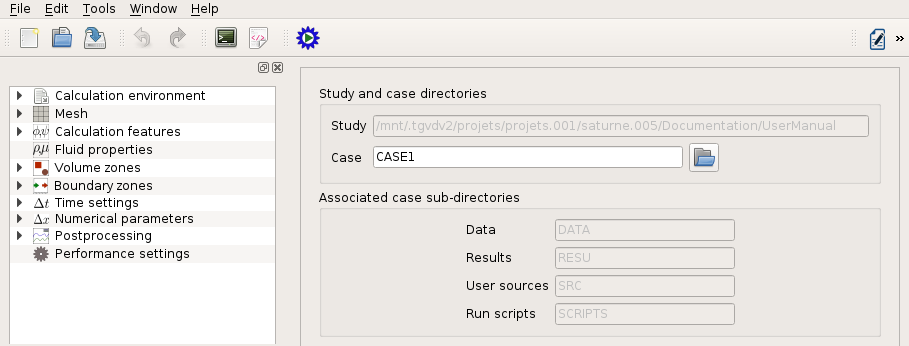
\includegraphics[width=12cm]{gui_case_dir}
\caption{Identity and paths}
\label{fig3_e1}
\end{center}
\end{figure}

\begin{figure}[!ht]
\begin{center}
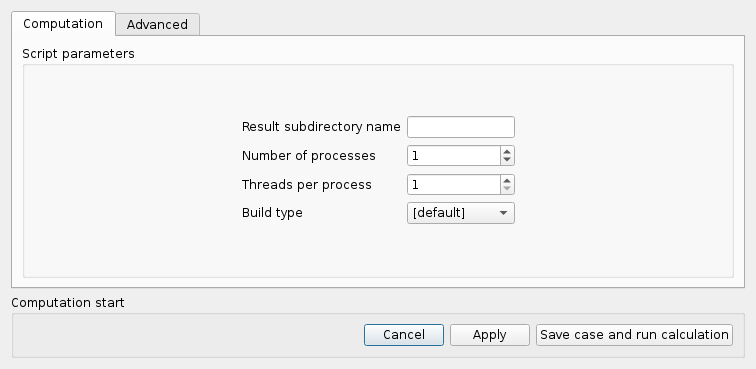
\includegraphics[width=12cm]{gui_prepare_execution}
\caption{Prepare execution}
\label{fig43_e1}
\end{center}
\end{figure}

If no problem arises, the simulation results can be found in the directory \texttt{CASE1/RESU} and be read directly by {\em ParaView} or {\em EnSight} in \texttt{CASE1/RESU/<YYYYMMDD-hhmm>/postprocessing}. Calculation history can be found in the file \texttt{<YYYYMMDD-hhmm>/listing}.

%==================================
\subsection{Troubleshooting}
%==================================
If the calculation does not run properly, the user is advised to check the
following points in\\
\texttt{CASE1/RESU/<YYYYMMDD-hhmm>}:
\begin{list}{$\bullet$}{}
\item  if the calculation stops in the pre-processor, the user should check for error messages in the file \texttt{preprocessor*.log}.
\item if the problem is related to boundary conditions, the user should visualise the file \texttt{error.ensight} with {\em EnSight} or {\em Paraview},
\item if the calculation stops in the \CS core, the user should look for messages at the end of the files \texttt{listing} and \texttt{error*}. In addition, the user can track the following keywords in the listing. They are specific error signals:
  \begin{list}{-}{}
  \item  \texttt{SIGFPE}: a floating point exception occurred. It happens when there is a division by 0, when the calculation did not converge, or when a real number reached a value over $10^{300}$. Depending on the architecture \CS is running
on, this type of execption may be caught or ignored.
  \item  \texttt{SIGSEGV}: a memory error such as a segmentation violation occurred. An array may have exceeded its allocated memory size and a memory location in use was overwritten.
  \end{list}
\end{list}
%==================================
%==================================
\section{Practical information about \CS}
%==================================
%==================================

%==================================
\subsection{System Environment for \CS}
%==================================

%==================================
\subsubsection{Preliminary settings}
%==================================
\label{prg_environementCS}

In order to use \CS, every user must add the following line (in their
\texttt{.profile}, \texttt{.bashrc}, or equivalent,
depending on the environment):

\hspace*{1cm}\texttt{export PATH=\$\{prefix\}/bin:\$PATH}\\

or define the following alias (in their \texttt{.bashrc}, or
 equivalent, or \texttt{.alias} file, depending on the environment):

\hspace*{1cm}\texttt{alias cs='\$\{prefix\}/bin/cs'}\\

where \texttt{prefix} is the base directory where
\CS and its components have been installed\footnote{At EDF R\&D, \texttt{/home/saturne/Code\_Saturne/\verscs} is used}.

%==================================
\subsubsection{Standard directory hierarchy}
%==================================
\label{prg_architecture}%
The standard architecture for the simulation studies is:

\noindent
An optional study directory containing:
\begin{list}{$\bullet$}{}
\item A directory \texttt{MESH} containing the mesh(es)
      necessary for the study
\item A directory \texttt{POST} for the potential post-processing routines (not
used directly by the code)
\item One or several calculation directories
\end{list}

\noindent
Every calculation directory contains:
\begin{list}{$\bullet$}{}
\item A directory \texttt{SRC} for the potential user subroutines
      necessary for the calculation
\item A directory \texttt{DATA} for the calculation data (data
      file from the interface, input profiles, thermo-chemical data, ...)
\item A directory \texttt{SCRIPTS} for the launch script
\item A directory \texttt{RESU} for the results\\
To improve the calculation traceability, the files and directories
sent to \texttt{RESU} after a calculation are  placed in a subdirectory
named after that run's ``id'', which is by default based on the run date
and time, using the format: \texttt{YYYYMMDD-hhmm}.
It is also possible to force a specific run id, using the \texttt{--id}
option to \texttt{code\_saturne run}.
\end{list}

\noindent
In the standard cases, \texttt{RESU/<run\_id>} contains a
\texttt{postprocessing} directory with the post-processing
(visualization) files, a \texttt{restart} directory for the calculation
restart files, a \texttt{monitoring} directory for the files of chronological
record of the results at specific locations (probes),\\
\texttt{preprocessor.log} and \texttt{listing} files reporting the
Preprocessor and the Kernel execution. For an tracing of
the modifications in prior calculations, the user-subroutines used in
a calculation are stored in a \texttt{src\_saturne} subdirectory. The {\em Xml}
Interface data file, thermo-chemical data files and launch script are also
copied into the results directory. \texttt{compil.log} and
\texttt{summary} are respectively reports of the compilation stage and
general information on the calculation (type of machine, user,
version of the code, ...).

\begin{table}[h!t]
\begin{tabular}{lll}
\multicolumn{3}{l}{Below are typical contents of a case directory CASE1 in a study STUDY} \\
\multicolumn{2}{l}{\texttt{STUDY/CASE1/DATA:}}&{\bf \CS data}\\
&        \texttt{SaturneGUI}        &Graphical User Interface launch script\\
&        \texttt{study.xml}         &Graphical User Interface parameter file\\
&        \texttt{REFERENCE}         &Example of user scripts and meteorological\\
&                                   &  or thermochemical date files (used with the\\
&                                   & specific physics modules)\\
\multicolumn{2}{l}{\texttt{STUDY/CASE1/SRC:}}&{\bf \CS user subroutines }\\
&        \texttt{REFERENCE}         &  Examples of a user subroutines\\
&        \texttt{usclim.f90}        &  user subroutines used for the present calculation\\
&        \texttt{usini1.f90} &\\
\multicolumn{2}{l}{\texttt{STUDY/CASE1/RESU/20110509-1920:}}&{\bf results} for the
                                                             calculation 20110509-1920\\
&        \texttt{postprocessing}    &directory containing the \CS post-processing output\\
&                                   &in the {\em EnSight} format (both volume and boundary);\\
&        \texttt{src\_saturne}      &copy of the \CS user subroutines used for the calculation\\
&        \texttt{monitoring}        &directory containing the chronological records for \CS\\
&        \texttt{checkpoint}        &directory containing the \CS restart files \\
&        \texttt{compile.log}       &compilation log\\
&     \texttt{study.xml}            &Graphical User Interface parameter file used for the\\
&                                   &calculation\\
&        \texttt{runcase}           &copy of the launch script used for the calculation\\
&        \texttt{preprocessor.log}  &execution report for the \CS Preprocessor\\
&        \texttt{listing}           &execution report for the Kernel module of \CS\\
&        \texttt{summary}           &general information (machine, user, version, ...)\\
\multicolumn{2}{l}{\texttt{STUDY/CASE1/SCRIPTS:}}&{\bf launch script}\\
&        \texttt{runcase}           &launch script (which may contain batch
                                     system keywords)\\
\end{tabular}
\end{table}

Note that the code may be run directly in the final \texttt{RESU/<run\_id>}
directory, or in a scratch directory (which may be recommended if the
compute environment includes different filesystems, some better suited
to data storage, others to intensive I/O). When running, the code
may use additional files or directories inside its execution directory, set
by the execution script, which include a \texttt{mesh\_input} file or directory,
as well as a \texttt{restart} directory (which is a link or copy of a previous
run's \texttt{checkpoint} directory), as well as a \texttt{run\_solver.sh}
script.

For coupled calculations, whether with \CS or \syrthes, each coupled
calculation domain is defined by its own directory (bearing the same name
as the domain), but results are placed in a \texttt{RESU\_COUPLING}
directory, with a subdirectory for each run, itself containing one
subdirectory per coupled domain. Coupled cases are not run through
the standard {\texttt{STUDY/CASE1/SCRIPTS/runcase} script or through
the {\texttt{code\_saturne run} command, but through a
{\texttt{STUDY/runcase\_coupling} script.

So in the coupled case, calculation results would not be placed in
\texttt{STUDY/CASE1/RESU/20110509-1920}, but in
\texttt{STUDY/RESU\_COUPLING/20110509-1920/CASE1}, with the \texttt{summary}
file being directly placed in \texttt{STUDY/RESU\_COUPLING/20110509-1920}
(as it references all coupled domains).

\begin{table}[h!t]
\begin{tabular}{lll}
\multicolumn{3}{l}{Below are typical additional contents with a coupled \syrthes
  case SOLID1 in a study STUDY} \\
\multicolumn{2}{l}{\texttt{STUDY/runcase\_coupling}}&{coupled launch script}\\
\multicolumn{2}{l}{\texttt{STUDY/SOLID1/DATA:}}&{\bf \syrthes data}\\
&        \texttt{syrthes.data}                &\syrthes data file \\
&        \texttt{syrthes.env}                 &\syrthes configuration file\\
\multicolumn{2}{l}{\texttt{STUDY/RESU\_COUPLING/20110509-1920/SOLID1:}}&{\bf results
 (file names defined in \texttt{syrthes.env})}\\
&        \texttt{src}                &\syrthes user subroutines
                                     used in the calculation\\
&        \texttt{compile.log.08211921}  &\syrthes compilation report\\
&        \texttt{listsyr}            &execution log\\
&        \texttt{geoms}              &\syrthes \ solid geometry file\\
&        \texttt{histos1}            &\syrthes chronological records at
                                                  specified probes\\
&        \texttt{resus1}             &\syrthes calculation restart file (1 time step)\\
&        \texttt{resusc1}            &\syrthes chronological solid
                                      post-processing file\\
&                                    &(may be transformed into the {\em EnSight}
                                      format\\
&                                    &with the {\em syrthes2ensight} utility)\\
\end{tabular}
\end{table}

%==================================
\subsubsection{\CS Kernel library files}
%==================================
\label{prg_library}%
Information about the content of the \CS base directories is given below. It
is not of vital interest for the user, but given only as general
information. Indeed, the case preparer command \texttt{code\_saturne~create}
automatically extracts the necessary files and prepares the launch script
without the user having to go directly into the \CS base directories
(see \S\ref{prg_cscreate}).
The \texttt{code\_saturne~info} command gives direct
access to the most needed information (especially the user and programmer's
guides and the tutorial) without the user having to look for them in the \CS
directories.

The subdirectories \texttt{\{prefix\}/lib} and \texttt{\{prefix\}/bin }
contain the libraries and compiled executables respectively.

The data files (for instance thermochemical data) are located in the
directory \texttt{data}.

The user subroutines are available in the directory \texttt{users},
under subdirectories corresponding to each module:
\texttt{base} (general routines),
\texttt{cfbl} (compressible flows),
\texttt{cogz} (gas combustion),
\texttt{cplv} (pulverised coal combustion),
\texttt{ctwr} (cooling towers modelling),
\texttt{elec} (electric module),
\texttt{fuel} (heavy fuel oil combustion module),
\texttt{lagr} (Lagrangian module,
\texttt{pprt} (general specific physics routines) and
\texttt{rayt} (radiative heat transfer).
The case preparer command \texttt{code\_saturne~create} copies all these files
in the user directory \texttt{SRC/REFERENCE} during the case preparation.

The directory \texttt{bin} contains an example of the launch script, the
compilation parameter files and various utility programs.

%==================================
\subsection{Setting up and running a calculation}
%==================================

%==================================
\subsubsection{Step by step calculation}
%==================================

This paragraph summarises the different steps which are necessary to
prepare and run a standard case:

\begin{list}{$\bullet$}{}

\item Check the version of \CS set for use in the environment variables
(\texttt{code\_saturne~info --version}). If it does not correspond to
the desired version, update the \texttt{.profile} file to set the environment
variables correctly. Log out of the session and
log in again to take the modifications into account properly (cf.
\S\ref{prg_environementCS}).

\item Prepare the different directories using the \texttt{code\_saturne~create}
command (see \S\ref{prg_cscreate}).

\item It is recommendned to place the mesh(es) in the directory \texttt{MESH},
but they may be selected from other directories. Make sure they are
in a format compliant with \CS (see \S\ref{prg_maillages}). There can be
several meshes in case of mesh joining or coupling with
\syrthes\footnote{\syrthes 3 uses meshes composed of 10-node tetrahedra (vertices
and centers of edges, \syrthes 4 uses meshes composed of 4-node tetrahedra}.

\item Go to the directory \texttt{DATA} and launch the
      Graphical User Interface using the command \texttt{./SaturneGUI}.

\item If not using the GUI, copy the
  \texttt{DATA/REFERENCE/cs\_user\_scripts.py} file to \texttt{DATA} and
  edit it, so that the correct run options and paths may be set. For advanced
  uses, this file may also be used in conjunction with the GUI. Jus as with
  user Fortran subroutines below, settings defined in this file have priority
  over those defined in the GUI.

\item Place the necessary user subroutines in the directory \texttt{SRC} (see
\S\ref{prg_ssprgutilis}). When not using the Interface, some subroutines are
compulsory.

\begin{list}{}{}

\item {\bf For the standard physics:}

    \begin{list}{}{}
        \item {\em compulsory without Graphical User Interface:}
        \begin{list}{-}{}
            \item \texttt{usini1} to specify the calculation parameters

            \item \texttt{usclim} to manage the boundary conditions
        \end{list}

        \item {\em  very useful:}
        \begin{list}{-}{}
            \item \texttt{usphyv} to manage the variable physical
                  properties (fluid density, viscosity ...)

            \item \texttt{usiniv} to manage the non-standard initialisations
        \end{list}
    \end{list}

  \item{\bf For the ``gas combustion'' specific physics:}

(not accessible through the Graphical User Interface in version \verscs)
    \begin{list}{}{}
        \item {\em compulsory:}
        \begin{list}{-}{}
            \item \texttt{usini1} to specify the calculation parameters

            \item \texttt{usppmo} to select a specific physics module and
               combustion model

            \item \texttt{usebuc}, \texttt{usd3pc} or \texttt{uslwcc}
                  (depending on the selected combustion model) to manage the
                  boundary conditions of {\em all variables} ({\em i.e.} not only
              the ones related to the combustion model)
        \end{list}

        \item {\em very useful:}
        \begin{list}{-}{}
            \item  \texttt{usebu1}, \texttt{usd3p1} or \texttt{uslwc1}
                   (depending on the selected combustion model)
               to specify the calculation options
                   for the variables
                   corresponding to combustion model

            \item   \texttt{usebui}, \texttt{usd3pi} or \texttt{uslwci}
              (depending on the selected combustion model)
                   to manage the initialisation of the variables
                   corresponding to the combustion model
        \end{list}
    \end{list}

  \item{\bf For the ``coal combustion'' specific physics:}

    \begin{list}{}{}
        \item {\em compulsory without Graphical User Interface:}
        \begin{list}{-}{}
            \item \texttt{usini1} to specify the calculation parameters

            \item \texttt{usppmo} to select the specific physics module

            \item \texttt{uscpcl} or \texttt{uscplc} (depending on the
                  specific physics module) to manage the
                  boundary conditions of {\em all variables} ({\em i.e.} not only
              the ones related to the specific physics module)
        \end{list}

        \item {\em very useful:}
        \begin{list}{-}{}
            \item  \texttt{uscpi1}
               to specify the calculation options
                   for the variables
                   corresponding to the specific physics module

            \item \texttt{uscpiv} to manage the initialisation of the
                   variables corresponding to the specific physics module
        \end{list}
    \end{list}

     \item{\bf For the ``electric module'' specific physics
      (Joule effect and electric arcs):}

(not accessible through the Graphical User Interface in version \verscs)
    \begin{list}{}{}
       \item {\em compulsory:}
        \begin{list}{-}{}
            \item \texttt{usini1} to specify the calculation parameters

            \item \texttt{usppmo} to select the specific physics module

            \item \texttt{uselcl} to manage the boundary conditions of {\em all
              variables} ({\em i.e.} not only
              the ones related to the electric module)

            \item \texttt{useliv} to initialise the enthalpy in
                  case of Joule effect

            \item \texttt{uselph} to define the physical
                  properties in case of Joule effect
        \end{list}

        \item {\em very useful:}
        \begin{list}{-}{}
            \item  \texttt{useli1} to manage the options related
                   to the variables corresponding to the electric module

            \item   \texttt{useliv} to manage the initialisation of the
                   variables corresponding to the electric module
        \end{list}
    \end{list}

     \item{\bf For the ``heavy fuel oil combustion module'' specific physics:}

(not accessible through the Graphical User Interface in version \verscs)
    \begin{list}{}{}
        \item {\em compulsory:}
        \begin{list}{-}{}
            \item \texttt{usini1} to specify the calculation parameters

            \item \texttt{usppmo} to select the specific physics module

            \item \texttt{usfucl} to manage the
                  boundary conditions of {\em all variables} ({\em i.e.} not only
              the ones related to the specific physics module)
        \end{list}

        \item {\em very useful:}
        \begin{list}{-}{}
            \item  \texttt{usfui1}
               to specify the calculation options
                   for the variables
                   corresponding to the specific physics module

            \item \texttt{usfuiv} to manage the initialisation of the
                   variables corresponding to the specific physics module
        \end{list}
    \end{list}


    \item{\bf For the Lagrangian module (dispersed phase):}

(the continuous phase is managed in the same way as for a case of standard
physics)\\
(the Lagrangian module is not accessible through the Graphical User Interface in
version \verscs)
    \begin{list}{}{}
        \item {\em compulsory:}
        \begin{list}{-}{}
            \item \texttt{uslag1} to manage the calculation conditions

            \item \texttt{uslag2} to manage the boundary conditions for the
             dispersed phase

        \end{list}

        \item {\em very useful:}
        \begin{list}{-}{}
                \item \texttt{uslabo} to manage potential specific treatments at the
             boundaries (rebound conditions, specific statistics, ...)
        \end{list}
    \end{list}

   \item {\bf For the compressible module:}

(not accessible through the Graphical User Interface in version \verscs)
    \begin{list}{}{}
        \item {\em compulsory:}
        \begin{list}{-}{}
            \item \texttt{uscfx1} and \texttt{uscfx2} to manage the
                  calculation parameters

            \item \texttt{uscfcl} to manage the boundary conditions

            \item \texttt{uscfth} to define the thermodynamics.
        \end{list}

        \item {\em very useful:}
        \begin{list}{-}{}
                \item \texttt{uscfxi} to manage non-standard initialisations of the variables
        \end{list}
    \end{list}

\end{list}


The comprehensive list of the user subroutines and their instructions
      for use are given in \S\ref{prg_ssprgutilis}.

\item If necessary, place in the directory \texttt{DATA} the different
      external data (input profiles, thermochemical data files, ...)

\item Prepare the launch script \texttt{runcase}, directly or through the
      Graphical Interface (see \S\ref{prg_runcase}), or prepare the
      \texttt{DATA/cs\_user\_scripts.py} file.

\item Run the calculation and analyse the results

\item Purge the temporary files (in \texttt{RESU/<run\_id>} or
      \texttt{<scratch>/<run\_id>} directory).
\end{list}


%==================================
\subsubsection{Temporary execution directory}
%==================================
\label{prg_temporarydirectory}%
During a calculation, \CS may use a temporary directory for the compilation and
the execution if such a ``scratch'' directory is defined. In that case, the
result files are only copied at the end in the directory
\texttt{RESU}. This is recommended if the compute environment includes different
filesystems, some better suited to data storage, others to intensive I/O.
If this is not the case, there is no point in running in a scratch directory
rather than the results directory, as this incurs additional file copies.

\noindent
{\em WARNING: in case of an error, the temporary directories are not deleted
after a calculation, so that they may be used for debugging. They may then
accumulate and may hinder the correct operation of the machine.\\
\centerline{\bf It is therefore essential to remove them regularly.}}


%==================================
\subsubsection{Execution modes}
%==================================
\label{prg_executionmodes}%
As explained before, \CS is composed of two main modules, the Preprocessor and the
Kernel, and an optional Partitioner. The Preprocessor reads the meshes.
The Partitioner optimizes domain decomposition for parallel runs.
The resulting data is transfered to the Kernel through specific
files, named \texttt{mesh\_input} and \texttt{domain\_number\_*}, where
\texttt{*} is the number of processors used. In a standard calculation, the files
are not copied from the temporary execution directory to the results directory,
as they have no interest for data analysis, and are considered ``internal''
files, whose format or contents is not guaranteed not to change between \CS versions.

Yet, the Preprocessor does not run in parallel and may require a
large amount of memory. Similarly, the Partitioner may be run on a
reduced number of processors to obtain a better partition quality, so it
is sometimes useful to run the Preprocessor and Partitioner
separately, on a machine or in batch queues with extended memory, and to run the
proper parallel calculation on another machine or in another batch
queue. The launch scripts therefore allows specifically choosing
which modules to run, either through the GUI or through \texttt{cs\_user\_scripts.py}:

\sloppy

\hspace*{0.5cm} If a {mesh\_input} file or directory is defined (which may be
either a {mesh\_input} from a previous Preprocessor run or a {mesh\_output}
from a previous solver run), the script will copy or link it to
the execution directory, and the Preprocessor will not be run again.

\hspace*{0.5cm} If \texttt{domain.exec\_partition = False}, the Partitioner
will not be run. A previous partitioning may be used by defining the
\texttt{domain.partition\_input} path.

\hspace*{0.5cm} If \texttt{domain.exec\_kernel = False}, the Kernel will not
be run. This is useful when only the mesh import and optionnaly partitioning
stages are required.

\fussy

It is encouraged to separate the mesh import and calculation runs, as
this speeds up calculations by not re-importing meshes for each run.
For some configurations, such as IBM Blue Gene machines with different
front-end an compute nodes, mesh import may be impossible on the
compute nodes (as the Preprocessor does not run in parallel, and may require
too much memory), so mesh import (and serial partitioning) should be
run separately on the front-end nodes, while later calculation stages
should be run on compute nodes.

Note also that depending on its configuration, the Partitioner may
be run either or both in serial or parallel mode. By default, serial
mode is currently chosen (due to limited feedback on partitioning
quality in parallel mode), but setting \texttt{domain.partition\_n\_procs}
to a value greater than 1 in the user scripts allows running
the Partitioner in parallel.

%==================================
\subsubsection{Interactive modification of the target time step}
%==================================
\label{prg_ficstp}%
During a calculation, it is possible to change the limit time step number
(\texttt{ntmabs}) specified through the Interface or in \texttt{usini1}.
To do so, a file named \texttt{ficstp} must be placed in the temporary
execution directory (see \S\ref{prg_temporarydirectory}).
This file must contain a blank first line and
the second line indicating the value of the new limit number of time steps.\\
If this new limit has already been passed in the calculation, \CS will stop
properly at the end of the current time step (the results and restart files
will be written correctly).\\
This procedure allows the user to stop a calculation in a clean and interactive
way whenever they wish.


%==================================
\subsection{Case preparer}
%==================================
\label{prg_cscreate}%
The case preparer command \texttt{code\_saturne~create} automatically creates a
study directory according to the typical architecture and copies and
pre-fills an example of calculation launch script.

The syntax of \texttt{code\_saturne~create} is as follows:

\noindent
\texttt{code\_saturne~create --study STUDY CASE\_NAME1 CASE\_NAME2...}\\
creates a study directory \texttt{STUDY} with case subdirectories
\texttt{CASE\_NAME1} and \texttt{CASE\_NAME2}...
If no case name is given, a default case directory called \texttt{CASE1} is
created.

\noindent
\texttt{code\_saturne~create --case DEBIT3 --case DEBIT4}\\
executed in the directory \texttt{STUDY} adds the case directories
\texttt{DEBIT3} and \texttt{DEBIT4}.

An option \texttt{--nogui} is available for the use of \CS
without Graphic Interface. This option must
be either the first or the last argument and appear only once.

In the directory \texttt{DATA}, the \texttt{code\_saturne~create} command
places a subdirectory \texttt{THCH} containing examples of thermochemical data
files used for pulverised coal combustion,
gas combustion or electric arc. The file to be used for the calculation must be
copied directly in the \texttt{DATA} directory and its name must be referenced
in the launch script in the variable THERMOCHEMISTRY\_DATA. All other files in
the \texttt{DATA} or in the \texttt{THCH} will be ignored.\\
The \texttt{code\_saturne~create} command also places in the directory
\texttt{DATA} the launch script for the Graphical User Interface:
\texttt{SaturneGUI}.


In the directory \texttt{SRC}, the \texttt{code\_saturne~create} command creates a
subdirectory \texttt{REFERENCE} containing all the user subroutines,
classified by module type:  \texttt{base},
\texttt{cfbl}, \texttt{cogz}, \texttt{cplv}, \texttt{elec}, \texttt{fuel},
\texttt{lagr}, \texttt{pprt} and \texttt{rayt}.
Only the user subroutines placed directly under
the directory \texttt{SRC} will be considered. The others will be ignored.

In the directory \texttt{SCRIPTS}, the \texttt{code\_saturne~create} command copies and
pre-fills an example of the launch script: \texttt{runcase}.
The study, case and user name are filled
automatically in the launch script, as are the paths leading to the
different directories. Other parameters must be specified in the script
(see \S\ref{prg_runcase}),
especially the mesh file(s) to use, but everything can be specified
through the Graphical Interface.

\smallskip \noindent

%==================================
\subsection{Supported mesh and post-processing output formats
\label{sec:formats}}
%==================================

\CS supports multiple mesh formats, all of these having been requested
at some time by users or projects based on their meshing or post-processing
tools. All of these formats have advantages and disadvantages (in terms
of simplicity, functionality, longevity, and popularity) when compared to
each other. The following formats are currently supported by \CS:

\begin{list}{-}{}

\item \hyperref[fmtdesc:des]{\simail (NOPO)}
\item \hyperref[fmtdesc:unv]{\ideas universal}
\item \hyperref[fmtdesc:med]{\med}
\item \hyperref[fmtdesc:cgns]{CGNS}
\item \hyperref[fmtdesc:ensight6]{\ensight 6}
\item \hyperref[fmtdesc:ensightg]{\ensightg}
\item \hyperref[fmtdesc:neu]{\gambit neutral}
\item \hyperref[fmtdesc:gmsh]{\gmsh}
\item \hyperref[fmtdesc:ngeom]{pro-STAR/STAR4}
\item \hyperref[fmtdesc:ccm]{STAR-CCM+}
\end{list}

These formats are described in greater detail in the following sections.
Unless a specific option is used, the \pcs determines the mesh format directly
from the file suffix: %
{\em``\texttt{.case}''} for \ensight (6 or Gold),
{\em``\texttt{.ccm}''} for STAR-CCM+,
{\em``\texttt{.cgns}''} for CGNS,
{\em``\texttt{.des}''} for \simail,
{\em``\texttt{.med}''} for \med,
{\em``\texttt{.msh}''} for \gmsh,
{\em``\texttt{.neu}''} for \gambit neutral,
{\em``\texttt{.ngeom}''} for pro-STAR/STAR4,
{\em``\texttt{.unv}''} for I-deas universal.

Note that the preprocessor can read gzipped mesh files directly (for Formats
other than MED or CGNS, which use specific external libraries) on most machines.

%==================================
\subsubsection{Formats supported for input\label{sec:formats_in}}
%==================================

\subsubsubsection{NOPO/\simail (INRIA/SIMULOG)%
\label{fmtdesc:des}}

This format output by \simail is still heavily used at EDF. We do not
currently handle cylindrical or spherical coordinates, but it seems that
\simail always outputs meshes in Cartesian coordinates, even if points
have been defined in another system. Most ``classical'' element types
are usable, except for pyramids.

Note that depending on the architecture on which a file was
produced by \simail,\footnote{``little endian'' on Intel or AMD processors, or
``big endian'' on most others, and starting with \simail 7, 32-bit or 64-bit
 integer and floating-point numbers depending on architecture},
it may not be directly readable by \simail on a different machine, while
this is not a problem for the \pcs, which automatically detects the
byte ordering and the 32/64 bit variant and adjusts accordingly.

\smallskip \noindent
\begin{tabular}[top]{|p{4.5cm}%
                     |>{\PreserveBackslash\raggedright\hspace{0pt}}p{10.5cm}|}
\hline
Default extension: & {\tt .des}\\
\hline
File type:         & semi-portable ``Fortran'' binary (IEEE integer and
                     floating-point numbers on 4 or 8 bytes, depending on
                     32 or 64 bit \simail version, bytes also ordered based
                     on the architecture)\\
\hline
Surface elements:  & triangles, quadrangles
                     (+ volume element face references)\\
\hline
Volume elements:   & tetrahedra, prisms, hexahedra\\
\hline
Zone selection:    & element face references and volume sub-domains\\
                   & (interpreted as numbered groups)\\
\hline
Compatibility:     & all files of this type as long as the coordinate
                     system used is Cartesian and not cylindrical or
                     spherical\\
\hline
Documentation:     & Simail user documentation and release notes or
                     MODULEF documentation:
                     \url{http://www-rocq.inria.fr/modulef} \par
                     Especially: \par
                     \url{http://www-rocq.inria.fr/modulef/Doc/FR/Guide2-14/node49.html} \\
\hline
\end{tabular}

\subsubsubsection{\ideas universal file%
\label{fmtdesc:unv}}

This format was very popular in the 1990's and early 2000's, and though
the I-deas tool has not focused on the CFD (or even meshing) market since
many years, it is handled (at least in part) by many tools, and may
be considered as a major ``legacy'' format. It may contain many different
datasets, relative to CAD, meshing, materials, calculation results,
or part representation. Most of these datasets are ignored by \CS,
and only those relative to vertex, element, group, and coordinate system
definitions are handled.

This format's definition evolves with \ideas versions, albeit in a limited
manner: some datasets are declared obsolete, and are replaced by others,
but the definition of a given dataset type is never modified. Element and
Vertex definitions have not changed for many years, but group definitions
have gone through several dataset variants through the same period,
usually adding minor additional group types not relevant to meshing.
If one were to read a file generated with a more recent version of \ideas
for which this definitions would have changed with no update in the \pcs,
as the new dataset would be unknown, it would simply be ignored.

Note that this is a text format. Most element types are handled, except
for pyramids.

\smallskip \noindent
\begin{tabular}[top]{|p{4.5cm}%
                     |>{\PreserveBackslash\raggedright\hspace{0pt}}p{10.5cm}|}
\hline
Default extension: & {\tt .unv}\\
\hline
File type:         & text\\
\hline
Surface elements:  & triangles, quadrangles\\
\hline
Volume elements:   & tetrahedra, prisms, hexahedra\\
\hline
Zone selection:    & colors (always) and named groups\\
\hline
Compatibility:     & \ideas (\emph{Master Series} 5 to 9, \emph{NX Series} 10 to 12)
                     at least\\
\hline
Documentation:     & Online I-deas NX Series documentation\\
\hline
\end{tabular}

\subsubsubsection{\gambit neutral%
\label{fmtdesc:neu}}

This format may be produced by Ansys \fluent's GAMBIT meshing tool.
As this tool does not export meshes to other formats directly handled
by the \pcs (though \fluent itself may export files to the CGNS or
\ideas universal formats), it was deemed useful to enable the \pcs
to directly read files in \gambit neutral format.

Note that this is a text format. ``Classical'' element types are usable.

\smallskip \noindent
\begin{tabular}[top]{|p{4.5cm}%
                     |>{\PreserveBackslash\raggedright\hspace{0pt}}p{10.5cm}|}
\hline
Default extension: & {\tt .neu}\\
\hline
File type:         & text\\
\hline
Surface elements:  & triangles, quadrangles\\
\hline
Volume elements:   & tetrahedra, pyramids, prisms, hexahedra\\
\hline
Zone selection:    & boundary conditions for faces, element groups for cells\\
                   & (interpreted as named groups)\\
\hline
Documentation:     & GAMBIT on-line documentation\\
\hline
\end{tabular}

\subsubsubsection{pro-STAR%
\label{fmtdesc:ngeom}}

This polyhedral format from CD-Adapco seems to be usable both with the
\starcd and \starccmp tools, and the \textbf{pro-STAR} tool should be able to
generate it. The test meshes we have were generated by the
\textbf{Comet-Design} tool, which has since been replaced by other
CD-Adapco tools, especially \starcd V4 and \starccmp. The available
test cases are thus not extensive in terms of functionality (especially
when considering definition of descriptions), so support for this format
is lightly tested.

Currently, geometric entity numbers are converted to group numbers.
This tends to lead to a large number of groups.

\smallskip \noindent
\begin{tabular}[top]{|p{4.5cm}%
                     |>{\PreserveBackslash\raggedright\hspace{0pt}}p{10.5cm}|}
\hline
Default extension: & {\tt .ngeom}\\
\hline
File type:         & binary file using portable XDR encoding.\\
\hline
Surface elements:  & polygons\\
\hline
Volume elements:   & polyhedra\\
\hline
Zone selection:    & face and cell sets\\
                   & (interpreted as numbered groups)\\
\hline
Compatibility:     & all files of this type ? (tested on purely polyhedral meshes)\\
\hline
Documentation:     & documentation accompanying and source code provided by CD-adapco in
                     the context of a collaboration with UMIST (now
                     University of Manchester) and EDF R\&D/MFEE\\
\hline
\end{tabular}

\subsubsubsection{\starccmp%
\label{fmtdesc:ccm}}

This polyhedral format is the current CD-Adapco format, and is based on
CD-Adapco's libccmio, which is based on ADF (the low-level file format
used by CGNS prior to the shift to HDF-5). libccmio comes with a version
of ADF modified for performance, but also works with a standard version
from CGNS.

Currently, geometric entity numbers are converted to numbered groups,
with the corresponding names printed to the \pcs log. Depending on whether
the names were generated automatically or set by the user, it would be
preferable to use the original group names rather than base their
names on their numbers.

The CCMIO library is distributed freely by CD-Adapco upon demand.

\smallskip \noindent
\begin{tabular}[top]{|p{4.5cm}%
                     |>{\PreserveBackslash\raggedright\hspace{0pt}}p{10.5cm}|}
\hline
Default extension: & {\tt .ccm}\\
\hline
File type:         & binary file using modified ADF library.\\
\hline
Surface elements:  & polygons\\
\hline
Volume elements:   & polyhedra\\
\hline
Zone selection:    & named face and cell sets\\
                   & (interpreted as numbered groups, with names appearing in log)\\
\hline
Compatibility:     & all files of this type ? (tested on purely polyhedral meshes)\\
\hline
Documentation:     & documentation and source code provided by CD-adapco\\
\hline
\end{tabular}

\subsubsubsection{\ensight 6%
\label{fmtdesc:ensight6}}

This format is used for output by the \harpoon meshing tool, developed
by Sharc Ltd (also the distributor of \ensight for the United Kingdom).
This format may represent all ``classical'' element types.

Designed for post processing, it does not explicitely handle the definition
of surface patches or volume zones, but allows the use of many \emph{parts}
(i.e. groups of elements) which use a common vertex list.
A possible convention (used at least by \harpoon) is to add surface
elements to the volume mesh, using one \emph{part} per group. The volume
mesh may also be separated into several \emph{parts} so as to identify
different zones. As \emph{part} names may contain up to 80 characters,
we do not transform them into groups (whose names could be unwieldy),
so we simply convert their numbers to group names.

Also note that files produced by \harpoon may contain badly oriented
prisms, so the \pcs orientation correction option
(\texttt{--reorient})may need to be used. Meshes built by this tool also
contain hanging nodes, with non-conforming elements sharing some vertices.
Mesh joining must thus also be used, and is not activated automatically,
as the user may prefer to specify which surfaces should be joined,
and which ones should not (i.e. to conserve thin walls).

\smallskip \noindent
\begin{tabular}[top]{|p{4.5cm}%
                     |>{\PreserveBackslash\raggedright\hspace{0pt}}p{10.5cm}|}
\hline
Default extension: & {\tt .case}\\
\hline
File type:         & text file (extension \emph{.case}), and text,
                     binary, or Fortran binary file with 
                     (\emph{.geo} extension), describing the  integers
                     describing integers and floats in the IEEE format,
                     using 32 bits\\
\hline
Surface elements:  & triangles, quadrangles\\
\hline
Volume elements:   & tetrahedra, pyramids, prisms, hexahedra\\
\hline
Zone selection:    & part numbers interpreted as numbered groups\\
\hline
Compatibility:     & All files of this type\\
\hline
Documentation:     & online documentation, also available at:
                     \href{http://www.ensight.com/downloads/cat\_view-5.html}
                          {http://www.ensight.com/downloads/cat\_view-5.html}\\
\hline
\end{tabular}

\subsubsubsection{\gmsh%
\label{fmtdesc:gmsh}}

This format is used by the free \href{http://www.geuz.org/gmsh}{\gmsh}
tool. This tool has both meshing and post-processing functionality,
but \CS only imports meshes.

Note that some meshes produced by\gmsh man contain some badly oriented
elements, so the \pcs's \texttt{-reorient} option may be necessary.

The \pcs handles versions 1 and 2 of this array. In version 1,
two labels are associated with each element: the first defines the
element's physical entity  number, the second defines it' elementary
entity number. Using version 2, it is possible to associate an
arbitrary number of labels with each element, but files produced
by \gmsh use 2 labels, with the same meanings as with version 1.

We chose to convert physical entity numbers to groups. It is possible
to build a mesh using \gmsh without defining any  physical entities
(in which case all elements will belong to the same group, but the \gmsh
documentation clearly says that geometric entities are to be used
so as to group elementary entities having similar ``physical'' meanings.

So as to obtain distinct groups with a mesh generated by \gmsh, it
is thus necessary for the user to define physical entities.
This requires an extra step, but allows for fine-grained control
over the groups associated with the mesh, while using only elementary
entities could lead to a high number of groups.

\smallskip \noindent
\begin{tabular}[top]{|p{4.5cm}%
                     |>{\PreserveBackslash\raggedright\hspace{0pt}}p{10.5cm}|}
\hline
Default extension: & {\tt .msh}\\
\hline
File type:         & text or binary file\\
\hline
Surface elements:  & triangles, quadrangles\\
\hline
Volume elements:   & tetrahedra, pyramids, prisms, hexahedra\\
\hline
Zone selection:    & physical entity numbers interpreted as numbered groups\\
\hline
Compatibility:     & all files of this type\\
\hline
Documentation:     & included documentation, also available at:
                     \href{http://www.geuz.org/gmsh}
                          {http://www.geuz.org/gmsh}\\
\hline
\end{tabular}

%==================================
\subsubsection{Formats supported for input or output\label{cha:formats_inout}}
%==================================

\subsubsubsection{\ensightg%
\label{fmtdesc:ensightg}}

This format may represent all ``classical'' element types, as well as
arbitrary polygons and convex polyhedra.

This format evolves slightly from one \ensight version to another, keeping
backwards compatibility. For example, polygons could not be used in the
same \emph{part} as other element types prior to version 7.4, which removed
this restriction and added support for polyhedra. Version 7.6 added support
for material type definitions.

This format offers many possibilities not used by \CS, such as defining
values on part of a mesh only (using ``undefined'' marker values or
partial values), assigning materials to elements, defining rigid
motion, or defining per-processor mesh parts with ghost cells for
parallel runs. Note that some libraries allowing direct \ensightg support
do not necessarily support the whole format specification.
Especially, VTK does not support material types, and has only recently
added support for polyhedral elements in \ensightg files (interpreted
as convex point sets in \paraview versions 2.4 to 2.8, and as true
polyhedra starting with \paraview versions 2.10).
Also, both \ensightg (8.2 and above) and VTK allow for automatic distribution,
reducing the usefulness of pre-distributed meshes with per-processor files.

This format may be used as an input format, similar to \ensight 6.
Compared to the latter, each \emph{part} has its own coordinates and vertex
connectivity, so as a convention, we consider that surface or
volume zones may only be considered to be part of the same mesh
if the file defines vertex IDs (which we consider to be
unique vertex labels). In this case, \emph{part} numbers
are interpreted as group names. Without vertex IDs, only one part is read,
and no groups are assigned.

\smallskip \noindent
\begin{tabular}[top]{|p{4.5cm}%
                     |>{\PreserveBackslash\raggedright\hspace{0pt}}p{10.5cm}|}
\hline
Default extension: & {directory {\tt{{\it \{case\_name\}}.ensight}},
                     containing a file with the \tt .case} extension\\
\hline
File type:         & multiple binary or text files\\
\hline
Surface elements:  & triangles, quadrangles, polygons\\
\hline
Volume elements:   & tetrahedra, pyramids, prisms, hexahedra, convex polyhedra\\
\hline
Zone selection:    & possibility of defining element materials (not used), or
                     interpret part number as group name if vertex IDs are
                     given\\
\hline
Compatibility:     & files readable by \ensight 7.4 to 9.0, as well as tools
                     based on the \href{http://www.vtk.org}{\vtk} library,
                     especially \paraview\ (\url{http://www.paraview.org})\\
\hline
Documentation:     & online documentation, also available at:
                     \url{http://www.ensight.com/downloads/cat\_view-5.html}\\
\hline
\end{tabular}

\subsubsubsection{\med}\hyperdef{sec}{med}{}
\label{fmtdesc:med}

Initially defined by EDF R\&D, this format (\emph{Mod\`ele d'\'echanges de Donn\'ees},
or \emph{Model for Exchange of Data}) has been defined and maintained through
a \med working group comprising members of EDF R\&D and CEA (the \CS team
being represented). This is the reference format for the
\href{http://www.opencascade.org/SALOME/Salome.html}{\emph SALOME} environment.
This format is quite complete, allowing the definition of all ``classical''
element types, in nodal or descending connectivity.
It may handle polygonal faces and polyhedral cells,
as well as the definition of structured meshes.

This format, which requires a library also depending on the free HDF5 library,
allows both for reading and writing meshes with their attributes (``families'' of
color/attribute and group combinations), as well as handling calculation data,
with the possibility (unused by \CS) of defining variables only on a subset
(``profile'') of a mesh.

The \med library is available under a \href{http://www.gnu.org}{LGPL} licence,
and is even packaged in some Linux distributions
(at least Debian and Ubuntu). \CS requires at least \med 3.0.2, which in turn
requires HDF5 1.8. This format is upwards-compatible with \med 2.3,
so files in that version of the format may be read, though not output.

\smallskip \noindent
\begin{tabular}[top]{|p{4.5cm}%
                     |>{\PreserveBackslash\raggedright\hspace{0pt}}p{10.5cm}|}
\hline
Default extension:    & {\tt .med}\\
\hline
File type:            & portable binary, based on the HDF5 library
                       (\url{http://www.hdfgroup.org/HDF5/index.html})\\
\hline
Surface elements:     & triangles, quadrangles, simple polygons\\
\hline
Volume elements:      & tetrahedra, pyramids, prisms, hexahedra, simple polyhedra\\
\hline
Zone selection:       & element families ({\it i.e.} colors and groups)\\
\hline
Input compatibility:  & \med 2.3 or \med 3.0
                     (only unstructured nodal connectivity is supported)\\
\hline
Output compatibility: & \med 3.0 and above \\
\hline
Documentation:        & online documentation. Download link at \url{http://files.salome-platform.org/Salome/other/med-3.0.4.tar.gz}\\
\hline
\end{tabular}

\subsubsubsection{CGNS 2.5 or CGNS 3.1}\hyperdef{sec}{cgns}{}
\label{fmtdesc:cgns}

Promoted especially by NASA, Boeing, and ICEM~CFD (as well as ONERA in France),
this format(\emph{CFD General Notation System}) is quite well established in
the world of CFD. The concept is similar to that of \med, with a bigger
emphasis on normalization of variable names or calculation information, and
even richer possibilities. The opposite of \med, the first version of this format
was limited to multibloc structured meshes, unstructured meshes having been
added in CGNS 2.

Slightly older than \med, this library was free from the start, with a good
English documentation, and is thus much better known. It is more focused
on CFD, where \med is more generic. A certain number of tools accompany
the CGNS distribution, including a mesh visualizer (which does not handle
polygonale faces although the format defines them), and an interpolation
tool.

We should be able to read almost any mesh written in this format, though
meshes with overset interfaces may not be usable for a calculation.
Other (abutting) interfaces are not handled automatically (as there are
at least 3 or 4 ways of defining them, and some mesh tools do not export
them\footnote{For example, \icemcfd can join non-conforming meshes, but it
exports joining surfaces as simple boundary faces with user-defined boundary
conditions.}), so the user is simply informed of their existence in the
\pcs's log file, with a suggestion to use an appropriate conformal joining
option. Structured zones are converted to unstructured zones immediately after
being read.

Boundary condition information is interpreted as groups with the same
name. The format does not yet provide for selection of volume elements,
as only boundary conditions defined in the model (and can be assigned to
faces in the case of unstructured meshes, or vertices in any case).
Note that boundary conditions defined at vertices are not ignored by
the \pcs, but are assigned to the faces of which all vertices bear
the same condition.\footnote{If one of a face's vertices does not bear
a boundary condition, that condition is not transferred to the face.}

The \pcs also has the capability of building additional volume or surface groups,
based on the mesh sections to which cells or faces belong. This may be
activated using a sub-option of the mesh selection, and allows obtaining
zone selection information from meshes that do not have explicit
boundary condition information but that are subdivided in appropriate zones or
sections (which depends on the tool used to build the mesh).

When outputting to CGNS, an unstructured connectivity is used for the calculation
domain, with no face joining information or face boundary condition
information.\footnote{Older versions of the documentation specified that
a field must be defined on all elements of a zone, so that adding faces
on which to base boundary conditions to a volume mesh would have required
also defining volume fields on these faces. More recent versions of the
documentation make it clear that a field must be defined on all elements
of maximum dimension in a zone, not on all elements.} 

Though many tools support CGNS, that support is often quite dissapointing,
at least for unstructured meshes. Thus, some editors seem to use
different means to mark zones to associate with boundary conditions than
the ones recommended in the CGNS documentation, and some behaviors
are worse: for example, under \ensightg 8, whenever a mesh
contains multiple element types, variables are assigned to the wrong cells.
Regarding support of polygons (\emph{ngons} in the CGNS standard), even the
verification tools published alongside the CGNS library are unable
to handle them, and report errors in valid files containing such elements.
VisIt 1.11.1 reports an error when a mesh contains such faces, while
\ensightg 8 ignores them. CGNS 3 allows for polyhedra, but as this is a
recent developpement, it is not supported yet by \CS.

\smallskip \noindent
\begin{tabular}[top]{|p{4.5cm}%
                     |>{\PreserveBackslash\raggedright\hspace{0pt}}p{10.5cm}|}
\hline
Default extension: & {\tt .cgns}\\
\hline
File type:         & portable binary (uses the ADF library specific to CGNS, or HDF5)\\
\hline
Surface elements:  & triangles, quadrangles, simple polygons\\
\hline
Volume elements:   & tetrahedra, pyramids, prisms, hexahedra\\
\hline
Zone selection:    & Surface zone selection using boundary conditions, no volume zone
                     selection, but the \pcs allows creation of groups associated to
                     zones or sections in the mesh using mesh selection sub-options\\
\hline
Compatibility:     & CGNS 2.5 or CGNS 3.1\\
\hline
Documentation:     & See CGNS site: \url{http://www.cgns.org}\\
\hline
\end{tabular}

%==================================
\subsubsection{Meshing tools and associated formats}
%==================================

Most often, the choice of a mesh format is linked to the choice of
a meshing tool. Still, some tools allow exporting a mesh under several
formats handled by \CS. This is the case of \fluent and \icemcfd,
which can export meshes to both the \ideas universal and CGNS formats
(\fluent's \gambit is also able to export to \ideas universal format).

Traditionally, users exported files to the \ideas universal format,
but it does not handle pyramid elements, which are often used by these
tools to transition from hexahedral to tetrahedral cells in the case
of hybrid meshes. The user is encouraged to export to CGNS, which
does not have this limitation.

Tools related to the \salome platform should preferably use
\salome{}'s native \med format (export to \ideas universal is
also possible, but has some limitations).

The use of files of the ``Common Solver'' type\footnote{File type specifically
developed for the early prototype versions of \CS (\texttt{tlc}) extension}
is still in part possible but is deprecated. Such files are read directly
from the Kernel, and this format is not handled by the launch
scripts anymore. Many potentialities of \CS are not
usable with this file format (mesh joining with hanging nodes, periodicity,
parallel computing, ...).

%==================================
\subsubsection{Meshing remarks}
%==================================
\label{prg_maillages}%

{\em WARNING: }
Some turbulence models ($k-\varepsilon$, $R_{ij}-\varepsilon$ SSG, ...) used in
\CS are ``High-Reynolds'' models. Therefore the size of the cells
neighboring the wall needs to be greater than the thickness of the viscous
sublayer (at the wall, $y^+>2.5$ is required, and $30<y^+<100$ is
preferable). If the mesh does not match this constraint, the results may
be false (particularly if thermal phenomena are involved). For more details
on these constraints, see the keyword \texttt{ITURB}.

%==================================
\subsection{Preprocessor command line options}
%==================================
\label{prg_optappelecs}%
The main options are:
\begin{list}{$\bullet$}{}
\item \texttt{--help}: gives a summary of the different command line options

\item \texttt{<mesh>}: the last argumen is used to specify the name of the mesh file.
The launch script automatically calls the Preprocessor for every
mesh in the \texttt{MESHES[]} list specified by th user.

\item \texttt{--reorient}: try to re-orient badly-oriented cells
if it is necessary to compensate for mesh-generation software
whose output does not conform to the format specifications.

\end{list}

%==================================
\subsection{Kernel command line options}
%==================================
\label{prg_optappelnoy}%
In the standard cases, the compilation of \CS and its execution are entirely
controlled by the launch script. The potential command line options are passed
through user modifiable variables at the beginning of the script. This way, the
user only has to fill these variables and doesn't need
to search deep in the script for the Kernel command line. For more advanced
usage, the main options are described below:

\begin{list}{$\bullet$}{}
\item \texttt{--solcom}: this option indicates that the Kernel will read the
mesh directly, not using the Preprocessor output files. This is only possible
with ``Common Solver'' type of mesh files (see \S\ref{prg_maillages} for
restrictions).\\
This option is obsolete, and is not handled by the launch script anymore.

\item \texttt{--app-name}: specifies the application name. This is
useful only in the case of code coupling, where the application name
is used to distinguish between different code instances launched together.

\item \texttt{--mpi}: specifies that the calculation is running
with MPI communications. The number of processors used will be determined
automatically by the Kernel. With most MPI implementations, the
code will detect the presence of an MPI environment automatically, and
this option is redundant. It is only kept for the rare case in which the
MPI environment might not be detected.

\item \texttt{--mpi-io}: specifies that if MPI-IO should be used where
available, and which mode should be used (\texttt{off} to disable,
\texttt{eo} for explicit offsets, and \texttt{ip} for individual file
pointers). MPI-IO is only available when running with MPI, and may improve
performance only on parallel file systems. In other cases, it will incurr
additional overhead.

\item \texttt{--preprocess}: triggers the preprocessing-only mode.
The code may run without any Interface parameter file nor any user subroutine.
Only the initial operations such as mesh joining and modification are
executed.

\item \texttt{-q} or \texttt{--quality}: triggers the verification mode.
The code may run without any Interface parameter file nor any user subroutine.
This mode includes the preprocessing stages, and adds elementary tests:\\
\begin{list}{-}{}
\item the quality criteria of the mesh are calculated (non-orthogonality angles,
internal faces off-set, \ldots) and corresponding EnSight
post-processing parts are created.\\
\item test calculation of the gradient of $sin(x+2y+3z)$. The calculated
value is compared to the exact value, and an EnSight part for the
corresponding error is created. The gradient is calculated with each
option \texttt{imrgra} from $0$ to $4$.\\
\end{list}

\item \texttt{--benchmark}: triggers the benchmark mode, for a timing
of elementary operations on the machine. A secondary option
\texttt{--mpitrace} can be added. It is to be activated when the benchmark mode
is used in association with a MPI trace utility. It restricts the elementary
operations to those implying MPI communications and does only one of each
elementary operation, to avoid overfilling the MPI trace report.\\
This command is to be placed in the \texttt{ARG\_CS\_VERIF} variable
in the launch script to be added automatically to the Kernel command line.

\item \texttt{--log n}: specifies the destination of the output for a
single-processor calculation or for the processor of rank 0 in a parallel
calculation.\\
\hspace*{0.5cm}\texttt{n=0}: output directed towards the standard output\\
\hspace*{0.5cm}\texttt{n=1}: output redirected towards a file \texttt{listing}
(default behaviour)\\
This option can be specified in the \texttt{domain.logging\_args} field
of the user script.

\item \texttt{--logp n}: specifies the destination of the output for the
processors of rank 1 to $N-1$ in a calculation in parallel on $N$ processors
({\em i.e.} the redirection of all but the first processor).\\
\hspace*{0.5cm}\texttt{n=-1}: no output for the processors of rank 1 to $N-1$
(default behaviour).\\
\hspace*{0.5cm}\texttt{n=0}: no redirection. Every processor will write to the
standard output. This might be useful in case a debugger is used, with separate
terminals for each processor.\\
\hspace*{0.5cm}\texttt{n=1}: one file for the output of each processor. The
output of the processors of rank 1 to $N-1$ are directed to the files
\texttt{listing\_n0002} to \texttt{listing\_n$N$}.
This option can be specified in the \texttt{domain.logging\_args} field
of the user script.

\item \texttt{-p xxx} or \texttt{--param xxx}: specifies the name of the GUI
parameter file to use for the calculation.\\
The value of \texttt{xxx} is to be defined by the \texttt{--param} option
of \texttt{code\_saturne run}, either directly or in the standard \texttt{runcase}
script (the file will be searched for in the \texttt{data} directory, though
an absolute path name may also be defined).

\item \texttt{-h} or \texttt{--help}: to display a summary of the different
command line options.
\end{list}

%==================================
\subsection{Launch scripts}
%==================================
\label{prg_runcase}%

The case preparer command \texttt{code\_saturne~create} places an example of launch script,
\texttt{runcase}, in the \texttt{SCRIPTS} directory. This script is quite minimalist and is known to work on every architecture \CS has been tested on.
If a batch system is available, this script will contain options
for batch submission.
The script will then contain a line setting the proper \texttt{PYTHONPATH}
variable for \CS to run.
Finally, it simply contains the \texttt{code\_saturne run}  command,
possible with a \texttt{--param} option when a parameters file
defined by the GUI is used. Other options recognized by
\texttt{code\_saturne run} may be added.

In the case of a coupled calculation, this script also exists, and
may be used for preprocessing stages, but an additional
\texttt{runcase\_coupling} is added in the directory above the coupled case
directories, and may be used to define the list of coupled cases,
as well as global options, such as MPI options ot the temporary
execution directory. An additional \texttt{runcase\_batch} file will
contain batch submission options when a batch system is available
(and is the file that should be submitted when using a batch system).

When not using the GUI, or if additional options need to be accessed,
the \texttt{cs\_user\_scripts.py} file may be copied from
the \texttt{DATA/REFERENCE} to the \texttt{DATA} and edited.
This file contains several Python functions:

\begin{list}{$\bullet$}{}

\item \texttt{define\_domain\_parameter\_file} allows defining
 the choice of a parameters file produced by the GUI. This is
 generally not useful, as the parameters file may be directly
 defined in \texttt{runcase} or \texttt{runcase\_coupling}, or passed
 as an option to \texttt{code\_saturne run}, but could be useful
 when running more complex parametric scripts, and is provided for
 the sake of completeness.
\item \texttt{define\_domain\_parameters} allows defining
 most paramters relative to case execution for the current
 domain, including advanced options not accessible
 through the GUI. This function is the most important one in the user
 scripts file, and contains descriptions of the various options.
 Note that in most examples, setting of options is preceded by
 a \texttt{if domain.param == None:} line, ensuring the settings
 are only active if no GUI-defined parameters file is present.
 This is used to prevent accidental override of parameters defined
 by the GUI: parameters defined through the user script have priority
 over the GUI parameters file, so if both are used, these tests
 may be removed for parameters which should be defined through
 user scripts.
\item \texttt{define\_case\_parameters} allows defining
 most paramters relative to the global calculation, such as
 the number of processors or the execution directory.
 To avoid potentially conflicting definitions, this function is ignored
 for coupled calculations, where the corresponding parameters
 may be defined in the \texttt{runcase\_coupling} script.
\item \texttt{define\_mpi\_environment} allows defining
 advanced MPI parameters or redefining MPI options if the automatic
 settings are incorrect, and ts use should only rarely be necessary.
 To avoid potentially conflicting definitions, this function is ignored
 for coupled calculations, where the corresponding parameters
 may be defined in the \texttt{runcase\_coupling} script.
\end{list}

%==================================
\subsection{Graphical User Interface}
%==================================
\label{prg_gui}%
A Graphical User Interface is available with \CS.
This Interface creates or reads an XML file according to
a specific \CS syntax which is then interpreted by the code.

In version \verscs, the Graphical Interface manages calculation parameters,
standard initialisation values and boundary
conditions for standard physics, pulverised coal combustion and radiative
transfers. The other specific
physics are not yet managed by the Graphical
Interface. In these particular cases, user subroutines have to be completed.

The Interface is optional. Every data that can be specified through the
Interface can also still be specified in the user subroutines. In case of
conflict, all calculation parameters, initialisation value or boundary condition
set directly in the user subroutines will prevail over what is defined by the
Interface. However, it is no longer necessary to redefine everything in the
user subroutines. Only what was not set or could not be set using the Graphical
Interface should be specified.

{\em WARNING: }
There are some limitations to the changes that can be made between the Interface
and the user routines. In particular, it is not possible to specify a certain
number of solved variables in the Interface and change it in the user routines
(for example, it is not possible to specify the use of a $k-\varepsilon$ model
in the Interface and change it to $R_{ij}-\varepsilon$ in \texttt{usini1.f90}, or
to define additional scalars in \texttt{usini1} with respect to the
Interface). Also, all boundaries should be referenced in the Interface, even if
the associated conditions are intended to be modified in \texttt{usclim}, and
their nature (entry, outlet, wall\footnote{smooth and rough walls are considered
of the same nature}, symmetry) should not be changed.

For example, in order to set the boundary conditions of a calculation
corresponding to a channel flow with a given inlet velocity profile, one
should:\\
- set the boundary conditions corresponding to the wall and the output
using the Graphical Interface\\
- set a dummy boundary condition for the inlet (uniform velocity for instance)
- set the proper velocity profile at inlet in \texttt{usclim}. The wall and
output areas do not need to appear in \texttt{usclim}. The dummy velocity
entered in the Interface will not be taken into account.

The Graphical User Interface is launched with the \texttt{./SaturneGUI} command
in the directory \texttt{DATA}. The first step is
then to load an existing parameter file (in order to modify it) or to
open a new one. The headings to be filled for a standard calculation are the
followings:

\begin{list}{-}{}
\item Identity and paths: definition of the calculation directories
      (STUDY, CASE, DATA, SRC, SCRIPTS, MESH).

\item Calculation environment: definition of the mesh file(s),
      stand-alone execution of the Preprocessor module
      (used by the Interface to get the groups of the boundary
      faces).

\item Thermophysical models: physical model, ALE mobile mesh features,
      turbulence model, thermal model, coupling with \syrthes.

\item Additional scalars: definition, initialisation of the scalars,
      and physical characteristics.

\item Physical properties: reference pressure, fluid characteristics, gravity.
      It is also possible to write user laws for the density, the viscosity,
      the specific heat and the thermal conductivity in the interface through
      the use of a formulae interpreter.

\item Volume conditions: initialization of the variables, and definition of
      the zones where to apply head loss.

\item Boundary conditions: definition of the boundary conditions for
      each variable. The colors of the boundary faces may be read
      directly from a ``listing'' file created by the Preprocessor.

\item Numerical parameters: number and type of time step, advanced parameters
      for the numerical solution of the equations.

\item Calculation control: parameters concerning the time averages, time step,
      location of
      the probes where some variables will be monitored over time,
      definition of the frequency of the outputs in the calculation
      listing and in the chronological records and of the EnSight outputs.
      The item {\itshape Profiles} allows to save, with a  given frequency,
      1D profiles on an axis defined from two points provided by the user.

\item Calculation management: management of the calculation restarts,
      updating of the launch script (temporary execution directory, parallel
      computing, user data or result files, ...) and interactive launch of the
      calculation.

\end{list}

The \CS tutorial \cite{tutorial} offers a step-by-step guidance to the setting
up of some simple calculations with the \CS Interface.

To launch \CS using an XML parameter file,
the name of the file must
be given to the variable \texttt{PARAM} in the launch script (see
\S\ref{prg_runcase}). When the launch
script is edited from the Interface (Calculation management $\rightarrow$
Prepare batch analysis), the PARAM section is filled automatically as are the
other parameters specified through the Interface.


\minititre{Note: option \texttt{--nogui} of the \texttt{code\_saturne~create} command}
When a calculation is using the Interface but, for some reason, some extra
parameters need to be specified in the subroutine \texttt{usini1}, the latter
must be placed in the directory \texttt{SRC}. But, while doing this, all the
parameters appearing in \texttt{usini1} will also be taken into account. In
order to prevent the user from having to respecify in \texttt{usini1} all that
he has already specified through the Interface, \texttt{code\_saturne~create} automatically
comments out the examples in \texttt{usini1} (\texttt{Cex} at the beginning of
each line) while copying it in the directory \texttt{REFERENCE}. Therefore, the user
only needs to uncomment the specific parts of \texttt{usini1} he wants to modify,
and the rest of the examples will be ignored.\\
On the contrary, if the Interface will not be used, then all the parameters in
\texttt{usini1} have to be specified. In that case, using the \texttt{--nogui}
option of \texttt{code\_saturne~create} will prevent it from commenting \texttt{usini1}
out, thus saving the user the tedious task of uncommenting all the lines (and
the risk of skipping some of them).

%==================================
\subsection{User subroutines}
%==================================
%==================================
\label{prg_ssprgutilis}
%==================================
\subsubsection{Preliminary comments}
%==================================

The user can run the calculations with or without an interface, with or
 without the user subroutines. Without interface, some user subroutines
 are needed. With interface, all the user subroutines are optional.

The parameters can be read in the interface and then in the user
subroutines. In the case that a parameter is specified in the interface
 and in a user subroutine, it is the value in the user subroutine that
 is taken into acount. For this reason, all the examples of
 user subroutines are placed in the \texttt{REFERENCE} directory by the
 case setup \texttt{code\_saturne~create}.

%==================================
\subsubsection{Main variables}
%==================================

This section presents a non-exhaustive list of the main variables which
may be encountered by the user. Most of them should not be modified by the
user. They are calculated automatically from the data. However it may be
useful to know what they represent.
Developpers can also refer to \cite{boucker00} and \cite{theory}.

These variables are listed in the alphabetical index at the end of this
document.

The type of each variable is given: integer [i], real number [r],
integer array [ia], real array [ra].

%==================================
\subsubsubsection{Array sizes}
%==================================
\label{prg_dimensions}

\variabsize{ndim}{Space dimension (ndim=3)}

\bigskip

\variabsize{ncel}{Number of real cells in the mesh}

\variabsize{ncelet}{Number of cells in the mesh, including the
ghost cells of the ``halos'' (see note 1)}

\variabsize{nfac}{Number of internal faces (see note 2)}

\variabsize{nfabor}{Number of boundary faces (see note 2)}

\variabsize{ncelbr}{Number of cells with at least one boundary
face (see note 2)}

\bigskip

\variabsize{lndfac}{Size of the array \texttt{nodfac}\index{nodfac} of
internal faces - nodes connectivity (see note 3)}

\variabsize{lndfbr}{Size of the array \texttt{nodfbr}\index{nodfbr} of
boundary faces - nodes connectivity (see note 3)}

\variabsize{nnod}{Number of vertices in the mesh}

\bigskip

\variabsize{nfml}{Number of referenced families of entities (boundary
faces, elements, ...)}

\variabsize{nprfml}{Number of properties per referenced entity family}

\bigskip

\variabsize{nvar}{Number of solved variables (must be lower than
\texttt{nvrmax})}

\variabsize{nscamx}{Maximum number of scalars solutions of an
advection equation, apart from the variables of the turbulence model ($k$,
$\varepsilon$, $R_{ij}$, $\omega$, $\varphi$, $\overline{f}$). That is
to say the temperature and other scalars (passive or not, user-defined or not)}

\variabsize{nscal}{Effective number of scalars solutions of an
advection equation, apart from the variables of the turbulence model ($k$,
$\varepsilon$, $R_{ij}$, $\omega$, $\varphi$, $\overline{f}$). That is
to say the temperature and other scalars (passive or not, user-defined or
not). These scalars can be divided into two distinct groups: \texttt{nscaus}
user-defined scalars and \texttt{nscapp} scalars related to a ``specific
physics''. \texttt{nscal=nscaus+nscapp}, and \texttt{nscal}
must be inferior or equal to \texttt{nscamx}}

\variabsize{nscapp}{Effective number of scalars related to a
``specific physics''. These scalars are solutions of an advection
equation and distinct from the scalars of the turbulence model ($k$,
$\varepsilon$, $R_{ij}$, $\omega$, $\varphi$, $\overline{f}$). They are
automatically defined by the choice of the selected specific physics
model (gas combustion with Eddy Break-Up model, pulverised coal
combustion, ...). For example: mass fractions, enthalpy, ...}

\variabsize{nscaus}{Effective number of user-defined scalars. These
scalars are solutions of an advection equation and distinct from the
scalars of the turbulence model ($k$, $\varepsilon$, $R_{ij}$, $\omega$,
$\varphi$, $\overline{f}$) and from the \texttt{nscapp} scalars related to the
``specific physics''. For example: passive tracers, temperature (when no
specific physics model is selected), ...}

\variabsize{nestmx}{Maximum number of error estimators for
Navier-Stokes}

\bigskip

\variabsize{npromx}{Maximum number of physical properties. They will
be stored in the arrays \texttt{propce}, \texttt{propfa} or \texttt{propfb}}

\variabsize{nproce}{Number of properties defined at the
cells. They will be stored in the array \texttt{propce}}

\variabsize{nprofa}{Number of properties defined at the internal
faces. They will be stored in the array \texttt{propfa}}

\variabsize{nprofb}{Number of properties defined at the boundary
faces. They will be stored in the array \texttt{propfb}}

\variabsize{nvisls}{Number of scalars with variable diffusivity}


\bigskip

\variabsize{nushmx}{Maximum number of user chronological files
(in the case where \texttt{ushist} is used)}

\variabsize{nbmomt}{Effective number of calculated time-averages.
NBMOMT must be inferior or equal to \texttt{nbmomx}}

\variabsize{nbmomx}{Maximum number of calculated time-averages (default
value: 50)}


\variabsize{ndgmox}{Maximum degree of the time-averages (default value:
5)}


\bigskip

\variabsize{nclacp}{Number of coal classes for the pulverised
coal combustion module. It is the total number of classes, {\it i.e.}
the sum of the number of classes for every represented coal. \texttt{nclacp} must
be inferior or equal to \texttt{nclcpm}}

\variabsize{nclcpm}{Maximum number of coal classes for the
pulverised coal combustion module}


\minititre{Note 1: ghost cells - ``halos''}
A cell (real cell) is an elementary mesh element of the spatial
discretisation of the calculation domain. The mesh is made of NCEL cells.\\
When using periodicity and parallelism, extra ``ghost'' cells
( called ``halo'' cells) are defined for temporary storage of some information
(on a given processor).
The total number of real and ghost cells is \texttt{ncelet}. \\
\hspace*{1cm} Indeed, when periodicity is enabled, the cells with
periodic faces do not have any real neighboring cell across these
particular faces. Their neighboring cell is elsewhere in the calculation
domain (its position is determined by the periodicity). In order to
temporarily store the information coming from this ``distant''
neighboring cell, a ghost cell (``halo'') is created. \\
\hspace*{1cm} The same kind of problem exists in the case of a
calculation on parallel machines: due to the decomposition of the
calculation domain, some cells no longer have access to all
their neighboring cells, some of them being treated by another processor. The
creation of ghost cells allows to temporarily store the information
coming from real neighboring cells treated by other processors.\\
The variables are generally arrays of size \texttt{ncelet} (number of real and
fictitious cells). The calculations (loops) are made on \texttt{ncel} cells (only
the real cells, the fictitious cells are only used to store information).

\minititre{Note 2: internal faces}
An internal face is an inferface shared by two cells (real or ghost
ones) of the mesh. A boundary face is a face which has only one real
neighboring cell. In the case of periodic calculations, a periodic face
is an internal face. In the case of parallel running calculations, the
faces situated at the boundary of a partition may be internal faces or
boundary faces (of the whole mesh);

\minititre{Note 3: faces-nodes connectivity}\label{prg_nodfac}
The faces - nodes connectivity is stored by
means of four integer arrays: \texttt{ipnfac} and \texttt{nodfac} for the
internal faces, \texttt{ipnfbr} and \texttt{nodfbr} for the boundary faces.
\texttt{nodfac} (size \texttt{lndfac})
contains the list of all the nodes of all the internal faces; first the nodes of
the first face, then the nodes of the second face, and so on.
\texttt{ipnfac} (size: \texttt{nfac+1}) gives the position \texttt{ipnfac(ifac)}
in \texttt{nodfac} of the first node of each internal face \texttt{ifac}.
Therefore, the reference numbers of all
the nodes of the internal face \texttt{ifac} are: \texttt{nodfac(ipnfac(ifac))},
\texttt{nodfac(ipnfac(ifac)+1)}, ..., \texttt{nodfac(ipnfac(ifac+1)-1)}.
In order for this last formula to be valid even for \texttt{ifac=nfac},
\texttt{ipnfac} is of size \texttt{nfac+1} and \texttt{ipnfac(nfac+1)}
is equal to \texttt{lndfac+1}.\\
The composition of the arrays \texttt{nodfbr} and \texttt{ipnfbr} is similar.

\minititre{Note 4: commons}
{\bf The user will not modify the existing ``commons''.} This would require the
recompilation of the complete version, operation which is not allowed in
standard use.

%==================================
\subsubsubsection{Geometric variables}
%==================================

The main geometric variables are available in most of the
subroutines and directly accessible through the following arrays,
defined in the \texttt{mesh} module (i.e. \texttt{use mesh}).

\variab{cdgfac}{cdgfac(ndim,nfac)}{ra}{Coordinates of the
centers of the internal faces}

\variab{cdgfbo}{cdgfbo(ndim,nfabor)}{ra}{Coordinates of the centers of the
boundary face}

\variab{ifacel}{ifacel(2,nfac)}{ia}{Index-numbers of the two (only) neighboring
cells for each internal face}

\variab{ifabor}{ifabor(nfabor)}{ia}{Index-number of the (unique) neighboring
cell for each boundary face}


\variab{ipnfac}{ipnfac(nfac+1)}{ia}{Position of the first node of the each internal
face in the array \texttt{nodfac} (see note 3 in paragraph \ref{prg_dimensions}).}

\variab{ipnfbr}{ipnfbr(nfabor+1)}{ia}{Position of the first node of the each boundary
face in the array \texttt{nodfbr} (see note 3 in paragraph \ref{prg_dimensions}).}

\variab{nodfac}{nodfac(lndfac)}{ia} {Index-numbers of the nodes of each
internal face (see note 3 in paragraph \ref{prg_dimensions}).}

\variab{nodfbr}{nodfbr(lndfbr)}{ia}{Index-numbers of the nodes of each
boundary face (see note 3 in paragraph \ref{prg_dimensions}).}

\variab{surfac}{surfac(ndim,nfac)}{ra}{Surface vector of the internal
faces. Its norm is the surface of the face and it is oriented from \texttt{ifacel(1,.)}
to \texttt{ifacel(2,.)}.}

\variab{surfbo}{surfbo(ndim,nfabor)}{ra}{Surface vector of the boundary
faces. Its norm is the surface of the face and it is oriented outwards}

\variab{volume}{volume(ncelet)}{ra}{Volume of each cell}

\variab{xyzcen}{xyzcen(ndim,ncelet)}{ra}{Coordinates of the cell centers}

\variab{xyznod}{xyznod(ndim,nnod)}{ra}{Coordinates of the mesh vertices}

In addition, other geometric variables are useful for gradients
reconstruction.
The main variables of this type are the following:

\variab{dijpf}{dijpf(ndim,nfac)}{ra}{For every internal face,
the three components of the vector  $\vect{I'J'}$, where I' and J' are
respectively the orthogonal projections of the neighboring cell centers I and J
on a straight line orthogonal to the face and passing through its center.}

\variab{diipb}{diipb(ndim,nfabor)}{ra}{For every boundary
face, the three components of the vector $\vect{II'}$. I' is the
orthogonal projection of I, center of the neighboring cell, on the
straight line perpendicular to the face and passign through its center}

\variab{idist}{dist(nfac)}{ra}{For every internal face,
dot product of the vectors $\vect{IJ}$ and $\vect{n}$.
I and J are respectively the centers
of the first and the second neighboring cell. The vector $\vect{n}$ is
the unit vector normal to the face and oriented from the first to the
second cell}

\variab{distbr}{distbr(nfabor)}{ra}{For every boundary face,
dot product between the vectors $\vect{IF}$ and $\vect{n}$.
I is the center of the neighboring cell. F is the face center.
The vector $\vect{n}$ is the unit vector normal to the face and
oriented to the exterior of the domain}

\variab{dofij}{dofij(ndim,nfac)}{ra}{For every internal
face, the three components of the vector $\vect{OF}$. O is the intersection
point between the face and the straight line joining the centers
of the two neighboring cells. F is the face center}

\variab{icelbr}{icelbr(ncelbr)}{ia}{List of cells having at
least one boundary face}

\variab{pond}{ipond(nfac)}{ra}{For every internal face,
$\displaystyle\frac{\vect{FJ}.\vect{n}}{\vect{IJ}.\vect{n}}$.
With regard to the mesh quality, its ideal value is 0.5}

\variab{surfan}{surfan(nfac)}{ra}{Norm of the surface vector of
the internal faces}

\variab{surfbn}{surfbn(nfabor)}{ra}{Norm of the surface of the boundary faces}

%==================================
\subsubsubsection{Physical variables}
%==================================

The main physical variables are available in the majority of the
subroutines and brought together according to their type in the
multidimensional arrays listed below. In some paricular subroutines,
some variables may be given a more explicit name, in order to ease the
comprehension.

\variab{propce}{propce(ncelet,nproce)}{ra}{Properties defined at the
cell centers. For instance: density, viscosity, ...}

\variab{propfa}{propfa(nfac,nprofa)}{ra}{Properties defined at the
internal faces. For instance: mass flow across internal faces}

\variab{propfb}{propfb(nfabor,nprofb)}{ra}{Properties defined at the
boundary faces. For instance: mass flow across boundary faces, density
at boundary faces, ...}

\variab{rtp}{rtp(ncelet,nvar)}{ra}{Array storing the values of the solved
variables at the current time step}

\variab{rtpa}{rtpa(ncelet,nvar)}{ra}{Array storing the values of the solved
variables at the previous time step}

\bigskip

\underline{About \texttt{rtp} and \texttt{rtpa}}

The indexes allowing to mark out the different variables (from 1 to
\texttt{nvar}) are integers available in a ``common'' file called
\texttt{numvar.h}.

For example, \texttt{ipr} refers to the variable ``pressure'':
the pressure in the cell \texttt{iel} at the current time step is
therefore \texttt{rtp(iel,ipr)}.

The list of integers referring to solved variables is given below. These
variable index-numbers are not only used for the \texttt{rtp} and
\texttt{rtpa} arrays, but also for some arrays of variable associated options
(for instance, \texttt{blencv(ik)} is the percentage of second-order
convective scheme for the turbulent energy
when a corresponding turbulent model is used).

\begin{list}{$\bullet$}{}
\item \texttt{ipr}\index{\texttt{ipr}}: pressure
\footnote{\texttt{ipr} corresponds to a
reduced pressure, from which the standard hydrostatic pressure has be
deduced. The total pressure is stored in the PROPCE array}.
\item \texttt{iu}\index{\texttt{iu}}: velocity along the X axis.
\item \texttt{iv}\index{\texttt{iv}}: velocity along the Y axis.
\item \texttt{iw}\index{\texttt{iw}}: velocity along the Z axis.
\item \texttt{ik}\index{\texttt{ik}}: turbulent energy, in $k-\varepsilon$,
$k-\omega$ modeling or v2f ($\varphi$-model) modeling.
\item \texttt{ir11}\index{\texttt{ir11}}: Reynolds stress R11, in
      $R_{ij}-\varepsilon$ or SSG modeling.
\item \texttt{ir22}\index{\texttt{ir22}}: Reynolds stress R22, in
      $R_{ij}-\varepsilon$ or SSG modeling.
\item \texttt{ir33}\index{\texttt{ir33}}: Reynolds stress R33, in
      $R_{ij}-\varepsilon$ modeling.
\item \texttt{ir12}\index{\texttt{ir12}}: Reynolds stress R12, in
      $R_{ij}-\varepsilon$ modeling.
\item \texttt{ir13}\index{\texttt{ir13}}: Reynolds stress R13, in
      $R_{ij}-\varepsilon$ modeling.
\item \texttt{ir23}\index{\texttt{ir23}}: Reynolds stress R23, in
      $R_{ij}-\varepsilon$ modeling.
\item \texttt{iep}\index{\texttt{iep}}: turbulent dissipation in $k-\varepsilon$,
$R_{ij}-\varepsilon$ or v2f ($\varphi$-model) modeling.
\item \texttt{iomg}\index{\texttt{iomg}}: Specific dissipation rate $\omega$, in
$k-\omega$ SST modeling.
\item \texttt{iphi}\index{\texttt{iphi}}: variable $\varphi=\overline{v^2}/k$ in v2f ($\varphi$-model).
\item \texttt{ifb}\index{\texttt{ifb}}: variable $\overline{f}$ in v2f ($\varphi$-model).
\item \texttt{isca(j)}\index{\texttt{isca}}: scalar j(1$\leqslant$j$\leqslant$nscal).
\end{list}

\bigskip

Concerning the solved scalar variables (apart from the variables
pressure, $k$, $\varepsilon$, $R_{ij}$, $\omega$, $\varphi$,
$\overline{f}$), the following are highly important:
\begin{list}{-}{}
\item The designation ``scalar'' refers to scalar variables which are
      solution of an advection equation, apart from the variables of the
      turbulence model  ($k$, $\varepsilon$, $R_{ij}$, $\omega$,
      $\varphi$, $\overline{f}$): for instance the temperature, scalars
      which may be passive or not, ``user'' or not. The mean value of
      the square of the fluctuations of a ``scalar'' is a
      ``scalar'', too. The scalars may be divided into two groups:
      \texttt{nscaus} ``user'' scalars and \texttt{nscapp}
      ``specific physics'' scalars, with
      \texttt{nscal=nscaus+nscapp}. \texttt{nscal} must be inferior or
       equal to \texttt{nscamx}.
\item The \texttt{j}$^{\text{th}}$ user scalar is, in
      the whole list of the \texttt{nscal} scalars, the scalar number
      \texttt{j}. In the list of the \texttt{nvar} solved variables, it
      corresponds to the variable number \texttt{isca(j)},
      its value in the cell \texttt{iel} at the current time step is given by
      \texttt{rtp(iel,isca(j)}).
\item The \texttt{j}$^{\text{th}}$ scalar related to a specific physics is, in
      the whole list of the \texttt{nscal} scalars, the scalar number
      \texttt{iscapp(j)}. In the list of the \texttt{nvar} solved variables, it
      corresponds to the variable number
      \texttt{isca(iscapp(j)})\index{\texttt{iscapp}},
      its value in the cell \texttt{iel} at the current time step is given by
      \texttt{rtp(iel,isca(iscapp(j)))}.

\item The temperature (or the enthalpy) is the scalar number
      \texttt{iscalt}\index{iscalt} in the list of the \texttt{nscal}
      scalars. It corresponds to the variable number \texttt{isca(iscalt)}
      and its value in the cell \texttt{iel} is
      \texttt{rtp(iel,isca(iscalt))}. if there is no thermal scalar,
      \texttt{iscalt} is equal to -1.
\item A ``user'' scalar number \texttt{j} may represent the average of the
      square of the fluctuations of a scalar \texttt{k} ({\em i.e.} the average
      $\overline{\varphi^\prime\varphi^\prime}$ for a fluctuating scalar
      $\varphi$ ). This can be made either {\em via} the
      interface or by indicating \texttt{iscavr(j)=k}\index{\texttt{iscavr}} in
      \texttt{usini1} (if the scalar in question is not a ``user''
      scalar, the selection is made automatically). For instance, if \texttt{j}
      and \texttt{k} are ``user'' scalars, the variable $\varphi$ corresponding
      to \texttt{k} is the variable number \texttt{isca(k)=isca(iscavr(j))},
      and its value in the cell \texttt{iel} is \\
      \texttt{rtp(iel,isca(k))=rtp(iel,isca(iscavr(j)))}. \\
The variable corresponding to the mean value of the square of the
      fluctuations\footnote{it is really
      $\overline{\varphi^\prime\varphi^\prime}$, and not
      $\displaystyle\sqrt{\overline{\varphi^\prime\varphi^\prime}}$} is
      the variable number \texttt{isca(j)} and its value in the cell \texttt{iel}
      is \texttt{rtp(iel,isca(j))}.
\end{list}

\bigskip

\underline{About \texttt{propce}, \texttt{propfa} and \texttt{propfb}}
In \CS, the physical properties\footnote{other variables are stored in the
arrays \texttt{propce}, \texttt{propfa} and \texttt{propfb}. They are not
``physical properties'' strictly speaking, but it is convenient to have them
in the same array as the proper physical properties} are stored in the
\texttt{propce}, \texttt{propfa} and \texttt{propfb} arrays.
Some properties, like the density, are only stored for cells and boundary
faces. Some, like the mass flux, are only stored at the interior and boundary
faces. To avoid having different index numbers for a physical property,
depending on the array it is used in, the following structure is used in \CS:

\begin{list}{-}{}

\item All the properties (used or not) have a unique and distinct index-number,
given automatically by the code and stored in an integer or an integer array
(its size may be the maximum number of scalars
or the maximum number of variables).

\item The indexes referring  to the different properties stored in the
\texttt{prop{\bf xx}} arrays are given respectively by the following integer arrays:

\variab{ipproc}{ipproc(npromx)}{ia}{Rank \texttt{i} in \texttt{propce(.,i)} of the
properties defined at the cell centers}

\variab{ipprof}{ipprof(npromx)}{ia}{Rank \texttt{i} in \texttt{propfa(.,i)} of the
properties defined at the internal faces}

\variab{ipprob}{ipprob(npromx)}{ia}{Rank \texttt{i} in \texttt{propfb(.,i)} of the
properties defined at the boundary faces}

\end{list}

For instance, the index number corresponding to the density is \texttt{irom}.\\
In the list of the properties defined at the cell center, the density
is therefore the \texttt{ipproc(irom)}$^{\text{th}}$
property: its value at the center of the cell \texttt{iel} is given by \\
\texttt{prop{\bf ce}(iel,ippro{\bf c}(irom))}.\\
In the same way, in the list of the properties defined at the boundary
faces, the density is the
\texttt{ipprob(irom))}$^{\text{th}}$ property: its value at the boundary
face is given by \\
\texttt{prop{\bf fb}(iel,ippro{\bf b}(irom))}

The list of properties accessible in the PROPxx arrays is given below (this does
not include the properties linked to the specific physics modules):

\variab{irom}{irom}{ia}{Property number
corresponding to the density ({\em i.e.} $\rho$ in $kg.m^{-3}$)\\
stored at the cells and the boundary faces}

\variab{iroma}{iroma}{ia}{Property number
corresponding to the density ({\em i.e.} $\rho$ in $kg.m^{-3}$) at the
previous time step, in the case of a second-order extrapolation in time\\
stored at the cells and the boundary faces}

\variab{iviscl}{iviscl}{ia}{Property number
corresponding to the fluid molecular dynamic viscosity ({\em i.e.} $\mu$ in
$kg.m^{-1}.s^{-1}$)\\
stored at the cells}

\variab{ivisla}{ivisla}{ia}{Property number
corresponding to the fluid molecular dynamic viscosity ({\em i.e.} $\mu$
in $kg.m^{-1}.s^{-1}$) at the previous time step, in the case of a
second-order extrapolation in time\\
stored at the cells}

\variab{ivisct}{ivisct}{ia}{Property number
corresponding to the fluid turbulent dynamic viscosity ({\em i.e.}
$\mu_t$ in $kg.m^{-1}.s^{-1}$)\\
stored at the cells}

\variab{ivista}{ivista}{ia}{Property number
corresponding to the fluid turbulent dynamic viscosity ({\em i.e.}
$\mu_t$ in $kg.m^{-1}.s^{-1}$) at the previous time step, in the case of a
second-order extrapolation in time\\
stored at the cells}

\variab{icp}{icp}{ia}{Property number
corresponding to the specific heat, in case where it is variable
({\em i.e.} $C_p$ in $m^2.s^{-2}.K^{-1}$). See note below\\
stored at the cells}

\variab{icpa}{icpa}{ia}{Property number
corresponding to the specific heat, in case where it is variable
({\em i.e.} $C_p$ in $m^2.s^{-2}.K^{-1}$), at the previous time step,
in the case of a second-order extrapolation in time. See note below\\
stored at the cells}

\variab{itsnsa}{itsnsa}{ia}{In the case of a
calculation run with a second-order discretisation in time with
extrapolation of the source terms, property number corresponding to the
source term of Navier-Stokes at the previous time step ($kg.m^{-1}.s^{-2}$)\\
stored at the cells}

\variab{itstua}{itstua}{ia}{In the case of a
calculation run with a second-order discretisation in time with
extrapolation of the source terms, property number corresponding to the
source terms of the turbulence at the previous time step\\
stored at the cells}

\variab{itssca}{itssca}{ia}{In the case of a
calculation run with a second-order discretisation in time with
extrapolation of the source terms, property number corresponding to the
source terms of the equations solved for the scalars at the previous
time step ($kg.m^{-1}.s^{-2}$)\\
stored at the cells}

\variab{iestim}{iestim(nestmx)}{ia}{Property
number for the \texttt{nestmx} error estimators for Navier-Stokes. The estimators
currently available are \texttt{iestim(iespre\index{iespre})},\\
\texttt{iestim(iesder\index{iesder})},
\texttt{iestim(iescor\index{iescor})},
\texttt{iestim(iestot\index{iestot})}
stored at the cells}

\variab{ifluma}{ifluma(nvarmx)}{ia}{Property number corresponding to the
mass flow associated with each variable ({\em i.e.} for each face
of surface $S$, $\rho \vect{u} \,.\,\vect{S}$ in $kg.s^{-1}$). It
must be noticed that the mass flows are associated with the
variables, which allows to have a distinct convective flow for each scalar.\\
stored at the internal faces and boundary faces}

\variab{ifluaa}{ifluaa(nvarmx)}{ia}{Property number corresponding to the
mass flow associated with each variable at
the previous time step, in the case of a second-order extrapolation in time\\
stored at the internal faces and boundary faces}

\variab{ivisls}{ivisls(nscamx)}{ia}{Property number corresponding to the
diffusivity of scalars for which it is variable ({\em i.e.}$\displaystyle
\frac{\lambda}{C_p}$ for the temperature, in $kg.m^{-1}.s^{-1}$). It must
be noticed that the diffusivity is associated with the scalars rather
than with the variables. See note below\\
stored at the cells}

\variab{ivissa}{ivissa(nscamx)}{ia}{Property number corresponding to the
diffusivity of scalars for which it is variable ({\em i.e.}$\displaystyle
\frac{\lambda}{C_p}$ for the temperature, in $kg.m^{-1}.s^{-1}$) at the
previous time step, in the case of a second-order extrapolation in time\\
stored at the cells}

\variab{ismago}{ismago}{i}{Property number
corresponding to the variable $C$ of the dynamic model, {\em i.e}
so that $\mu_t=\rho C\overline{\Delta}^2\sqrt{2S_{ij}S_{ij}}$ (with the
notations of \cite{benhamadouche01}). $C$ corresponds to $C_s^2$ in the
classical model of Smagorinsky\\
stored at the cells}

\variab{icour}{icour}{i}{CFL number in each cell at the
present time step\\
stored at the cells}

\variab{ifour}{ifour}{i}{Fourier number in each cell at
the present time step\\
stored at the cells}

\variab{iprtot}{iprtot}{i}{Total pressure in each cell\\
stored at the cells}

\variab{ivisma}{ivisma(1 or 3)}{ia}{When the ALE method for deformable meshes is
activated, \texttt{ivisma} corresponds to the ``mesh viscosity'', allowing to limit
the deformation in certain areas. This mesh viscosity can be isotropic or be
taken as a diagonal tensor (depending on the value of the parameter
\texttt{iortvm}\index{\texttt{iortvm}}.\\
stored at the cells}

\variab{icmome}{icmome(nbmomx)}{ia}{Property number corresponding to
the time averages defined by the user. More precisely, it is not the time
average that is stored, but a summation over time (the division by the cumulated
duration is done just before the results are written)\\
stored at the cells}

\variab{icdtmo}{icdtmo(nbmomx)}{ia}{Property number corresponding to the
cumulated duration associated with each time average defined by the
user, when this duration is not spatially uniform (see note below)\\
stored at the cells}


\minititre{Note: Variable physical properties}\label{provar}
Some physical properties such as specific heat or diffusivity are often
constant (choice made by the user).
In that case, in order to limit the necessary memory, these
properties are stored as a simple real number rather than in a domain-sized
array of reals.
\begin{list}{$\bullet$}{}
\item It is the case for the specific heat $C_p$.
\begin{list}{-}{}
\item If $C_p$ is constant, it can be specified in
      the interface or by indicating \texttt{icp=0} in \texttt{usini1},
      and the property will be stored in the real number \texttt{cp0}.
\item If $C_p$ is variable, it can be specified in the interface or by
      indicating \texttt{icp=1} in \texttt{usini1}. The code will then
      modify this value to make \texttt{icp} refer to the effective
      property number corresponding to the specific heat,
      in a way which is transparent for the user. For each cell
      \texttt{iel}, the value of $C_p$ is then given in \texttt{usphyv} and
      stored in the array \texttt{propce(iel,ipproc(icp))}.
\end{list}
\item It is the same for the diffusivity $K$ of each scalar \texttt{iscal}.
\begin{list}{-}{}
\item If $k$ is constant, it can be specified in the interface or by
      indicating \texttt{ivisls(iscal)=0} in \texttt{usini1}, and the property
      will be stored in the real number \texttt{visls0(iscal)}.
\item If $k$ is variable, it can be specified in the interface or by
      indicating \texttt{ivisls(iscal)=1} in \texttt{usini1}. The code will then
      modify this value to make \texttt{ivisls(iscal)} refer to the effective
      property number corresponding to the diffusivity of the scalar
      \texttt{iscal}, in a way which is transparent for the user. For each cell
      \texttt{iel}, the value of $k$ is then given in \texttt{usphyv} and stored
      in the \texttt{propce(iel,ipproc(ivisls(iscal)))} array.
\end{list}
\end{list}

\minititre{Note: cumulated duration associated with the averages
defined by the user}\label{prg_moyennes}
The cumulated duration associated with the calculation of a time averages
defined by the user is often a spatially uniform value. In this case, it
is stored in a simple real number: for the mean value \texttt{imom}, it is the
real number \texttt{dtcmom(-idtmom(imom))}\index{\texttt{dtcmom}}%
\index{\texttt{idtmom}} (\texttt{idtmom(imom)} is negative in this case).\\
When this cumulated duration is not spatially uniform (for instance in the case
of a spatially variable time step), it is stored in \texttt{propce}. It must be
noted that the cumulated duration associated with the calculation of
the average \texttt{imom} is variable in space if \texttt{idtmom(imom)} is strictly
positive. The number of the associated property in \texttt{propce} is then
\texttt{icdtmo(idtmom(imom))}\index{\texttt{icdtmo}}. For instance, for the
average \texttt{imom}, the cumulated duration in the cell \texttt{iel} will be
\texttt{propce(iel,icdtmo(idtmom(imom)))}.\\
The user may have a look to the example given in \texttt{usproj} to know
how to calculate a time averages in a particular cases (printing of extreme
values, writing of results, ...).

\bigskip

Two other variables, \texttt{hbord} and \texttt{tbord}, should be noted here,
although they are relatively local (they appear only in the treatment of the
boundary conditions) and are used only by developers.

\variab{hbord}{hbord(nfabor)}{ra}{Array of the exchange coefficient for
temperature (or enthalpy) at the boundary faces. The table is allocated only if
\texttt{isvhb}\index{\texttt{isvhb}} is set to 1 in \texttt{tridim}, which is
done automatically, but only if the coupling with \syrthes or the 1D thermal
wall module are activated.}

\variab{tbord}{tbord(nfabor)}{ra}{Temperature (or enthalpy) at the boundary
faces\footnote{It is the physical temeprature at the boundary faces, not the
boundary condition for temperature. See \cite{theory} for more details on
boundary conditions}. The table is allocated only if
\texttt{isvtb}\index{\texttt{isvtb}} is set to 1 in \texttt{tridim}, which is
done automatically but only if the coupling with \syrthes or the 1D thermal
wall module are activated.}

Tables \texttt{hbord} and \texttt{tbord} are of size \texttt{nfabor},
although they concern only the wall boundary faces.


%==================================
\subsubsubsection{Variables related to the numerical methods}
%==================================

The main numerical variables and ``pointers''\footnote{As for the
geometrical variables, some variables may be accessed to directly in
sections of the unidimensional macro-array \texttt{ra}
(for the real numbers) which is present as an argument to many
subroutines. The number of the first position of these sections in \texttt{ra}
is indicated by an integer stored in a the \texttt{pointe} Fortran module.
These integers are referred to as ``pointers''} are
displayed below.

\minititre{Boundary conditions}

\variab{coefa}{coefa(nfabor,*)}{ra}{Boundary conditions: see note 2}

\variab{coefb}{coefb(nfabor,*)}{ra}{Boundary conditions: see note 2}

\variab{iclrtp}{iclrtp(nvarmx,2)}{ia}{For each variable \texttt{ivar}
(1$\leqslant$ivar$\leqslant$nvar$\leqslant$nvarmx), rank in \texttt{coefa} and
\texttt{coefb} of the boundary conditions. See note 2}

\variab{icoef}{icoef}{i}{Rank in \texttt{iclrtp} of the rank in \texttt{coefa}
and \texttt{coefb} of the ``standard'' boundary conditions. See note 2}

\variab{icoeff}{icoeff}{i}{Rank in \texttt{iclrtp} of the rank in \texttt{coefa}
and \texttt{coefb} of the ``flow'' type boundary conditions, reserved for
developers. See note 2}

\variab{ifmfbr}{ifmfbr(nfabor)}{ia}{Family number of the boundary
faces. See note 1}

\variab{iprfml}{iprfml(nfml,nprfml)}{ia}{Properties of the
families of referenced entities. See note 1}

\variab{iisymp}{iisymp}{i}{Integer giving the rank in \texttt{ia} of the first
element of the section allowing to mark out the ``wall'' (\texttt{itypfb=iparoi}
or \texttt{iparug})
or ``symmetry'' (\texttt{itypfb=isymet}) boundary faces in order to prevent the
mass flow (these faces are impermeable). For instance,
if the face \texttt{ifac} is a wall or symmetry face,
\texttt{ia(iismph+ifac-1)=0} (with \texttt{iismph=iisymp+nfabor)}.\\
Otherwise \texttt{ia(iisymp+ifac-1)=1}. \\
In some subroutines, an array called \texttt{isympa(nfabor)}\index{\texttt{isympa}}
allows to simplify the coding with \texttt{isympa(ifac)=ia(iismph+ifac-1)}}

\variab{itrifb}{itrifb(nfabor)}{ia}{Indirection array allowing to
sort the boundary faces according to their boundary condition type \texttt{itypfb}}

\variab{itypfb}{itypfb(nfabor)}{ia}{Boundary condition type at the
boundary face \texttt{ifac} (see user subroutine \texttt{usclim})}

\variab{uetbor}{uetbor(nfabor)}{ra}{Friction velocity at the wall,
in the case of a LES calculation with van Driest-wall damping}

\minititre{Distance to the wall}

\variab{ifapat}{ifapat(ncelet)}{ra}{Number of the wall
face(type \texttt{itypfb=iparoi} or \texttt{iparug}) which is closest
to the center of a given volume when necessary
($R_{ij}-\varepsilon$ with wall echo, LES with van Driest-wall damping,
or SST $k-\omega$ turbulence model) and when \texttt{icdpar=2}.
The number of the wall face which is the closest to
the center of the cell \texttt{iel} is \texttt{ifapat(iel1)}.
This calculation method is not compatible with parallelism and periodicity}

\variab{dispar}{dispar(ncelet)}{ra}{Distance between the center of
a given volume and the closest wall, when it is necessary
($R_{ij}-\varepsilon$ with wall echo,
LES with van Driest-wall damping, or SST $k-\omega$ turbulence model)
and when \texttt{icdpar=1}. The distance between the center of the cell
\texttt{iel} and the closest wall is \texttt{dispar(iel)}}

\variab{yplpar}{yplpar}{ra}{Adimensional distance $y^+$ between a given
volume and the closest wall, when it is necessary (LES with van
Driest-wall damping) and when \texttt{icdpar=1}. The adimensional distance $y^+$
between the center of the cell \texttt{iel} and the closest wall is therefore
\texttt{yplpar(iel1)}}

\minititre{Pressure drops}

\variab{icepdc}{icepdc(ncepdc)}{ia}{Number of the \texttt{ncepdc}
cells in which a pressure drop is imposed. See \texttt{iicepd} and the user
subroutine \texttt{uskpdc}}

\variab{ckupdc}{ckupdc(ncepdc,6)}{ra}{Value of the
coefficients of the pressure drop tensor of the
\texttt{ncepdc} cells in which a pressure drop is imposed.
See \texttt{ickpdc} and the user subroutine \texttt{uskpdc}}

\variab{ncepdc}{ncepdc}{ia}{Number of cells in
which a pressure drop is imposed. See the user subroutine \texttt{uskpdc}}


\minititre{Mass sources}

\variab{icetsm}{icetsm(ncetsm)}{ia}{Number of the \texttt{ncetsm}
cells in which a mass source term is imposed. See \texttt{iicesm} and the user
subroutine \texttt{ustsma}}

\variab{itypsm}{itypsm(ncetsm,nvar)}{ia}{Type of mass source term
for each variable (0 for an injection at ambient value, 1 for an
injection at imposed value). See the user subroutine \texttt{ustsma}}

\variab{ncetsm}{ncetsm}{i}{Number of cells with
mass sources. See the user subroutine \texttt{ustsma}}

\variab{smacel}{smacel(ncetsm,nvar)}{ra}{Value of the mass source
term for pressure. For the other variables, eventual imposed injection
value. See the user subroutine \texttt{ustsma}}

\minititre{Wall 1D thermal module}

\variab{nfpt1d}{nfpt1d}{i}{Number of boundary faces which are coupled
with a wall 1D thermal module. See the user subroutine \texttt{uspt1d}}

\variab{ifpt1d}{ifpt1d}{ia} {Array allowing to mark out the numbers of
the \texttt{nfpt1d} boundary faces which are coupled with a wall 1D
thermal module. The numbers of these boundary faces are
given by \texttt{ifpt1d(ii)}, with
1$\leqslant$\texttt{ii}$\leqslant$\texttt{nfpt1d}.
See the user subroutine \texttt{uspt1d}}

\variab{nppt1d}{nppt1d}{ia}{Number of discretisation cells in the 1D wall for the
\texttt{nfpt1d} boundary faces which are coupled with a wall 1D thermal module. The
number of cells for these boundary faces is given by
\texttt{nppt1d(ii)}, with
1$\leqslant$\texttt{ii}$\leqslant$\texttt{nfpt1d}. See
the user subroutine \texttt{uspt1d}}

\variab{eppt1d}{eppt1d}{ia}{Thickness of the 1D wall for the
\texttt{nfpt1d} boundary faces which are coupled with a wall 1D thermal
module. The wall thickness for these boundary faces is therefore given
by \texttt{eppt1d(ii)}, with
1$\leqslant$\texttt{ii}$\leqslant$\texttt{nfpt1d}. See the user subroutine
\texttt{uspt1d}}

\minititre{Others}

\variab{dt}{dt(ncelet)}{ra}{Value of the time step}

\variab{ifmcel}{ifmcel(ncelet)}{ia}{Family number of the elements. See note 1}

\variab{s2kw}{s2kw(ncelet)}{ra}{Square of the norm of the deformation
rate tensor. In the cell \texttt{iel}, $S^2=2S_{ij}S_{ij}$
is given by \texttt{ra(is2kw+iel-1)}. This array is defined only
with the SST $k-\omega$ turbulence model}

\variab{divukw}{divukw}{ia}{Divergence of the velocity. In the
cell \texttt{iel},  $div(\vect{u})$ is given by \texttt{divukw(iel1)}.
This array is defined only with the SST $k-\omega$ turbulence model
(because in this case it may be calculated at the same time as $S^2$)}

\variab{ngrmmx}{ngrmmx}{i}{upper limit of the number of grid levels
when using the multigrid solver (see \texttt{ngrmax})}

\variab{ra}{ra(ifinra)}{ra}{Real work array}

\minititre{Note: boundary conditions}
The boundary conditions in \CS boil down to determine a value for the
current variable $\phi$ at the boundary faces, that is to say $\phi_f$,
value expressed as a function of $\phi_{I'}$, value of $\phi$ in I',
projection of the center of the adjacent cell on the straight line
perpendicular to the boundary face and crossing its center:
$\phi_f=A_{\phi,f}+B_{\phi,f}\phi_{I'}$.  \\
For a face \texttt{ifac}, the pair of coefficients $A_{\phi,f},B_{\phi,f}$ is
stored in \texttt{coefa(ifac,iclvar)} and
\texttt{coefb(ifac,iclvar)}, where the integer \texttt{iclvar=iclrtp(ivar,ijcl)}
determines the rank in \texttt{coefa} and \texttt{coefb} of the set of boundary
conditions of the variable \texttt{ivar}. \\
The second index of the array \texttt{iclrtp} allows to have several sets of
boundary conditions for each variable. The ``standard'' boundary
conditions are determined by \texttt{ijcl=icoef}, where \texttt{icoef} is a
parameter which is fixed automatically by the code, and can be accessed to in the
``common'' file \texttt{numvar.h}. More specificic or advanced boundary
conditions can be accessed to with \texttt{ijcl=icoeff}. \\
In practice, for a variable \texttt{ivar} whose value $\phi_{I'}$ in a
boundary cell is known, the value at the corresponding boundary face
\texttt{ifac} is: \\
\mbox{$\phi_f$=\texttt{coefa(ifac,iclvar)+coefb(ifac,iclvar)} $\phi_{I'}$}
with \texttt{iclvar=iclrtp(ivar,icoef)}

%==================================
\subsubsubsection{User arrays}
%==================================
Modules containing user arrays accessible from all user subroutines may
be defined in the \texttt{user\_modules.f90} file. This file is
compiled before any other Fortran user file, to ensure modules
may be acessed in other user subroutines using the \texttt{use <module>}
construct.

%==================================
\subsubsubsection{Parallelism and periodicity}
%==================================

Parallelism is based on domain partitioning: each processor is assigned
a part of the domain, and data for cells on parallel boundaries
is duplicated on neigboring processors in corresponding ``ghost'',
or ``halo'' cells (both terms are used interchangeably). Values in
these cells may be accessed just the same as values in regular cells.
Communication is only required when cell values are modified
using values from neighboring cells, as the values in the ``halo'' can
not be computed correctly (since the halo does not have access to all
its neighbors), so halo values must be updated by copying values from
the corresponding cells on the neighboring processor.

Compared to other tools using a similar system, a specificity of
\CS is the separation of the halo in two parts: a standard part,
containing cells shared through faces on parallel boundaries, and an
extended part, containing cells shared through vertices, which is
used mainly for least squares gradient reconstruction using an
extended neighborhood. Most updates need only operate on the standard
halo, requiring less data communication than those on the extended halos.

\begin{figure}[!h]
\centerline{
\includegraphics*[width=14cm]{halo}}
\caption{Parallel domain partitioning: halos}\label{Fig_haluile}
\end{figure}

Periodicity is handled using the same halo structures as parallelism,
with an additional treatment for vector and coordinate values: updating
coordinates requires applying the periodic transformation to the copied
values, and in the case of rotation, updating vector and tensor values
also requires appying the rotation transformation.
Ghost cells may be parallel, periodic, or both. The example of a pump
combining parallelism and periodicity is given figure \ref{Fig_parperio_pump}.
In this example, all periodic boundaries match with boundaries on
the same domain, so halos are either parallel or periodic.

\begin{figure}[!h]
\centerline{
\includegraphics*[width=5.5cm]{rota_perio_parall}}
\caption{Combined parallelism and periodicity}\label{Fig_parperio_pump}
\end{figure}

\label{prg_paralperio}
{\bf Activation}

Parallism is activated by means GUI or of the launch scripts
in the standard cases:
\begin{list}{$\bullet$}{}

\item On clusters with batch systems, the launching of a parallel run
      requires to complete the batch cards located in the
      beginning of \texttt{runcase} or \texttt{runcase\_batch}
      script, and set the number of MPI processes, or the numbers
      of physical nodes and processors per node (\texttt{ppn}) wanted.
      This can be done through the Graphical Interface or by editing
      the \texttt{runcase}  or \texttt{runcase\_batch} file directly.
      The number of processors defined here will override the number
      defined through the GUI in a non-batch environment
      (so that studies defined on one environment may be migrated
      to larger compute resources easily), but it may be overriden
      by the \item \texttt{define\_case\_parameters} function from
      the \texttt{cs\_user\_scripts.py} file, or by setting the
      \texttt{n\_procs\_weight}, \texttt{n\_procs\_min}, and
      \texttt{n\_procs\_max} parameters for the different domains
      defined in \texttt{runcase\_coupling}.

\item On clusters with unsupported batch systems,
      \texttt{runcase} file may have to be modified manually.
      Please do not hesitate to contact the \CS support
      (saturne-support@edf.fr) so that these modifications can be added to
      the standard launch script to make it more general.

\item A parallel calculation may be stopped in the same manner as a
      sequential one using a \texttt{ficstp} file (see praragraph
      \ref{prg_ficstp}).

\item The standard pieces of information displayed in the listing
      (marked out with \texttt{'v  '} for the min/max values of the
      variables), \texttt{'c  '} for the data concerning the convergence
      and \texttt{'a  '} for the values before clipping) are global
      values for the whole domain and not related to each processor.

\end{list}

\vspace{0.5cm}
{\bf User subroutines}

The user can check in a subroutine
\begin{list}{-}{}
\item that the presence of periodicity is tested with the variable
      \texttt{iperio} (=1 if periodicity is activated);
\item that the presence of rotation periodicities is tested with the variable
      \texttt{iperot} (number of rotation periodicities);
\item that running of a calculation in parallel is tested for with the
      variable \texttt{irangp} (\texttt{irangp} is worth -1 in the case of a
      non-parallel calculation and $p-1$ in the case of a parallel calculation,
      $p$ being the number of the current processor)
\end{list}
Attention must be paid to the coding of the user subroutines. If
conventionnal subroutines like \texttt{usini1} or \texttt{usclim}
usually do not cause any problem, some kind of developments are more
complicated. The most usual cases are dealt with below. \\ Examples are
given in the subroutine \texttt{usproj}.
\begin{list}{$\bullet$}{}
\item {\bf Access to information related to neighboring cells in
      parallel and periodic cases}.\\
When periodicity or parallelism are brought into use, some cells of the
      mesh become physically distant from their neighbors. Concerning
      parallelism, the calculation domain is split and distributed
      between the processors: a cell located at the ``boundary'' of a
      given processor may have neighbors on different processors. \\
In the same way, in case of periodicity, the neighboring cells of cells
      adjacent to a periodic face are generally distant. \\
When data concerning neighboring cells are required for the
      calculation, they must first be searched on the other processors
      or on the other edge of periodic frontiers. In order to ease the
      manipulation of these data, they are stored temporarily in virtual
      cells called ``halo'' cells, as can be seen in figure \ref{Fig_haluile}.
It is in particular the case when the following operations are made on a
      variable $A$:
\begin{list}{-}{}
\item calculation of the gradient of $A$ (use of \texttt{grdcel});
\item calculation of an internal face value from the values of $A$  in
      the neighboring cells (use of \texttt{ifacel}).
\end{list}
The variable $A$ needs to be exchanged before these operations can be
      made: to allow it, the subroutines \texttt{parcom} and
      \texttt{percom} need to be called {\underline {\bf in this order}}.

\item {\bf Global operations in parallel mode}.\\
In parallel mode, the user must pay attention during the realisation of
      global operations. The following list is not exhaustive:
        \begin{list}{-}{}
\item calculation of extreme values on the domain (for instance, minimum
      and maximum of some calculation values);
\item test of the existence of a certain value (for instance, do faces
      of a certain color exist ?);
\item verification of a condition on the domain (for instance, is a
      given flow value reached somewhere ?);
\item counting out of entities (for instance, how many cells have
      pressure drops ?);
\item global sum (for instance, calculation of a mass flow or the total
      mass of a pollutant).
      \end{list}
The user may refer to the different examples present in the user
      subroutine \texttt{usproj}. \\
Care should be taken with the fact that the boundaries between
      subdomains consist of {\bf internal} faces shared between
      two processors (these are indeed internal faces, even if they are
      located at a ``processor boundary''). They should not be counted twice
      (once per processor) during global operations using internal faces
      (for instance, counting the internal faces per processor and
      summing all the obtained numbers drives into overevaluing the
      number of internal faces of the initial mesh).

\item {\bf Writing; operations that should be made on one
      processor only in parallel mode}.\\
In parallel mode, the user must pay attention during the writing of
      pieces of information. Writing to the ``listing'' can be done
      simply by using the \texttt{nfecra} logical unit (each processor will write
      to its own ``listing'' file): use
      \texttt{write(nfecra,...}. \\
If the user wants an operation to be done by only one processor (for
      example, open or write a file), the associated instructions must
      be included inside a test on the value of \texttt{irangp} (generally it is
      the processor 0 which realises these actions, and we want the
      subroutine to work in non-parallel mode, too: \texttt{if
      (irangp.le.0) then ...}).
\end{list}

{\bf Some notes about periodicity}

Note that periodic faces are not part of the domain boundary:
periodicity is interpreted as a ``geometric'' condition
rather than a classical boundary condition.

Some particular points should be reminded:
\begin{list}{-}{}
\item Periodicity can also work when the periodic boundaries are meshed
      differently (periodicity of non-conforming faces), {\it apart} from
      the case of a 180 degree rotation periodicity with faces coupled
      on the rotation axis.
\item rotation periodicity is incompatible with
  \begin{list}{-}{}
  \item semi-transparent radiation,
  \item reinforced velocity-pressure coupling (\texttt{ipucou=1)}.
  \end{list}
\item although it has not been the case so far, potential problems might be met
      in the case of rotation periodicity with the LRR $R_{ij}-\varepsilon$
      model. They would come from the way of taking into account the
      orthotropic viscosity (however, this term usually has a low influence).
\end{list}

%==================================
\subsubsubsection{Geometry and particule  arrays
      related to Lagrangian modeling}
%==================================

In this section is given a non-exhaustive list of the main variables
which may be seen by the user in the Lagrangian module. Most of them
should not be modified by the user. They are calculated automatically
from the data. However it may be useful to know their meaning.

\noindent
These variables are listed in the alphabetical index in the end of this
document.

\noindent
The type of each variable is given: integer [i], real number [r],
integer array [ia], real array [ra].

\minititre{Size of the Lagrangian arrays}

\variab{lndnod}{lndnod}{i}{Size of the array \texttt{icocel} concerning the
cells $\rightarrow$ faces connectivity (the faces $\rightarrow$ nodes connectivity
needs to be given to allow the construction of this connectivity. See note 3
of section \ref{prg_dimensions})}

\variab{nbpmax}{nbpmax}{i}{Maximum number of particles
simultaneously acceptable in the calculation domain}

\variab{nvp}{nvp}{i}{Number of variables describing the particles for
which a stochastic differential equation (SDE) is solved}

\variab{nvls}{nvls}{i}{Number of variables describing the supplementary
user particles for which a SDE is solved}

\variab{nvep}{nvep}{i}{Number of real state variables describing the particles}

\variab{nivep}{nivep}{i}{Number of integer state variables describing the particles}

\variab{ntersl}{ntersl}{i}{Number of source terms representing the backward
coupling of the dispersed phase on the continuous phase}

\variab{nvlsta}{nvlsta}{i}{Number of volumetric statistical variables }

\variab{nvlsts}{nvlsts}{i}{Number of supplementary user volumetric
statistical variables}

\variab{nvisbr}{nvisbr}{i}{Number of boundary statistical variables}

\variab{nusbor}{nusbor}{i}{Number of supplementary user boundary statistical
variables}

\variab{nvgaus}{nvgaus}{i}{Number of gaussian random variables}

\minititre{Note: continuous eulerian phase number}
The current version of Lagrangian module is planned to work with only one
eulerian phase. This phase carries inclusions, and source terms of
backward coupling are applied to it, if necessary.

\minititre{Lagrangian arrays}

\variab{icocel}{icocel(lndnod)}{ia}{Cells $rightarrow$ internal/boundary faces
connectivity. The numbers of the boundary faces are marked out in \texttt{icocel}
with a negative sign}

\variab{itycel}{itycel(ncelet+1)}{ia}{Array containing the position of
the first face surrounding every cell in the array \texttt{icocel} (see subroutine
\texttt{lagdeb} for more details)}

\variablist{ettp}{ettp(nbpmax,nvp)}{ra}
{Variables forming the state vector related to the particles: either at
the current stage if the Lagrangian scheme is a second-order, or at the
current time step if the scheme is a first-order. These variables are
marked out by ``pointers'' whose value can vary between 1 and \texttt{nvp}:
\begin{list}{$\rightarrow$}{}
\item \texttt{jmp}: particle mass
\item \texttt{jdp}: particle diameter
\item \texttt{jxp}, \texttt{jyp}, \texttt{jzp}: particle coordinates
\item \texttt{jup}, \texttt{jvp}, \texttt{jwp}: particle velocity components
\item \texttt{juf}, \texttt{jvf}, \texttt{jwf}: locally undisturbed fluid flow
      velocity components
\item \texttt{jtp}, \texttt{jtf}: particle and locally undisturbed fluid flow
      temperature (\degresC)
\item \texttt{jcp}: particle specific heat
\item \texttt{jhp}: coal particle temperature (\degresC)
\item \texttt{jmch}: mass of reactive coal of the coal particle
\item \texttt{jmck}: mass of coke of the coal particle
\item \texttt{jvls(ii): ii\textit{th}} supplementary user variable
\end{list}
}

\variab{ettpa}{ettpa(nbpmax,nvp)}{ra}{Variables forming the state vector
related to the particles: either at the previous stage if the Lagrangian
scheme is a second-order, or at the previous time step if the Lagrangian
scheme is a first-order}

\variablist{itepa}{itepa(nbpmax,nivep)}{ia}{Integer state variables
related to the particles. They are marked out by the following ``pointers'':
\begin{list}{$\rightarrow$}{}
\item \texttt{jisor}: Number of the current cell containing the particle; this
      number is reactualised during the trajectography step
\item \texttt{jinch}: Number of the coal particle
\end{list}
}

\variablist{tepa}{tepa(nbpmax,nvep)}{ra}{Real state variables
related to the particles. They are marked out by the following ``pointers'':
\begin{list}{$\rightarrow$}{}
\item \texttt{jrtsp}: particle residence time
\item \texttt{jrpoi}: particle statistic weight
\item \texttt{jrdck}: coal particle shrinking core diameter
\item \texttt{jrd0p}: coal particle initial diameter
\item \texttt{jrr0p}: coal particle initial density
\end{list}
}

\variab{indep}{indep(nbpmax)}{ia}{Storage of the cell number of every
particle at the beginning of a Lagrangian iteration; this data is not
modified during the iteration}

\variab{vitpar}{vitpar(nbpmax,3)}{ra}{At the beginning of the
trajectography, \texttt{vitpar} contains the particle velocity vector components;
the modifications of the particle velocity following every
particle/boundary interaction are saved in this array; after the
trajectography and backward coupling steps, \texttt{ettp} is updated with
\texttt{vitpar}}

\variab{vitflu}{vitflu(nbpmax,3)}{ra}{At the beginning of the
trajectography, \texttt{vitflu} contains the locally undisturbed fluid flow
velocity vector components;
the modifications of the locally undisturbed fluid flow velocity
following every
particle/boundary interaction are saved in this array; after the
trajectography and backward coupling steps, \texttt{ettp} is updated with
\texttt{vitflu}}

\variab{gradpr}{gradpr(ncelet,3)}{ra}{Pressure gradient of the
continuous phase}

\variab{gradvf}{gradvf(ncelet,9)}{ra}{Gradient of the continuous phase
fluid velocity (useful if the complete model is activated: see \texttt{modcpl})}

\variab{cpgd1}{cpgd1(nbpmax)}{ra}{First devolatilisation term (light
volatile matters) of the coal particles (useful in the case of backward
coupling on the continuous phase)}

\variab{cpgd2}{cpgd2(nbpmax)}{ra}{Second devolatilisation term (heavy
volatile matters) of the coal particles (useful in the case of backward
coupling on the continuous phase)}

\variab{cpght}{cpght(nbpmax)}{ra}{Heterogeneous combustion term of the
coal particles (useful in the case of backward coupling on the
continuous phase)}

\variablist{statis}{statis(ncelet,nvlsta)}{ra}{Volumetric statistics
related to the dispersed phase; these statistics are the kind of results
expected with the Lagrangian module. It is from these statistics that we
obtain information concerning the particle cloud (the particle
trajectories should only be observed on ``pedagogical'' account); they
are marked out by the following ``pointers'':
\begin{list}{$\rightarrow$}{}
\item \texttt{ilvx,ilvy,ilvz}: mean dispersed phase velocity
\item \texttt{ilvx2,ilvy2,ilvz2}: dispersed phase velocity standard deviation
\item \texttt{ilfv}: dispersed phase volumetric concentration
\item \texttt{ilpd}: sum of the statistical weights
\item \texttt{iltp}: dispersed phase temperature (\degresC)
\item \texttt{ildp}: dispersed phase mean diameter
\item \texttt{ilmp}: dispersed phase mean mass
\item \texttt{ilhp}: temperature of the coal particle cloud (\degresC)
\item \texttt{ilmch}: mass of reactive coal of the coal particle cloud
\item \texttt{ilmck}: mass of coke of the coal particle cloud
\item \texttt{ilmdk}: shrinking core diameter of the coal particle cloud
\item \texttt{ilvu(ii): ii\textit{th}} supplementary user volumetric statistics
\end{list}
}

\variablist{parbor}{parbor(nfabor,nvisbr)}{ra}{Boundary statistics
related the dispersed phase; after every particle/boundary
interaction it is possible to save some data and to calculate averages;
the boundary statistics are marked out by the following ``pointers'':
\begin{list}{$\rightarrow$}{}
\item \texttt{inbr}: number of particle/boundary interactions
\item \texttt{iflm}: particle mass flow at the boundary faces
\item \texttt{iang}: mean interaction angle with the boundary faces (see example
      in \texttt{uslabo})
\item \texttt{ivit}: mean interaction velocity with the boundary faces
\item \texttt{ienc}: mass of coal deposit at the walls
\item \texttt{iusb(ii): ii\textit{th}} supplementary user boundary statistics
\end{list}}

\variablist{tslagr}{tslagr(ncelet,ntersl)}{ra}{Source terms
corresponding to the backward coupling of the dispersed phase on the
continuous phase. These source terms are marked out by the following
``pointers'':
\begin{list}{$\rightarrow$}{}
\item \texttt{itsvx}, \texttt{itsvy}, \texttt{itsvz}:
      explicit source terms for the continuous phase velocity
\item \texttt{itsli}: implicit source term for the continuous phase velocity and
      for the turbulent energy if the $k-\varepsilon$ model is used
\item \texttt{itske}: explicit source term for the turbulent dissipation and the
      turbulent energy if the $k-\varepsilon$ turbulence model is used for the
      continuous phase
\item \texttt{itsr11},... \texttt{itsr33}: source terms for the Reynolds stress
      and the turbulent dissipation if the $R_{ij}-\varepsilon$ turbulence model
      is used for the continuous phase
\item \texttt{itsmas}: mass source term
\item \texttt{itste}, \texttt{itsti}: explicit and implicit thermal source terms
      for the thermal scalar of the continuous phase
\item \texttt{itsmv1(icha)}, \texttt{itsmv2(icha)}: source terms respectively
      for the light and heavy volatile matters
\item \texttt{itsco}: source term for the carbon released during
      heterogeneous combustion
\item \texttt{itsf}: source term for the air variance (not used at the
      present time)
\end{list}}

\variab{croule}{croule(ncelet)}{ra}{Importance function for the
technique of variance reduction (cloning/fusion of particles)}

\variab{vagaus}{vagaus(nbpmax,nvgaus)}{ra}{Vectors of gaussian random
variables}

\variab{auxl}{auxl(nbpmax,3)}{ra}{Auxiliary work array}


%==================================
\subsubsubsection{Variables saved to allow calculation restarts}
%==================================

The directory \texttt{checkpoint} contains:
\begin{list}{-}{}
\item \texttt{main}: main restart file,
\item \texttt{auxiliary}: auxiliary restart file (see \texttt{ileaux\index{ileaux}},
                       \texttt{iecaux\index{iecaux}}),
\item \texttt{radiative\_transfer}: restart file for the radiation module,
\item \texttt{lagrangian}: main restart file for the Lagrangian module,
\item \texttt{lagrangian\_stats}: auxiliary restart file for the Lagrangian module (mainly for the statistics),
\item \texttt{1dwall\_module}: restart file for the 1D wall thermal module,
\item \texttt{vortex}: restart file for the vortex method (see
                       \texttt{ivrtex\index{ivrtex}}).
\end{list}

The main restart file contains the values in every cell of the mesh for
pressure, velocity, turbulence variables and scalars. Its content is sufficient
for a calculation restart, but the complete continuity of the solution at
restart is not ensured\footnote{in other words, a restart calculation of n time
steps following a calculation of m time steps will not yield strictly the same
resluts as a direct calculation on m+n time steps, whereas it is the case when
the auxiliary file is used}.

The auxiliary restart file completes the main restart file to ensure
solution continuity in the case of a calculation restart.
If the code cannot find one or several pieces of data required for the
calculation restart in the auxiliary restart file, default values are
then used. This allows in particular to run calculation restarts even if
the number of faces has been modified (for instance in case of
modification of the mesh merging or of periodicity
conditions\footnote{imposing a periodicity changes boundary faces into
internal faces}). More precisely, the auxiliary restart file contains
the following data:

\begin{list}{-}{}
\item type and value of the time step, turbulence model,
\item density value at the cells and boundary faces, if it is variable,
\item values at the cells of the other variable physical properties,
when they are extrapolated in time (molecular dynamic viscosity, turbulent or
subgrid scale viscosity, specific heat, scalar diffusivities); for the Joule
effect, the specific heat is stored automatically (in case the user should need
it at restart to calculate the temperature from the enthalpy before the new
specific heat has been estimated),
\item time step value at the cells, if it is variable,
\item mass flow value at the internal and boundary faces (at the last
time step, and also at the previous time step if required by the time scheme),
\item boundary conditions,
\item values at the cells of the source terms when they are extrapolated in time,
\item number of time-averages, and values at the cells of the associated
cumulated values,
\item for each cell, distance to the wall when it is required (and
index-number of the nearest boundary face, depending on \texttt{icdpar}%
\index{\texttt{icdpar}}),
\item values at the cells of the external forces in balance with a part
of the pressure (hydrostatic, in general),
\item for the D3P gas combustion model: massic enthalpies and temperatures at entry,
type of boundary zones and entry indicators,
\item for the EBU gas combustion model: temperature of the fresh gas, constant
mixing rate (for the models without mixing rate transport), types of boundary
zones, entry indicators, temperatures and mixing rates at entry,
\item for the LWC gas combustion model: the boundaries of the probability
density functions for enthalpy and mixing rate, types of boundary
zones, entry indicators, temperatures and mixing rates at entry,
\item for the pulverised coal combustion: coal density,  types of boundary
zones, variables \texttt{ientat}, \texttt{ientcp}, \texttt{timpat}, \texttt{x20}
(in case of coupling with the Lagrangian module, \texttt{iencp} and \texttt{x20}
are not saved),
\item for the electric module: the tuned potential difference \texttt{dpot}%
\index{\texttt{dpot}}
and, for the electric arc module, the tuning coefficient \texttt{coejou}%
\index{\texttt{coejou}}
(when the boundary conditions are tuned), the Joule source term for the enthalpy
(with the Joule effect is activated) and the Laplace forces (with the electric
arc module).
\end{list}

It should be noted that, if the auxiliary restart file is read, it is
possible to run calculation restarts with relaxation of the
density\footnote{such a relaxation only makes sense for a stationary
calculation}(when it is variable), because this variable is stored in the
restart file. On the other hand, it is generally not possible to do the
same with the other physical properties (they are stored in the restart
file only when they are extrapolated in time, or with the Joule effect for the
specific heat).

Apart from \texttt{vortex} which has a different structure and is
always in text format, all the restart files are binary
files. Nonetheless, they may be dumped or compared using
the \texttt{cs\_io\_dump} tool.

In the case of parallel calculations, it should be noted that all the processors
will write their restart data in the same files. Hence, for instance, there will
always be one and only one \texttt{main} file, whatever the number of
processors used. The data in the file are written according to the initial full
domain ids for the cells, faces and nodes. This allows in particular
to restart using {\it p} processors a calculation begun with {\it n} processors,
or to make the restart files independent of any mesh renumbering that may
be carried out in each domain.

{\em WARNING: if the mesh is composed of several files, the order
in which they appear in the launch script or in the Graphical Interface must not
be modified in case of a calculation restart\footnote{when uncertain, the user
can check the saved copy of the launch script in the \texttt{RESU} directory, or
the head of the \texttt{preprocessor*.log} files, which repeat the
command lines passed to the Preprocessor module}.}

{\em NOTE: when joining of faces or periodicity is used, two nodes closer
than a certain (small) tolerance will be merged. Hence, due to numerical
round-up errors, two different machines may yield different results.
This might change the number of faces in the global
domain\footnote{the number of cells will not be modified, it is always the sum of the
number of cells of the different meshes} and make restart files
incompatible. Should that problem arise when making a calculation restart on a
different architecture, the solution is to ignore the \texttt{auxiliary}
file and use only the \texttt{main} file, by setting \texttt{ileaux = 0}
in \texttt{usini1.f90}}

%==================================
\subsubsection{Using selection criteria in user subroutines}
%==================================
\label{fvm_selector}

In order to use selection criteria (cf. \S\ref{selection_criteria}) in Fortran
user subroutines, a collection of utility subroutines is provided. The aim is to
define a subset of the mesh, for example:

\begin{list}{-}{}
\item boundary regions (cf. \texttt{usclim}, \texttt{uscpcl},
\texttt{usray2}, \texttt{uslag2},...),
\item volumic initialization (cf. \texttt{usiniv},...),
\item head-loss region (cf. \texttt{uskpdc}),
\item source terms region (cf. \texttt{ustsns}, \texttt{ustssc}),
\item advanced post-processing (cf. \texttt{cs\_user\_postprocess.c},
      \texttt{usproj}, ...),
\end{list}

This section explains how to define surface or volume sections,
in the form of lists \texttt{lstelt} of \texttt{nlelt} elements
(internal faces, boundary faces or cells).
For each type of element, the user calls the appropriate Fortran
subroutine: \texttt{getfbr}
for boundary faces, \texttt{getfac} for internal faces
and \texttt{getcel} for cells. All of these take
the three following arguments:
\begin{list}{-}{}
\item the character string which contains the selection
      criterion (see some examples below), 
\item the returned number of elements \texttt{nlelt}, 
\item the returned list of elements \texttt{lstelt}. 
\end{list}

Several examples of possible selections are given here:
\begin{list}{-}{}
\item \verb+call getfbr('Face_1, Face_2', nlelt, lstelt)+ to select
  boundary faces in groups Face\_1 or Face\_2,  
\item \verb+call getfac('4', nlelt, lstelt)+ to select internal
  faces of color 4,
\item \verb+call getfac('not(4)', nlelt, lstelt)+ to select internal
  faces which have a different color from 4,
\item \verb+call getfac('4 to 8', nlelt, lstelt)+ to internal faces
with color between 4 and 8 internal faces,
\item \verb+call getcel('1 or 2', nlelt, lstelt)+ to select cells
  with colors 1 or 2,
\item \verb+call getfbr('1 and y > 0', nlelt, lstelt)+ to select boundary
  faces of color 1 which have the coordinate $Y > 0$,
\item \verb+call getfac('normal[1, 0, 0, 0.0001]', nlelt, lstelt)+ to select
internal faces which have a normal direction to the vector (1,0,0),  
\item \verb+call getcel('all[]', nlelt, lstelt)+ to select all cells.
\end{list}

The user may then use a loop on the selected elements.
For instance, in the subroutine \texttt{usclim} used to impose
boundary  conditions, let us consider the boundary faces of color
number 2 and which have the coordinate $X <= 0.01$ (so
that \verb+call getfbr('2 and x <= 0.01', nlelt,lstelt)+);
we can do a loop (\verb+do ilelt = 1, nlelt+) and
obtain \verb+ifac = lstelt(ilelt)+.

\minititre{Note: legacy method using explicit families and properties}

The selection method for user subroutines by prior versions of \CS
is still available, though it may be removed in future versions.
This method was better adpated to working with colors than with groups,
and is explained here:

From \CS 's point of view, all the references to mesh entities (boundary faces
and volume elements) correspond to a number (color number or negative
of group number) associated with the entity. An entity may have several
references (for instance, one entity may have one color and belong to
several groups). In \CS, these references may be designated as
``properties''. \\
The mesh entities are gathered in equivalence classes on the base of
their properties. These equivalence classes are called ``families''. All
the entities of one family have the same properties. In order to know
the properties (in particular the color) of an entity (a boundary face
for example), the user must first determine the family to which it
belongs. \\
For instance, let's consider a mesh whose boundary faces have all been
given one color (for example using SIMAIL). The family of the boundary
face \texttt{ifac} is \texttt{ifml=ifmfbr(ifac)}. The first (and only)
property of this family is the color \texttt{icoul}, obtained for the face
\texttt{ifac} with \texttt{icoul=iprfml(ifml,1)}. In order to know the
property number corresponding to a group, the utility function
\texttt{numgrp(nomgrp, lngnom)} (with a name
\texttt{nomgrp} of the type \texttt{character*} and its lenght
\texttt{lngnom} of the type \texttt{integer}) may be used.

%==================================
\subsection{Face and cell mesh-defined properties and selection}
%==================================
\label{selection_criteria}

The mesh entities may be referenced by the user during the mesh
creation. These references may then be used to mark out some mesh entities
according to the need (specification of boundary conditions, pressure
drop zones, ...). The references are generally of one of the two
following types:
\begin{list}{$\bullet$}{}
\item color.
A color is an integer possibly associated with boundary faces and
volume elements by the mesh generator. Depending on the tool,
this concept may have different names, which \CS interprets
as colors. Most tools allow only one color per face or element.
      \begin{list}{-}{}
      \item I-deas uses a color number with a default of
            7 (green) for elements, be they volume elements or boundary
            ``surface coating'' elements. Color 11 (red) is used for
            for vertices, but vertex properties are ignored by \CS.
      \item SIMAIL uses the equivalent notions of ``reference''
            for element faces, and ``subdomain'' for volume elements.
            By default, element faces are assigned no reference (0),
            and volume elements domain 1.
      \item Gmsh uses ``physical property'' numbers.
      \item EnSight has no similar notion, but if several parts
            are present in an EnSight 6 file, or several parts
            are present \emph{and} vertex ids are given in an
            Ensight Gold file, the part number is interpreted as
            a color number by the Preprocessor.
      \item The Comet Design (pro-STAR/STAR4) and NUMECA Hex file
            formats have a CAD section id that is interpreted
            as a color number. In the latter case, this notion
            only applies to faces, so volume elements are given
            color.
      \item The MED format allow integer ``attributes'', though
            many tools working with this format ignore those
            and only handle groups.
      \end{list}
\item groups.
Named ``groups'' of mesh entities may also be used with many
mesh generators or formats. In some cases, a given cell or face may belong
to multiple groups (as some tools allow new groups to be defined
by boolean operations on existing groups).
In \CS, every group is assigned a group number (base on alphabetical
ordering of groups).
      \begin{list}{-}{}
      \item I-deas assigns a group number with each
            group, but by default, this number is just a counter.
            Only the group name is considered by \CS (so that elements
            belonging to two groups with identical names and different
            numbers are considered as belonging to the same group).
      \item CGNS allows both for named boundary conditions and mesh
            sections. If present, boundary condition names are
            interpreted as group names, and groups may also be defined
            based on element section or zone names using additional
            Preprocessor options (\texttt{-grp-cel} or
            \texttt{-grp-fac} followed by \texttt{section} or
            \texttt{zone}).
      \item Using the MED format, it is preferable to use ``groups''
            to colors, as many tools ignore the latter.
      \end{list}
\end{list}

Selection criteria may be defined in a similar fashion whether
using the GUI or in user subroutines.
Typically, a selection criteria is simply a string containing
the required color numbers or group names, possibly combined
using boolean expressions. Simple geometric criteria are also
possible.

A few examples are given below:

\verb+ENTRY+\\
\verb+1 or 7+\\
\verb+all[]+\\
\verb+3.1 >= z >= -2 or not (15 or entry)+\\
\verb+range[04, 13, attribute]+\\
\verb+sphere[0, 0, 0, 2] and (not no_group[])+

Strings such as group names containing whitespace
or having names similar to reserved operators may be protected
using ``escape characters''.\footnote{Note that for defining a
string in Fortran, double quotes are easier to use, as they do not
conflict with Fortran's single quotes delimiting a string.
In C, the converse is true. Also, in C, to define a string
such as \texttt{{$\backslash$}plane}, the string
\texttt{{$\backslash$}{$\backslash$}plane} must be
used, as the first $\backslash$ character is used by the
compiler itself. Using the GUI, either notation is easy.}
More complex examples of strings whith protected strings are given here:

\verb+"First entry" or Wall\ or\ sym+\\
\verb+entry or \plane or "noone's output"+

The following operators and syntaxes are allowed (fully capitalized
versions of keywords are also allowed, but mixed capitals/lowercase
versions are not):

\begin{tabular}[top]{p{6cm} l}
\multicolumn{2}{l}{\bf escape characters }\\
protect next character only: & \texttt{$\backslash$} \\
protect string:              & \texttt{{'}$string${'}} \quad \texttt{"$string$"}\\
\end{tabular}

\begin{tabular}[top]{p{6cm} l}
\multicolumn{2}{l}{\bf basic operators }\\
priority: & \texttt{(} \quad \texttt{)} \\
not:      &  \texttt{not} \quad \texttt{!} \quad \texttt{!=} \\
and:      &  \texttt{and} \quad \texttt{\&} \quad \texttt{\&\&} \\
or:       &  \texttt{or} \quad \texttt{|} \quad \texttt{||} \quad \texttt{,} \quad \texttt{;} \\
xor:      &  \texttt{xor} \quad \texttt{\^} \\
\end{tabular}

\begin{tabular}[top]{p{6cm} l}
\multicolumn{2}{l}{\bf general functions }\\
select all:                        &  \texttt{all[]}\\
entities having no group or color: &  \texttt{no\_group[]} \\
select a range of groups or colors: &  \texttt{range[$first$, $last$]} \\
                                    &  \texttt{range[$first$, $last$, group]} \\
                                    &  \texttt{range[$first$, $last$, attribute]} \\
\end{tabular}

For the range operator, $first$ and $last$ values are inclusive.
For attribute (color) numbers, natural integer value ordering is used,
while for group names, alphabetical ordering is used. Note also that in
the bizarre (not recommended) case in which a mesh would contain for
example both a color number 15 and a group named ``15'', using
\texttt{range[15, 15, group]} or \texttt{range[15, 15, attribute]}
could be used to distinguish the two.

Geometric functions are also available. The coordinates considered are
those of the cell or face centers. Normals are of course
usable only for face selections, not cell selections.

\begin{tabular}[top]{p{6cm} l}
\multicolumn{2}{l}{\bf geometric functions }\\
face normals:   &  \texttt{normal[$x$, $y$, $z$, $epsilon$]} \\
                &  \texttt{normal[$x$, $y$, $z$, epsilon = $epsilon$]} \\
plane, $ax + by + cz + d = 0$ form: &  \texttt{plane[$a$, $b$, $c$, $d$, $epsilon$]} \\
                &  \texttt{plane[$a$, $b$, $c$, $d$, epsilon = $epsilon$]} \\
                &  \texttt{plane[$a$, $b$, $c$, $d$, inside]} \\
                &  \texttt{plane[$a$, $b$, $c$, $d$, outside]} \\
plane, normal + point in plane form: &  \texttt{plane[$n_x$, $n_y$, $n_z$, $x$, $y$, $z$, $epsilon$]} \\
                &  \texttt{plane[$n_x$, $n_y$, $n_z$, $x$, $y$, $z$, epsilon = $epsilon$]} \\
                &  \texttt{plane[$n_x$, $n_y$, $n_z$, $x$, $y$, $z$, inside]} \\
                &  \texttt{plane[$n_x$, $n_y$, $n_z$, $x$, $y$, $z$, outside]} \\
box, extents form: &  \texttt{box[$x_{min}$, $y_{min}$, $z_{min}$,
                                  $x_{max}$, $y_{max}$, $z_{max}$]} \\
box, origin + axes form: &  \texttt{box[$x_0$, $y_0$, $z_0$,}\\
                         &  \texttt{\qquad $dx_1$, $dy_1$, $dz_1$,
                                        $dx_2$, $dy_2$, $dz_2$,
                                        $dx_3$, $dy_3$, $dz_3$]} \\
                &  \texttt{plane[$a$, $b$, $c$, $d$, epsilon = $epsilon$]} \\
                &  \texttt{plane[$a$, $b$, $c$, $d$, inside]} \\
                &  \texttt{plane[$a$, $b$, $c$, $d$, outside]} \\
cylinder:       &  \texttt{cylinder[$x_0$, $y_0$, $z_0$, $x_1$, $y_1$, $z_1$, $radius$]} \\
sphere:         &  \texttt{sphere[$x_c$, $y_c$, $z_c$, $radius$]} \\
inequalities:   &  \texttt{>}, \texttt{<}, \texttt{>=}, \texttt{<=} associated
                   with \texttt{x}, \texttt{y}, \texttt{z}  or
                   \texttt{X}, \texttt{Y}, \texttt{Z} keywords\\
                &   and coordinate value; \\
                &  \texttt{$x_{min}$ <= x < $x_{max}$} type syntax is allowed. \\
\end{tabular}

In the current version of \CS, all selection criteria used
are maintained in a list, so that re-interpreting a criterion already
encountered (such as at the previous time step) is avoided.
Lists of entities corresponding to a criteria containing no geometric
functions are also saved in a compact manner, so re-using a previously
used selection should be very fast. For criteria containing geometric
functions, the full list of corresponding entities is not maintained,
so each entity must be compared to the criterion at each time step.
Heavy use of many selection criteria containing geometric functions
may thus lead to reduced performance.

%==================================
\section{Importing and Preprocessing Meshes}
%==================================

Importing and preprocessing meshes is done both by the
\pcs module, which is used to import meshes, and using
preprocessing functions of the code Kernel.

The \pcs module of \CS reads the
mesh file(s) (under any supported format) and translates the necessary
information into a Kernel input file.

When multiple meshes are used, the \pcs is called once per mesh,
and each resulting output is added in a \texttt{mesh\_input}
directory (instead of a single \texttt{mesh\_input} file).

The executable of the \pcs module is \texttt{cs\_preprocess},
and the most useful options and sub-options are described briefly here.
To obtain a complete and up-to-date list of options and environment
variables, use the following command:
\texttt{cs\_preprocess~-h} or \texttt{cs\_preprocess~--help}. Many options,
such as this one, accept a short and a long version.

For the main options, the launch script \texttt{runcase} contains
corresponding variables, that are used to define options for the
\pcs. This way, the user only has to define these variables
and does not detailed knowledge of the \pcs command line.

Nonetheless, it may be useful to call the \pcs manually
in certain situations, especially for frequent verification when
building a mesh, so its use is described here. Verification
may also be done using the GUI or the mesh quality check mode
of the general run script.

The \pcs is controlled using command-line arguments.
A few environment variables allow an expert user to modify
some behaviors or to obtain a trace of memory management.

%==================================
\subsection{\pcs options\label{sec:optpcs}}
%==================================

Main choices are done using command-line options. For example:

\texttt{cs\_preprocess --num 2 fluid.med}

\noindent means that we read the second mesh defined in the
\texttt{fluid.med} file, while:

\texttt{cs\_preprocess --no-write --post-volume fluid.med fluid.msh}

\noindent means that we read file \texttt{fluid.msh}, and
do not produce a \texttt{mesh\_input}  file, but do output
a \texttt{fluid.med} file (effectively converting a Gmsh file to
a MED file).

\subsubsection{Mesh selection\label{sec:optpcs:mesh}}

Any use of the preprocessor requires one mesh file (except for
\texttt{cs\_preprocess} and \texttt{cs\_preprocess~-h} which respectively
print the version number and list of options).
This file is selected as the last argument to \texttt{cs\_preprocess},
and its format is usually automatically determined based on its
extension (c.f. \ref{sec:formats_in} page~\pageref{sec:formats_in})
but a \texttt{--format} option allows forcing the format choice of
the selected file.

For formats allowing multiple meshes in a single file, the
\texttt{--num} option followed by a strictly positive integer allows
selection of a specific mesh; by default, the first mesh is selected.

For meshes in CGNS format, we may in addition use the \texttt{--grp-cel}
or \texttt{--grp-fac} options, followed by the \texttt{section}
or \texttt{zone} keywords, to define additional groups of cell or faces
based on the organization of the mesh in sections or zones. The sub-options
have no effect on meshes of other formats.

\subsubsection{Post-processing output\label{sec:optpcs:post}}

By default, the \pcs does not generate any post-processor output.
By adding \texttt{--post-volume [format]},
with the optional \texttt{format} argument being one of \texttt{ensight},
\texttt{med}, or \texttt{cgns} to the command-line arguments,
the output of the volume mesh to the default or indicated format
is provoked.

In case of errors, output of error visualization output is always
produced, and by adding \texttt{--post-error [format]},
the format of that output may be selected (from one of \texttt{ensight},
\texttt{med}, or \texttt{cgns}, assuming MED and CGNS are
available),

\subsubsection{Element orientation correction\label{sec:optpcs:orient}}

We may activate the possible element orientation correction using the
\texttt{--reorient} option.

Note that we cannot guarantee correction (or even detection) of a bad
orientation in all cases.
Not all local numbering possibilities of elements are tested,
as we focus on ``usual'' numbering permutations. Moreover,
the algorithms used may produce false positives or fail to find
a correct renumbering in the case of highly non convex elements.
In this case, nothing may be done short of modifying the mesh, as
without a convexity hypothesis, it is not always possible to choose
between two possible definitions starting from a point set.

With a post-processing option such as \texttt{--post-error}
or, \texttt{--post-volume},
visualizable meshes of corrected elements as well as remaining
badly oriented elements are generated.

\subsection{Environment variables\label{sec:envvpcs}}

Setting a few environment variables specific to the \pcs allows modifying
its default behavior. In general, if a given behavior is modifiable
through an environment variable rather than by a command-line option,
it has little interest for a non-developer, or its modification is
potentially hazardous. The environment variables used by the \pcs
are described here:

\envvar{CS\_PREPROCESS\_MEM\_LOG}

Allows defining a file name in which memory allocation, reallocation,
and freeing is logged.

\envvar{CS\_PREPROCESS\_MIN\_EDGE\_LEN}

Under the indicated length ($10^{-15}$ by default), an edge is considered
to be degenerate and its vertices will be merged after the transformation
to descending connectivity. Degenerate edges and faces will thus be
removed. Hence, the post-processed element does not change, but the
Kernel may handle a prism where the preprocessor input contained a
hexahedron with two identical vertex couples (and thus a face of zero
surface). If the \pcs does not print any information relative to this
type of correction, it means that it has not been necessary. To completely
deactivate this automatic correction, a negative value may be assigned
to this environment variable.

\envvar{CS\_PREPROCESS\_IGNORE\_IDEAS\_COO\_SYS}

If this variable is defined and is a strictly positive integer, coordinate
systems in \ideas universal format files will be ignored. The behavior
of the \pcs will thus be the same as that of versions 1.0 and 1.1.
Note that in any case, non Cartesian coordinate systems are not handled yet.

\subsubsection{System environment variables\label{sec:envpcs:sys}}

Some system environment variables may also modify the behavior of
the \pcs. For example, if the \pcs was compiled with \med support
on an architecture allowing shared (dynamic) libraries, the
\texttt {LD\_PRELOAD} environment variable may be used to define a
``prioritary'' path to load \med or HDF5 libraries, and thus experiment
with another version of these libraries without recompiling the \pcs.
To determine which shared libraries are used by an executable file, use
the following command: \texttt{ldd~\{executable\_path\}}.

\subsection{Optional functionality\label{sec:pcs:lib_opt}}

Some functions of the \pcs are based on external libraries,
which may not always be available. It is thus possible to configure
and compile the \pcs so as not to use these libraries.
When running the \pcs, the supported options are printed.
The following optional libraries may be used:

\begin{itemize}

\item CGNS library. In its absence, \hyperref[fmtdesc:cgns]{CGNS}
      format support is deactivated.

\item \med-file library. In its absence, \hyperref[fmtdesc:med]{\med}
      format is simply deactivated.

\item Read compressed files using Zlib. With this option, it is
      possible to diretly read mesh files compressed with a
      \emph{gzip} type algorithm and bearing a \emph{.gz} extension.
      This is limited to formats not already based on an external
      library (i.e. it is not usable with CGNS or \med files),
      and has memory and CPU time overhead, but may be practical.
      Without this library, files must be uncompressed before use.

\end{itemize}

\subsection{General remarks}

Note that the \pcs is in general capable of reading all ``classical''
element types present in mesh files (triangles, quadrangles, tetrahedra,
pyramids, prisms, and hexahedra).
Quadratic or cubic elements are converted upon reading into their
linear counterparts. Vertices referenced by no element (isolated vertices
or centers of higher-degree elements) are discarded. Meshes are read
in the order defined by the user and are appended, vertex and element
indices being incremented appropriately.
\footnote{Possible entity labels are not maintained, as they would
probably not be unique when appending multiple meshes.}

At this stage, volume elements are sorted by type, and the fluid domain
post-processing output is generated if required.

In general, groups assigned to vertices are ignored.
selections are thus based on faces or cells. with tools such
as \simail, faces of volume elements may be referenced directly, while
with \ideas or SALOME, a layer of surface elements bearing the required
colors and groups must be added. Internally, the \pcs always considers
that a layer of surface elements is added (i.e. when reading a \simail
mesh, additional faces are generated to bear cell face colors.
When building the $faces \rightarrow cells$ connectivity, all faces with the
same topology are merged: the initial presence of two layers of identical
surface elements belonging to different groups would thus lead to
a calculation mesh with faces belonging to two groups.

\subsection{Files passed to the Kernel\label{sec:pcs:mode_comm}}

Data passed to the Kernel by the \pcs is transmitted using a
binary file, using ``big endian'' data representation, named
\texttt{mesh\_input} (or contained in a directory of that name).

When using the \pcs for mesh verification, data for the Kernel
is not always needed. In this case, the \texttt{--no-write} option may be
avoid creating a \pcs output file.

%==================================
\subsection{Mesh preprocessing%
\label{sec:prepro}}
%==================================

\subsubsection{Joining of non-conforming meshes}\label{sec:optpcs:join}

Conforming joining of possibly non-conforming meshes may be done by the
solver, and defined either using the Graphical User Interface (GUI) or the
\texttt{cs\_user\_join} user function. In the GUI, the user needs to
add entries in the ``Face joining'' section of the ``Meshes'' tab in the item
``Calculation environment $\rightarrow$ Meshes selection''.
The user may specify faces to be joined, and can also modify basic joining
parameters, see fig. \ref{fig:joining}.
%
\begin{figure}[!h]
\begin{center}
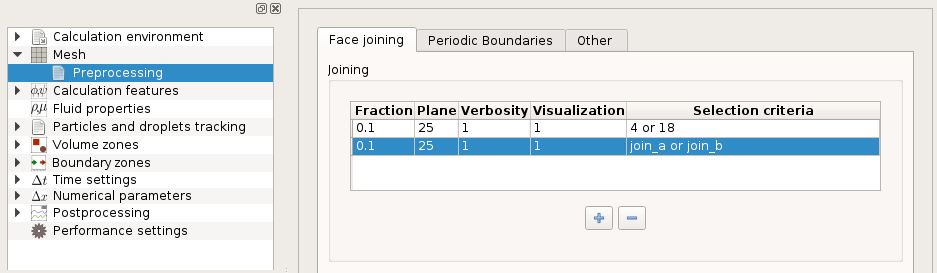
\includegraphics[width=15cm]{gui_mesh_join}
\caption{Conformal or non-conformal joining}
\label{fig:joining}
\end{center}
\end{figure}
%
For a simple mesh, it is rarely useful to specify strict face selection
criteria, as joining is sufficiently automated to detect which faces
may actually be joined. For a more complex mesh, or a mesh with thin
walls which we want to avoid transforming into interior faces, it is
recommended to filter boundary faces that may be joined by using
face selection criteria. This has the
additional advantage of reducing the number of faces to test for
in the intersection/overlap search, and thus reduced to time
required by the joining algorithm.

One may also modify tolerance criteria using 2 options:

\noindent
\begin{tabular}[top]{p{3.0cm}%
                     >{\PreserveBackslash\raggedright\hspace{0pt}}p{12.0cm}}
\texttt{fraction} $r$  &
assigns value $r$ (where $0 < r < 0,49$) to the maximum
intersection distance multiplier ($0,1$ by default). The maximum
intersection distance for a given vertex is based on the length of
the shortest incident edge, multiplied by $r$. The maximum intersection
at a given point along an edge is interpolated from that at its
vertices, as shown on the left of figure \ref{fig_join_tolerance}; \\
\texttt{lane} $c$ &
assigns the maximum angle between normals for two faces to be
considered coplanar ($25$\degresC by default);
this parameter is used in the second stage of the algorithm, to
reconstruct conforming faces, as shown on the right of figure
\ref{fig_join_tolerance}.\\
\end{tabular}

\begin{figure}[!hp]
\centerline{
\includegraphics*[width=14cm]{join_tolerance}}
\caption{Maximum intersection tolerance and faces normal angle
\label{fig_join_tolerance}}
\end{figure}

In practice, we are sometimes led to increase the maximum intersection
distance multiplier to $0.2$ or even $0.3$ when joining curved surfaces,
so that all intersection are detected. As this influences merging
of vertices and thus simplification of reconstructed faces, but also
deformation of ``lateral'' faces, it is recommended only to modify it
if necessary. As for the \texttt{plane} parameter, its use has
only been necessary on a few meshes up to now, and always in the
sense of reducing the tolerance so that face reconstruction does not
try to generate faces from initial faces on different surfaces.

\subsubsection{Periodicity\label{sec:optpcs:period}}

Handling of periodicity is based on an extension of conforming joining,
as shown on figure \ref{fig_join_periodic}. It is thus not necessary
for the periodic faces to be conforming (though it usually leads to better
mesh quality). All options relative to conforming joining of
non-conforming faces also apply to periodicity. Note also that
once pre-processed, 2 periodic faces have the same orientation
(possibly adjusted by periodicity of rotation).

This operation can also be performed by the solver and specified
either using the GUI or the \texttt{cs\_user\_periodicity} function.

\begin{figure}[!hp]
\centerline{
\includegraphics*[height=8cm]{join_periodic}}
\caption{Matching of periodic faces
\label{fig_join_periodic}}
\end{figure}

As with joining, it is recommended to filter boundary faces to process
using a selection criterion. As many periodicities may be built as desired,
as long as boundary faces are present. One a periodicity is handled,
faces having periodic matches do not appear as boundary faces, but as
interior faces, and are thus not available anymore for other
periodicities.

%==================================
\subsubsection{Parameters for conforming or non-conforming mesh joinings}
%==================================

The setting of these parameters is done in the user subroutine \texttt{cs\_user\_join} (called once). The user can specify the parameters used for the joining of different meshes. Below is given the list of the standard parameters which can me modified:
\begin{list}{-}{}
\item \texttt{fract}: the initial tolerance radius associated to each vertex is equal to the lenght of the shortest incident edge, multiplied by this fraction,
\item \texttt{plane}: when subdividing faces, 2 faces are considered coplanar and may be joined if the angle between their unit normals (in degree) does not exceed this parameter,
\item \texttt{iwarnj}: the associated verbosity level (debug level if over 3).
\end{list}
In the call of the function \texttt{cs\_join\_add}, a selection criteria for
mesh faces to be joined is specified.
The list of advanced modifiable parameters is given below:
\begin{list}{-}{}
\item \texttt{mtf}: a merge tolerance factor, used to locally modify the tolerance associated to each vertex before the merge step. Depending on its value four scenarii are possible:
\begin{list}{$\rightarrow$}{}
\item if $mtf=0$, no vertex merge
\item if $mtf<1$, the vertex merge is more strict. It may increase the number of tolerance reduction and therfore define smaller subset of vertices to merge together but it can drive to loose intersections.
\item if $mtf=1$, no change occurs
\item if $mtf>1$, the vertex merge is less strict. The subset of vertices able to merge is greater.
\end{list}
\item \texttt{pmf}: a pre-merge factor. This parameter is used to define a limit under which two vertices are merged before the merge step,
\item \texttt{tcm}: a tolerance computation mode. If its value is:
\begin{list}{$\rightarrow$}{}
\item 1 (default), the tolerance is the minimal edge length related to a vertex, multiplied by a fraction.
\item 2, the tolerance is computed like for 1 with, in addition, the multiplication by a coefficient equal to the maximum between $sin(e1)$ and $sin(e2)$; where $e1$ and $e2$ are two edges sharing the same vertex V for which we want to compute the tolerance.
\item 11, it is the same as 1 but taking into account only the selected faces.
\item 12, it is the same as 2 but taking into account only the selected faces.
\end{list}
\item \texttt{icm}: the intersection computation mode. If its value is:
\begin{list}{$\rightarrow$}{}
\item 1 (default), the original algorithm is used. Care should taken to clip the intersection on an extremity.
\item 2, a new intersection algorithm is used. Caution should be used to avoid to clip the intersection on an extremity.
\end{list}
\item \texttt{maxbrk}: defines the maximum number of equivalence breaks which is enabled during the merge step,
\item \texttt{maxsf}: defines the maximum number of sub-faces used when splitting a selected face
\end{list}
%
The followings are advanced parameters used in the search algorithm for face intersections between selected faces (octree structure). They are useful in case of memory limitation:
\begin{list}{-}{}
\item \texttt{tml}: the tree maximum level is the deepest level reachable during the tree building,
\item \texttt{tmb}: the tree maximum boxes is the maximum number of bounding boxes (BB) which can be linked to a leaf of the tree (not necessary true for the deepest level),
\item \texttt{tmr}: the tree maximum ratio. The building of the tree structure stops when the number of bounding boxes is superior to the product of \texttt{tmr} with the number of faces to locate. This is an efficient parameter to reduce memory consumption.
\end{list}
The call to the subroutine '\texttt{setajp}' returns the value of these parameters.

%==================================
\subsubsection{Parameters for the periodicity}
%==================================

Periodicities can be set directly in the Graphical User Interface (GUI) or using the user subroutine \texttt{cs\_user\_periodicity} (called when once during the calculation initialisation). In the GUI, the user can choose between 3 types of periodicities: translation, rotation, or mixed (see fig. \ref{fig:periodicities}).
Then specific parameters must be set.

\begin{figure}[!h]
\begin{center}
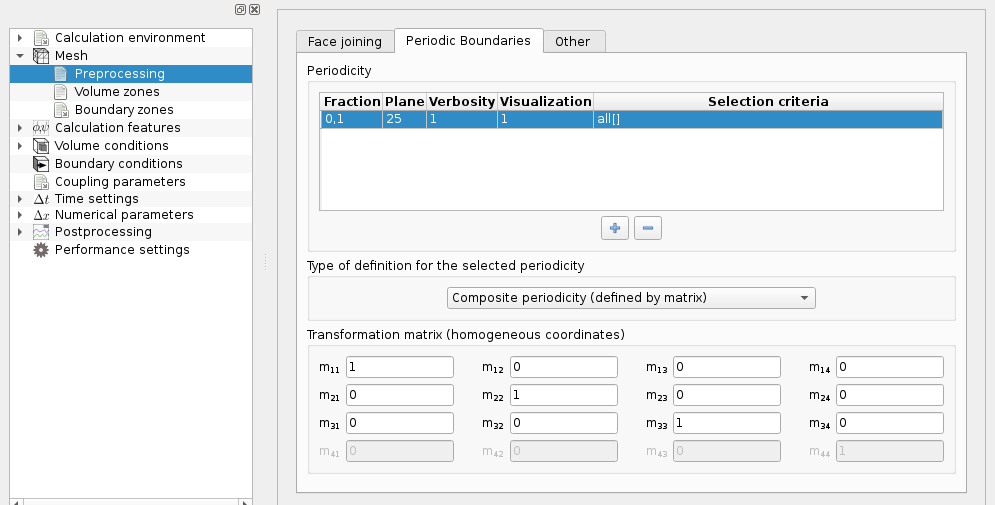
\includegraphics[width=14cm]{gui_mesh_periodicity}
\caption{Periodicity}
\label{fig:periodicities}
\end{center}
\end{figure}

\texttt{cs\_user\_periodicity} can be used instead of the GUI, it allows also the user to specify the parameters used to set periodicities and gives access to more advanced parameters. Below is given the list of the main parameters which can me modified:
\begin{list}{-}{}
\item \texttt{fract}: the initial tolerance radius associated to each vertex is equal to the lenght of the shortest incident edge, multiplied by this fraction,
\item \texttt{plane}. When subdividing faces, 2 faces are considered as coplanar and may be joined if the angle between their unit normals (in degree) does not exceed this parameter,
\item \texttt{iwarnj}: the associated verbosity level (debug level if over 3).
\end{list}
The second part of the subroutine is used to define the periodic transformations. The user provides in the subroutine '\texttt{defpro}' the reference of the mesh the transformation applies to, as well as:
\begin{list}{-}{}
\item the translation vector, if a periodicity of translation is used,
\item the axis, the angle of rotation, and an invariant point if a periodicity of rotation is used,
\item an homogeneous matrix if a general transformation is used.
\end{list}
In addition, the user can modify advanced parameters in case problems occur during the joining step, or to get a better mesh quality:
\begin{list}{-}{}
\item \texttt{mtf}: a merge tolerance factor, used to locally modify the tolerance associated to each vertex before the merge step. Depending on its value four scenarii are possible:
\begin{list}{$\rightarrow$}{}
\item if $mtf=0$, there is no vertex merge.
\item if $mtf<1$, the vertex merge is more strict. It may increase the number of tolerance reduction and therfore define smaller subset of vertices to merge together, but it can drive to loose intersections.
\item if $mtf=1$, no changes occur.
\item if $mtf>1$, the vertex merge is less strict. The subset of vertices able to merge is greater.
\end{list}
\item \texttt{pmf}: a pre-merge factor. This parameter is used to define a limit under which two vertices are merged before the merge step,
\item \texttt{tcm}: a tolerance computation mode. If its value is:
\begin{list}{$\rightarrow$}{}
\item 1 (default), the tolerance is the minimal edge length related to a vertex, multiplied by a fraction.
\item 2, the tolerance is computed like for 1 with, in addition, the multiplication by a coefficient equal to the maximum between $sin(e1)$ and $sin(e2)$, where $e1$ and $e2$ are two edges sharing the same vertex V for which we want to compute the tolerance.
\item 11, it is the same as 1 but taking into account only the selected faces.
\item 12, it is the same as 2 but taking into account only the selected faces.
\end{list}
\item \texttt{icm}: the intersection computation mode. If its value is:
\begin{list}{$\rightarrow$}{}
\item 1 (default), the original algorithm is used. Care should taken to clip the intersection on an extremity.
\item 2, a new intersection algorithm is used. Caution should be used to avoid to clip the intersection on an extremity.
\end{list}
\item \texttt{maxbrk}: defines the maximum number of equivalence breaks which are enabled during the merge step,
\item \texttt{maxsf}: defines the maximum number of sub-faces used when splitting a selected face
\end{list}
%
The following are advanced parameters used in the search algorithm for face intersections between selected faces (octree structure). There are useful in case of memory limitation:
\begin{list}{-}{}
\item \texttt{tml}: the tree maximum level is the deepest level reachable during the tree building
\item \texttt{tmb}: the tree maximum boxes is the maximum number of bounding boxes (BB) which can be linked to a leaf of the tree (not necessary true for the deepest level)
\item \texttt{tmr}: the tree maximum ratio. The building of the tree structure stops when the number of bounding boxes is superior than the product of \texttt{tmr} with the number of faces to locate. This is an efficient parameter to reduce memory consumption.
\end{list}
The call to the routine '\texttt{setapp}' returns the value of these parameters.

%==================================
\subsubsection{Modification of the mesh geometry}
%==================================
\noindent
\textit{Subroutines called only during the calculation initialisation.}

The user subroutine \texttt{cs\_user\_mesh\_input} allows a detailed
selection of imported meshes read, reading files multiple times,
applying geometric transformations, and renaming groups.

The user subroutine \texttt{cs\_user\_mesh\_modify} may be used
for advanced modification of the main \texttt{cs\_mesh\_t}} structure.

{\em WARNING: Caution must be exercised when using this subroutine
along with periodicity. Indeed, the periodicity parameters are not
updated accordingly, meaning that the periodicity may be unadapted
after one changes the mesh vertex coordinates. It is particularly
true when one rescales the mesh. Rescaling should thus be done
in a separate run, before defining periodicity.}

The user subroutine \texttt{cs\_user\_mesh\_thinwall} allows
insertion of thin walls in the calculation mesh. Currently, this
subroutine simply transforms the selected internal faces into boundary
faces, on which boundary conditions can (and must) be applied.

Faces on each side of a thin wall will share the same vertices,
so postprocessing of the main volume mesh may not show the
inserted walls, though they will appear in the main boundary
output mesh.

%==================================
\subsection{Mesh smoothing utilities}
%==================================
\noindent
\textit{Subroutine called only during the calculation initialisation.}

The smoothing utilities may be useful when the calculation mesh has local
defects. 
The principle of smoothers is to mitigate the local defects by averaging
the mesh quality. This procedure can help for the calculus robustness or/and 
results quality.

The user subroutine \texttt{cs\_user\_mesh\_smoothe} allows to use different
smoothing functions detailled below.

{\em WARNING 1: Caution must be exercised when using this subroutine
along with periodicity. Indeed, the periodicity parameters are not
currently updated accordingly, meaning that the periodicity may be
unadapted after one changes the mesh vertex coordinates. It is particularly
true when one rescales the mesh. Rescaling should thus be done
in a separate run, before defining periodicity.}

{\em WARNING 2: Caution must be exercised when using smoothing utilities
because the geometry may be modified. In order to preserve geometry,
the function} \texttt{cs\_mesh\_smoother\_fix\_by\_feature} {\em allows to 
fix by a feature angle criterion the mobility of boundary vertices.}

\subsubsection{Fix by feature}
The vertex normals are defined by the average of the normals of the
faces sharing the vertex.
The feature angle between a vertex and one of its adjacent faces is defined
by the angle between the vertex normal and the face normal.

This function sets a vertex if one of its feature angles is less than
$cos(\theta)$ where $\theta$ is the maximum feature angle (in degrees)
defined by the user.
In fact, if $\theta = 0^{\circ}$ all boundary vertices will be fixed, and 
if $\theta = 90^{\circ}$ all boundary vertices will be free.

Fixing all boundary vertices ensures the geometry is preserved, but reduces
the smoothing algorithm's effectiveness.

\subsubsection{Warped faces smoother}

The function \texttt{cs\_mesh\_smoother\_unwarp} allows to reduce face warping
in the calculation mesh.

Be aware that, in some cases, this algorithm may degrade other mesh quality 
criteria.

%==================================
\section{Partitioning for parallel runs\label{sec:parall}}
%==================================

Graph partitioning (using one of the optional \metis or
\scotch libraries) is done using a secondary executable,\\
\texttt{cs\_partition},
which reads the file produced by the \pcs and builds one or
several ``cell $\rightarrow$ domain'' distribution files, named
{\tt domain\_number\_\it{p}} for a partitioning on $p$ sub-domains.

This separation leads to extra work for the Kernel, which must
redistribute data read in {\tt mesh\_input}
based on the associated partitioning, but avoids requiring
re-running the \pcs whenever running on a different number of
processors.

Without partitioning (for example if neither \metis nor
\scotch is available, or the partitioner has not been run
for the required number of sub-domains), the Kernel will
use a built-in partitioning using a space-filling curve
(Z-curve) technique. This usually leads to partitionings
of lower quality than with graph partitioning, but parallel
performance remains reasonable.

\subsection{Options\label{sec:optcmd:parall}}

To list the partitioner's options, use the following command:
{\tt cs\_partition~-h} 

We provide the list of required partitionings an optionally additional
options. For example, to simulate a partitioning for calculations on
64 and 128 processes with no output, we may use the following command:

\texttt{cs\_partition 64 128 --no-write}

\subsubsection{Ignore periodicity\label{sec:optcmdpart:noperiod}}

By default, face periodicity relations are taken into account when building
the ``cell $\rightarrow$ cell'' connectivity graph used for partitioning.
This allows better partitioning optimization, but increases the probability
of having groups of cells at opposite sides of the domain in a same
sub-domain. This is not an issue for standard calculations, but may
degrade performance of search algorithms based on bounding boxes.
It is thus possible to ignore periodicity when partitioning a mesh
using the \texttt{--no-perio} option.

Note that nothing guarantees that a graph partitioner will not place
disjoint cells in the same sub-domain independently of this option,
but this behavior is rare.

\subsubsection{Partitioner choice\label{sec:optpart:partlib}}

If the Partitioner has been configured with both \metis and
\scotch libaries, using the \texttt{--metis} or \texttt{--scotch}
option allows choosing between either library. By default, \emph{metis} is
used if both choices are available.

\subsubsection{Simulation mode\label{sec:optpart:nowrite}}

Using the \texttt{--no-write} option, we can tell the partitioner
not to output a {\tt domain\_number\_\it{p}} file.
Partitioning is thus computed, but not saved.

\subsubsection{Environment variables\label{sec:optpart:envvar}}

\envvar{CS\_PARTITION\_MEM\_LOG}

Allows defining a file name in which memory allocations, reallocations,
and frees will be logged.


%==================================
\section{Basic modelling setup}
%==================================

%==================================
\subsection{Initialisation of the main parameters}
%==================================

This operation is done in the Graphical User Interface (GUI) or by using the user subroutine \texttt{usini1}.
In the GUI, the initialisation is performed by filling the parameters displayed in Figs. \ref{fig:6_GUI} to \ref{fig:28_GUI}. If the option 'Mobile mesh' is activated in Fig. \ref{fig:6_GUI}, please see Section \ref{sec:ALE} for more details. In fig. \ref{fig:11_GUI}, the equivalent initialisations occur in the subroutine \texttt{usiniv} when the GUI is not used.
The headings filled for the initialisation are the followings:
\begin{list}{-}{}
\item Thermophysical model options: ALE mobile mesh,
      turbulence model, thermal model, see figs. \ref{fig:6_GUI} to \ref{fig:8_GUI}.
\item Additional scalars: definition, initialisation of the scalars, and physical characteristics, see figs. \ref{fig:11_GUI} and \ref{fig:12_GUI}. In fig. \ref{fig:12_GUI}, the initial values are given in the subroutine \texttt{usiniv} if the GUI is not used, see Section \ref{sec:usiniv}.
\item Physical properties: reference pressure, fluid characteristics, gravity, see figs. \ref{fig:13_GUI} to \ref{fig:15_GUI}. If non-constant values are used for the fluid properties, and if the GUI is not used, see Section \ref{sec:usphyv}.
\item Numerical parameters: number and type of time steps, and advanced parameters for the numerical solution of the equations, see figs. \ref{fig:21_GUI} to \ref{fig:23_GUI}.
\item Calculation control: parameters related to the time averages, the time step, the
      locations of the probes where some variables will be monitored over time
      (if the GUI is not used, this information is specified in Section
      \ref{sec:usiniv}), the definition of the frequency of the outputs in the calculation
      listing, the postprocessing output writer frequency and format options, and
      the postprocessing output meshes and variables selection, see
      figs. \ref{fig:24_GUI}, \ref{gui_output_log}, \ref{gui_output_writers},
      and \ref{gui_output_meshes}. The item ``Profiles'' allows to save, with a
      frequency defined by the user, 1D profiles on an axis defined by two
      points, see fig. \ref{fig:26_GUI}.
\end{list}

\begin{figure}[!ht]
\begin{center}
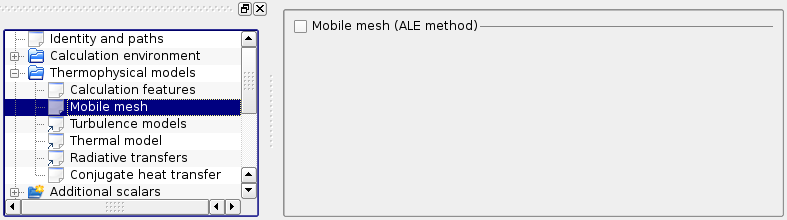
\includegraphics[width=13cm]{gui_mobile_mesh}
\caption{Mobile mesh option}
\label{fig:6_GUI}
\end{center}
\end{figure}

\begin{figure}[!ht]
\begin{center}
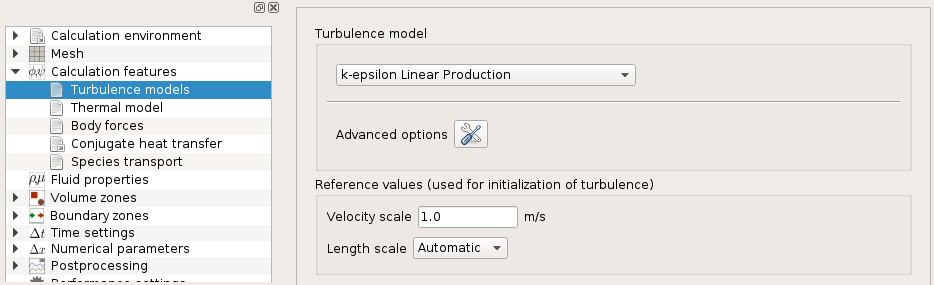
\includegraphics[width=13cm]{gui_turbulence_models}
\caption{Turbulence model selection}
\label{fig:7_GUI}
\end{center}
\end{figure}

\begin{figure}[!ht]
\begin{center}
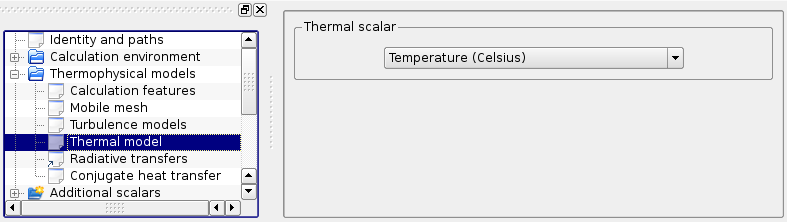
\includegraphics[width=13cm]{gui_thermal_scalar}
\caption{Thermal scalar selection}
\label{fig:8_GUI}
\end{center}
\end{figure}

\begin{figure}[!ht]
\begin{center}
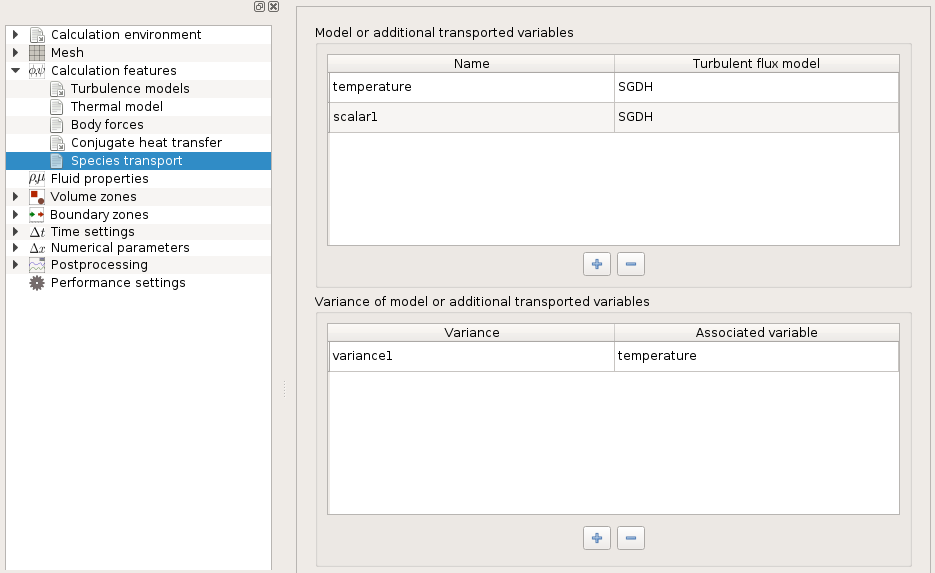
\includegraphics[width=13cm]{gui_user_scal_def_init}
\caption{Definition and initialisation of the scalars}
\label{fig:11_GUI}
\end{center}
\end{figure}

\begin{figure}[!ht]
\begin{center}
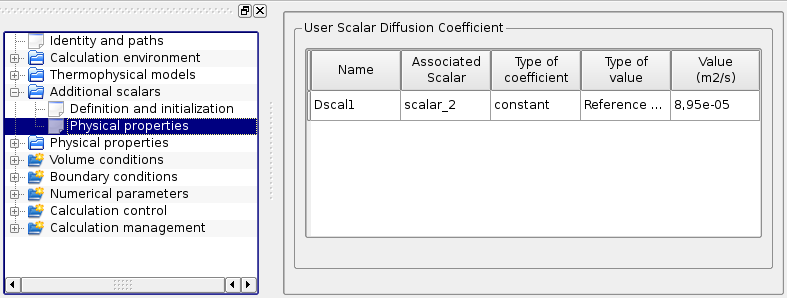
\includegraphics[width=13cm]{gui_user_scal_phys_props}
\caption{Associated physical properties of the scalars}
\label{fig:12_GUI}
\end{center}
\end{figure}

\begin{figure}[!ht]
\begin{center}
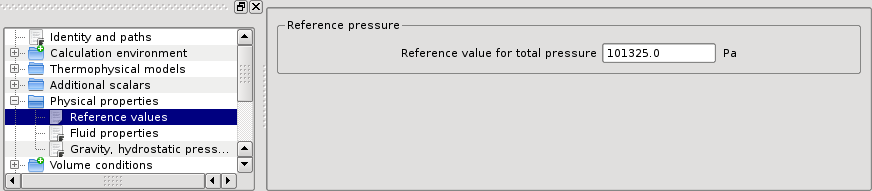
\includegraphics[width=13cm]{gui_phys_prop_ref_pressure}
\caption{Setting of the reference pressure}
\label{fig:13_GUI}
\end{center}
\end{figure}

\begin{figure}[!ht]
\begin{center}
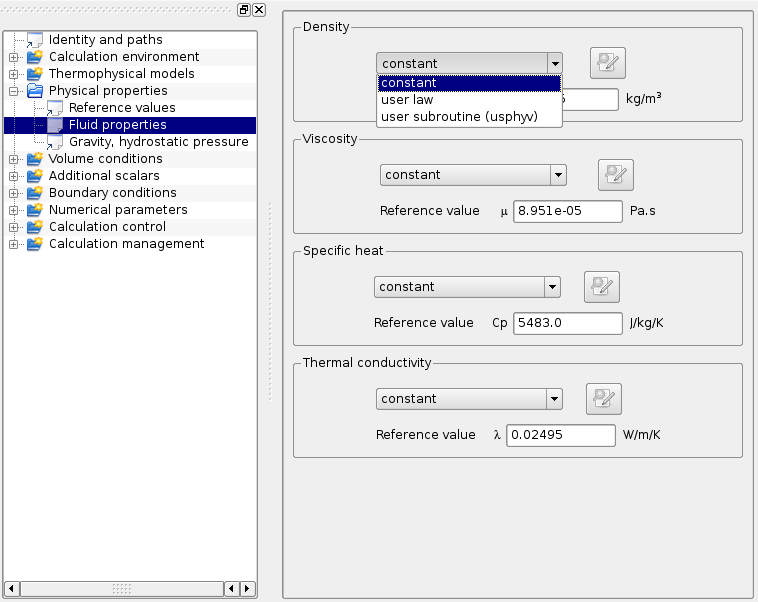
\includegraphics[width=13cm]{gui_fluid_props}
\caption{Fluid properties}
\label{fig:14_GUI}
\end{center}
\end{figure}

\begin{figure}[!ht]
\begin{center}
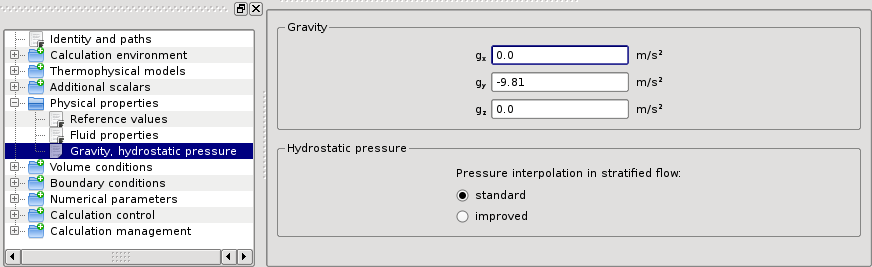
\includegraphics[width=13cm]{gui_gravity_hyd_pressure}
\caption{Settings of the gravity and of the hydrostatic pressure}
\label{fig:15_GUI}
\end{center}
\end{figure}

\begin{figure}[!ht]
\begin{center}
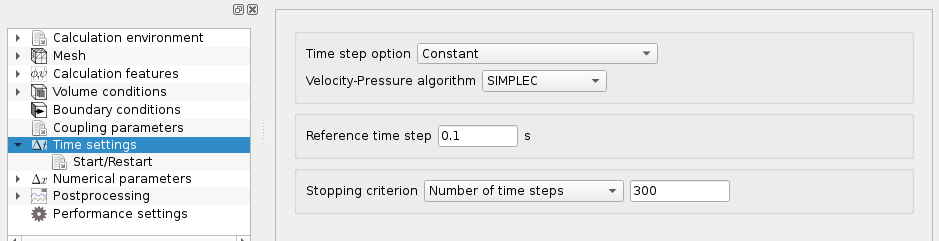
\includegraphics[width=13cm]{gui_time_step}
\caption{Time step settings}
\label{fig:21_GUI}
\end{center}
\end{figure}

\begin{figure}[!ht]
\begin{center}
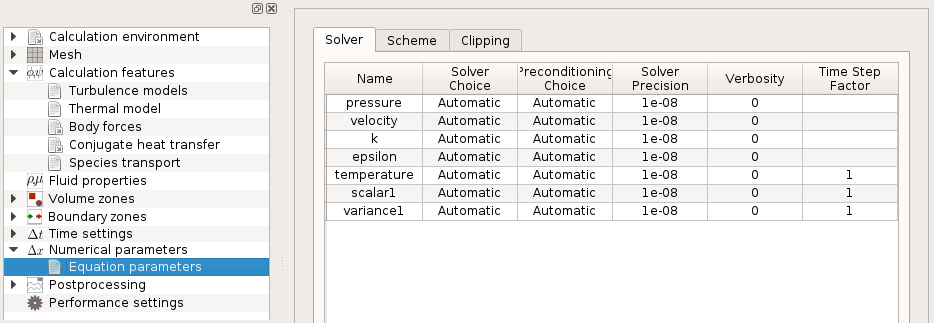
\includegraphics[width=13cm]{gui_numerical_parameters}
\caption{Numerical parameters for the main variables resolution}
\label{fig:22_GUI}
\end{center}
\end{figure}

\begin{figure}[!ht]
\begin{center}
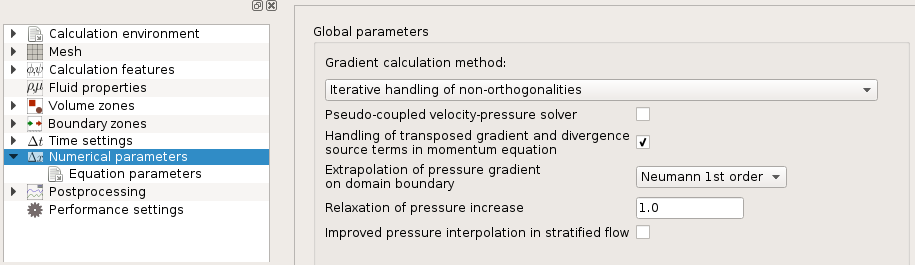
\includegraphics[width=13cm]{gui_global_res_parameters}
\caption{Global resolution parameters}
\label{fig:23_GUI}
\end{center}
\end{figure}

\begin{figure}[!ht]
\begin{center}
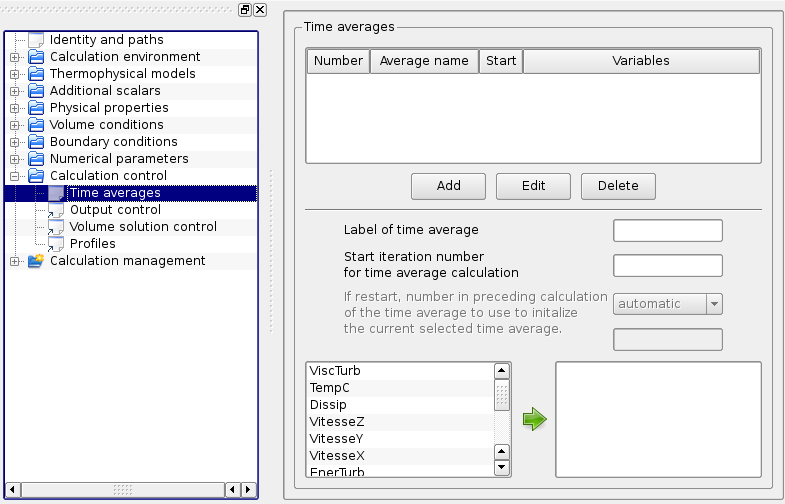
\includegraphics[width=13cm]{gui_time_averages}
\caption{Management of time averaged variables}
\label{fig:24_GUI}
\end{center}
\end{figure}

\begin{figure}[!ht]
\begin{center}
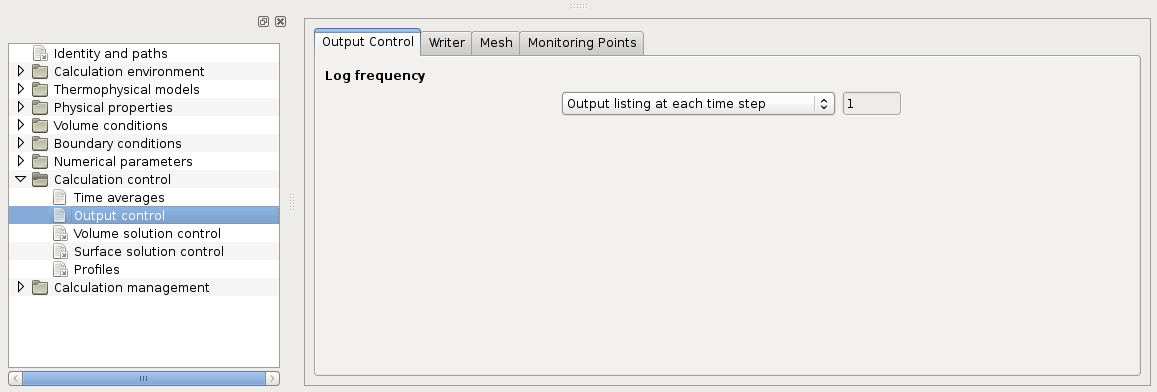
\includegraphics[width=13cm]{gui_output_log}
\caption{Parameters of chronological logging options}
\label{gui_output_log}
\end{center}
\end{figure}

\begin{figure}[!ht]
\begin{center}
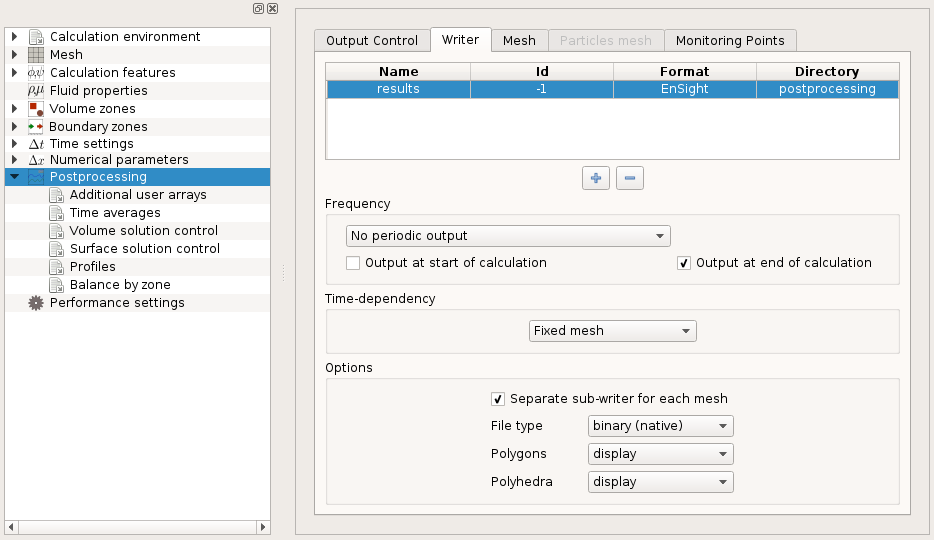
\includegraphics[width=13cm]{gui_output_writers}
\caption{Management of postprocessing writers}
\label{gui_output_writers}
\end{center}
\end{figure}

\begin{figure}[!ht]
\begin{center}
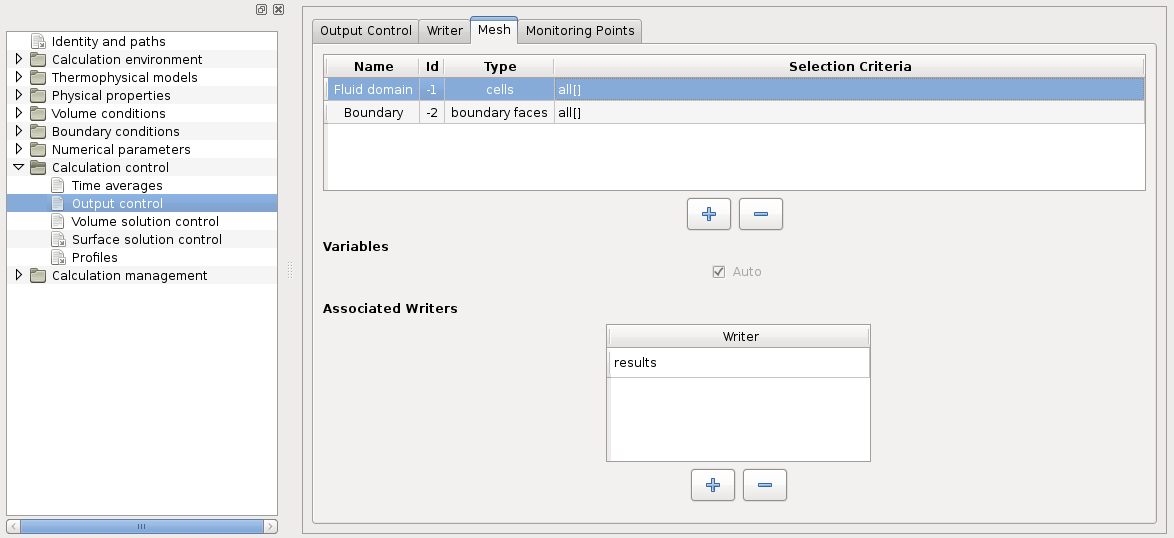
\includegraphics[width=13cm]{gui_output_meshes}
\caption{Management of postprocessing meshes}
\label{gui_output_meshes}
\end{center}
\end{figure}

\begin{figure}[!ht]
\begin{center}
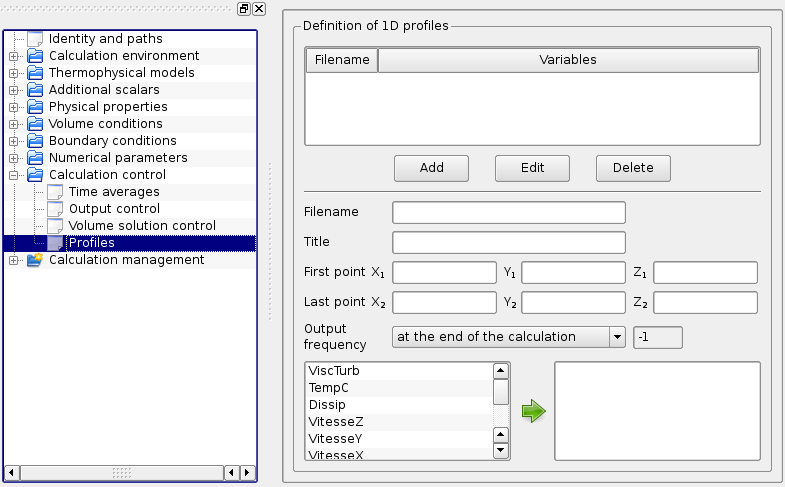
\includegraphics[width=13cm]{gui_output_1d_profiles}
\caption{Management of 1D profiles of the solution}
\label{fig:26_GUI}
\end{center}
\end{figure}

In the case of a calculation launched using the interface, the subroutine \texttt{usini1} is only
used to modify high-level parameters which can not be managed by the
interface. In the case of a code utilisation without interface, this
subroutine is compulsory and all the headings must be completed. \texttt{usini1} is used to indicate the value of different calculation
basic parameters: constant and uniform physical values, parameters of
numerical schemes, input-output management...\\
It is called only during the calculation initialisation.

For more details about the different parameters, please refer to the key
word list (\S\ref{prg_motscles}).

\texttt{usini1} is in fact constituted of 6 seperate subroutines:  \texttt{usipph},
 \texttt{usinsc}, \texttt{usipsc}, \texttt{usipgl},
\texttt{usipsu} and \texttt{usipes}. Each one controls various
 specific parameters. The key words which are not featured in the supplied example
can be provided by the user in \texttt{SRC/REFERENCE/base}; in this case,
understanding of the comments is required to add the key words in the appropriate
subroutine, it will ensure that the value
has been well defined). The modifiable parameters in each of the subroutines of
\texttt{usini1} are:

\begin{list}{$\bullet$}{}
\item \texttt{usipph}: \texttt{iturb} and \texttt{icp} (don't modify these
      parameters anywhere else)
\item \texttt{usinsc}: \texttt{nscaus} (don't modify these parameters anywhere
      else)
\item \texttt{usipsc}: \texttt{iscavr} and \texttt{ivisls} (don't modify these
      parameters anywhere else)
\item \texttt{usipgl}: \texttt{idtvar}, \texttt{ipucou}, \texttt{iphydr} and the
      parameters related to the error estimators (don't modify these parameters
      anywhere else).
\item \texttt{usipsu}: physical parameters of the calculation (thermal scalar, physical
      properties,...), numerical parameters (time steps, number of iterations, ...),
      definition of the time averages.
\item \texttt{usipes}: post-processing output parameters (periodicity, variable names,
      probe positions,...)
\end{list}

For more details on the different parameters, see the list of key words  (\S\ref{prg_motscles}).
 The names of the key words can also be seen in the help sections of the interface.

\minititre{Notes}
$\bullet\ $ The table \texttt{iscavr} is filled with the user scalars which represent the mean square fluctuations of another scalar amongst the list of the \texttt{nscaus} scalars (warning, this was not the case in version 1.0). For the other scalars, \texttt{iscavr} does not need to be completed (by default,
\texttt{iscavr(ii)}$\leqslant$0). For instance, if the scalar \texttt{jj}
represents the average of the square of the fluctuations of the scalar \texttt{kk},
the user must indicate \texttt{iscavr(jj)=kk}
(1$\leqslant$\texttt{kk}$\leqslant$\texttt{nscaus}).

\noindent
$\bullet\ $ When using the interface, only the
additional parameters (which can not be defined in the interface)
should appear in \texttt{usini1}. To spare the user the necessity to
delete the other parameters given as examples in the subroutine, the
setup program \texttt{code\_saturne~create} comments automatically all the
example lines of \texttt{usini1} with a code ``\texttt{!ex}''. The user
needs then only to remove comments at the lines which are useful for his
case. This function of
\texttt{code\_saturne~create} can be deactivated with
the option ``\texttt{--nogui}'' (useful if the user knows that he will not
use the interface).

\subsection{Selection of mesh inputs: \textmd{\texttt{cs\_user\_mesh\_input}}}
%==================================

\noindent
\textit{Subroutine called only during the calculation initialisation.}

This C function may be used to select which mesh input files
are read, and apply optional coordinate transformations or group renumberings
to them. By default, the input read is a file or directory named
\texttt{mesh\_input}, but if this function is used, any file may be selected,
and the same file may be read multiple times (applying a different
coordinate transformation each time).
All inputs read through this function are automatically concatenated, and
may be later joined using the mesh joining options.

Geometric transformations are defined using a homogeneous coordinates
transformation matrix. Such a matrix has 3 lines and 4 columns, with the
3 first columns describing a rotation/scaling factor, and the last column
describing a translation. A 4th line is implicit, containing zeroes
off-diagonal, and 1 on the diagonal. The advantages of this representation
is that any rotation/translation/scaling combination may be expressed
by matrix multiplication, while simple rotations or translations
may still be defined easily.

%==================================
%==================================
\subsection{Non-default variables initialisation} \label{sec:usiniv}
%==================================

The non-default variables initialisation is performed in the subroutine \texttt{usiniv} (called only during the calculation initialisation).\\ At the calculation beginning, the variables are initialised
automatically by the code. Velocities and scalars are set to 0 (or \texttt{scamax} or \texttt{scamin} if 0 is outside the acceptable
scalar variation range), and the turbulent variables are estimated from
\texttt{uref} and \texttt{almax}. \\
For the $k$ in $k-\varepsilon$, $R_{ij}-\varepsilon$, v2f or $k-\omega$
model:\\
{\texttt{rtp(iel,ikiph) = 1.5*(0.02*uref)**2}
(in $R_{ij}-\varepsilon$,  $R_{ij}=\frac{2}{3}k\delta_{ij}$)\\
For the $\varepsilon$ in $k-\varepsilon$, $R_{ij}-\varepsilon$ or v2f model:\\
\texttt{rtp(iel,ieiph) = rtp(iel,ikiph)**1.5*cmu/almax}\\
For $\omega$ in the $k-\omega$ model:\\
\texttt{rtp(iel,iomgip) = rtp(iel,ikiph)**0.5/almax}\\
For $\varphi$ and $\overline{f}$ in the v2f model:\\
\texttt{rtp(iel,iphiph) = 2/3}\\
\texttt{rtp(iel,ifbiph) = 0}

The subroutine \texttt{usiniv} allows if necessary to initialise certain
variables to values closer to their estimated final values, in order to
obtain a faster convergence.

This subroutine allows also to make a non-standard initialisation of
physical parameters (density, viscosity, ...), to impose a local
value of the time step, or to modify some parameters (time step,
variable specific heat, ...) in the case of a calculation restart.

\minititre{Note: value of the time step}
\begin{list}{-}{}
\item For calculations with constant and uniform time step
      (\texttt{idtvar}=0), the value of the time step is \texttt{dtref},
      given in the parametric file of the interface or \texttt{usini1}.
\item For calculations with a non-constant time step
      (\texttt{idtvar}=1 or 2) which is not a calculation restart,
      the value of \texttt{dtref} given in the parametric file of the interface
      or in \texttt{usini1} is used to initialise the time step.
\item For calculations with a non-constant time step
      (\texttt{idtvar}=1 or 2) which is a restart of a
      calculation whose time step type was different (for instance, restart
      using a variable time step of a calculation run using a constant time
      step), the value of \texttt{dtref}, given in the parametric file of the
      interface or in \texttt{usini1}, is used to initialise the time step.
\item For calculations with non-constant time step
      (\texttt{idtvar}=1 or 2) which is a restart of a
      calculation whose time step type was the same (for instance, restart with
      \texttt{idtvar}=1 of a calculation run with \texttt{idtvar}=1), the time
      step is read from the restart file and the value of \texttt{dtref} given
      in the parametric file of the interface, or in \texttt{usini1}, is not used.
\end{list}
It follows, that for a calculation with a non-constant time step (\texttt{idtvar}=1
or 2) which is a restart of a calculation in which
\texttt{idtvar} had the same value, \texttt{dtref} does not allow to modify the
time step. The user subroutine \texttt{usiniv} allows to modify the array
\texttt{dt} which contains the value of the time step read from the restart file
(array whose size is \texttt{ncelet}, defined at the cell centers whatever the
chosen time step type is).

{\em WARNING: to initialise the variables in the framework of a
specific physics module} (\texttt{nscapp.gt.0}), 
one of the subroutines
\texttt{usebui}, \texttt{usd3pi}, \texttt{uslwci} or \texttt{uscpiv} 
should be used (depending on the activated module) instead of \texttt{usiniv}.

%==================================
\subsection{Manage boundary conditions}
%==================================
The boundary conditions can be specified in the Graphical User Interface (GUI) under the heading ``Boundary conditions'' or in the user subroutine \texttt{usclim} called every time step. With the GUI, each region and the type of boundary condition associated to it are defined in fig. \ref{fig:19_GUI}. Then, the parameters of the boundary condition are specified in fig. \ref{fig:20_GUI}. The colors of the boundary faces may be read directly from a ``listing'' file created by the Preprocessor. This file can be generated directly by the interface under the heading ``Definition of boundary regions $\rightarrow$ Add from Preprocessor listing $\rightarrow$ import groups and references from Preprocessor listing'', see fig. \ref{fig:19_GUI}.
%
\begin{figure}[!ht]
\begin{center}
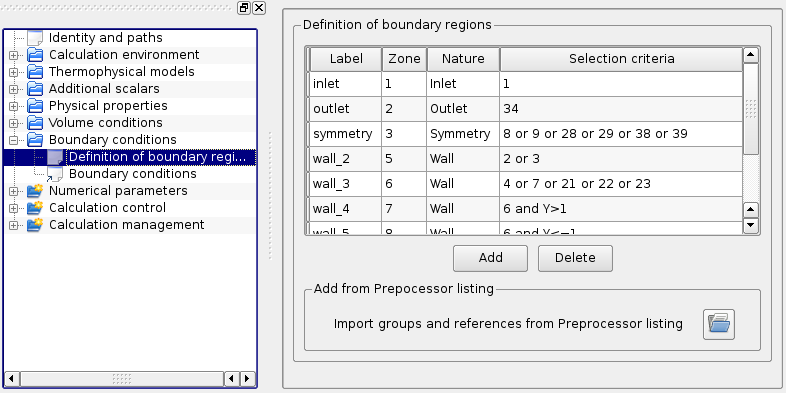
\includegraphics[width=13cm]{gui_bc_regions}
\caption{Definition of the boundary conditions}
\label{fig:19_GUI}
\end{center}
\end{figure}
%
\begin{figure}[!ht]
\begin{center}
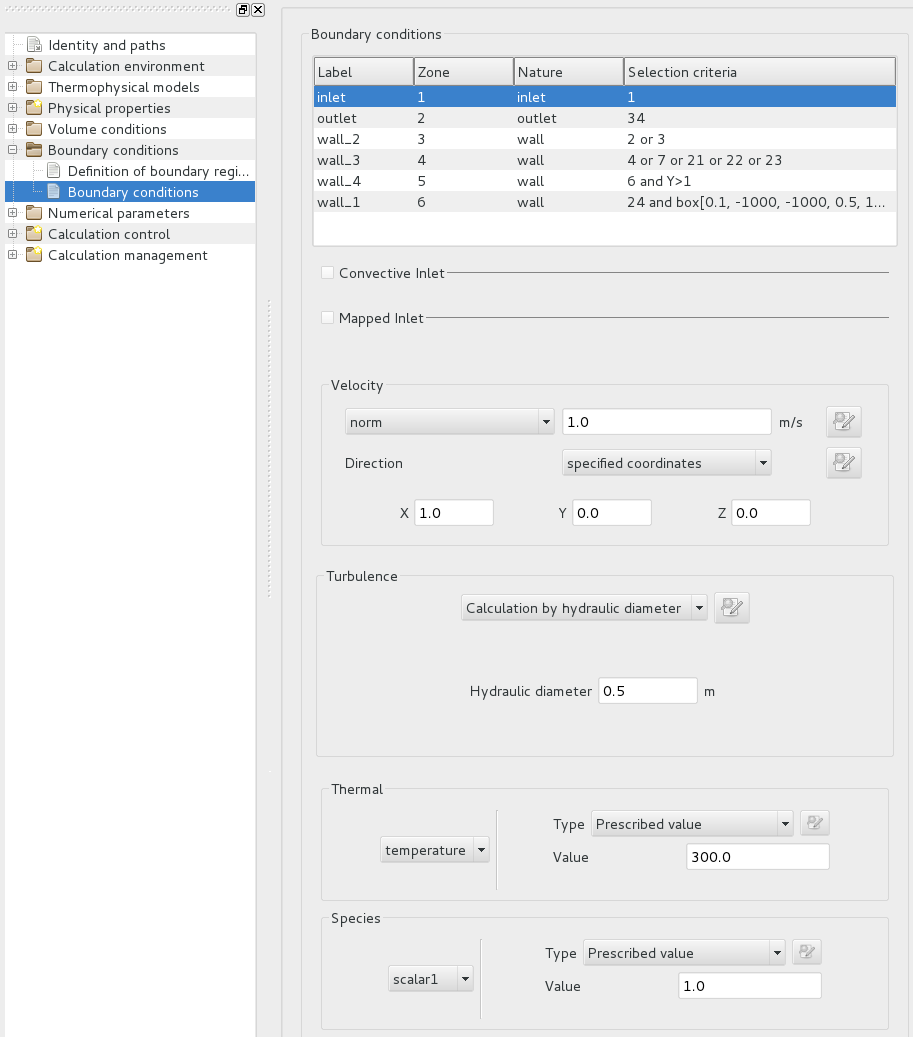
\includegraphics[width=13cm]{gui_bc_parameters}
\caption{Parameters of the boundary conditions}
\label{fig:20_GUI}
\end{center}
\end{figure}

\texttt{usclim} is the second compulsory subroutine for every calculation launched
without interface (except in the case of specific physics where the
corresponding boundary condition user subroutine must be used)  \\
When the subroutine is used, \texttt{usclim} is used to define complex
boundary conditions (input profiles, conditions varying in time, ...)
which could not be specified by the means of the interface, and only these
need to be defined. In the case of a calculation launched without the
interface, all the boundary conditions must appear in \texttt{usclim}.\\
\texttt{usclim} is essentially constituted of loops on boundary
face subsets. Several sequences 
of \verb+call getfbr+ \verb+('criterion', nlelt, lstelt)+ (cf.
\S\ref{fvm_selector}) allow to select 
the boundary faces with respect to their group(s), their
color(s) or geometric criteria. If needed, geometric and
physical variables are also available to the user. These allow him
to select the boundary faces using other criteria.

For more details about the treatment of boundary conditions, the user
may refer to the theoretical and computer documentation \cite{theory} of
the subroutine \texttt{condli} (for wall conditions, see
\texttt{clptur}) (to access this document on a workstation, use
\mbox{\texttt{code\_saturne~info --guide theory}}).

From the user point of view, the boundary conditions are fully
defined by three arrays\footnote{except with Lagrangian}:
\texttt{itypfb(nfabor)}\index{\texttt{itypfb}},
\texttt{icodcl(nfabor,nvar)}\index{\texttt{icodcl}} and
\texttt{rcodcl(nfabor,nvar,3)}\index{\texttt{rcodcl}}.
\begin{list}{-}{}
\item \texttt{itypfb(ifac)} defines the type of the face \texttt{ifac}
      (input, wall, ...).
\item \texttt{icodcl(ifac,ivar)} defines the type of boundary
      condition for the variable \texttt{ivar} on the face \texttt{ifac}
      (Dirichlet, flux ...).
\item \texttt{rcodcl(ifac,ivar,.)} gives the numerical values associated with the
      type of boundary condition (value of the Dirichlet, of the flux ...).
\end{list}

In the case of standard boundary conditions (see
\S\ref{prg_clstandard}), it is sufficient to complete \texttt{itypfb(ifac)} and
parts of the array \texttt{rcodcl}; the array \texttt{icodcl} and most of \texttt{rcodcl} are filled automatically. For non-standard boundary
conditions (see \S\ref{prg_clnonstandard}), the arrays \texttt{icodcl} and
\texttt{rcodcl} must be fully completed.

%==================================
\subsubsection{Coding of standard boundary conditions}
%==================================
\label{prg_clstandard}%
The standard key words used by the indicator \texttt{itypfb} are:
\texttt{ientre\index{ientre}}, \texttt{iparoi\index{iparoi}},
\texttt{iparug\index{iparug}}, \texttt{isymet\index{isymet}},
\texttt{isolib\index{isolib}} and \texttt{iindef\index{iindef}}.

\begin{list}{$\bullet$}{}
\item If \texttt{itypfb=ientre}: inlet face.

\begin{list}{$\rightarrow$}{}
\item Zero-flux condition for pressure and Dirichlet condition for all
      other variables. The value of the Dirichlet must be given in
      \texttt{rcodcl(ifac,ivar,1)} for every value of \texttt{ivar}, except for
      \texttt{ivar=ipr}. The other values of \texttt{rcodcl} and
      \texttt{icodcl} are filled automatically.
\end{list}

\item If \texttt{itypfb=iparoi}: smooth solid wall face, impermeable and with friction.

\begin{list}{$\rightarrow$}{}
\item the potential sliding wall velocity of the face is
      found in \texttt{rcodcl(ifac,ivar,1)} (\texttt{ivar} being
      \texttt{iu}, \texttt{iv} or \texttt{iw)}. The initial
      values of \texttt{rcodcl(ifac,ivar,1)} are zero for
      the three velocity components (and therefore are to be specified
      only if the velocity is not equal to zero). \\
{\em WARNING: the wall sliding velocity must belong to the boundary face
      plane. For safety, the code only uses the projection of this
      velocity on the face. As a consequence, if the velocity specified
      by the user does not belong to the face plane, the wall sliding velocity really
      taken into account will be different.}

\item For scalars, two kinds of boundary conditions can be
      defined:
\begin{list}{$\rightsquigarrow$}{}
\item Imposed value at the wall. The user must write\\
\hspace*{1cm}\texttt{icodcl(ifac,ivar)}=5\\
\hspace*{1cm}\texttt{rcodcl(ifac,ivar,1)}=imposed value\\
\item Imposed flux at the wall. The user must write\\
\hspace*{1cm}\texttt{icodcl(ifac,ivar)}=3\\
\hspace*{1cm}\texttt{rcodcl(ifac,ivar,3)}=flux imposed value (depending on the variable, the user may refer to the case \texttt{icodcl}=3 of Section \ref{prg_clnonstandard} for the flux definition).
\item If the user does not fill these arrays, the default condition
      is zero flux.
\end{list}
\end{list}

\item If \texttt{itypfb=iparug}: rough solid wall face, impermeable and with friction.

\begin{list}{$\rightarrow$}{}
\item the eventual moving velocity of the wall tangent to the face is
      given by \texttt{rcodcl(ifac,ivar,1)} (\texttt{ivar} being
      \texttt{iu}, \texttt{iv} or \texttt{iw}). The initial
      value of \texttt{rcodcl(ifac,ivar,1)} is zero for
      the three velocity components (and therefore needs to be specified
      only in the case of the existence of a slipping velocity). \\
{\em WARNING: the wall moving velocity must be in the boundary face
      plane. By security, the code uses only the projection of this
      velocity on the face. As a consequence, if the velocity specified
      by the user is not in the face plane, the wall moving velocity really
      taken into account will be different.}
\item The dynamic roughness must be specified in \texttt{rcdocl(ifac,iu,3)}.
      The values of \texttt{rcdocl(ifac,iv,3)} and
      \texttt{rcdocl(ifac,iw,3)} are not used.
\item For scalars, two kinds of boundary conditions can be defined:
\begin{list}{$\rightsquigarrow$}{}
\item Imposed value at the wall. The user must write\\
\hspace*{1cm}\texttt{icodcl(ifac,ivar)}=6\\
\hspace*{1cm}\texttt{rcodcl(ifac,ivar,1)}=imposed value\\
\hspace*{1cm}\texttt{rcodcl(ifac,ivar,3)}=thermal roughness value\\
\item Imposed flux at the wall. The user must write\\
\hspace*{1cm}\texttt{icodcl(ifac,ivar)}=3\\
\hspace*{1cm}\texttt{rcodcl(ifac,ivar,3)}=flux imposed value (for the flux
      definition according to the variable, the user may refer to the
      case \texttt{icodcl}=3 of the paragraph \ref{prg_clnonstandard}).
\item If the user does not complete these arrays, the default condition
      is zero flux.
\end{list}
\end{list}
\item If \texttt{itypfb=isymet}: symmetry face (or wall without friction)
\begin{list}{$\rightarrow$}{}
\item Nothing to be writen in \texttt{icodcl} and  \texttt{rcodcl}.
\end{list}

\item If \texttt{itypfb=isolib}: free outlet face (or more precisely free 
      inlet/outlet with forced pressure)
\begin{list}{$\rightarrow$}{}
\item The pressure is always treated with a Dirichlet condition, calculated
      with the constraint $\displaystyle \frac{d}{dn}\left(\frac{dP}{d\tau}\right)=0$.
      The pressure is set to $P_0$ at the first \texttt{isolib} face met.
      The pressure calibration is always done on a single face, even if there are
      several outlets.
\item If the mass flow is coming in, the ``infinite'' velocity is retained
      and a Dirichlet condition for the scalars and the turbulent quantities is used
      (or zero-flux condition if no Dirichlet value has been specified).
\item If the mass flow is going out, zero-flux condition are set for the velocity,
      the scalars and the turbulent quantities.
\item Nothing is written in \texttt{icodcl} or \texttt{rcodcl} for the pressure or
      the velocity. An optional Dirichlet condition can be specified for the scalars
      and turbulent quantities.
\end{list}

\item If \texttt{itypfb=iindef}: undefined type face (non-standard case)
\begin{list}{$\rightarrow$}{}
\item Coding is done in a non-standard way by filling both arrays \texttt{rcodcl} and
      \texttt{icodcl} (see \S\ref{prg_clnonstandard}).
\end{list}
\end{list}

\minititre{Notes}
$\bullet\ $ Whatever is the value of the indicator \texttt{itypfb(ifac)}, if
the array \texttt{icodcl(ifac,ivar)} is modified by the user ({\em i.e.} filled
with a non-zero value), the code will not use the default
conditions for the variable \texttt{ivar} at the face \texttt{ifac}. It will
take into account only the values of \texttt{icodcl} and \texttt{rcodcl} provided by the
user (these arrays must then be fully completed, like in the non-standard case). \\
For instance, for a normal symmetry face where scalar 1 is associated with a
Dirichlet condition equal to 23.8 (with an infinite exchange
coefficient):\\
\hspace*{2cm}\texttt{itypfb(ifac)=isymet}\\
\hspace*{2cm}\texttt{icodcl(ifac,isca(1))=1}\\
\hspace*{2cm}\texttt{rcodcl(ifac,isca(1),1)=23.8}\\
(\texttt{rcodcl(ifac,isca(1),2)=rinfin} is the default value, therfore it is
not necessary to specify a value)\\
The boundary conditions for the other variables are remain automatically
defined.

\noindent
$\bullet\ $The user can define new types of boundary faces. He only needs to
choose a value $N$ and to fully specify the boundary conditions (see
\S\ref{prg_clnonstandard}). He must specify
\texttt{itypfb(ifac)}=$N$ where $N$ range is 1 to
\texttt{ntypmx\index{ntypmx}} (maximum number of boundary face types), and of
course different from the values \texttt{ientre}, \texttt{iparoi},
\texttt{iparug}, \texttt{isymet}, \texttt{isolib} and \texttt{iindef} (the values
of these variables are given in the file \texttt{paramx.h}). This allows to
easily isolate some boundary faces, in order for instance to calculate balances.

%==================================
\subsubsection{Coding of non-standard boundary conditions}
%==================================
\label{prg_clnonstandard}%
In the case a face does not correspond to a standard type, the user
must fill completely the arrays \texttt{itypfb}, \texttt{icodcl} and
\texttt{rcodcl}. \texttt{itypfb(ifac)} is then equal to \texttt{iindef}
or another value defined by the user (see note at the end of Section
\ref{prg_clstandard}). The arrays \texttt{icodcl} and \texttt{rcodcl}
must be filled as follows:

\begin{list}{$\bullet$}{}
\item If \texttt{icodcl(ifac,ivar)}=1: Dirichlet condition at the face
      \texttt{ifac} for the variable \texttt{ivar}.

\begin{list}{$\rightarrow$}{}
\item \texttt{rcodcl(ifac,ivar,1)} is the value of the variable \texttt{ivar}
      at the face \texttt{ifac}.

\item \texttt{rcodcl(ifac,ivar,2)} is the value of the exchange coefficient
      between the outside and the fluid for the variable \texttt{ivar}. An
      infinite value (\texttt{rcodcl(ifac,ivar,2)=rinfin}) indicates an
      ideal transfer between the outside and the fluid (default case).

\item \texttt{rcodcl(ifac,ivar,3)} is not used.

\item \texttt{rcodcl(ifac,ivar,1)} has the units of the variable
      \texttt{ivar}, {\em i.e.}:
\begin{list}{$\rightsquigarrow$}{}
\item $m/s$ for the velocity

\item $m^2/s^2$ for the Reynolds stress

\item $m^2/s^3$ for the dissipation

\item $Pa$ for the pressure

\item \degresC\ for the temperature

\item $J.kg^{-1}$ for the enthalpy

\item \degresC$^2$ for temperature fluctuations

\item $J^2.kg^{-2}$ for enthalpy fluctuations
\end{list}

\item \texttt{rcodcl(ifac,ivar,2)} has the following units (defined in such way that when multiplying the exchange coefficient by the variable, the
      given flux has the same units as the flux defined below when
      \texttt{icodcl=3)}:

\begin{list}{$\rightsquigarrow$}{}
\item $kg.m^{-2}.s^{-1}$ for the velocity

\item $kg.m^{-2}.s^{-1}$ for the Reynolds stress

\item $s.m^{-1}$ for the pressure

\item $W.m^{-2}.\mbox{\degresC}^{-1}$ for the temperature

\item $kg.m^{-2}.s^{-1}$ for the enthalpy
\end{list}

\end{list}

\item If \texttt{icodcl(ifac,ivar)=3}: flux condition at the face \texttt{ifac}
      for the variable \texttt{ivar}.

\begin{list}{$\rightarrow$}{}
\item \texttt{rcodcl(ifac,ivar,1)} and \texttt{rcodcl(ifac,ivar,2)} are not used.

\item \texttt{rcodcl(ifac,ivar,3)} is the flux value of \texttt{ivar} at the
      wall. This flux is negative if it is a source for the fluid. It corresponds to:
\begin{list}{$\rightsquigarrow$}{}
\item
$\displaystyle -C_p(\frac{\lambda_T}{C_p}+\frac{\mu_t}{\sigma_T})\grad T\cdot\vect{n}$ for a temperature (in $W/m^2$).

$\displaystyle -(\lambda_h+\frac{\mu_t}{\sigma_h})\grad h\cdot\vect{n}$
     for an enthalpy (in $W/m^2$).

$\displaystyle -(\lambda_\varphi+\frac{\mu_t}{\sigma_\varphi})\grad\varphi\cdot\vect{n}$ in the case of another scalar $\varphi$ (in $kg.m^{-2}.s^{-1}.[\varphi]$, where $[\varphi]$ are the units of $\varphi$).

\item $-\Delta t\ \grad P\cdot\vect{n}$ for the pressure (in $kg.m^{-2}.s^{-1}$).

\item $-(\mu+\mu_t)\grad U_i\cdot\vect{n}$ for a velocity component (in $kg.m^{-1}.s^{-2}$).

\item $-\mu\grad R_{ij}\cdot\vect{n}$ for a $R_{ij}$ tensor component (in $W/m^2$).
\end{list}

\end{list}

\item If \texttt{icodcl(ifac,ivar)}=4: symmetry condition, for the symmetry
      faces or wall faces without friction. This condition can only be
      used for velocity components ($\vect{U}\cdot\vect{n}=0$) and
      the $R_{ij}$ tensor components (for other variables, a zero-flux
      condition type is usually used).\\

\item If \texttt{icodcl(ifac,ivar)}=5: friction condition, for wall faces
      with friction. This condition can not be applied to the pressure.
\begin{list}{$\rightsquigarrow$}{}
\item For the velocity and (if necessary) the turbulent variables, the
      values at the wall are calculated from theoretical profiles. In
      the case of a sliding wall, the three components of the sliding
      velocity are given by (\texttt{rcodcl(ifac,iu,1)},
      \texttt{rcodcl(ifac,iv,1)}, and \texttt{rcodcl(ifac,iw,1)}).\\
{\em WARNING: the wall sliding velocity must belong to the boundary face
      plane. For safety, the code uses only the projection of this
      velocity on the face. Therefore, if the velocity vector specified
      by the user does not belong to the face plane, the wall sliding velocity really
      taken into account will be different.}

\item For other scalars, the condition \texttt{icodcl}=5 is similar to
      \texttt{icodcl=1}, but with a wall exchange coefficient calculated from a
      theoretical law. Therefore, the values of \texttt{rcodcl(ifac,ivar,1)} and
      \texttt{rcodcl(ifac,ivar,2)} must be specified: see \cite{theory}.
\end{list}

\item If \texttt{icodcl(ifac,ivar)}=6: friction condition, for the rough-wall faces
      with friction. This condition can not be used with the pressure.
\begin{list}{$\rightsquigarrow$}{}
\item For the velocity and (if necessary) the turbulent variables, the
      values at the wall are calculated from theoretical profiles. In
      the case of a sliding wall, the three components of the sliding
      velocity are given by (\texttt{rcodcl(ifac,iu,1)},
      \texttt{rcodcl(ifac,iv,1)}, and \texttt{rcodcl(ifac,iw,1)}).\\
{\em WARNING: the wall sliding velocity must belong to the boundary face
      plane. For safety, the code uses only the projection of this
      velocity on the face. Therefore, if the velocity vector specified
      by the user does not belong to the face plane, the wall sliding velocity really
      taken into account will be different.}\\
      The dynamic roughness height is given by \texttt{rcodcl(ifac,iu,3)} only.

\item For the other scalars, the condition \texttt{icodcl}=6 is similar to
      \texttt{icodcl}=1, but with a wall exchange coefficient calculated from a
      theoretical law. The values of \texttt{rcodcl(ifac,ivar,1)} and
      \texttt{rcodcl(ifac,ivar,2)} must therefore be specified: see \cite{theory}.
      The thermal roughness height is then given by \texttt{rcodcl(ifac,ivar,3)}.
\end{list}

\item If \texttt{icodcl(ifac,ivar)}=9: free outlet condition for the
      velocity. This condition is only applicable to velocity
      components.\\
If the mass flow at the face negative, this condition is equivalent
      to a zero-flux condition.\\
If the mass flow at the face is positive, the velocity at the face is set to zero (but not to the mass flow).\\
\texttt{rcodcl} is not used.

\end{list}

\minititre{Note}
$\bullet\ $A standard \texttt{isolib} outlet face amounts to a Dirichlet
condition (\texttt{icodcl}=1) for the pressure, a free outlet condition
(\texttt{icodcl}=9) for the velocity and a Dirichlet condition
(\texttt{icodcl}=1) if the user has specified a Dirichlet value or a zero-flux
condition (\texttt{icodcl}=3) for the other variables.\\

%==================================
\subsubsection{Checking of the boundary conditions}
%==================================

The code checks the main compatibilities between the boundary
conditions. In particular, the following rules must be respected: \\
$\bullet\ $On each face, the boundary conditions of the three velocity components must belong to the same type. The same is true for the components of the $R_{ij}$ tensor.\\
$\bullet\ $If the boundary conditions for the velocity belong to the
``sliding'' type (\texttt{icodcl}=4), the conditions for $R_{ij}$ must belong to
the ``symmetry'' type (\texttt{icodcl}=4), and vice versa.\\
$\bullet\ $If the boundary conditions for the velocity belong to the
``friction'' type (\texttt{icodcl}=5 or 6), the boundary conditions for the turbulent variables
must belong to the ``friction'' type, too.\\
$\bullet\ $If the boundary condition of a scalar belongs to the
``friction'' type, the boundary condition of the velocity must belong to
the ``friction'' type, too.

In case of mistakes, if the post-processing output is activated (which is the default setting),
a special error output, similar to the mesh format, is produced in order to help
correcting boundary condition definitions.

%==================================
\subsubsection{Sorting of the boundary faces}
%==================================

In the code, it may be necessary to have access to all the boundary
faces of a given type. To ease this kind of search, an array made of
sorted faces is automatically filled (and updated at each time step):
\texttt{itrifb(nfabor)\index{itrifb}}.\\
\texttt{ifac=itrifb(i)} is the number of the i$^{\text{th}}$  face of type
1.\\
\texttt{ifac=itrifb(i+n)} is the number of the i$^{\text{th}}$ face of type
2, if there are $n$ faces of type 1.\\
... etc.

Two auxiliary arrays of size \texttt{ntypmx} are also defined.\\
\texttt{idebty(ityp)\index{idebty}} is the index
corresponding to the first
face of type \texttt{ityp} in the array \texttt{itrifb}.\\
\texttt{ifinty(ityp)\index{ifinty}} is the index
corresponding to the last
face of type \texttt{ityp} in the array \texttt{itrifb}.

Therefore, a value \texttt{ifac0} found between \texttt{idebty(ityp)} and
\texttt{ifinty(ityp)} is associated to each face \texttt{ifac} of type
\texttt{ityp=itypfb(ifac)}, so that \texttt{ifac=itrifb(ifac0)}.

If there is no face of type \texttt{ityp}, the code set \\
\texttt{ifinty(ityp)=idebty(ityp)-1},\\
which enables to bypass, for all the missing \texttt{ityp}, the loops such as \\
\texttt{do ii=idebty(ityp),ifinty(ityp)}.

The values of all these indicators are displayed at the beginning of the
code execution listing.

%=============================================================
\subsubsection[Boundary conditions with LES]
{Boundary conditions with LES}
%===============================================================
\label{prg_usvort}%
The subroutine \texttt{usvort} allows to generate the non-stationary inlet boundary
conditions for the LES by the vortex method. The method is based on
 the generation of vortices in the 2D inlet plane with help from
the pre-defined functions. The fluctuation normal to the inlet plane
is generated by a Langevin equation. It is in the subroutine \texttt{usvort}
 where the parametres of this method are given.

\noindent
\textit{subroutine called for each time step}

To allow the application of the vortex method, an indicator must be informed of
the method in the user subroutine \texttt{usini1}(ivrtex=1)

The subroutine \texttt{usvort} contains 3 seperate parts:

\begin{list}{-}{}
\item The 1st part defines the number of inlets concerned with the vortex
method (\texttt{nnentt\index{nnent}}) and the number of vortex for each inlet
(\texttt{nvort\index{nvort}}), where \texttt{ient} represents the number of inlets.
\item The 2nd part (\texttt{iappel=1}) defines the boundary faces at which the
      vortex method is applicable. The \texttt{irepvo\index{irepvo}} array is informed
      by \texttt{ient} which defines the number of inlets concerned with the vortex
(essentially, the vortex method can be applied with many independant inlets).
\item The 3rd section defines the main parameters of the method at each inlet.
      With the complexity of any given geometry, 4 cases are distinguished
      (the first 3 use the data file \texttt{ficvor} and in the final case only 1
      initial velocity and energy are imposed.):

\begin{list}{*}{}
\item \texttt{icas}=1, For the outlet of a rectangluar pipe; 1 boundary condition is defined
for each side of the rectangle taking into account their interaction
with the vortex.
\item \texttt{icas}=2, For the outlet of a circular pipe; the entry face is considered as a
 wall (as far as interaction with the vortex is concerned)
\item \texttt{icas}=3, For inlets of any geometry; no boundary conditions are defined at the
 inlet face (i.e no specific treatment on the interation between the
 vortex and the boundary)
\item \texttt{icas}=4, similar to \texttt{icas}=3 except the data file is not
 used (\texttt{ficvor}); the outflow
 parameters are estimated by the code from the global data (initial
 velocity, level of turbulence and dissipation), information which is
 supplied by the user.
\end{list}

When the geometry allows, cases 1 and 2 are used. Case 4 is only used
 if it is not possible to use the other 3.

In the first 3 cases, the 2 base vectors in the plane of each inlet
must be defined (vectors \texttt{dir1} and \texttt{dir2}). The 3rd vector is
automatically calculated by the code, defined as a product of \texttt{dir1} and
\texttt{dir2}. \texttt{dir1} and \texttt{dir2} must be chosen imperatively to
give (\texttt{cen}, \texttt{dir1}, \texttt{dir2}) an orthogonal reference of the
inlet plane and so \texttt{dir3} is oriented in the entry domain. If
\texttt{icas}=2, the \texttt{cen} position must be the center of gravity of the
rectangle or disc.

The reference points (\texttt{cen}, \texttt{dir1}, \texttt{dir2}, \texttt{dir3})
which define the values of the variable in the \texttt{ficvor} file.\\
In the case where \texttt{icas}=4, the vectors \texttt{dir1} and \texttt{dir2}
are generated by the code.

If \texttt{icas}=1, the boundary conditions at the rectangle's edges must be
defined. They are defined in the array
\texttt{iclvor\index{iclvor}}. \texttt{iclvor(ii,ient)} represents the standard boundary
conditions at the edge II(1$\leqslant$II$\leqslant$4) of the inlet
\texttt{ient}. The code for the boundary conditions is as follows:
\begin{list}{*}{}
\item \texttt{iclvor}=1 for a wall
\item \texttt{iclvor}=2 for symmetry
\item \texttt{iclvor}=3 for periodicity of translation (the face corresponding
      to periodicity will automatically be taken as 3)
\end{list}
The 4 edges are numbered relative to the directions \texttt{dir1} and
\texttt{dir2} as shown in figure \ref{Fig_vortex}:

\begin{figure}[!ht]
\centerline{
\includegraphics*[width=8cm]{vortex}}
\caption{Numbering of the edges of a rectangular inlet(\texttt{icas}=1)
 treated by the vortex method}\label{Fig_vortex}
\end{figure}

If \texttt{icas}=1, the user must define \texttt{llx} and \texttt{lly} which give
the lengths of the rectangular pipe in the directions \texttt{dir1} and \texttt{dir2}.\\
If \texttt{icas}=2, \texttt{lld} represents the diameter of the circular pipe.
If \texttt{icas}=4, \texttt{udebit} ,\texttt{kdebit} and \texttt{edebit} are
defined for each inlet, these give respectively,
initial speed, turbulent energy level and the dissipation level. These can be used to
 obtain their magnitude using the correlations in the user routine \texttt{usclim} for
 fully developed flow in a pipe.

 The case independant parameters are defined as follows:
\begin{list}{*}{}
\item \texttt{itmpl} represents the indicator of the advancement in time of the
  vortex. If \texttt{itmpli}=1, the vortex will be regenerated after a fixed
  time of
  \texttt{tmplim} second (defined as \texttt{itmpli}=1).
  If \texttt{itmpli}=2, following the data indicated in \texttt{ficvor} file,
  the vortex will have a variable life span equal to
  $5 \displaystyle C_\mu \displaystyle \frac{k^{\frac{3}{2}}}{\varepsilon U}$ ,
  where $C_\mu=0,09$ and $k$, $\varepsilon$ and $U$  represent respectively, turbulent energy,
  turbulent dissipation and the convective velocity in the direction normal to the inlet plane.

\item \texttt{xsgmvo} represents the support functions used in the vortex
  method. They are representative of the eddy sizes entered in the vortex
  method.
  \texttt{isgmvo} is used to define their size: if \texttt{isgmvo}=1,
  \texttt{xsgmvo} will be constant across the inlet face and is defined in
  \texttt{usvort}, if \texttt{isgmvo}=2, \texttt{xsgmvo} will be variable and
  equal to the mixing length of the standard $k-\varepsilon$ model
  ($\displaystyle {C_\mu}^{\frac{3}{4}} \displaystyle \frac{k^{\frac{3}{2}}}{\varepsilon}$), if
  \texttt{isgmvo}=3, \texttt{xsgmvo} will be equal to the maximum of $L_t$ et
  $L_K$ where $L_t$ and $L_K$ are the $\displaystyle \frac{\partial U}{\partial y}$
  $\displaystyle \frac{\partial U}{\partial y}$
  Taylor and Kolmogrov co-efficients
  ($\displaystyle L_T=(5 \nu \frac{k}{\displaystyle \varepsilon})^{\frac{1}{2}}$,
  $\displaystyle L_K= 200 (\frac{\nu^3}{\varepsilon})^{\frac{1}{4}}$).

\item \texttt{idepvo} gives the vortex displacement method in the 2D inlet plane
  (the vortex method is a langrangian method in which the eddy centers are
  replaced by a set velocity). If \texttt{idepvo}=1, the velocity displacement
  referred to by \texttt{ud} which is the vortex following a random sampling
  (a sample number r, is taken for each vortex, at each time step and for each direction and
  the center of the vortex is replaced by the 2 principle directions,
  $r \mbox{ud} \Delta t$ where $\Delta t$ is the time step of the calcualtion).
  If \texttt{idepvo}=2, the vortex will be convected by itself (with the speed
  given by the time step before the vortex method)
\end{list}

A data file, \texttt{ficvor}, must be defined in the cases of
\texttt{icas}=1,2,3, for each inlet. The data file must contain the following
data in order ($x$, $y$, $U$, $\displaystyle \frac{\partial U}
{\partial y}$, $k$, $\varepsilon$). The number of lines of the file is given by
the integer \texttt{ndat}. $x$ and $y$ are the co-ordinates in the inlet plane
defined by the vectors \texttt{dir1} and \texttt{dir2}. $U$, $k$ and
$\varepsilon$ are respectively, the average speed normal to the inlet,
the turbulent energy and the turbulent dissipation.
$\displaystyle \frac{\partial U}{\partial y}
$ is the derivative in the direction normal to the
 inlet boundary in the cases, \texttt{icas}=1, \texttt{icas}=2.
 Where \texttt{icas}=3 and \texttt{icas}=4 this variable is not applied
 (it is given the value 0) so the Langevin equations, used to generate
 fluctuations normal to the inlet plane, is de-activated
 (the flucutations normal to the inlet is 0 on both these cases).
 Note that the application of
 many different test of the Langevin equation doesn't have a notable influence
 on the results and that, by contrast it simply increases the computing time per
 iteration and so it decreases the random sampling which slows down the pressure
 solver. The interpolation used in the vortex method is defined by the function
 \texttt{phidat}. An example is given at the end of \texttt{usvort} where the
 user can define the interpolation required. In the \texttt{phidat} function,
 \texttt{xx} and \texttt{yy} are the co-ordinates by which the value of
 \texttt{phidat} is calculated. \texttt{xdat} and \texttt{ydat} are the
 co-ordinates in the \texttt{ficvor} file. \texttt{vardat} is the
 value of the \texttt{phidat} function with the co-ordinates \texttt{xdat}
 and \texttt{ydat} (given in the \texttt{ficvor} file). Note that using an
 indicator \texttt{iii} accelerates the calculations (the user need not modify or delete).
 The user must also define the parameter \texttt{isuivo} which indicates if the
 vortex were started at 0 or if the file must be re-read (\texttt{ficmvo}).

\end{list}

{\bf \underline{WARNING}}
\begin{list}{$\bullet$}{}
\item Be sure that the \texttt{ficvor} file and  the interpolation in the user
  function \texttt{phidat} are compatible (in particular that all the entry
  region is covered by \texttt{ficvor})
\item If the user wants to use a 1D profile in the \texttt{dir2} direction,
 set $x$ =0 in the \texttt{ficvor} file and define the interpolation in
 \texttt{phidat}.
\end{list}

%==================================
\subsection{Manage the variable physical properties}
%==================================
%==================================
\subsubsection{Basic variable physical properties}\label{sec:usphyv}
%==================================
When the fluid properties are not constant, the user is offered the choice to define the variation laws in the Graphical User Interface (GUI) or in the subroutine \texttt{usphyv} which is called at each time step. In the GUI, in the item ``Fluid properties'' under the heading ``Physical properties'', the variation laws are defined for the fluid density, viscosity, specific heat and thermal conductivity through the use of a formula editor, see figs. \ref{fig:V-60_GUI} and \ref{fig:UL1_GUI}.
%
\begin{figure}[!ht]
\begin{center}
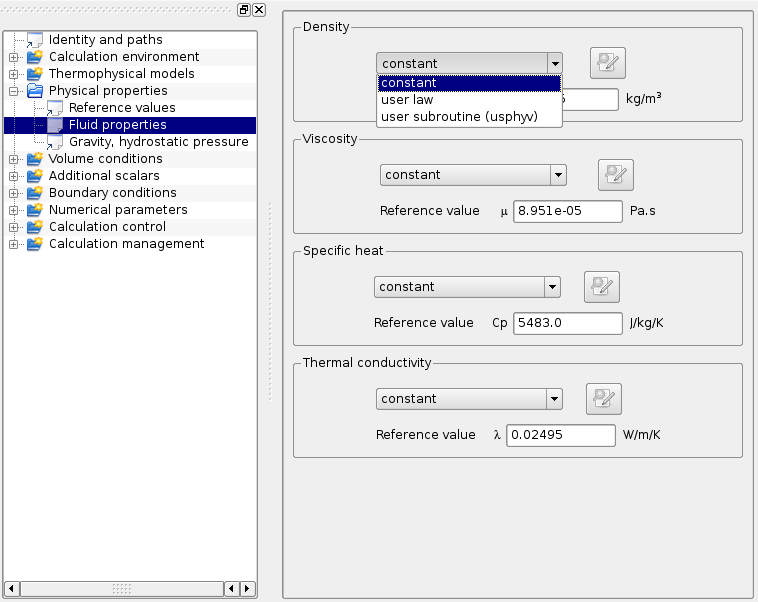
\includegraphics[width=13cm]{gui_fluid_props}
\caption{Physical properties - Fluid properties}
\label{fig:V-60_GUI}
\end{center}
\end{figure}
%
\begin{figure}[!ht]
\begin{center}
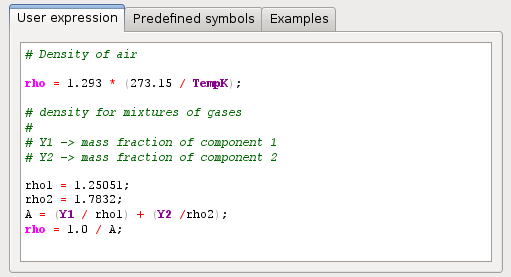
\includegraphics[width=9cm]{gui_density_law}
\caption{Definition of a user law for the density}
\label{fig:UL1_GUI}
\end{center}
\end{figure}

If necessary, all the variation laws related to the fluid physical properties are written in the subroutine \texttt{usphyv}.

The validity of the variation laws must be checked, particularly when
non-linear laws are defined (for instance, a third-degree polynomial law
may produce negative density values).

{\bf \underline{WARNING}}\label{prg_propvar}%
\begin{list}{$\bullet$}{}
\item If one wishes to impose a variable density or variable viscosity in
      \texttt{usphyv}, it must be flagged either in the interface or in
      \texttt{usini1}(\texttt{irovar}=1, \texttt{ivivar}=1).
\item In order to impose a physical property ($\rho$, $\mu$,
      $\lambda$, $C_p$)\footnote{except for some specific physics} a reference
      value should be provided in the interface or in \texttt{usini1} (in
      particular for $\rho$, the pressure will be function of $\rho_0 gz$)
\item By default, the $C_p$ coefficient and the
      diffusivity for the scalars \texttt{iscal} ($\lambda/C_p$ for the
      temperature) are considered as constant in time and uniform in
      space, with the values \texttt{cp0} and \texttt{visls0(iscal)}
      specified in the interface or in \texttt{usini1}.\\
To assign a variable value to $C_p$, the user \textbf{must}t specify it in the
      interface or assign the value 1 to \texttt{icp} in \texttt{usini1},
      and fill for each cell \texttt{iel} the array
      \texttt{propce(iel,ipccp)} in \texttt{usphyv}. Completing the array
      \texttt{propce(iel,ipccp)} while \texttt{icp=0} induces array
      overwriting problems and produces wrong results.

\item In the same way, to have variable diffusivities for the scalars
      \texttt{iscal}, the user \textbf{must} specify it in the interface or give the value
      1 to \texttt{ivisls(iscal)} in \texttt{usini1}, and complete for each cell
      \texttt{iel} the array \texttt{propce(iel,ipcvsl)} in \texttt{usphyv}.
      Completing \texttt{propce(iel,ipcvsl)} while \texttt{ivisls(iscal)}=0
      induces memory overwriting problems and produces wrong results.\\

{\em Example}: If scalars 1 and 3 have a constant and uniform
      diffusivity, and if scalars 2 and 4 have a variable diffusivity,
      the following values must be set in \texttt{usini1}: \\
      \texttt{ivisls(1)}=0, \texttt{ivisls(2)}=1, \texttt{ivisls(3)}=0
      and \texttt{ivisls(4)}=1. \\
      The indicators \texttt{ivisls(2)} and \texttt{ivisls(4)} are then
      modified automatically by the code in order to return the rank
      corresponding to the diffusivity of each scalar in the list of physical
      properties\footnote{they are no longer equal to 1 but stay positive
      so that \texttt{ivisls}$>$0 is synonymous with variable diffusivity}.
      The arrays \mbox{\texttt{propce(iel,ipcvsl)}} in \texttt{usphyv} must
      then be completed with \texttt{ipcvsl=ipproc(ivisls(2))} and
      \texttt{ipcvsl=ipproc(ivisls(4))}. \\

{\em Note}: The indicators \texttt{ivisls} must not be completed in the case of
      user scalars representing the average of the square of the
      fluctuations of another scalar, because the diffusivity of a user
      scalar \texttt{jj} representing the average of the square of the
      fluctuations of a user scalar \texttt{kk} comes directly from the
      diffusivity of this last scalar. In particular, the diffusivity
      of the scalar \texttt{jj} is variable if the diffusivity of \texttt{kk}
      is variable.
\end{list}


%==================================
\subsubsection{Modification of the turbulent viscosity}
%==================================

The subroutine \texttt{usvist} is used to modify the calculation of the turbulent
viscosity, {\em i.e.} $\mu_t$ in $kg.m^{-1}.s^{-1}$
(this piece of information, at the mesh cell centers, is conveyed by the
variable \texttt{propce(iel,ipcvst)}, with
\texttt{ipcvst =  ipproc(ivisct)}). The
subroutine is called at the beginning of every time step, after the
calculation of the physical parameters of the flow and of the
``conventional'' value of $\mu_t$ corresponding to the chosen turbulence
model (indicator \texttt{iturb}).\\
{\em WARNING: The calculation of the turbulent viscosity being a
particularly sensible stage, a wrong use of {\em\texttt{usvist}} may
seriously distort the results.}

%==================================
\subsubsection{Modification of the variable $C$ of the dynamic LES model}
%==================================

\noindent
\textit{Subroutine called every time step in the case of LES with the
dynamic model.}

The subroutine \texttt{ussmag} is used to modify the calculation of the variable $C$ of
the LES sub-grid scale dynamic model.

Let us first remind that the LES approach introduces the notion of
filtering between large eddies and small motions. The solved variables
are said to be filtered in an ``implicit'' way. Sub-grid scale models
(``dynamic'' models) introduce in addition an explicit filtering.

The notations used for the definition of the variable $C$ used in the
dynamic models of \CS are specified below. These notations are the ones
assumed in the document \cite{benhamadouche01}, to which the user may
refer for more details.

The value of $a$ filtered by the explicit filter (of width
$\widetilde{\overline{\Delta}}$) is called $\widetilde{a}$ and the value
of $a$ filtered by the implicit filter (of width $\overline{\Delta}$) is
called $\overline{a}$.
We define:
\begin{equation}
\begin{array}{ll}
\overline{S}_{ij}=\frac{1}{2}(\frac{\partial \overline{u}_i}{\partial x_j}
                  +\frac{\partial \overline{u}_j}{\partial x_i})  &
||\overline{S}||=\sqrt{2 \overline{S}_{ij}\overline{S}_{ij}}\\
\alpha_{ij}=-2\widetilde{\overline{\Delta}}^2
             ||\widetilde{\overline{S}}||
             \widetilde{\overline{S}}_{ij}&
\beta_{ij}=-2\overline{\Delta}^2
             ||\overline{S}||
               \overline{S}_{ij}\\
L_{ij}=\widetilde{\overline{u}_i\overline{u}_j}-
 \widetilde{\overline{u}}_i\widetilde{\overline{u}}_j&
M_{ij}=\alpha_{ij}-\widetilde{\beta}_{ij}\\
\end{array}
\end{equation}


In the framework of LES, the total viscosity (molecular + sub-grid) in
$kg.m^{-1}.s^{-1}$ may be written in \CS:
\begin{equation}
\begin{array}{llll}
\mu_{\text{total}}&=&\mu+\mu_{\text{sub-grid}} &
    \text{\ \ if\ \ }\mu_{\text{sub-grid}}>0\\
                   &=&\mu                          &
    \text{\ \ otherwise }\\
\text{with\ }\mu_{\text{sub-grid}}&=&\rho C \overline{\Delta}^2 ||\overline{S}||
\end{array}
\end{equation}

$\overline{\Delta}$ is the width of the implicit filter, defined at the
cell $\Omega_i$ by \\
$\overline{\Delta}=XLESFL*(ALES*|\Omega_i|)^{BLES}$
\index{xlesfl}\index{ales}\index{bles}.

In the case of the Smagorinsky model (\texttt{iturb=40}), $C$ is a
constant which is worth $C_s^2$. $C_s^2$ is the so-called Smagorinsky
constant and is stored the variable \texttt{$csmago$\index{csmago}}.

In the case of the dynamic model (\texttt{iturb=41}), $C$ is variable in
time and in space. It is determined by
$\displaystyle C=\frac{M_{ij}L{ij}}{M_{kl}M_{kl}}$.

In practice, in order to increase the stability, the code does not use the
value of $C$ obtained in each cell, but an average with the values
obtained in the neighboring cells (this average uses the extended
neighborhood and corresponds to the explicit filter). By default, the
value calculated by the code is
\begin{displaymath}
C=\frac{\widetilde{M_{ij}L{ij}}}{\widetilde{M_{kl}M_{kl}}}
\end{displaymath}

The subroutine \texttt{ussmag} allows to modify this value. It is for
example possible to calculate the local average after having calculated the
ratio
\begin{displaymath}
C=\widetilde{\left[\frac{M_{ij}L{ij}}{M_{kl}M_{kl}}\right]}
\end{displaymath}

{\em WARNING: The subroutine {\em\texttt{ussmag}} can be activated only when
the dynamic model is used.}

%==================================
\subsection{User source terms}
%==================================

Let us assume that the user source terms modify the equation of a
variable $\varphi$ in the following way:
\begin{displaymath}
\rho\frac{\partial \varphi}{\partial t}+\ldots = \ldots + S_{impl}\times\varphi+S_{expl}
\end{displaymath}
The example is valid a velocity component, for a turbulent variable ($k$, $\varepsilon$, $R_{ij}$, $\omega$,
$\varphi$ or $\overline{f}$) and for a scalar (or for the average of the
square of the fluctuations of a scalar), because the syntax of the
subroutines \texttt{ustske}, \texttt{ustsri}, \texttt{ustsv2},
\texttt{ustskw} and \texttt{ustssc} is similar.

In the finite volume formulation, the solved system is then modified as
follows:
\begin{displaymath}
\left(\frac{\rho_i\Omega_i}{\Delta t_i}-\Omega_iS_{impl,i}\right)
\left(\varphi_i^{(n+1)}-\varphi_i^{(n)}\right)
+\ldots = \ldots + \Omega_iS_{impl,i}\varphi_i^{(n)} + \Omega_iS_{expl,i}
\end{displaymath}
The user needs therefore to provide the following values:\\
$\text{\texttt{crvimp}}_i=\Omega_iS_{impl,i}$\\
$\text{\texttt{crvexp}}_i=\Omega_iS_{expl,i}$

In practice, it is essential for the term
$\displaystyle \left(\frac{\rho_i\Omega_i}{\Delta
t_i}-\Omega_iS_{impl,i}\right)$ to be positive. To ensure this property,
the equation really taken into account by the code is the following:
\begin{displaymath}
\left(\frac{\rho_i\Omega_i}{\Delta t_i}-
\text{Min}(\Omega_iS_{impl,i};0)\right)
\left(\varphi_i^{(n+1)}-\varphi_i^{(n)}\right)
+\ldots = \ldots + \Omega_iS_{impl,i}\varphi_i^{(n)} + \Omega_iS_{expl,i}
\end{displaymath}
To make the ``implicitation'' effective, the source term decomposition
between the implicit and explicit parts will be done by the user who must
ensure that $\text{\texttt{crvimp}}_i=\Omega_iS_{impl,i}$ is always negative
(otherwise the solved equation remains right, but there will not be
``implicitation'').

{\em WARNING: When the second-order in time is used along with the extrapolation of the
source terms\footnote{indicator \texttt{isno2t} for the velocity,
\texttt{ISTO2T} for the turbulence and \texttt{isso2t} for the scalars}, it is no longer possible to test the sign of $S_{impl,i}$,
because of coherence reasons (for more details, the user may refer to
the theoretical and computer documentation \cite{theory} of the
subroutine \texttt{preduv}). The user must therefore make sure it is
always positive (or take the risk to affect the calculation stability).}

\minititre{Particular case of a linearised source term}

In some cases, the added source term is not linear, but the user may
want to linearise it using a first-order Taylor development, in order to
make it partially implicit.\\
Let us consider an equation of the type:
\begin{displaymath}
\rho\frac{\partial\varphi}{\partial t}=F(\varphi)
\end{displaymath}
We want to make it implicit using the following method:
\begin{eqnarray*}
\frac{\rho_i\Omega_i}{\Delta t}\left(\varphi_i^{(n+1)}-\varphi_i^{(n)}\right) & = &
\Omega_i\left[F(\varphi_i^{(n)})+\left(\varphi_i^{(n+1)}-\varphi_i^{(n)}\right)
\frac{dF}{d\varphi}(\varphi_i^{(n)})\right]\\
& = & \Omega_i\frac{dF}{d\varphi}(\varphi_i^{(n)})\times\varphi_i^{(n+1)}
+\Omega_i\left[F(\varphi_i^{(n)})-\frac{dF}{d\varphi}(\varphi_i^{(n)})
\times\varphi_i^{(n)}\right]
\end{eqnarray*}

The user must therefore specify:\\
$\displaystyle\text{\texttt{crvimp}}_i=\Omega_i\frac{dF}{d\varphi}(\varphi_i^{(n)})$\\
$\displaystyle\text{\texttt{crvexp}}_i=
\Omega_i\left[F(\varphi_i^{(n)})-\frac{dF}{d\varphi}(\varphi_i^{(n)})\times\varphi_i^{(n)}\right]$

\underline{\em Example}:\\
If the equation is
$\displaystyle \rho\frac{\partial\varphi}{\partial t}=-K\varphi^2$,
the user must set:\\
$\text{\texttt{crvimp}}_i=-2K\Omega_i\varphi_i^{(n)}$\\
$\text{\texttt{crvexp}}_i=K\Omega_i[\varphi_i^{(n)}]^2$

%==================================
\subsubsection{In Navier-Stokes}
%==================================

The subroutine \texttt{ustsns} is used to add user source terms to the Navier-Stokes
equations (at each time step). It is called three times every time
step, once for each velocity component (\texttt{ivar} is successively worth
\texttt{iu}, \texttt{iv} and \texttt{iw}).
At each passage, the user must complete if necessary the arrays \texttt{crvimp}
and \texttt{crvexp} expressing respectively the implicit and explicit part of
the source term. If no other source terms apart from \texttt{ivar=iu} for
example, are required, \texttt{crvimp} and \texttt{crvexp} must be read over and
their 2 other components, \texttt{ivar=iv(ihpas)} and \texttt{ivar=iw}
must be cancelled.

%==================================
\subsubsection{For $k$ and $\varepsilon$}
%==================================

\noindent
\textit{Subroutine called every time step, in $k-\varepsilon$ and
in v2f.}

The subroutine \texttt{ustske} is used to add source terms to the transport equations
related to the turbulent kinetics energy $k$ and to the turbulent
dissipation $\varepsilon$.
This subroutine is called every time step (the
treatment of the two variables $k$ and $\varepsilon$ is made
simultaneously). The user is expected to provide the arrays \texttt{crkimp} and
\texttt{crkexp} for $k$, and \texttt{creimp} and \texttt{creexp} for
$\varepsilon$. These arrays are similar to the arrays \texttt{crvimp} and
\texttt{crvexp} given for the velocity in the user subroutine \texttt{ustsns}.
The way of making implicit the resulting source terms is the same as the one
presented in \texttt{ustsns}. For $\varphi$ and $\bar{f}$
in the v2f model, see \texttt{ustsv2}, \S\ref{prg_ustsv2}.

%==================================
\subsubsection{For $R_{ij}$ and $\varepsilon$}
%==================================

\noindent
\textit{Subroutine called every time step, in $R_{ij}-\varepsilon$.}

The subroutine \texttt{ustsri} is used to add source terms to the transport equations
related to the Reynolds stress variables $R_{ij}$ and to the turbulent
dissipation $\varepsilon$.
This subroutine is called 7 times every time step
(once for each Reynolds stress component and once for the
dissipation). The user must provide the arrays \texttt{crvimp} and
\texttt{crvexp} for the variable \texttt{ivar} (referring successively to
\texttt{ir11}, \texttt{ir22}, \texttt{ir33},
\texttt{ir12}, \texttt{ir13}, \texttt{ir23} and
\texttt{iep}). These arrays are similar to the arrays \texttt{crvimp}
and \texttt{crvexp} given for the velocity in the user subroutine
\texttt{ustsns}. The method for impliciting the resulting source terms is the
same as that presented in \texttt{ustsns}.

%==================================
\subsubsection{For $\varphi$ and $\overline{f}$}
%==================================
\label{prg_ustsv2}

\noindent
\textit{Subroutine called every time step, in v2f.}

The subroutine \texttt{ustsv2} is used to add source terms to the transport equations
related to the variables $\varphi$ and $\overline{f}$ of the v2f
$\varphi$-model. This subroutine is called twice
every time step (once for $\varphi$ and once for $\overline{f}$).
The user is expected to provide the arrays \texttt{crvimp} and
\texttt{crvexp} for \texttt{ivar} referring successively to \texttt{iphi}
and \texttt{ifb}. Concerning $\varphi$, these arrays are similar to the arrays
\texttt{crvimp} and \texttt{crvexp} given for the velocity in the user subroutine
\texttt{ustsns}. Concerning $\overline{f}$, the equation is slightly
different:
\begin{displaymath}
L^2 div(\grad(\overline{f})) = \overline{f} + \ldots + S_{impl}\times\overline{f}+S_{expl}
\end{displaymath}
In the finite volume formulation, the solved system is written as:
\begin{displaymath}
\int_{\partial\Omega_i}\grad(\overline{f})^{(n+1)}dS=\frac{1}{L_i^2}\left(
\Omega_i\overline{f}^{(n+1)}_i + \ldots +  \Omega_iS_{impl,i}\overline{f}_i^{(n+1)} +
\Omega_iS_{expl,i} \right)
\end{displaymath}
The user must then specify:\\
$\text{\texttt{crvimp}}_i=\Omega_iS_{impl,i}$\\
$\text{\texttt{crvexp}}_i=\Omega_iS_{expl,i}$

The way of making implicit the resulting source terms is the same as the
one presented in \texttt{ustsns}.

%==================================
\subsubsection{For $k$ and $\omega$}
%==================================

\noindent
\textit{Subroutine called every time step, in $k-\omega$.}

The subroutine \texttt{ustskw} is used to add source terms to the transport equations
related to the turbulent kinetics energy $k$ and to the specific
dissipation rate $\omega$. This subroutine is
called every time step (the treatment of the two
variables $k$ and $\omega$ is made simultaneously). The user is expected
to provide the arrays \texttt{crkimp} and \texttt{crkexp} for the variable
$k$, and the arrays \texttt{crwimp} and \texttt{crwexp} for the variable $\omega$.
These arrays are similar to the arrays \texttt{crvimp} and \texttt{crvexp}
given for the velocity in the user subroutine \texttt{ustsns}. The way of
making implicit the resulting source terms is the same as the one presented in
\texttt{ustsns}.

%==================================
\subsubsection{For user scalars}
%==================================

\noindent
\textit{Subroutine called every time step.}

The subroutine \texttt{ustssc} is used to add source terms to the transport equations
related to the user scalars (passive or not, average of the square of
the fluctuations of a scalar, ...). In the same way as
\texttt{ustsns}, this subroutine is called every time step, once for
each user scalar. The user needs to provide the arrays \texttt{crvimp}
and \texttt{crvexp} related to each scalar. \texttt{cvimp} and \texttt{crvexp}
must be set to 0 for the scalars on which it is not wished for the user source
term to be applied (the arrays are initially set to 0 at each inlet in the subroutine.)

%==================================
\subsection{Pressure drops (head losses)}
%==================================

Pressure drops can be defined in the Gaphical User Interface (GUI) or in the subroutine \texttt{uskpdc} (called three times every time step). In the GUI, under the heading ``Volume conditions'', the item ``Volume regions definition'' allows to define areas where pressure drops occur, see an example in fig \ref{fig:hl1}. The item ``Head losses'' allows to specify the head loss coefficients, see fig \ref{fig:hl2}. The tensor representing the pressure drops is supposed to be symmetric
and positive.

\begin{figure}[!ht]
\begin{center}
\begin{tabular}{c}
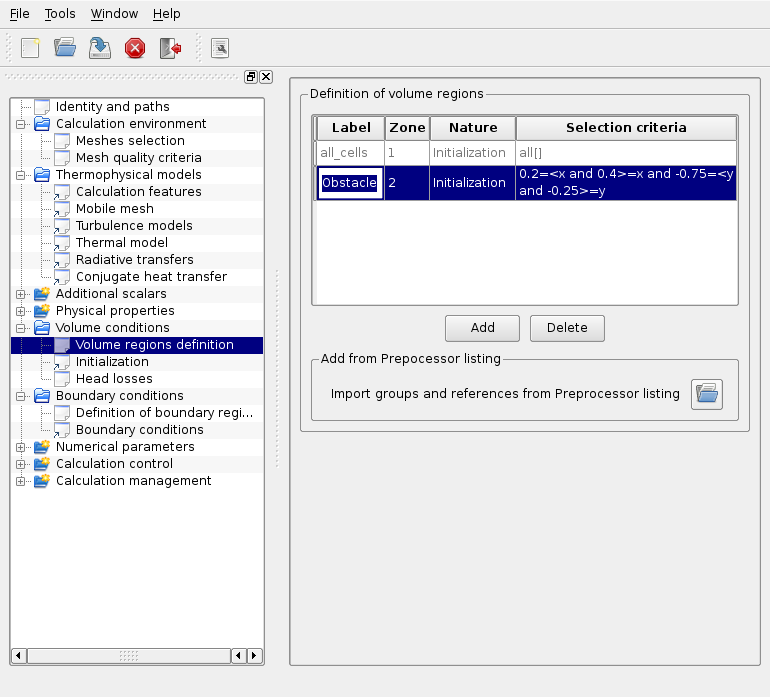
\includegraphics[width=14cm]{gui_volume_regions} \\
\\
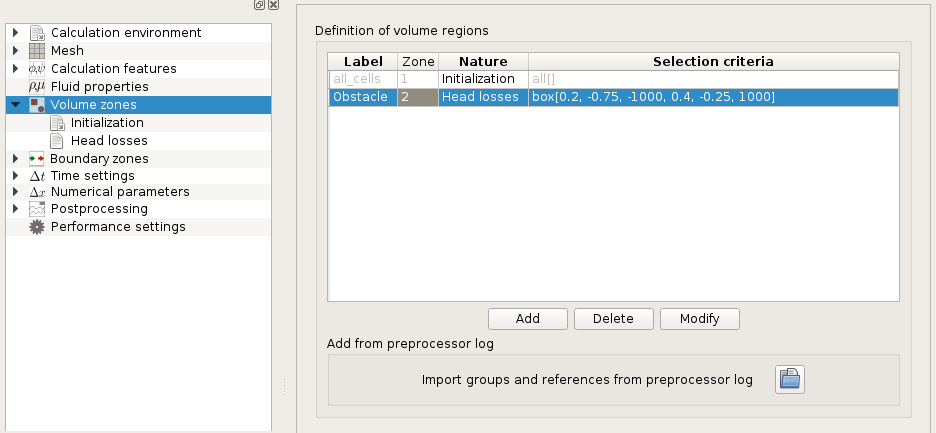
\includegraphics[width=9cm]{gui_head_loss_regions}
\end{tabular}
\caption{Creation of head losses region}
\label{fig:hl1}
\end{center}
\end{figure}
%
\begin{figure}[!ht]
\begin{center}
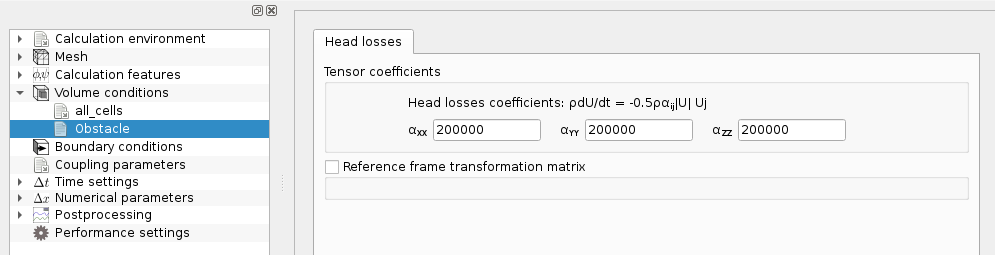
\includegraphics[width=9cm]{gui_head_loss_coeffs}
\caption{Head losses coefficients}
\label{fig:hl2}
\end{center}
\end{figure}

If necessary, the pressure drops are written in the
subroutine \texttt{uskpdc}.

\begin{list}{$\bullet$}{}
\item During the first call, all the cells are checked to know the
      number of cells in which a pressure drop is present.
      This number is called \texttt{ncepdp\index{ncepdp}} in
      \texttt{uskpdc} (and corresponds to
      \texttt{ncepdc\index{ncepdc}}). It is used to lay out the arrays
      related to the pressure drops. If there is no pressure drop,
      \texttt{ncepdp} must be equal to zero (it is the default value, and the
      rest of the subroutine is then useless).

\item During the second call, all the cells are checked again to
      complete the array \texttt{icepdp\index{icepdp}} whose size is
      \texttt{ncepdp}. \mbox{\texttt{icepdc(ielpdc)}} is the number of the
      \texttt{ielpdc}\raisebox{1ex}{\small th} cell containing pressure drops.

\item During the third call, all the cells containing pressure drops
      are checked in order to complete the array
      containing the components of the tensor of pressure drops
      \mbox{\texttt{ckupdc(ncepdp,6)}\index{ckupdc}}. This array is so that
      the equation related to the velocity may be written:
\begin{displaymath}
\rho\frac{\partial}{\partial t}\vect{u}=\ldots -\rho\tens{K}\ind{pdc}\cdot\vect{u}
\end{displaymath}
The tensor components are given in the following order (in the general
      reference frame): \texttt{k11}, \texttt{k22}, \texttt{k33}, \texttt{k12},
      \texttt{k13}, \texttt{k23} with \texttt{k12}, \texttt{k13} and \texttt{k23}
      being zero if the tensor is diagonal.

\end{list}


The three calls are made every time step, so that variable pressure drop
zones or values may be treated.

%==================================
\subsection{Management of the mass sources}
%==================================

The subroutine \texttt{ustsma} is used to add a density source term in some cells of
the domain (called at each time step). The mass conservation equation is then modified as follows:
\begin{displaymath}
\frac{\partial \rho}{\partial t} + div(\rho\vect{u})=\Gamma
\end{displaymath}

$\Gamma$ is the mass source term expressed in $kg.m^{-3}.s^{-1}$.

The presence of a mass source term modifies the evolution equation of
the other variables, too. Let $\varphi$ be a any solved variable apart
from the pressure (velocity component, turbulent energy, dissipation,
scalar, ...). Its evolution equation becomes:
\begin{displaymath}
\rho\frac{\partial \varphi}{\partial t} + \ldots = \ldots + \Gamma(\varphi_i-\varphi)
\end{displaymath}

$\varphi_i$ is the value of $\varphi$ associated with the mass entering
or leaving the domain. After discretisation, the equation may be written:
\begin{displaymath}
\rho\frac{\varphi^{(n+1)}-\varphi^{(n)}}{\Delta t} + \ldots
= \ldots + \Gamma(\varphi_i-\varphi^{(n+1)})
\end{displaymath}

For each variable $\varphi$, there are two possibilities:
\begin{list}{$\bullet$}{}
\item We can consider that the mass is added (or removed) with the
      ambient value of $\varphi$. In this case
      $\varphi_i=\varphi^{(n+1)}$ and the equation of $\varphi$ is not
      modified.
\item Or we can consider that the mass is added with an
      imposed value $\varphi_i$ (this solution is physically correct
      only when the mass is effectively added, $\Gamma>0$).
\end{list}

\bigskip

This subroutine is called three times every time step.

\begin{list}{$\bullet$}{}
\item During the first call, all the cells are checked to know the
      number of cells containing a mass source term.
      This number is called \texttt{ncesmp\index{ncesmp}} in
      \texttt{ustsma} (and corresponds to
      \texttt{ncetsm\index{ncetsm}}). It is used to lay out the arrays
      related to the mass sources. If there is no mass source,
      \texttt{ncesmp} must be equal to zero (it is the default value, and the
      rest of the subroutine is then useless).

\item During the second call, all the cells are checked again to
      complete the array \texttt{icetsm\index{icetsm}} whose dimension is
      \texttt{ncesmp}. \mbox{\texttt{icetsm(ieltsm)}} is the number of the
      \texttt{ieltsm}\raisebox{1ex}{\small th} cell containing a mass source.

\item During the third call, all the cells containing mass sources are
      checked in order to complete the arrays
      \mbox{\texttt{itypsm(ncesmp,nvar)}\index{itypsm}} and
      \mbox{\texttt{smacel(ncesmp,nvar)}\index{smacel}}:\\
- \texttt{itypsm(ieltsm,ivar)} is the flow type associated with the variable
      \texttt{ivar} in the \texttt{ielstm}\raisebox{1ex}{\small th} cell
      containing a mass source.\\
\hspace*{1cm}\texttt{itypsm}=0: $\varphi_i=\varphi^{(n+1)}$ condition\\
\hspace*{1cm}\texttt{itypsm}=1: imposed $\varphi_i$ condition\\
\hspace*{1cm}\texttt{itypsm} is not used for \texttt{ivar=ipr}\\
- \texttt{(ieltsm,ipr)} is the value of the mass source term $\Gamma$, in
$kg.m^{-3}.s^{-1}$.\\
- \texttt{smacel(ieltsm,ivar)}, for \texttt{ivar} different from
\texttt{ipr}, is the value
of $\varphi_i$ for the variable \texttt{ivar} in the
\texttt{ielstm}\raisebox{1ex}{\small th} cell containing a mass source.\\

\minititre{Notes}
$\bullet$ If \texttt{itypsm(ieltsm,ivar)=0}, \texttt{smacel(ieltsm,ivar)}
      is not used.\\
$\bullet$ If $\Gamma$=\texttt{smacel(ieltsm,ipr)}$<$0, mass is removed from
      the system, and \CS considers automatically a
      $\varphi_i=\varphi^{(n+1)}$ condition, whatever the values given
      to \texttt{itypsm(ieltsm,ivar)} and \texttt{smacel(ieltsm,ivar)}
      (the extraction of a variable is done at ambient value).
\end{list}



The three calls are made every time step, so that variable mass source
zones or values may be treated.\\

For the variance, do not take into account the scalar $\varphi_i$ in the environment
where $\varphi\ne\varphi_i$ generates a variance source.

%==================================
\section{Results analysis}
%==================================

%==================================
\subsection{Management of the post-processing intermediate outputs}
%==================================

The subroutine \texttt{usnpst} is used to specify when post-processing outputs will be
generated (it is called at each time step even if the user hasn't moved it to the directory SRC). By default, it tests if the current time step number (\texttt{ntcabs}) is a
multiple of the chosen output frequency (\texttt{ntchr}). If it is the case, the
indicator \texttt{iipost} turns to 1, which triggers the writing of an
intermediate output. If the frequency is given a negative value, the
test is not performed.

For instance, a user who wants to generate post-processing outputs (also
called ``chronological outputs'') at
the time step number 36 and around the physical time $t$=12 seconds may
use the following test:\\

\begin{tabular}{ll}
\mbox{\texttt{iipost = 0}}
                    & No output by default. \\
\mbox{\texttt{if (ntcabs.eq.36) then}}
                    & If the current time step is the 36$^{\text{th}}$,\\
\mbox{\texttt{~~~iipost=1}}
                    & ~~~generate an output. \\
\mbox{\texttt{endif}}
                    & End of the test on the time step number. \\
\mbox{\texttt{if (abs(ttcabs-12.d0).le.0.01d0) then}}
                    & If the physical time is 12s +/- 0.01s,\\
\mbox{\texttt{~~~iipost=1}}
                    & ~~~generate an output. \\
\mbox{\texttt{endif}}
                    & End of the test on the physical time. \\
\end{tabular}

In any case, a post-processing output is generated after the last time
step, \texttt{usnpst} being used or not.

\newpage
%==================================
\subsection{Definition of post-processing and mesh zones}
%==================================

The functions defined in \texttt{cs\_user\_postprocess.c}, namely
\texttt{cs\_user\_postprocess\_writers}, \texttt{cs\_user\_postprocess\_meshes},
and \texttt{cs\_user\_postprocess\_activate} allow for
the definition of postprocessing output formats and frequency, and
for the definition of  surface or volume sections, in the form
of lists of \texttt{nlfac} internal faces (\texttt{lstfac}) and
\texttt{nlfab} boundary faces (\texttt{lstfab}),
or of \texttt{nlcel} cells (\texttt{lstcel}), in order to generate
chronological outputs in {\em EnSight}, {\em MED} or {\em CGNS} format.

One or several writers can be associated with each post-processing
mesh, or ``part'' created. The arguments of the function
\texttt{cs\_post\_define\_writer} are as follows:

\begin{list}{$\bullet$}{}
       \item \texttt{writer\_id}: id the the associated writer.\\
             negative ids are reserved (-1 for the main output),
             but the matching writer's options may be redifined by
             calls to this function.
       \item \texttt{case\_name}: basic name of the associated case.\\ {\em
             WARNING}: depending on the chosen format, this name may
             be shortened (maximum number of characters: 32 for {\em MED},
             19 for {\em EnSight}) or modified automatically (whitespaces or
             forbidden characters will be replaced by '\_')
       \item \texttt{dir\_name}: name of the output directory
       \item \texttt{fmt\_name}: choice of the output format:
        \begin{list}{$\rightarrow$}{}
               \item {\em EnSight Gold} ({\em EnSight} also accepted)
               \item {\em MED}
               \item {\em CGNS}
         \end{list}
The options are not case-sensitive, so {\em ensight} or {\em cgns} are valid, too.
       \item \texttt{fmt\_opts}: character string containing a list of
             options related to the format, separated by commas; for the
             {\em EnSight Gold} format, these options are:
        \begin{list}{$\rightarrow$}{}
               \item {\em binary} for a binary format version (by default)
               \item {\em text} for a text format version
               \item {\em discard\_polygons} to prevent from exporting faces with more
 than four edges (which may not be recognized by some post-processing tools); such
 faces will therefore not appear in the post-processing mesh.
               \item {\em discard\_polyhedra} to prevent from exporting elements which
 are neither tetrahedra, prisms, pyramids nor hexahedra (which may not be recognized by
 some post-processing tools); such elements will therefore not appear in
 the post-processing mesh.
               \item {\em divide\_polygons}  to divide faces with more than four edges
 into triangles, so that any post-processing tool can recognize them
               \item {\em divide\_polyhedra} to divide elements which are neither
 tetrahedra, prisms, pyramids nor hexahedra into simpler elements (tetrahedra and
 pyramids), so that any post-processing tool can recognize them
               \item {\em split\_tensor} to export the components of a tensor
 variable as a series of independent variables (a variable is recognised as a
 tensor if its dimension is 6 or 9); not implemented yet.
         \end{list}
       \item \texttt{time\_dep}: indicates if the post-processing
             (i.e. visualization) meshes (or ``parts'') are:
        \begin{list}{$\rightarrow$}{}
               \item \texttt{FVM\_WRITER\_FIXED\_MESH} fixed (usual case)
               \item \texttt{FVM\_WRITER\_TRANSIENT\_COORDS} deformable
                     (the vertex positions may vary over time)
               \item \texttt{FVM\_WRITER\_TRANSIENT\_CONNECT} modifiable:
                     (the lists of cells or faces
                     defining these meshes can be changed over time)
         \end{list}
       \item \texttt{output\_at\_end}: force output at calculation end
             if not 0
       \item \texttt{frequency\_n}: default output frequency in time steps
             associated with this writer, or $< 0$ (the output may be forced
             or prevented at any time step using the function
             \texttt{cs\_user\_postprocess\_activate})
       \item \texttt{frequency\_t}: default output frequency in seconds
             associated with this writer, or $< 0$ (has priority over
             \texttt{frequency\_n}, and the output may be forced or prevented
             at any time step using the function
             \texttt{cs\_user\_postprocess\_activate})
\end{list}

In order to allow the user to add an output format to
the main output format, or to add a mesh to the default
output, the lists of standard and user meshes and writers are not
separated. Negative numbers are reserved for the non-user items. For
instance,the mesh numbers -1 and -2 correspond respectively to the global
mesh and to boundary faces, generated by default, and the writer -1
corresponds to the usual post-processing case defined {\em via}
\texttt{usini1} or {\em via} the interface.

The user chooses the numbers corresponding to the post-processing
meshes and writers he wants to create. These numbers must be positive
integers. It is possible to assocate a user mesh with the standard
post-processing case (-1), or to ask for outputs regarding the boundary
faces (-2) associated with a user writer.

For safety, the output frequency and the possibility to modify the
post-processing meshes are associated with the writers rather than
with the meshes. This logic avoids unwanted generation of
inconstitent post-processing outputs. For instance EnSight would not
be able to read a case in which one field is output to a given part
every 10 time steps while another field is output to the same part
every 200 time steps.

The possibility to modify a mesh over time is limited by the most restrictive
writer which is associated with. For instance, if writer
1 allows the modification of the mesh topology (argument \texttt{time\_dep
= FVM\_WRITER\_TRANSIENT\_CONNECT} in the call to \texttt{cs\_post\_define\_writer}) and writer 2 allows no
modification (\texttt{time\_dep = FVM\_WRITER\_FIXED\_MESH}),
a user post-processing mesh
associated with the writers 1 and 2 will not be modifiable, but a
mesh associated only with the writer 1 will be modifiable. The
modification may be done by using the advanced
cs\_post\_define\_volume\_mesh\_by\_func() or
cs\_post\_define\_surface\_mesh\_by\_func(), associated with a user-defined
selection function based on time-varying criteria (such as field values
being above a given threshold). If the \texttt{time\_dep} argument is
set to \texttt{true}, the mesh will be redefined using the selection
function at each output time step for every modifiable mesh.

It is possible to output variables which are normally automatically
output on the main volume or boundary meshes to a user mesh which is a subset
of one of these by setting the \texttt{auto\_variables} argument of
one of the \texttt{cs\_post\_define\_...\_mesh} to \texttt{true}.

It is also possible to define an alias of a post-processing mesh. An
alias shares all the attributes of its parent mesh (without duplication),
except its number. This may be used to output different variables on a
same mesh with 2 different writers: the choice of output variables
is based on the mesh, so if $P_a$ is associated with writer $W_a$,
all that is needed is to define an alias $P_b$ to $P_a$ and associate
it with writer $W_b$ to allow a different output variable selection with
each writer. An alias may be created using the \texttt{pstalm} subroutine.

Modification of a postprocessing mesh or it's alias over time is always
limited by the most restrictive "writer" to which it's meshes have been
asscoiated (parts of the structures being shared in memory). It is
possible to define as many aliases as are required for a true mesh,
but an alias cannot be defined for another alias.

It is not possible to mix cells and faces in the same mesh (most of
the post-processing tools being perturbed by such a case)\footnote{actually,
faces adjacent to selected cells and belonging to face or cell groups
may be selected when the \texttt{add\_groups} of
\texttt{cs\_post\_define\_...\_mesh} is set to \texttt{true},
so as to maintain group information, but those faces will
only be written for formats supporting this (such as MED),
and will only bear groups, not variable fields}.

For a better understanding, the user may refer to the examples given in
\texttt{cs\_user\_postprocess\_meshes}. We can note that the whitespaces
in the beginning or in the end of the character strings given as arguments
of the functions called are suppressed automatically.

The additional variables to post-process on the defined meshes
will be specified in the subroutine \texttt{usvpst}.  ``

{\em WARNING In the parallel case, some meshes may not contain any
local elements on a given processor. This is not a problem at all, as
long as the mesh is defined for all processors (empty or not).
It would in fact not be a good idea at all to define a postprocessing
mesh only if it contains local elements, global operations on that
mesh would become impossible, leading to probable deadlocks or crashes.}

%==================================
\subsection{Definition of the variables to post-process}
%==================================

For the mesh parts defined using the GUI or in \texttt{cs\_user\_postprocess.c},
the \texttt{usvpst} subroutine  may be used to specify the variables to
post-process (called for each ``part'', at every active time step of an
associated ``writer'', see \texttt{cs\_user\_postprocess.c}.

The output of a given variable is generated by means of a call to
\texttt{psteva}, whose arguments are:

\begin{list}{$\bullet$}{}
       \item \texttt{nummai}: current ``part'' number (input
             argument in \texttt{usvpst}).
       \item \texttt{namevr}: name to give to the variable.
       \item \texttt{idimt}: dimension of the variable (3 for a vector, 1 for
             a scalar).
       \item \texttt{ientla}: indicates if the stored arrays are
             ``interlaced'' or not:
        \begin{list}{$\rightarrow$}{}
               \item 0: not interlaced, in the form ${\{x_1, x_2, ..., x_n,
                         y_1, y_2, ..., y_n, z_1, z_2, ..., z_n\}}$ \\
                         (case of all variables defined in \texttt{rtp}).
               \item 1: interlaced, in the form ${\{x_1, y_1, z_1, x_2, y_2, z_2, ..., x_n, y_n, z_n\}}$ \\
                         (case of the geometric parameters, like
                     \texttt{xyzcen}, \texttt{surfbo}, ...).
         \end{list}
              For a scalar variable, this argument does not matter.
       \item \texttt{ivarpr}: indicates if the variable is defined on the
             ``parent'' mesh or locally:
        \begin{list}{$\rightarrow$}{}
               \item 0: variable generated by the user in the given work
                     arrays \texttt{tracel}, \texttt{trafac}, and
                     \texttt{trafbr} (whose size is respectively the
                     number of cells, internal faces and boundary faces
                     of the ``part'', $\times 3$). The arrays
                     \texttt{lstcel}, \texttt{lstfac}, and
                     \texttt{lstfbr} can be used to get the numbers
                     corresponding to the cells, internal faces and
                     boundary faces associated with the ``part'' and to
                     generate the appropriate post-processing variable.
               \item 1: variable already defined in the main mesh
                     (``parent'' mesh of the ``parts''), for example the
 variables in the rtp array. Instructions in the report which list\texttt
{lstcel}, \texttt{lstfac}, and \texttt{lstfbr}will be treated directly by
 the sub routine, avoiding unused copies and simplifying hte code
         \end{list}
       \item \texttt{ntcabs}: absolute current time step number. If a
             negative value is given (usually -1), the variable will be
             regarded  as time-independent (and we will have to make sure this
             call is only made once).
       \item \texttt{ttcabs}: current physical time value. It is not taken
             into account if \texttt{ntcabs} $< 0$.
       \item \texttt{tracel}: array containing the values of the
             variable at the cells. If \texttt{ivarpr} $= 1$, this
             argument will be replaced by the position of the beginning
             of the array on which the variable in defined, for instance
             \texttt{rtp(1, iu(1))} for the velocity.
       \item \texttt{trafac}: equivalent of \texttt{tracel} for the
             internal faces.
       \item \texttt{trafbr}: equivalent of \texttt{tracel} for the
             boundary faces.
\end{list}

The user may refer to the example, which presents the different ways of
generating an output of a variable.

{\em WARNING: Apart from the time-independent variables, it is not
recommended not to generate the same variables at every call
(corresponding to an active time step) for a given mesh, because the
post-processing tool may have difficulties to deal with such a case. To
generate outputs of different variables on the same mesh with different
frequencies, it is recommended to create an alias of this mesh and to
associate it with a different ``writer'' using the GUI or in
\texttt{cs\_user\_postprocess.c}.}

%==================================
\subsection{Modification of the variables at the end of a time step}
%==================================

The subroutine \texttt{usproj} is called at the end of every time step. It is used to
print of modify any variable at the end of every time step.

Several examples are given:
\begin{list}{-}{}
\item Calculation of a thermal balance at  the boundaries and in the
      domain (including the mass source terms)

\item Modification of the temperature in a given area starting from a
      given time

\item Extraction of a 1D profile, see fig. \ref{fig:26_GUI}

\item Printing of a moment

\item Utilisation of utility
      subroutines useful in the case of a parallel calculation
      (calculation of a sum on the processors, of a maximum, ...)
\end{list}

{\em WARNING: As all the variables (solved variables, physical
properties, geometric parameters) can be modified in this subroutine, a
wrong use may distort totally the calculation.}

The thermal balance example is particularly interesting.
\begin{list}{-}{}
\item It can be easily adapted to another scalar (only three simple
      modifications to do, as indicated in the subroutine).
\item It shows how to make a sum on all the subdomains in the framework
      of a parallel calculation (see the calls to the subroutines
      \texttt{par*}).
\item It shows the precautions to take before doing some operations in
      the framework of periodic or parallel calculations (in particular
      when we want to calculate the gradient of a variable or to have
      access to values at the cells neighboring a face).
\item Finally it must not be forgotten that the resolution with
      temperature as a solved variable is questionable when the specific
      heat is not constant.
\end{list}

%==================================
\subsection{Non-standard management of the chronological record files}
%==================================
\label{prg_ushist}

The interface and the subroutine \texttt{usini1} allow to manage the
``automatic'' chronological record files in an autonomous way:
position of the probes, printing frequency and related variables. The
results are written in a different file for each variable. These files
are written in {\em xmgrace or {\em gnuplot}} format and contain the profiles corresponding to
every probe. This type of output format may not be well adapted if, for
instance, the number of probes is too high. The subroutine
\texttt{ushist}, called at each time step, allows then to personalise the output format of the
chronological record files. The version given as example in the
directory works as follows:

\begin{list}{-}{}
\item Positionning of the probes (only at the first passage): the index
      \texttt{ii} varies between 1 and the number of probes. The coordinates
      \texttt{xx}, \texttt{yy} and \texttt{zz} of each probe are given.
      The subroutine \texttt{findpt}
      gives then the number \texttt{icapt(ii)\index{icapt}} of the cell center
      which is the closest to the defined probe.

\item Opening of the output files (only at the first pass): in the
      version given as example, the program opens a different file for
      all the \texttt{nvar} variables. \texttt{ficush(j)} contains the name of the
      J\raisebox{1ex}{\small th} file and \texttt{impush(j)} its unit number
      (\texttt{impush} is initialised by default so that the user has at his
      disposal specific unit numbers and does not run the risk to overwrite an
      already open file).

\item Writing to the files: in the version given as example, the program
      writes the time step number, the physical time step (based on the
      standard time step in the case of a variable time step) and the
      value of the selected variable at the different probes.

\item Closing of the files (only at the last time step).

\end{list}

{\em WARNING: The use of {\em\texttt{ushist}} neither erases nor replaces the
parameters given in the interface or in {\em\texttt{usini1}}. Therefore, in
the case of the use of {\em\texttt{ushist}}, and to avoid the creation
of useless files, the user should set {\em \texttt{ncapt}=0} in the interface or
in {\em \texttt{usini1}} to deactivate the automatic production of
chronological records}.\\
In addition, {\em \texttt{ushist}} generates supplementary result
files.


%==================================
\section{Advanced modelling setup}
%==================================

%==================================
\subsection{Use of a specific physics}
%==================================
\label{prg_usppmo}%
Specific physics such as dispersed phase, atmospheric flows and coal combustion models can be added by the user from the interface, or by using the subroutine \texttt{usppmo} (called only during the calculation initialisation). With the interface, when a specific physics is activated in fig. \ref{fig:5_GUI}, additional items or headings may appear (see for instance Sections \ref{sec:Ini-lag} and \ref{sec:Ini-coal}).

\begin{figure}[!ht]
\begin{center}
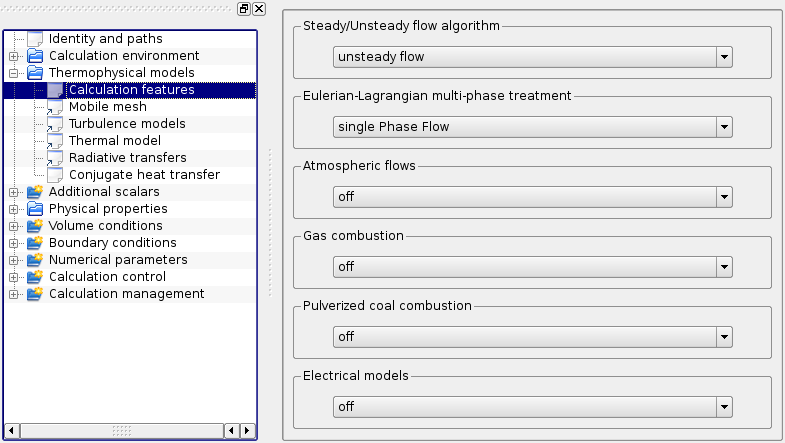
\includegraphics[width=14cm]{gui_thermo_phys_models}
\caption{Thermophysical models selection}
\label{fig:5_GUI}
\end{center}
\end{figure}

When the interface is not used, \texttt{usppmo} is one of the three subroutines which must be obligatory completed by the user in order to use a specific physics module. Also, some specific physics modules can not yet be activated through the interface such as the modules listed below which were not quoted at the beginning of this section.
At the moment, \CS allows to use two ``pulverised coal'' modules
(with Lagrangian coupling or not), two ``gas combustion'' modules, two
``electrical'' modules, a ``compressible'' module, an ``cooling towers'' module and an ``atmospheric'' module. To activate one of
these modules, the user needs to complete one (and only one) of the
indicators \texttt{ippmod(i.....)\index{ippmod}} in the subroutine
\texttt{usppmo}. By default, all the indicators \texttt{ippmod(i.....)} are
initialised at -1, which means that no specific physics is activated.

\begin{list}{$\bullet$}{}
       \item Diffusion flame in the framework of ``3 points'' rapid complete
             chemistry: indicator {\bf \tt ippmod(icod3p\index{icod3p})}
        \begin{list}{$\rightarrow$}{}
               \item \texttt{ippmod(icod3p)} = 0 adiabatic conditions
               \item \texttt{ippmod(icod3p)} = 1 permeatic conditions (enthalpy
                     transport)
               \item \texttt{ippmod(icod3p)} =-1 module not activated
         \end{list}
        \item Eddy Break Up pre-mixed flame: indicator {\bf \tt
             ippmod(icoebu\index{icoebu})}
         \begin{list}{$\rightarrow$}{}
                \item \texttt{ippmod(icoebu\index{icoebu})} = 0 adiabatic
                      conditions at constant richness
                \item \texttt{ippmod(icoebu)} = 1 permeatic conditions at
                      constant richness
                \item \texttt{ippmod(icoebu)} = 2 adiabatic conditions at
                      variable richness
                \item \texttt{ippmod(icoebu)} = 3 permeatic conditions at
                      variable richness
                \item \texttt{ippmod(icoebu)} =-1 module not activated
         \end{list}
        \item Libby-Williams pre-mixed flame: indicator {\bf \tt ippmod(icolwc\index{icolwc})}
         \begin{list}{$\rightarrow$}{}
               \item \texttt{ippmod(icolwc)}=0 two peak model with adiabiatic conditions.
               \item \texttt{ippmod(icolwc)}=1 two peak model with permeatic conditions.
               \item \texttt{ippmod(icolwc)}=2 three peak model with adiabiatic conditions.
               \item \texttt{ippmod(icolwc)}=3 three peak model with permeatic conditions.
               \item \texttt{ippmod(icolwc)}=4 four peak model with adiabiatic conditions.
               \item \texttt{ippmod(icolwc)}=5 four peak model with permeatic conditions.
               \item \texttt{ippmod(icolwc)}=-1 module not activated.
          \end{list}
        \item Multi-coals and multi-classes pulverised coal combustion:
              indicator {\bf \tt ippmod(icp3pl\index{icp3pl})}
              The number of different coals must be inferior or equal to
              \texttt{ncharm\index{ncharm}} = 3. The number of particle size
             classes \texttt{nclpch\index{nclpch}(icha)} for the coal
             \texttt{icha}, must
             be inferior or equal to \texttt{ncpcmx\index{ncpcmx}} = 10.
         \begin{list}{$\rightarrow$}{}
                \item \texttt{ippmod(icp3pl)} = 0 imbalance between the
                      temperature of the continuous and the solid phases
                \item \texttt{ippmod(icp3pl)} = 1 otherwise
                \item \texttt{ippmod(icp3pl)} =-1 module not activated
         \end{list}
        \item Lagrangian modeling of multi-coals and
             multi-classes pulverised coal combustion:
                 indicator {\bf \tt ippmod(icpl3c\index{icpl3c})}
              The number of different coals must be inferior or equal to
              \texttt{ncharm\index{ncharm}} = 3. The number of particle size
             classes \texttt{nclpch\index{nclpch}(icha)} for the coal
             \texttt{icha}, must be inferior or equal to
             \texttt{ncpcmx\index{ncpcmx}} = 10.
         \begin{list}{$\rightarrow$}{}
                \item \texttt{ippmod(icpl3c)} = 1 coupling with the Lagrangian
                      module, with transport of $H_2$
                \item \texttt{ippmod(icpl3c)} =-1 module not activated
         \end{list}
       \item Electric arc module (Joule effect and Laplace forces):
             indicator {\bf \tt ippmod(ielarc\index{ielarc})}
        \begin{list}{$\rightarrow$}{}
               \item \texttt{ippmod(ielarc)} = 1 determination of the magnetic field by
                     means of the Ampere's theorem (not available)
               \item \texttt{ippmod(ielarc)} = 2 determination of the magnetic
                     field by means of the vector potential
               \item \texttt{ippmod(ielarc)} =-1 module not activated
         \end{list}
       \item Joule effect module (Laplace forces not taken into account):
             indicator {\bf \tt ippmod(ieljou\index{ieljou})}
        \begin{list}{$\rightarrow$}{}
               \item \texttt{ippmod(ieljou)} = 1 use of a real potential
               \item \texttt{ippmod(ieljou)} = 2 use of a complex potential
               \item \texttt{ippmod(ieljou)} = 3 use of real potential and specific boundary conditions for transformers.
               \item \texttt{ippmod(ieljou)} = 4 use of complex potential and specific boundary conditions for transformers.
               \item \texttt{ippmod(ieljou)} =-1 module not activated
         \end{list}
       \item Compressible module: indicator {\bf \tt
             ippmod(icompf\index{icompf})}
        \begin{list}{$\rightarrow$}{}
               \item \texttt{ippmod(icompf)} = 0 module activated
               \item \texttt{ippmod(icompf)} =-1 module not activated
         \end{list}
       \item atmospheric flow module: indicator {\bf \tt
             ippmod(iatmos\index{icompf})}
        \begin{list}{$\rightarrow$}{}
               \item \texttt{ippmod(iatmos)} =-1 module not activated
               \item \texttt{ippmod(iatmos)} = 0 standard modelling
               \item \texttt{ippmod(iatmos)} = 1 dry atmosphere
               \item \texttt{ippmod(iatmos)} = 2 humid atmosphere (NOT functional)
         \end{list}
       \item cooling towers module: indicator {\bf \tt
             ippmod(iaeros\index{icompf})}
        \begin{list}{$\rightarrow$}{}
               \item \texttt{ippmod(iaeros\index)} =-1 module not activated
               \item \texttt{ippmod(iaeros\index)} = 0 no model (NOT functional)
               \item \texttt{ippmod(iaeros\index)} = 1 Poppe's model
               \item \texttt{ippmod(iaeros\index)} = 2 Merkel's model
         \end{list}
\end{list}

{\em WARNING: Only one specific physics module can be activated at the
same time.}

In the framework of the gas combustion modeling, the user may impose
his own enthalpy-temperature tabulation (conversion law). He needs then
to give the
value zero to the indicator \texttt{indjon\index{indjon}} (the default value
being 1). For more details, the user may refer to the following note
(thermo-chemical files).

\minititre{Note: the thermo-chemical files}
The user must not forget to place in the directory DATA the
thermo-chemical file \texttt{dp\_FCP}, \texttt{dp\_C3P}, \texttt{dp\_C3PSJ} or
\texttt{dp\_ELE} (depending on the specific physics module he activated)
and to specify the name of this file in the variable
THERMOCHEMISTRY\_DATA in the launch script
(for instance: THERMOCHEMISTRY\_DATA''dp\_C3P''). Some example files
are placed in the directory \texttt{DATA/THCH} at the creation of the
study case. Their content is described below.

\begin{list}{$\bullet$}{}
       \item Example of file for the gas combustion:
        \begin{list}{$\rightarrow$}{}
               \item if the enthalpy-temperature conversion data base
                     JANAF is used: \texttt{dp\_C3P} (see
                     array\ref{tab_dpC3P}).

\begin{table}[htbp]
\begin{center}
\small{
\begin{tabular}{|c|c|c|c|} \hline
 Lines  &Examples of values &        Variables             & Observations                                     \\ \hline
  1     &         5         &  \texttt{ngaze\index{ngaze}} & Number of current species                        \\ \hline
  2     &        10         &   \texttt{npo\index{npo}}    & Number of points for the                         \\
        &                   &                              & enthalpy-temperature tabulation                  \\ \hline
  3     &       300.        &  \texttt{tmin\index{tmin}}   & Temperature inferior limit                       \\
        &                   &                              & for the tabulation                               \\ \hline
  4     &      3000.        &  \texttt{tmax\index{tmax}}   & Temperature superior limit                       \\
        &                   &                              & for the tabulation                               \\ \hline
  5     &                   &                              & Empty line                                       \\ \hline
  6     & CH4 O2 CO2 H2O N2 &  \texttt{nomcoe\index{nomcoe}}(\texttt{ngaze}) & List of the current species                      \\ \hline
  7     &.35 .35 .35 .35 .35&  \texttt{kabse\index{kabse}}(\texttt{ngaze})   & Absorption coefficient                           \\
        &                   &                              & of  the current species                          \\ \hline
  8     &         4         &  \texttt{nato\index{nato}}   & Number of elemental species                      \\ \hline
  9     &.012  1  0  1  0  0& \texttt{wmolat\index{wmolat}}(\texttt{nato}),  & Molar mass of the elemental                      \\
 10     &.001  4  0  0  2  0&                              & species (first column)                           \\
 11     &.016  0  2  2  1  0&\texttt{atgaze\index{atgaze}}(\texttt{ngaze},\texttt{nato})& Composition of the current species             \\
 12     &.014  0  0  0  0  2&                              & as a function of the elemental species           \\
        &                   &                              & (\texttt{ngaze} following columns)                        \\ \hline
 13     &         3         &  \texttt{ngazg\index{ngazg}} & Number of global species                         \\
        &                   &                              & Here, \texttt{ngazg} = 3 (Fuel, Oxidiser and Products)    \\ \hline
 14     &  1. 0. 0. 0. 0.   &                              & Composition of the global species as a           \\
 15     &  0. 1. 0. 0. 3.76 &\texttt{compog\index{compog}}(\texttt{ngaze},\texttt{ngazg})& fonction of the current species of the line 6 \\
 16     &  0. 0. 1. 2. 7.52 &                              & In the order: Fuel (line 15),                    \\
        &                   &                              & Oxidiser (line 16) and Product (line 17)         \\ \hline
 17     &         1         &  \texttt{nrgaz\index{nrgaz}} & Number of global reactions                       \\
        &                   &                              & Here \texttt{nrgaz} = 1 (always equal to 1                \\
        &                   &                              & in this version)                                 \\ \hline
 18     &                   & \texttt{igfuel\index{igfuel}}(\texttt{nrgaz}), & Numbers of the global species concerned by       \\
        & 1 2 -1 -9.52 10.52&  \texttt{igoxy\index{igoxy}}(\texttt{nrgaz}),  & the stoichiometric ratio                         \\
        &                   &                              & (first 2 integers)                               \\
        &                   &\texttt{stoeg\index{stoeg}}(\texttt{ngazg},\texttt{nrgaz})& Stoichiometry in reaction global species.       \\
        &                   &                               & Negative for the reactants (here                \\
        &                   &                               & ``Fuel'' and ``Oxidiser'') and positive for      \\
        &                   &                               & the products (here ``Products'')                \\ \hline
\end{tabular}
}
\caption{Example of file for the gas combustion when JANAF is used: \texttt{dp\_C3P}}\label{tab_dpC3P}
\end{center}
\end{table}

               \item if the user provides his own enthalpy-temperature tabulation
                     (there must be three chemical species and only
                     one reaction): \texttt{dp\_C3PSJ} (see
                     array \ref{tab_dpC3PSJ}). This file replaces \texttt{dp\_C3P}.

\begin{table}[htbp]
\begin{center}
\small{
\begin{tabular}{|c|c|c|c|} \hline
 Lines  &            Examples of values     &        Variables            & Observations                                \\ \hline
   1    &                    6              &   \texttt{npo}              & Number of tabulation points                 \\ \hline
   2    &  50. -0.32E+07 -0.22E+06 -0.13E+08&                             &                                             \\
   3    & 250. -0.68E+06 -0.44E+05 -0.13E+08&\texttt{th\index{th}}(\texttt{npo}),           & Temperature(first column),                  \\
   4    & 450.  0.21E+07  0.14E+06 -0.13E+08& \texttt{ehgazg\index{ehgazg}}(1,\texttt{npo}),& mass enthalpy of fuel, oxidiser             \\
   5    & 650.  0.50E+07  0.33E+06 -0.12E+08& \texttt{ehgazg}(2,\texttt{npo}),              & and products (columns 2,3 and 4)            \\
   6    & 850.  0.80E+07  0.54E+06 -0.12E+08& \texttt{ehgazg}(3,\texttt{npo})               & from line 2 to line \texttt{npo}+1                   \\
   7    &1050.  0.11E+08  0.76E+06 -0.11E+08&                             &                                             \\ \hline
   8    & .00219       .1387        .159    &\texttt{wmolg(1)\index{wmolg}},       & Molar mass of fuel,                         \\
        &                                   &                    \texttt{wmolg(2)},& oxidiser                                    \\
        &                                   &                    \texttt{wmolg(3)} & and products                                \\ \hline
   9    &                .11111             &          \texttt{fs(1)\index{fs(1)}} & Mixing rate at the stoichiometry            \\
        &                                   &                             & (relating to Fuel and Oxidiser)             \\ \hline
  10    &    0.4      0.5       0.87        &\texttt{ckabsg\index{ckabsg}(1)},     & Absorption coefficient of fuel,             \\
        &                                   &                  \texttt{ckabsg(2)}, & oxidiser                                    \\
        &                                   &                  \texttt{ckabsg(3)}  & and products                                \\ \hline
  11    &    1.       2.                    & \texttt{xco2\index{xco2}},   \texttt{xh2o\index{xh2o}}& Molar coefficents of $CO_2$         \\
        &                                   &                             & and $H_2O$ in the products                  \\
        &                                   &                             & (radiation using Modak)                     \\ \hline
\end{tabular}
}
\caption{Example of file for the gas combustion when the user provides
 his own enthalpy-temperature tabulation
                     (there must be three species and only one
                     reaction): \texttt{dp\_C3PSJ} (this file replaces
 \texttt{dp\_C3P})}\label{tab_dpC3PSJ}
\end{center}
\end{table}
        \end{list}

       \item Example of file for the pulverised coal combustion:
             \texttt{dp\_FCP} (see array \ref{tab_dpFCP}).

\begin{table}[htbp]
\begin{center}
\tiny{
\begin{tabular}{|c|c|c|c|} \hline
 Lines  &      Examples of values        &        Variables              & Observations                                         \\ \hline
   1    &          THERMOCHEMISTRY       &                               & Comment line                                         \\ \hline
   2    &               8                & \texttt{ncoel\index{ncoel}}   & Number of current species                            \\ \hline
   3    &               8                &  \texttt{npo\index{npo}}      & Number of points for the                             \\
        &                                &                               & enthalpy-temperature tabulation                      \\ \hline
   4    &        CURRENT SPECIES         &                               & Comment line                                         \\ \hline
   5    & CH4 C2H4 CO O2 CO2 H2O N2 C(S) & \texttt{nomcoel\index{nomcoel}}(\texttt{ncoel}) & List of the                                          \\
        &                                &                               & current species                                      \\ \hline
   6    &               300.             &  \texttt{tmin\index{tmin}}    & Temperature inferior limit (Kelvin)                  \\
        &                                &                               & for the enthalpy-temperature tabulation              \\ \hline
   7    &              2400.             &  \texttt{tmax\index{tmax}}    & Temperature superior limit (Kelvin)                  \\
        &                                &                               & for the enthalpy-temperature tabulation              \\ \hline
   8    &               4                &  \texttt{nato\index{nato}}    & Number of elementary species                          \\ \hline
   9    &  .012  1  2  1  0  1  0  0  1  &                               & Molar mass of the elemental species                  \\
  10    &  .001  4  4  0  0  0  2  0  0  &\texttt{wmolat\index{wmolat}}(\texttt{nato}),    & (first column)                                       \\
  11    &  .016  0  0  1  2  2  1  0  0  &\texttt{atcoel\index{atcoel}}(\texttt{ncoel,nato})& and composition of the current species              \\
  12    &  .014  0  0  0  0  0  0  2  0  &                               & as a function of the elemental species               \\ \hline
  13    &          RADIATION             &                               & Comment line                                         \\ \hline
  14    &               0.1              & \texttt{ckabs1\index{ckabs1}}  & Constant absorption coefficient                      \\
        &                                &                               & for the gas mixture                                  \\ \hline
  15    &   COAL CHARACTERISTICS         &                               & Comment line                                         \\ \hline
  16    &               2                & \texttt{ncharb\index{ncharb}} & Number of coal types                                 \\ \hline
  17    &         1            1         & \texttt{nclpch\index{nclpch}}(\texttt{ncharb}) & Number of classes for each coal                      \\
        &                                &                               & (each column corresponding to                        \\
        &                                &                               & one coal type )                                      \\ \hline
  18    &    50.E-6        50.E-6        & \texttt{diam20\index{diam20}}(\texttt{nclacp})  & Initial diameter of each class (m)                   \\
        &                                &                               & \texttt{nclacp\index{nclacp}} is the total number of classes. \\
        &                                &                               & All the diameters are written on the same line       \\
        &                                &                               & (sucessively for each coal, we give the              \\
        &                                &                               & diameter corresponding to each class)                \\ \hline
  19    &    74.8          60.5          & \texttt{cch\index{cch}}(\texttt{ncharb})& Composition in C (mass.-\%, dry) of each coal        \\ \hline
  20    &     5.1           4.14         & \texttt{hch\index{hch}}(\texttt{ncharb})& Composition in H (mass.-\%, dry) of each coal        \\ \hline
  21    &    12.01          5.55         & \texttt{och\index{och}}(\texttt{ncharb})& Composition in O (mass.-\%, dry) of each coal        \\ \hline
  22    & 0  31524000.    0  31524000.   & \texttt{ipci\index{ipci}}(\texttt{ncharb})      & Value of the PCI ($Jkg^{-1}$) for each coal,         \\
        &                                & \texttt{pcich\index{pcich}}(\texttt{ncharb})    & the first integer indicating if this value refers    \\
        &                                &                               & to pure (0) or dry coal (1)                          \\ \hline
  23    &   1800.      1800.             & \texttt{cp2ch\index{cp2ch}}(\texttt{ncharb})& Heat-storage capacity at constant pressure        \\
        &                                &                               & ($Jkg^{-1}K^{-1}$) for each coal                     \\ \hline
  24    &   1200.      1200.             & \texttt{rho0ch\index{rho0ch}}(\texttt{ncharb})   & Initial density ($kgm^{-3}$) of each                 \\ \hline
  25    &          Coke                  &                               & Comment line                                         \\ \hline
  26    &      0.         0.             & \texttt{cck\index{cck}}(\texttt{ncharb}) & Composition in C (mass.-\%, dry) of the coke         \\
        &                                &                               & for each coal                                        \\ \hline
  27    &      0.         0.             & \texttt{hck\index{hck}}(\texttt{ncharb}) & Composition in H (mass.-\%, dry) of the coke         \\
        &                                &                               & for each coal                                        \\ \hline
  28    &      0.         0.             & \texttt{ock\index{ock}}(\texttt{ncharb}) & Composition in O (mass.\%, dry) of the coke          \\
        &                                &                               & for each coal                                        \\ \hline
  29    &      0.         0.             & \texttt{pcick\index{pcick}}(\texttt{ncharb})& PCI of the dry coke ($Jkg^{-1}$) for each coal       \\ \hline
  30    &          Ashes               &                               & Comment line                                         \\ \hline
  31    &      6.3        6.3            & \texttt{xashch\index{xashch}}(\texttt{ncharb})& Ash mass fraction (mass.-\%, dry) in each coal       \\ \hline
  32    &      0.         0.             & \texttt{h0ashc\index{h0ashc}}(\texttt{ncharb})  & Ash formation enthalpy ($Jkg^{-1}$)                  \\
        &                                &                               & for each coal                                        \\ \hline
  33    &      0.         0.             & \texttt{cpashc\index{cpashc}}(\texttt{ncharb})   & CP of the ashes ($Jkg^{-1}K^{-1}$) for each coal     \\ \hline
  34    &      0.         0.             & \texttt{xwatch\index{cpashc}}(\texttt{ncharb})   & humidity rate of the ashes (mass.-\%) for each coal     \\ \hline
  35    &  Devolatilisation (Kobayashi)  &                             & Comment line                                         \\ \hline
  36    &  1  0.37      0  0.37          & \texttt{iy1ch\index{iy1ch}}(\texttt{ncharb}),   & For each coal, pairs (\texttt{iy1ch}, \texttt{y1ch}).                  \\
        &                                & \texttt{y1ch\index{y1ch}}(\texttt{ncharb})     & The real \texttt{y1ch} is the adimensional stoich. coefficient\\
        &                                &                               & If the integer \texttt{iy1ch} is worth 1,                     \\
        &                                &                               & the provided value of \texttt{y1ch} is adopted and            \\
        &                                &                               & the composition of the light volatile matters        \\
        &                                &                               & is calculated automatically.                         \\
        &                                &                               & If the integer \texttt{iy1ch} is worth 0,                     \\
        &                                &                               & the provided value of \texttt{y1ch} is ignored:               \\
        &                                &                               & \texttt{y1ch} is calculated automatically (the light          \\
        &                                &                               & volatiles are then composed of {$CH_{4}$}, {$CO$}).  \\ \hline
  37    &  1  0.74      1  0.74          & \texttt{iy2ch\index{iy2ch}}(\texttt{ncharb}),   & For each coal, pairs (\texttt{iy2ch}, \texttt{y2ch}).                  \\
        &                                & \texttt{y2ch\index{y2ch}}(\texttt{ncharb})     & The real \texttt{y2ch} is the adimensional stoich. coefficient\\
        &                                &                               & If the integer \texttt{iy2ch} is worth 1,                     \\
        &                                &                               & the provided value of \texttt{y2ch} is adopted and            \\
        &                                &                               & the composition of the heavy volatile matters        \\
        &                                &                               & is calculated automatically.                         \\
        &                                &                               & If the integer \texttt{iy2ch} is worth 0,                     \\
        &                                &                               & the provided value of \texttt{y2ch} is ignored:               \\
        &                                &                               & \texttt{y2ch} is calculated automatically (the heavy          \\
        &                                &                               & volatiles are then composed of {$C_{2}H_{4}$}, {$CO$}).\\ \hline
  38    &  370000.      410000.          & \texttt{a1ch\index{a1ch}}(\texttt{ncharb})& Devolatilisation pre-exponential factor A1 ($s^{-1}$)\\
        &                                &                               & for each coal (light volatile matters)               \\ \hline
  39    &  1.3E13       1.52E13          & \texttt{a2ch\index{a2ch}}(\texttt{ncharb})& Devolatilisation pre-exponential factor A2 ($s^{-1}$)\\
        &                                &                               & for each coal (heavy volatile matters)               \\ \hline
  40    &   74000.       80000.          & \texttt{e1ch\index{e1ch}}(\texttt{ncharb})& Devolatilisation activation energy E1 ($Jmol^{-1}$)  \\
        &                                &                               & for each coal (light volatile matters)               \\ \hline
  41    &  250000.      310000.          & \texttt{e2ch\index{e2ch}}(\texttt{ncharb})& Activation energy E2 ($Jmol^{-1}$) of devolatilisation\\
        &                                &                               & for each coal (heavy volatile matters)               \\ \hline
  42    &  heterogeneous combustion $O_2$   &                               & Comment lign                                 \\ \hline
  43    &      17.88        17.88        & \texttt{ahetch\index{ahetch}}(\texttt{ncharb})   & Char burnout pre-exponential constant                \\
        &                                &                               & ($kgm^{-2}s^{-1}atm^{-1}$) for each coal             \\ \hline
  44    &      16.55        16.55        & \texttt{ehetch\index{ehetch}}(\texttt{ncharb})   & Char burnout activation energy ($kcalmol^{-1}$)       \\
        &                                &                               & for each coal                                        \\ \hline
  45    &       1            1           & \texttt{iochet\index{iochet}}(\texttt{ncharb})   & Char burnout reaction order for each coal            \\
        &                                &                               & 0.5 if \texttt{iochet} = 0 and 1 if \texttt{iochet} = 1                \\ \hline
  46    &  heterogeneous combustion $CO_2$  &                               & Comment lign                               \\ \hline
  47    &      1.788        1.788        & \texttt{ahetch\index{ahetch}}(\texttt{ncharb})   & Char burnout pre-exponential constant                \\
        &                                &                               & ($kgm^{-2}s^{-1}atm^{-1}$) for each coal             \\ \hline
  48    &      1.655        1.655        & \texttt{ehetch\index{ehetch}}(\texttt{ncharb})   & Char burnout activation energy ($kcalmol^{-1}$)       \\
        &                                &                               & for each coal                                        \\ \hline
  49    &       1            1           & \texttt{iochet\index{iochet}}(\texttt{ncharb})   & Char burnout reaction order for each coal            \\
        &                                &                               & 0.5 if \texttt{iochet} = 0 and 1 if \texttt{iochet} = 1                \\ \hline
  50    &    OXYDIZERS CHARACTERISTICS   &                               & Comment lign                               \\ \hline
  51    &              3                 & \texttt{noxyd\index{noxyd}}    & Number of oxydizers  \\
        &                                &                               & (mixtures of $O_2,N_2,H_2O,CO_2$) \\ \hline
  52    &    1.        0.        1.      & \texttt{oxyo2\index{oxyo2}}(\texttt{noxyd})   & Composition in $O_2$ of each oxydizer ($moles$) \\
  53    &    0.        0.        1.      & \texttt{oxyn2\index{oxyn2}}(\texttt{noxyd})   & Composition in $N_2$ of each oxydizer ($moles$) \\
  54    &    0.        0.        1.      & \texttt{oxyh2o\index{oxyh2o}}(\texttt{noxyd}) & Composition in $H_2O$ of each oxydizer ($moles$) \\
  55    &  2.39        1.        1.      & \texttt{oxyco2\index{oxyco2}}(\texttt{noxyd}) & Composition in $CO_2$ of each oxydizer ($moles$) \\ \hline
\end{tabular}
}
\caption{Example of file for the pulverised coal combustion:
 \texttt{dp\_FCP}}\label{tab_dpFCP}
\end{center}
\end{table}

       \item Example of file for the electric arc: \texttt{dp\_ELE} (see
             array \ref{tab_dpELE}).

\begin{table}[htbp]
\begin{center}
\small{
\begin{tabular}{|c|l|c|c|} \hline
 Lines  &        Examples of values        & Variables & Observations                                       \\ \hline
  1     &\# Fichier ASCII format libre ... &           & Free comment                                       \\ \hline
  2     &\# Les lignes de commentaires ... &           & Free comment                                       \\ \hline
  3     &\#                            ... &           & Free comment                                       \\ \hline
  4     &\#   Proprietes de l'Argon    ... &           & Free comment                                       \\ \hline
  5     &\#                            ... &           & Free comment                                       \\ \hline
  6     &\# Nb d'especes NGAZG et Nb   ... &           & Free comment                                       \\ \hline
  7     &\# NGAZG NPO                  ... &           & Free comment                                       \\ \hline
  8     &    1   238         &    \texttt{ngazg\index{ngazg}}   & Number of species                         \\
        &                    &    \texttt{npo\index{npo}}       & Number of given temperature points for    \\
        &                    &                         & the tabulated physical properties                  \\
        &                    &                         & (\texttt{npo} $\leqslant$ \texttt{npot} set in \texttt{ppthch.h})             \\
        &                    &                         & So there will be \texttt{ngazg} blocks of \texttt{npo} lines each    \\ \hline
  9     &\#                            ... &           & Free comment                                       \\ \hline
 14     &        0           & \texttt{ixkabe\index{ixkabe}} & Radiation options for \texttt{xkabe\index{xkabe}}   \\ \hline
 15     &\#                            ... &           & Free comment                                       \\ \hline
 16     &\#  Proprietes                ... &           & Free comment                                       \\ \hline
 17     &\#  ~~~~T~~~~~~~~~~~H         ... &           & Free comment                                       \\ \hline
 18     &\#  Temperature  Enthalpie    ... &           & Free comment                                       \\ \hline
 19     &\#                            ... &           & Free comment                                       \\ \hline
 20     &\#  ~~~~~K~~~~~~~~~J/kg       ... &           & Free comment                                       \\ \hline
 21     &\#                            ... &           & Free comment                                       \\ \hline
 22     &    ~~~300.~~~~~~14000.       ... &           & Tabulation in line of the physical properties      \\
        &                                  &           & as a function of the temperature in Kelvin         \\
        &                                  &           & for each of the \texttt{ngazg} species             \\
        &                    &    \texttt{h}                    & Enthalpy in J/kg                                   \\
        &                    &    \texttt{roel}                 & Density in kg/m3                                   \\
        &                    &    \texttt{cpel}                 & Specific heat in J/(kg K)                          \\
        &                    &    \texttt{sigel}                & Electric conductivity in Ohm/m                     \\
        &                    &    \texttt{visel}                & Dynamic viscosity in kg/(m s)                      \\
        &                    &    \texttt{xlabel}               & Thermal conductivity in W/(m K)                    \\
        &                    &    \texttt{xkabel\index{xkabel}} & Absorption coefficient (radiation)                 \\   \hline
\end{tabular}
}
\caption{Example of file for the electric arc module:
 \texttt{dp\_ELE}}\label{tab_dpELE}
\end{center}
\end{table}

\end{list}

\clearpage


%==================================
\subsection{Pulverised
  coal and gas combustion module}
%==================================
%==================================
\subsubsubsection{Initialisation of the variables}\label{sec:Ini-coal}
%==================================
For coal combustion, it is possible to initialise the specific variables in the Graphical User Interface (GUI) or in the subroutines \texttt{usebui, usd3pi, uslwci} and \texttt{uscpiv}. In the GUI, when a coal combustion physics is selected in the item ``Calculation features'' under the heading ``Thermophysical models'', an additional item appears:``Pulverized coal combustion''. In this item the user can define coal types, its composition, the oxydant and reactions parameters, see figs. \ref{fig:Ini-coal1} to \ref{fig:Ini-coal5}.

\begin{figure}[!ht]
\begin{center}
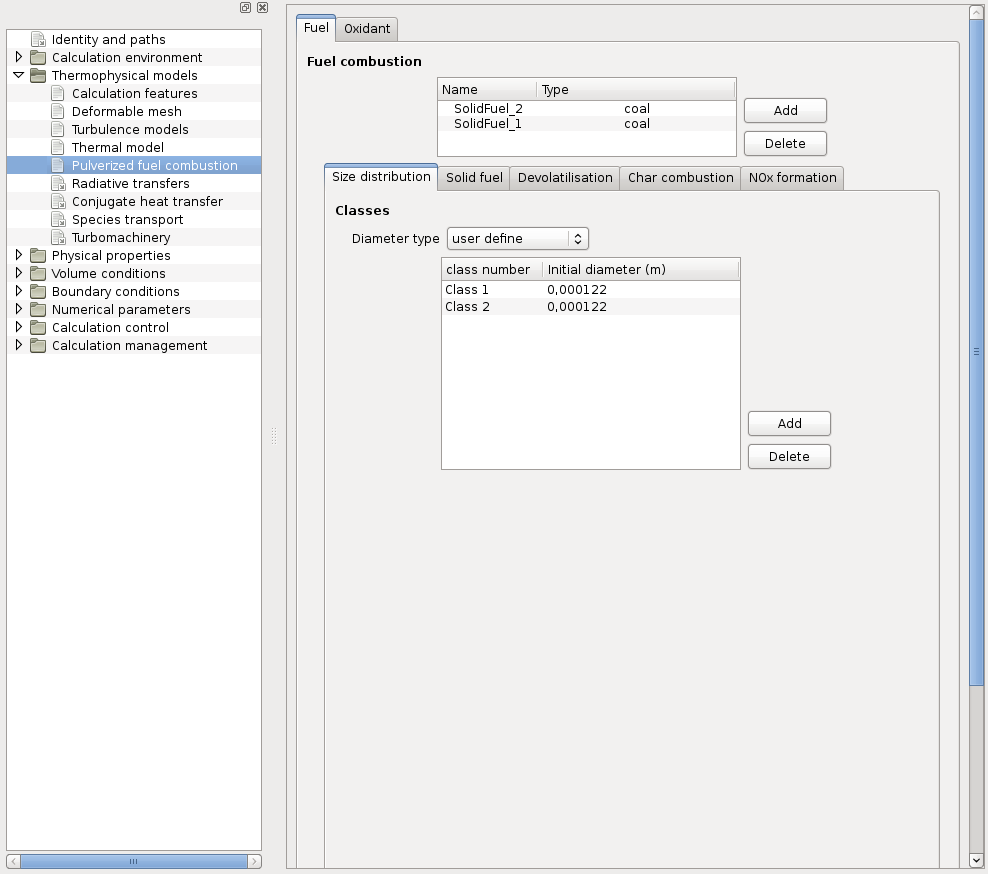
\includegraphics[width=12cm]{gui_coal_classes}
\caption{Thermophysical models - Pulverized coal combustion, coal classes}
\label{fig:Ini-coal1}
\end{center}
\end{figure}

\begin{figure}[!ht]
\begin{center}
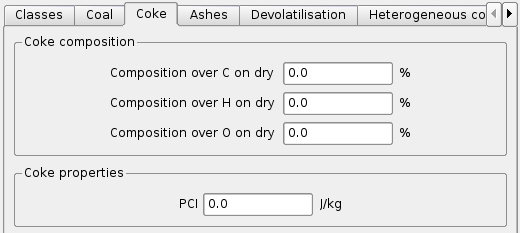
\includegraphics[width=11cm]{gui_coal_coke}
\caption{Pulverized coal combustion, coke}
\label{fig:Ini-coal2}
\end{center}
\end{figure}

\begin{figure}[!ht]
\begin{center}
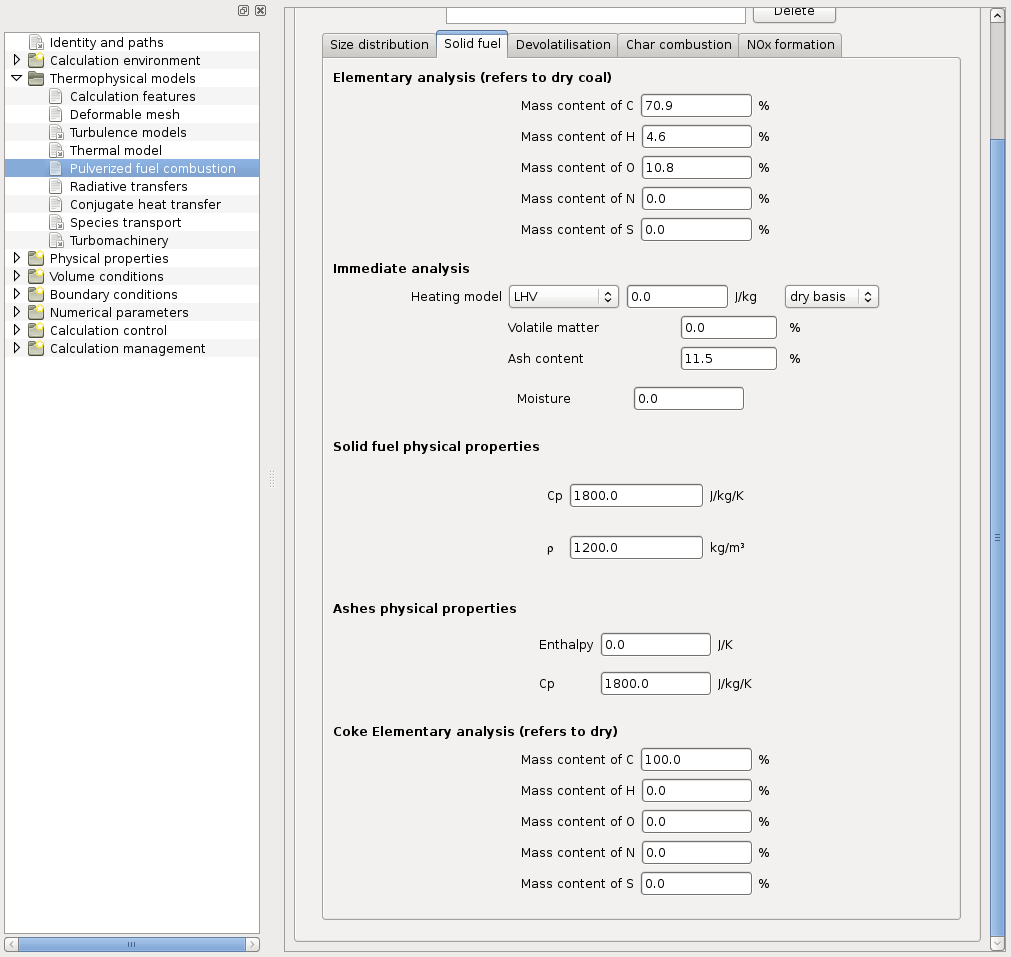
\includegraphics[width=11cm]{gui_coal_composition}
\caption{Pulverized coal combustion, coal composition}
\label{fig:Ini-coal3}
\end{center}
\end{figure}

\begin{figure}[!ht]
\begin{center}
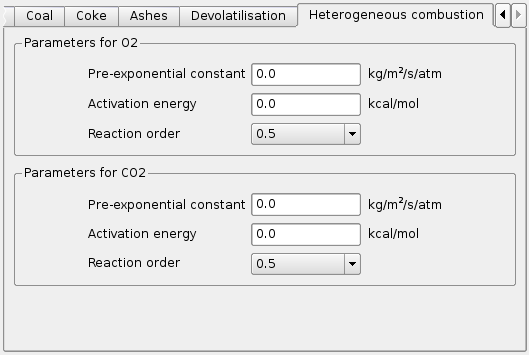
\includegraphics[width=11cm]{gui_coal_reaction}
\caption{Pulverized coal combustion, reaction parameters}
\label{fig:Ini-coal4}
\end{center}
\end{figure}

\begin{figure}[!ht]
\begin{center}
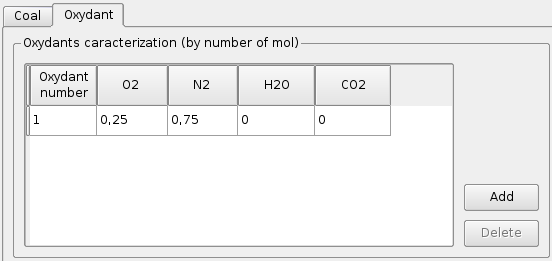
\includegraphics[width=11cm]{gui_coal_oxydant}
\caption{Pulverized coal combustion, oxydant}
\label{fig:Ini-coal5}
\end{center}
\end{figure}

If the user deals with gas combustion or if he (or she) does not want to use the GUI for coal combustion, the subroutines \texttt{usebui, usd3pi, uslwci} and \texttt{uscpiv} are used (only during the calculation initialisation).\\
In this section, ``specific physics'' will refer to gas combustion or
to pulverised coal combustion.

These subroutines allow the user to initialise some variables specific
to the specific physics activated {\em via} \texttt{usppmo}. As usual,
the user may have access to several geometric variables to discriminate
between different initialisation zones if needed.

{\em WARNING: in the case of a specific physics modeling, all the
variables will be initialised here, even the potential user scalars: {\em
\texttt{usiniv}} is no longer used.}


\begin{list}{$\bullet$}{}
       \item in the case of the EBU pre-mixed flame module, the user can
             initialise in every cell \texttt{iel}: the mixing rate
             \texttt{rtp\index{rtp}(iel,isca(ifm))} in variable richness, the
             fresh gas mass fraction \\
             \texttt{rtp(iel,isca(iygfm\index{iygfm}))}
             and the mixture enthalpy \texttt{rtp(iel,isca(ihm\index{ihm}))} in
             permeatic conditions

        \item in the case of the rapid complete chemistry diffusion flame
             module, the user can initialise in every cell \texttt{iel}: the
             mixing rate \texttt{rtp(iel,isca(ifm\index{ifm}))}, its variance
             \texttt{rtp(iel,isca(ifp2m\index{ifp2m}))} and the mixture mass
             enthalpy \texttt{rtp(iel,isca(ihm))} in permeatic conditions

        \item in the case of the pulverised coal combustion module, the
             user can initialise in every cell \texttt{iel}:
              \begin{list}{$\rightarrow$}{}
                     \item the transport variables related to the solid phase
                           \begin{list}{}{}
                                  \item \texttt{rtp(iel,isca(ixch\index{ixch}(icla)))} the reactive coal mass fraction related to the class \texttt{icla} (\texttt{icla} from 1 to \texttt{nclacp} which is the total number of classes, {\em i.e.} for all the coal type)
                                  \item \texttt{rtp(iel,isca(ixck(\index{ixck}icla)))} the coke mass fraction related to the class \texttt{icla}
                                  \item        \texttt{rtp(iel,isca(inp\index{inp}(icla)))} the number of particles related to class \texttt{icla} per kg of air-coal mixture
                                  \item \texttt{rtp(iel,isca(ih2\index{ih2}(icla)))} the mass enthalpy related to the class \texttt{icla} in permeatic conditions
                           \end{list}
                     \item \texttt{rtp(iel,isca(ihm))} the mixture enthalpy
                     \item the transport variables related to the gas phase
                           \begin{list}{}{}
                                  \item
                                       \texttt{rtp(iel,isca(if1m\index{if1m}(icha)))} the mean value of the tracer 1 representing the light volatile matters released by the coal \texttt{icha}
                                  \item
                                       \texttt{rtp(iel,isca(if2m\index{if2m}(icha)))} the mean value of the tracer 2 representing the heavy volatile matters released by the coal \texttt{icha}
                                  \item \texttt{rtp(iel,isca(if3m\index{if3m}))}
                                        the mean value of the tracer 3
                                        representing the carbon released
                                        as CO during coke burnout
                                  \item \texttt{rtp(iel,isca(if4p2m\index{if4p2m}))} the variance associated with the tracer 4 representing the air (the mean value of this tracer is not transported, it can be deduced directly from the three others)
                                  \item \texttt{rtp(iel,isca(ifp3m\index{ifp3m}))} the variance associated with the tracer 3
                           \end{list}
              \end{list}
\end{list}

%==================================
\subsubsection{Boundary conditions}\label{sec:coal-cl}
%==================================
In this section, ``specific physics'' refers to gas combustion or
to pulverised coal combustion.\\
For coal combustion, it is possible to manage the boundary conditions in the Graphical User Interface (GUI). When the coal combustion physics is selected in the heading ``Thermophysical models'', specific boundary conditions are activated for inlets, see fig. \ref{fig:cond_lim-coal}. The user fills for each type of coal previously defined (see Section \ref{sec:Ini-coal}) the initial temperature and initial composition of the inlet flow, as well as the mass flow rate.

\begin{figure}[!ht]
\begin{center}
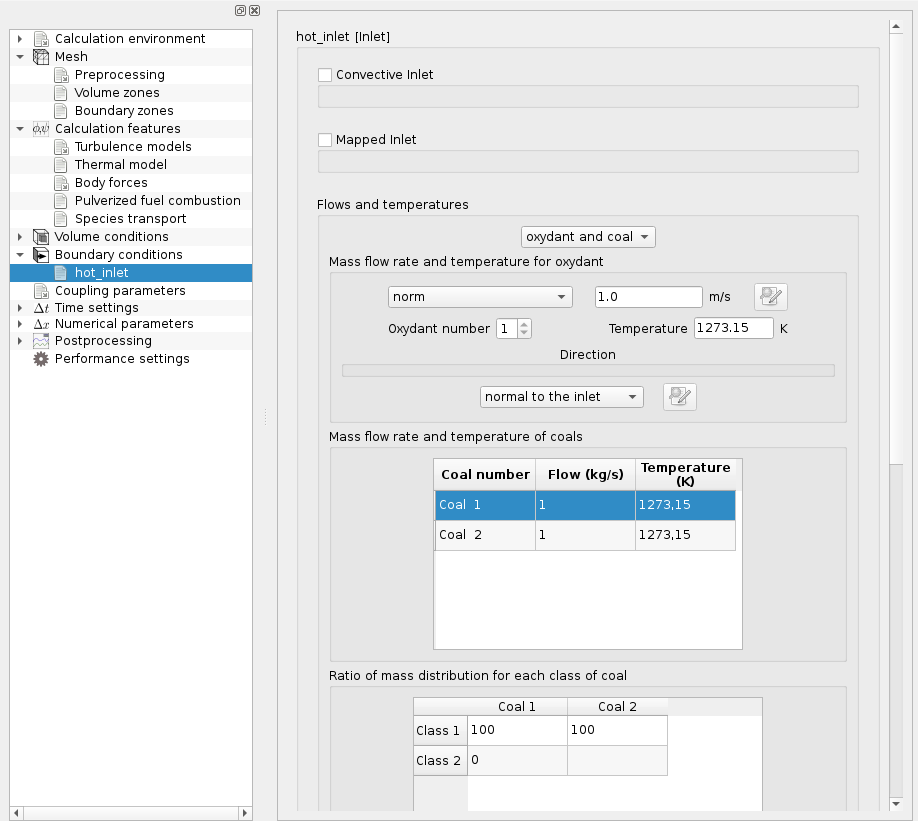
\includegraphics[width=13cm]{gui_coal_bc}
\caption{Boundary conditions for the combustion of coal}
\label{fig:cond_lim-coal}
\end{center}
\end{figure}

For gas combustion or if the GUI is not used for coal combustion, the use of \texttt{usebuc} (called at every time step),
\texttt {usd3pc}, \texttt{uslwcc}, \texttt{uscpcl} or \texttt{uscplc} is as
mandatory as \texttt{usini1} and \texttt{usppmo} to run a calculation involving specific physics. The way of using them is the same as using
\texttt{usclim} in the framework of standard calculations, that is, run several loops on the boundary faces lists (cf. \S\ref{fvm_selector})
marked out by their colors, groups, or  geometrical criterion, where
the type of face, the type of boundary condition for each variable and
eventually the value of each variable are defined.

{\em WARNING: In the case of a specific physics modeling, all the
boundary conditions for every variable must be defined here, even for
the eventual user scalars: {\em \texttt{usclim}} is not used at all.}\\

In the case of a specific physics modeling, a zone number \texttt{izone}
\footnote{\texttt{izone} must be less than the maximum number of boundary
zone allowable by the code, \texttt{nozppm}. This is fixed at 2000 in
 \texttt{pppvar.h};not to be modified} (for
instance the color \texttt{icoul}) is associated with every boundary face, in
order to gather together all the boundary faces of the same type. In
comparison to \texttt{usclim}, the main change from the user point of
view concerns the faces whose boundary conditions belong to the type
\texttt{itypfb=ientre\index{ientre}}:

\begin{list}{$\bullet$}{}
       \item for the EBU pre-mixed flame module:
             \begin{list}{$\rightarrow$}{}
                    \item the user can choose between the ``burned gas
                          inlet'' type (marked out by the burned gas indicator
                          \texttt{ientgb\index{ientgb}(izone\index{izone})}=1) and the
                          ``fresh gas inlet'' type (marked out by
                          the fresh gas indicator
                          \texttt{ientgf\index{ientgf}(izone)}=1)
                    \item for each inlet type (fresh or burned
                          gas), a mass flow or a velocity must be imposed:

                          \begin{list}{-}{}
                                 \item to impose the mass flow,
                                     \begin{list}{-}{}
                                       \item the user gives to
                                             the indicator
                                             \texttt{iqimp\index{iqimp}(izone)}
                                             the value 1,
                                       \item  the
                                             mass flow value is set in
                                             \texttt{qimp\index{qimp}(izone)}
                                             (positive value, in $kgs^{-1}$)
                                       \item finally he imposes the
                                             velocity vector direction
                                             by giving the components of
                                             a direction vector in
                                             \texttt{rcodcl\index{rcodcl}(ifac,iu\index{iu})}, \texttt{rcodcl(ifac,iv\index{iv})} and \texttt{rcodcl(ifac,iw\index{iw})}
                                     \end{list}

{\em WARNING:
\begin{list}{-}{}
\item the variable \texttt{qimp(izone)} refers to the mass flow across the whole
      zone \texttt{izone} and not across a boundary face (specifically for the axisymetric calculations, the inlet suface of the mesh must be broken up)
\item the variable \texttt{qimp(izone)} deals with the inflow across the area \texttt{izoz} and only across this zone;it is recomended to pay attention to the boundary conditions.
\item the velocity direction vector is neither necessarily normed, nor
      necessarily incoming.
\end{list}}

                                 \item to impose a velocity, the user
                                       must give to the indicator
                                       \texttt{iqimp(izone)} the value 0 and set
                                       the three velocity components (in
                                       $m.s^{-1}$) in
                                       \texttt{rcodcl(ifac,iu)},
                                       \texttt{rcodcl(ifac,iv)} and
                                       \texttt{rcodcl(ifac,iw)}
                          \end{list}
                    \item finally he specifies for each gas inlet type
                          the mixing rate \texttt{fment\index{fment}(izone)} and
                          the temperature \texttt{tkent\index{tkent}(izone)} in Kelvin
             \end{list}

       \item for the ``3 points'' diffusion flame module:
             \begin{list}{$\rightarrow$}{}
                    \item the user can choose between the ``oxydiser
                          inlet'' type marked out by
                          \texttt{ientox\index{ientox}(izone)}=1 and the ``fuel
                          inlet'' type marked out by
                          \texttt{ientfu\index{ientfu}(izone)}=1
                    \item concerning the input mass flow or the input
                          velocity, the method is the same as for the
                          EBU pre-mixed flame module
                    \item finally, the user sets the temperatures
                          \texttt{tinoxy\index{tinoxy}} for each oxydiser inlet
                          and \texttt{tinfue\index{tinfue}}, for each fuel inlet

{\em Note: In the standard version, only the cases with only one
                          oxydising inlet type and one fuel inlet type
                          can be treated. In particular, there must be
                          only one input temperature for the oxidiser
                          (\texttt{tinoxy}) and one input temperature for the
                          fuel (\texttt{tinfuel}).}
             \end{list}

       \item for the pulverised coal module:
             \begin{list}{$\rightarrow$}{}
                    \item the inlet faces can belong to the ``primary
                          air and pulverised coal inlet'' type, marked
                          out by \texttt{ientcp\index{ientcp}(izone)}=1, or to
                          the ``secondary or tertiary air inlet'' type,
                          marked out by \texttt{ientat\index{ientat}(izone)}=1
                    \item in a way which is similar to the process
                          described in the framework of the EBU module,
                          the user chooses for every inlet face to
                          impose the mass flow or not (\texttt{iqimp(izone)}=1 or
                          0). If the mass flow is imposed, the user
                          must set the air mass flow value
                          \texttt{qimpat\index{qimpat}(izone)}, its direction in
                          \texttt{rcodcl(ifac,iu)}, \texttt{rcodcl(ifac,iv)}
                          and \\ \texttt{rcodcl(ifac,iw)} and the incoming
                          air temperature \texttt{timpat\index{timpat}(izone)} in
                          Kelvin. If the velocity is imposed, he has to
                          set  \texttt{rcodcl(ifac,iu)}, \\
                          \texttt{rcodcl(ifac,iv)} and \texttt{rcodcl(ifac,iw)}.

                    \item if the inlet belongs to the ``primary air and
                          pluverised coal'' \texttt{type (ientcp(izone) = 1)} the
                          user must also define for each coal type \texttt{icha}:
                          the mass flow
                          \texttt{qimpcp\index{qimpcp}(izone,icha)}, the
                          granulometric distribution
                          \texttt{distch\index{distch}(izone,icha,iclapc)}
                          related to each class \texttt{iclacp}, and the
                          injection temperature
                          \texttt{timpcp\index{timpcp}(izone,icha)}

             \end{list}
\end{list}

%==================================
\subsubsection{Initialisation of the options of the variables}
%==================================
In the case of coal combustion, time averages, chronological records and listings follow-ups can be set in the Graphical User Interface (GUI) or in the subroutines \texttt{usebu1, usd3p1, uslwc1, uscpi1} and \texttt{uscpl1}. In the GUI, under the heading ``Calculation control'', additional variables appear in the list in the items ``Time averages'' and ``Profiles'', as well as in the item Volume solution control'', see figs. \ref{fig:t_average-coal} and \ref{fig:V_control-coal}.

\begin{figure}[!ht]
\begin{center}
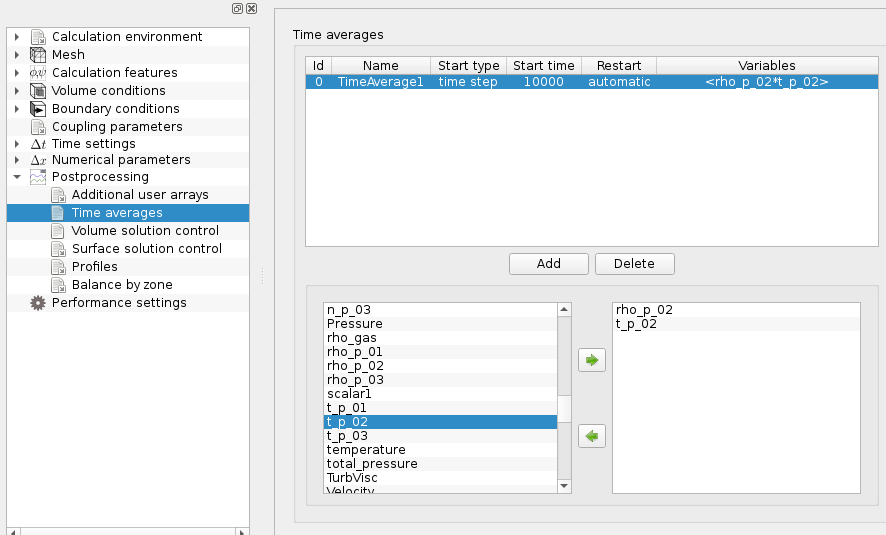
\includegraphics[width=12cm]{gui_coal_time_average}
\caption{Calculation control - Time averages}
\label{fig:t_average-coal}
\end{center}
\end{figure}

\begin{figure}[!ht]
\begin{center}
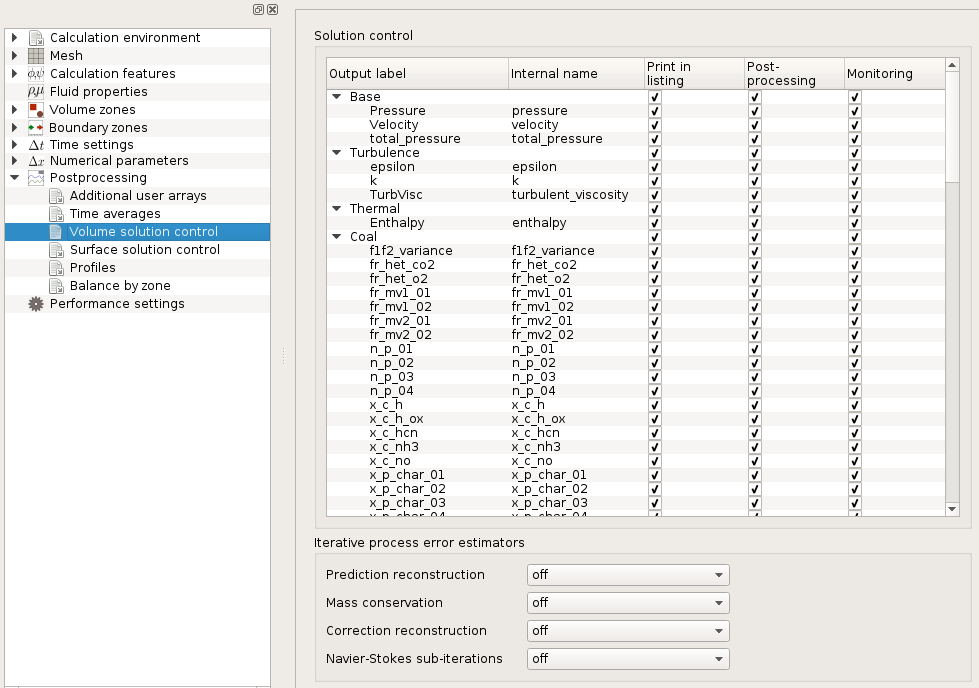
\includegraphics[width=13cm]{gui_coal_solution_control}
\caption{Calculation control - Volume solution control}
\label{fig:V_control-coal}
\end{center}
\end{figure}

In this section, ``specific physics'' refers to gas combustion or
pulverised coal combustion.

For gas combustion or if the GUI is not used for coal combustion, the 3 subroutines \texttt{usebu1, usd3p1, uslwc1, uscpi1} and \texttt{uscpl1} can be used to complete \texttt{usini1} for the
considered specific physics. These subroutines are called at the calculation start.
They allow to:
\begin{list}{$\bullet$}{}
\item generate, for the variables which are specific to the activated
             specific physics module, chronological outputs (indicators
             \texttt{ichrvr\index{ichrvr}(ipp)}), follow-ups in the listings
             (indicator \texttt{ilisvr\index{ilisvr}(ipp)}) and to activate
             chronological records at the probes defined in
             \texttt{usini1} (indicators \texttt{ihisvr(ipp)}).\\
The way of doing it is the same as in \texttt{usini1} and the writing
      frequencies of these ouputs are set by \texttt{usini1}. The values
      of the indicators \texttt{ipp} are
      \texttt{ipp=ipppro\index{ipppro}(ipproc\index{ipproc}(ivar))}, with \texttt{ivar}
      the number of the specific physics variable.
Concerning the main variables (velocity, pressure, etc ...) the user
      must still complete \texttt{usini1} if he wants to get
      chronological records, printings in the listing or chronological
      outputs.
The variables which can be activated by the user for each specific
      physics are listed below. The calculation variables \texttt{ivar} (defined
      at the cell \texttt{iel} by \texttt{rtp(iel,ivar)}) and the properties
      \texttt{iprop} (defined at the cell \texttt{iel} by
      \texttt{propce(iel,ipproc(iprop))}) are listed now:
      \begin{list}{$\rightarrow$}{}
       \item EBU pre-mixed flame modeling:
       \begin{list}{-}{}
        \item Calculation variables \texttt{rtp(iel,ivar)}
              \begin{list}{\texttt{ivar} = }{}
               \item \texttt{isca(iygfm\index{iygfm})} fresh gas mass fraction
               \item \texttt{isca(ifm\index{ifm})} mixing rate
               \item \texttt{isca(ihm\index{ihm})} enthalpy, if transported
              \end{list}
        \item Properties \texttt{propce(iel,ipproc(iprop))}
              \begin{list}{\texttt{iprop} = }{}
               \item \texttt{itemp\index{itemp}} temperature
               \item \texttt{iym(1)\index{iym(1)}} fuel mass fraction
               \item \texttt{iym(2)\index{iym(2)}} oxidiser mass fraction
               \item \texttt{iym(3)\index{iym(3)}} product mass fraction
               \item \texttt{ickabs\index{ickabs}} absorption
                     coefficient, when the radiation modeling is
                     activated
               \item \texttt{it3m\index{it3m}} and \texttt{it4m\index{it4m}}
                     ``$T^3$'' and ``$T^4$'' terms, when the radiation
                     modeling is activated
              \end{list}
       \end{list}
       \item rapid complete chemistry diffusion flame modeling:
             \begin{list}{}{}
              \item  everything is identical to the ``EBU'' case, except
                     the fresh gas mass fraction which is replaced by the
                     variance of the mixing rate \texttt{ivar=isca(ifp2m\index{ifp2m})}
             \end{list}
       \item pulverised coal modeling with 3 combustibles:
             \begin{list}{}{}
              \item {\em variables shared by the two phases}:
                    \begin{list}{-}{}
                     \item Calculation variables \texttt{rtp(iel,ivar)}
                           \begin{list}{\texttt{ivar} = }{}
                            \item \texttt{isca(ihm\index{ihm})}: gas-coal mixture enthalpy
                            \item \texttt{isca(immel\index{immel})}: molar mass of the
                                  gas mixture
                           \end{list}
                    \end{list}
              \item {\em variables specific to the dispersed phase}:
              \begin{list}{-}{}
               \item Calculation variables \texttt{rtp(iel,ivar)}
                     \begin{list}{\texttt{ivar} = }{}
                      \item \texttt{isca(ixck\index{ixck}(icla))}: coke mass
                            fraction related to the class \texttt{icla}
                      \item \texttt{isca(ixch\index{ixch}(icla))}: reactive coal
                            mass fraction related to the class \texttt{icla}
                      \item \texttt{isca(inp\index{inp}(icla))}: number of
                            particles of the class \texttt{icla} per kg of
                            air-coal mixture
                      \item \texttt{isca(ih2\index{ih2}(icla))}: mass enthalpy of
                            the coal of class \texttt{icla}, if we are in
                            permeatic conditions
                     \end{list}
               \item Properties \texttt{propce(iel,ipproc(iprop))}
                     \begin{list}{\texttt{iprop} = }{}
                      \item \texttt{immel\index{immel}}: molar mass of the gas mixture
                      \item \texttt{itemp2\index{itemp2}(icla)}: temperature of
                            the particles of the class \texttt{icla}
                      \item \texttt{irom2\index{irom2}(icla)}: density of
                            the particles of the class \texttt{icla}
                      \item \texttt{idiam2\index{idiam2}(icla)}: diameter of the
                            particles of the class \texttt{icla}
                      \item \texttt{igmdch\index{igmdch}(icla)}: disappearance
                            rate of the reactive coal of the class \texttt{icla}
                      \item \texttt{igmdv1\index{igmdv1}(icla)}: mass transfer
                            caused by the release of light volatiles
                            from the class \texttt{icla}
                      \item \texttt{igmdv2\index{igmdv2}(icla)}: mass transfer
                            caused by the release of heavy volatiles
                            from the class \texttt{icla}
                      \item \texttt{igmhet\index{igmhet}(icla)}: coke
                            disappearance rate during the coke burnout
                            of the class \texttt{icla}
                      \item \texttt{ix2\index{ix2}(icla)}: solid mass fraction
                            of the class \texttt{icla}
                     \end{list}
              \end{list}
              \item {\em variables specific to the continuous phase}:
              \begin{list}{-}{}
               \item Calculation variables \texttt{rtp(iel,ivar)}
                     \begin{list}{\texttt{ivar} = }{}
                      \item \texttt{isca(if1m\index{if1m}(icha))}: mean value of
                            the tracer 1 representing the light
                            volatiles released by the coal \texttt{icha}
                      \item \texttt{isca(if2m\index{if2m}(icha))}: mean value of
                            the tracer 2 representing the heavy
                            volatiles released by the coal \texttt{icha}
                      \item \texttt{isca(if3m)\index{if3m}}: mean value of the
                            tracer 3 representing the carbon released as
                            CO during coke burnout
                      \item \texttt{isca(if4pm\index{if4pm})}: variance of the
                            tracer 4 representing the air
                      \item \texttt{isca(if3p2m\index{if3p2m})}: variance of the
                            tracer 3
                     \end{list}
               \item Properties \texttt{propce(iel,ipproc(iprop))}
                     \begin{list}{\texttt{iprop} = }{}
                      \item \texttt{itemp1\index{itemp1}}: temperature of the gas
                            mixture
                      \item \texttt{iym1(1)\index{iym1(1)}}: mass fraction of
                            $CH_{X1m}$ (light volatiles) in the gas
                            mixture
                      \item \texttt{iym1(2)\index{iym1(2)}}: mass fraction of
                            $CH_{X2m}$ (heavy volatiles) in the gas
                            mixture
                      \item \texttt{iym1(3)\index{iym1(3)}}: mass fraction of
                            CO in the gas mixture
                      \item \texttt{iym1(4)\index{iym1(4)}}: mass fraction of
                            $O_2$ in the gas mixture
                      \item \texttt{iym1(5)\index{iym1(5)}}: mass fraction of
                            $CO_2$ in the gas mixture
                      \item \texttt{iym1(6)\index{iym1(6)}}: mass fraction of
                            $H_2O$ in the gas mixture
                      \item \texttt{iym1(7)\index{iym1(7)}}: mass fraction of
                            $N_2$ in the gas mixture
                     \end{list}
              \end{list}
             \end{list}
      \end{list}

 \item set the relaxation coefficient of the density \texttt{srrom}, with \\
$\rho^{n+1}=\texttt{srrom}*\rho^{n}+(1-\texttt{srrom})\rho^{n+1}$\\
(by default, the adopted value is \texttt{srrom\index{srrom}} = 0.8. At the
      beginning of a calculation, a sub-relaxation of 0.95 may reduce
      the numerical ``schocks'').

 \item set the dynamic viscosity \texttt{diftl0}. By default
      \texttt{diftl0\index{diftl0}}= 4.25 $kgm^{-1}s^{-1}$
(the dynamic diffusivity being the ratio between the thermal
      conductivity $\lambda$ and the mixture specific heat $C_p$ in the
      equation of enthalpy).

 \item set the value of the constant \texttt{cebu\index{cebu}} of the Eddy Break
      Up model (only in \texttt{usebu1}. By default \texttt{cebu}=2.5)
\end{list}

%==================================
\subsection{Heavy fuel oil combustion module}
%==================================
%==================================
\subsubsection{Initialisation of transported variables}
%==================================
To initialise or modify (in case of a continuation) values of transported variables and of the time step, the subroutine \texttt{usfuiv} is used. It is similar to \texttt{usiniv}. It is called at the beginning of every computation (new or continuation) before the time loop.

Physical properties are stored in \texttt{propce} (cell center), \texttt{propfa} (inner face) and \texttt{propfb}. For instance, \texttt{propce(iel, ipproc(irom  ))} is \texttt{rom(iel)}, the mean density (in $kg.m^{-3}$), and \texttt{propfa(ifac,ipprof(ifluma(ivar)))} is \texttt{flumas(IFAC,IVAR)}, the convective flux of the variable \texttt{ivar}.\\
Physical properties (\texttt{rom, viscl, cp, ...}) are computed in \texttt{ppphyv} and are not to be modified here.

All cells can be identified by using the subroutine '\texttt{getcel}'. All boundary faces may be identified using the '\texttt{getfbr}' subroutine. All internal faces may be identified using the '\texttt{getfac}' subroutine. Details of the syntax of these three subroutines are given in \texttt{usfuiv}.

In \texttt{usfuiv} the user initialise quantities related to the turbulent model chosen, and to gaseous species and droplets compositions. Exemples are provided in the subroutine.

%==================================
\subsubsection{Boundary conditions}
%==================================
Boundary conditions are defined on a per-face basis in \texttt{usfucl}. Boundary faces may be identified using the '\texttt{getfbr}' subroutine. \texttt{usfucl} is very similar to \texttt{uscpcl}, see Section \ref{sec:coal-cl}. Boundary conditions may be assigned in two ways:
\begin{list}{.}{}
\item for ``standard'' boundary conditions (inlet, free outlet, wall, symmetry): a code is defined in the array \texttt{itypfb} (of dimensions equal to the number of boundary faces). This code will then be used by a non-user subroutine to assign the conditions.
\item for ``non-standard'' conditions: see details given in \texttt{usfucl}.
\end{list}

%==================================
\subsubsection{Initialisation of the options of the variables}
%==================================

The presence of a fuel combustion module variable in the listing, {\itshape histo} files, and the output frequency are set in the subroutine \texttt{usfui1}. If the vectors below are not allocated, default values will be used:
\begin{list}{-}{}
\item \texttt{ichrvr}: chronological output (1:yes / 0:no)
\item \texttt{ilisvr}: listing output (1:yes / 0:no)
\item \texttt{ihisvr}: {\itshape histo} output (number of probes and probe numbers), if $= -1$, every probes defined in \texttt{usini1} will be found in the {\itshape histo} files
\end{list}

Calculation options such as a the relaxation parameter the for density (recommended when starting a combustion computation but forbidden for unstationnary computations) can also be set, as well as physical constants like the the laminar viscosity for the enthalpy.

%==================================
\subsection{Radiative thermal transfers in semi-transparent gray media}
%==================================
%==================================
\subsubsection{Initialisation of the radiation main parameters}
%==================================

The main radiation parameters can be initialise in the Graphical User Interface (GUI) or in the user subroutine \texttt{usray1}. In the GUI, under the heading ``Thermophysical models'', when one of the two thermal radiative transfers models is selected, see fig. \ref{fig:0_ray}, additional items appear. The user is asked to choose the number of directions for angular discretisation, to define the absorption coefficient and select if the radiative calculation are restarted or not, see figs. \ref{fig:1_ray} and \ref{fig:3_ray}. When ``Advanced options'' is selected for both models figs. \ref{fig:2_ray} or \ref{fig:4_ray} appear, the user must fill the resolution frequency and verbosity levels. In addition, the activation of the radiative transfer leads to the creation of an item ``Surface solution control'' under the heading ``Calculation control'', see fig. \ref{fig:5_ray}, where radiative transfer variables can be selected to appear in the output listing.

\begin{figure}[ht]
\begin{center}
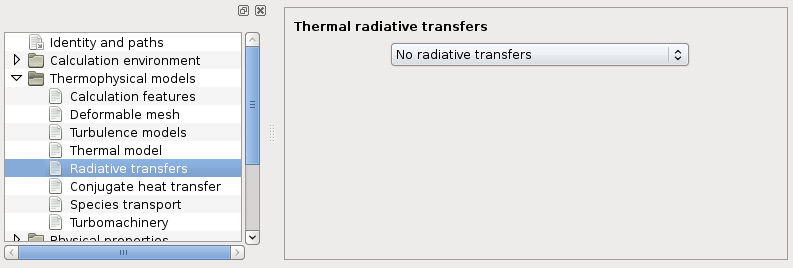
\includegraphics[width=13cm]{gui_rad_transf_models}
\caption{Radiative transfers models}
\label{fig:0_ray}
\end{center}
\end{figure}

\begin{figure}[ht]
\begin{center}
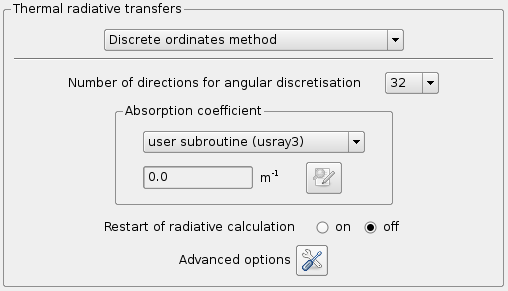
\includegraphics[width=10cm]{gui_rad_transf_do_params}
\caption{Radiative transfers - parameters of the DO method}
\label{fig:1_ray}
\end{center}
\end{figure}

\begin{figure}[ht]
\begin{center}
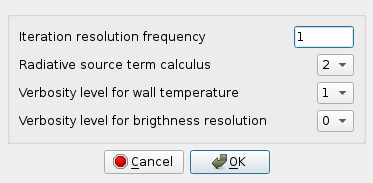
\includegraphics[width=7cm]{gui_rad_transf_do_advanced}
\caption{Radiative transfers - advanced parameters of the DO method}
\label{fig:2_ray}
\end{center}
\end{figure}

\begin{figure}[ht]
\begin{center}
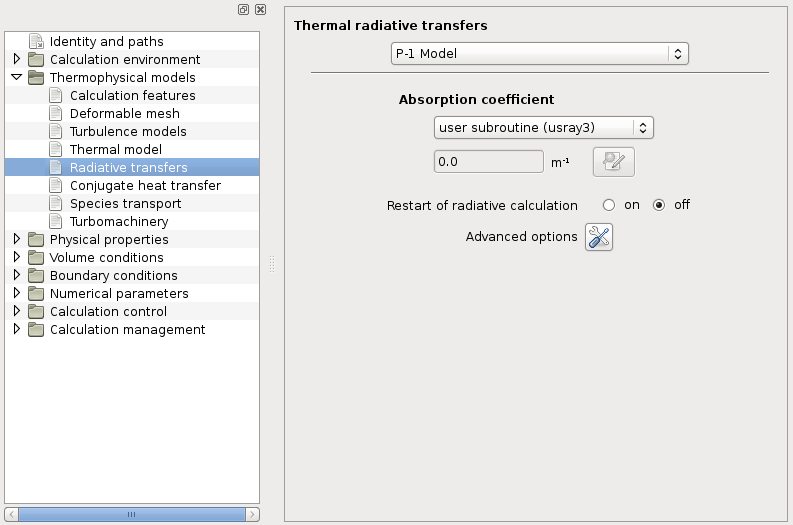
\includegraphics[width=10cm]{gui_rad_transf_p1_params}
\caption{Radiative transfers - parameters of the P-1 model}
\label{fig:3_ray}
\end{center}
\end{figure}

\begin{figure}[ht]
\begin{center}
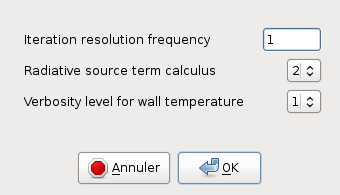
\includegraphics[width=7cm]{gui_rad_transf_p1_advanced}
\caption{Radiative transfers - advanced parameters of th P-1 model}
\label{fig:4_ray}
\end{center}
\end{figure}

\begin{figure}[ht]
\begin{center}
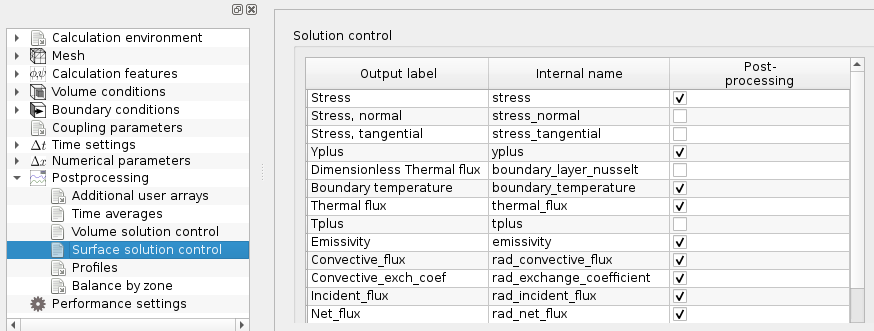
\includegraphics[width=6cm]{gui_rad_transf_post_output}
\caption{Calculation control - Radiative transfers postprocessign output}
\label{fig:5_ray}
\end{center}
\end{figure}

If the GUI is not used, \texttt{usray1} is one of the two subroutine which must be completed by the user for all
calculations including radiative thermal transfers. It is called only during the calculation initialisation. It is composed of three headings. The first one is dedicated to the activation
of the radiation module, only in the case of classic physics. \\
{\em WARNING: when a calculation is ran using a specific physics module,
this first heading must not be completed. The radiation module is then
activated or not, according to the parameter file related to the considered
specific physics.} \\

\noindent
In the second heading the basic parameters of the radiation module are indicated.\\
Finally, the third heading deals with the selection of the
post-processing graphic outputs. The variables to treat are splitted
into two categories: the volumetric variables and those related to the
boundary faces.\\

\noindent
For more details about the different parameters, the user may refer to the
key word list (\S\ref{prg_motscles}).


%==================================
\subsubsection{Radiative transfers boundary conditions}
%==================================
These informations can be filled by the user through the Graphical User Interface (GUI) or by using the subroutine \texttt{usray2} (called every time step). If the interface is used, when one of the ``Radiative transfers'' options is selected in fig. \ref{fig:0_ray}, it activates specific boundary conditions each time a ``Wall'' is defined, see fig. \ref{fig:6_ray}. The user can then choose between 3 cases. The parameters the user must specify are displayed for one of them in fig. \ref{fig:7_ray}.
 
\begin{figure}[ht]
\begin{center}
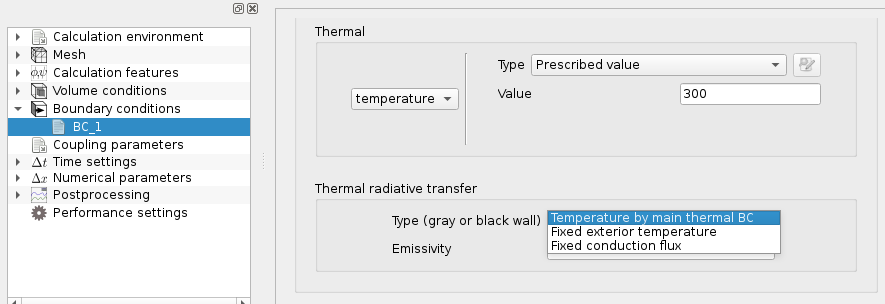
\includegraphics[width=11cm]{gui_rad_transf_wall_model}
\caption{Boundary conditions - choice of wall thermal radiative transfers}
\label{fig:6_ray}
\end{center}
\end{figure}

\begin{figure}[ht]
\begin{center}
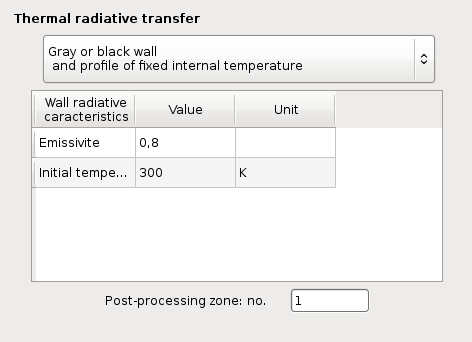
\includegraphics[width=11cm]{gui_rad_transf_wall_params}
\caption{Boundary conditions - example of wall thermal radiative transfer}
\label{fig:7_ray}
\end{center}
\end{figure}

When the GUI is not used, \texttt{usray2} is the second subroutine necessary for every calculation which includes radiative thermal transfers. It is used to give all the
necessary parameters concerning, in the one case, the wall temperature
calculation, and in the other, the coupling between the thermal
scalar (temperature or enthalpy), and the radiation module at the
calculation domain boundaries. It must be noted that the boundary conditions
concerning the thermal scalar which may have been defined in the
subroutine \texttt{usclim} will be modified by the radiation module
according to the data given in \texttt{usray2} (cf. \S\ref{fvm_selector}).\\
A zone number must be given to each boundary face \footnote{this must be less
 than the maximum allowable by the code, \texttt{nozrdm}. This is fixed at 2000
 in \texttt{radiat.h} and cannot be modified.}and, specifically for
the walls, a boundary condition type and an initialisation temperature
(in Kelvin). The initialisation temperature is only used to make the
solving implicit at the first time step. The zone number allows to assign
an arbitrary integer to a set of boundary faces having the same
radiation boundary condition type. This gathering is used by the
calculation, and in the listing to print some physical values (mean
temperature, net radiative flux ...). An independent graphic output in
{\em EnSight} format is associated with each zone and allows the display on
the boundary faces of the variables selected in the third heading of the
subroutine \texttt{usray1}.\\
A boundary condition type stored in the array ISOTHP is associated with
each boundary face. There are five different types:

\begin{list}{$\bullet$}{}

\item \texttt{\textbf{itpimp}}: wall face with imposed temperature,

\item \texttt{\textbf{ipgrno}}: for a gray or black wall face, calculation of the
      temperature by means of a flux balance,

\item \texttt{\textbf{iprefl}}: for a reflecting wall face, calculation of the
      temperature by means of a flux balance.
 This is fixed at 2000 in \texttt{radiat.h} and cannot be modified.

\item \texttt{\textbf{ifgrno}}: gray or black wall face to which a conduction
      flux is imposed,

\item \texttt{\textbf{ifrefl}}: reflecting wall face to which a conduction
      flux is imposed, which is equivalent to impose this flux directly
      to the fluid.

\end{list}

\noindent
Depending on the selected boundary condition type at every wall face,
the code needs to be given some supplementary pieces of information:

\begin{list}{$\bullet$}{}

\item \texttt{\textbf{itpimp}}: the array \texttt{tintp} must be completed
      with the imposed temperature value and the array \texttt{epsp} must
      be completed with the emissivity value (strictly positive).

\item \texttt{\textbf{ipgrno}}: must be given: an initialisation temperature in
      the array \texttt{tintp}, the wall emissivity (strictly positive, in
      \texttt{epsp}), thickness (in \texttt{epap}), thermal conductivity
      (in \texttt{xlamp}) and an external temperature (in \texttt{textp})
      in order to calculate a conduction flux across the wall.

\item \texttt{\textbf{iprefl}}: must be given: an initialisation temperature (in
      \texttt{tintp}), the wall thickness (in \texttt{epap}) and thermal conductivity (in
      \texttt{xlamp}) and an external temperature (in \texttt{textp}).

\item \texttt{\textbf{ifgrno}}: must be given: an initialisation temperature (in
      \texttt{tintp}), the wall emissivity (in \texttt{epsp}) and the conduction
      flux (in $W/m^2$ whatever the thermal scalar, enthalpy or temperature) in
      the array \texttt{rcodcl}. The value of \texttt{rcodcl} is positive when the
      conduction flux is directed from the inside of the fluid domain to the
      outside (for instance, when the fluid heats the walls). If the
      conduction flux is null, the wall is adiabatic.

\item \texttt{\textbf{ifrefl}}: must be given: an initialisation temperature (in
      \texttt{tintp}) and the conduction flux (in $W/m^2$ whatever the thermal
      scalar) in the array \texttt{rcodcl}. The value of \texttt{rcodcl} is
      positive when the conduction flux is directed from the inside of the
      fluid domain to the outside (for instance, when the fluid heats the
      walls). If the conduction flux is null, the wall is adiabatic. The flux
      received by \texttt{rcodcl} is directly imposed as boundary condition for
      the fluid.

\end{list}

\noindent
{\em WARNING: it is mandatory to set a zone number to every boundary
face, even those which are not wall faces. These zones will be used during the
printing in the listing. It is recommended to gather together the
boundary faces of the same type, in order to ease the reading of the
listing.}\\

%==================================
\subsubsection{Absorption coefficient of the medium, boundary conditions
   for the luminance and calculation of the net radiative flux}
%==================================
When the absorption coefficient is not constant, the subroutine \texttt{usray3} is called instead at each time step. It is composed of three parts. In the first one, the user
must provide the absorption coefficient of the medium in the array CK,
for each cell of the fluid mesh. By default, the absorption coefficient
of the medium is 0, which corresponds to a transparent medium.\\

{\em WARNING: when a specific physics is activated, it is forbidden to
give a value to the absorption coefficient in this subroutine. In this
case, it is calculated automatically, or given by the user {\em via} a
thermo-chemical parameter file (dp\_C3P or dp\_C3PSJ for gas combustion,
and dp\_FCP for pulverised coal combustion).}\\

\noindent
The two following parts of this subroutine concern a more advanced use
of the radiation module. It is about imposing boundary conditions to the
equation of radiative transfer and net radiative flux calculation, in
coherence with the luminance at the boundary faces, when the user wants
to give it a particular value. In most cases, the given examples do not
need to be modified.

%==================================
\subsubsection{Encapsulation of the temperature-enthalpy conversion}
%==================================

\noindent
\textit{Subroutine called every time step.}

The user subroutine \texttt{usray4} is used to call the user subroutine \texttt{usthht}. \texttt{usthht} is used to encapsulate a simple enthalpy-temperature
conversion law and its inverse. The user
can implement his own conversion formulas into it. \\
This subroutine is useless when the thermal scalar is the temperature.\\
\noindent

{\em WARNING: when a specific physics is activated, it is forbidden to use this
subroutine. In this case, {\em \texttt{usray4}} is replaced by {\em
\texttt{ppray4}}, which is not a user subroutine.}\\

\noindent
The value of the argument \texttt{mode} allows to know in which direction the
conversion will be made:
\begin{list}{$\bullet$}{}

\item \texttt{\textbf{mode = 1}}: the fluid enthalpy in the cell must be
      converted into temperature (in Kelvin),

\item \texttt{\textbf{mode = -1}}: the wall temperature (\texttt{text}
      or \texttt{tparoi}, in Kelvin) must be converted into enthalpy.

\end{list}
%
{\em WARNING: the value of \texttt{mode} is passed as argument and must not be
modified by the user.}\\

%==================================
\subsubsection{Input of radiative transfer parameters}
%==================================

\noindent
\textit{The routine \texttt{usray5} is called twice. The first time is for boundary 
conditions. The second time is for the net radiation flux computation}

In this subroutine, during the first call (\texttt{iappel=1}), the boundary conditions
 are filled:
\begin{list}{-}{}
\item the radiative intensity must be set in the array \texttt{cofrua} when the discrete
 ordinates model is used; an example is given in \texttt{usray5} for an isotropic radiation
 field on a gray wall. Proposed boundary conditions for the intensity in \texttt{usray5} are: 
symmetry, inlet/oulet, and wall boundary,
\item the entering intensity for free boundaries is set to zero in \texttt{cofrua} (if the 
user has more information, he can improve it),
\item arrays \texttt{cofrua} and \texttt{cofrub} must be filled when the P-1 model is
 used. The boundary conditions proposed are the same as with the discret ordinates model.
\end{list}
During the second call (\texttt{iappel=2}), the density of the net radiation flux must be
 calculated consistently with the boundary conditions of the intensity considering that the 
density of net flux is the balance between the radiative emiting part of a boundary face 
(and not the reflecting one) and the radiative absorbing part. The provided example is 
consistent with the example of the intensity boundary conditions given when the discret
 ordinates model is used.


%==================================
\subsection{Conjugate heat transfers}
%==================================
%========================================
\subsubsection{Thermal module in a 1D wall}
%========================================

\noindent
\textit{subroutine called at every time step}

This subroutine takes into account the affected thermal inertia by a wall.
 Some boundary faces are treated as a solid wall with a given thickness, on
 which the code resolves an undimensional equation for the heat conduction.
 The coupling between the 1D module and the fluid works in a similar way to
 the coupling with the \syrthes. In construction, the user is not able to
 account for the heat transfer between different parts of the wall. A physical
 analysis of each problem, case by case is required to evaluate the relevance
 of its usage by way of a report of the simple conditions (temperature, zero-flux
 ) or a coupling with \syrthes.\\

The use of this code requires that the thermal scalar is
defined as (\texttt{iscalt}$>0$).

{\em WARNING: The 1D thermal module is developped assuming the thermal scalar
 as a temperature. If the thermal scalar is an enthalpy, the code calls the
 subroutine \texttt{usthht} for each transfer of information between the fluid
 and the wall in order to convert the enthalpy to temperature and vice-versa.
 This function has not been tested and is firmly discouraged. If the thermal
 variable is the total (compressible) energy, the thermal module will not work.}

\bigskip

This procedure  is called twice,on initialisation and again at each time step.

\begin{list}{$\bullet$}{}
\item The 1st call (initialisation) all the boundary faces that will be treated
 as a coupled wall are marked out. This figure is written noted as
 \texttt{nfkpt1d}. It applies dimension to the arrays in the thermal module.
 \texttt{nfkpt1d} will be at 0 if there are no coupled faces (it is in fact the
 default value, the remainer of the subroutine is not used in this case).
 The parameter \texttt{isuit1} also need to be defined, this indicates if the
 temperature of the wall must be initialised or written in the file (stored in
 the variable \texttt{filmt1}).
\item The 2nd call (initialisation) again concern the wall faces, it completes
 the \texttt{ifpt1d} array of dimension \texttt{nfpt1d}.
 \mbox{\texttt{ifpt1d(ifbt1d)}} is the number
 \texttt{ifbt1d}\raisebox{1ex}{\small th} boundary faces coupled with the thermal module
 of a 1D wall. The directional parameters are then completed for a pseudo
 wall associated to each face
\begin{list}{-}{}
\item \texttt{nppt1d(nfpt1d)\index{nppt1d}}: number of cells in the 1D mesh associated
 to the pseudo wall.
\item \texttt{eppt1d(nfpt1d)\index{eppt1d}}: thickness of the pseudo wall.
\item \texttt{rgpt1d(nfpt1d)\index{rgpt1d}}: geometery of the pseudo wall mesh (refined
 as a fluid if \texttt{rgt1d} is smaller than 1)
\item \texttt{tppt1d(nfpt1d)\index{tppt1d}}: initialisation temperature of the wall
(uniform in thickness). In the course of the calculation, the array stores the
 temperature of the solid at the fluid/solid interface.
\end{list}

Other than for re-reading a file (\texttt{ficmt1}), \texttt{tppt1d} is not used.
\texttt{nppt1d}, \texttt{ifpt1d}, \texttt{rgpt1d} and \texttt{eppt1d} are
compared to data from the follow-up file and they must be identical.

{\em WARNING: The test in \texttt{ifpt1d} implicilty assumes that the array is completed
 in ascending order (i.e \texttt{ifpt1d(ii)}$>$\texttt{ifpt1d(jj)} if ii$>$jj.
 This will be the case if the coupled faces are defined starting from the unique loop on the
boundary faces (as in the example). If this is not the case, contact the development
 team to short circuit the test.}

\item The 3rd call (at each time step) is for the confirmation that all the arrays
 involving physical parameter and external boundary conditions have been completed.
\begin{list}{-}{}
\item \texttt{iclt1d(nfpt1d)\index{iclt1d}}:Typical boundary condition at the external
 (pseudo) wall: Dirichlet condition (\texttt{iclt1d}=1) or flux condition (\texttt{iclt1d}=3)
\item \texttt{tept1d(nfpt1d)\index{tept1d}}: External temperature of the pseudo wall in the
 Dirichlet case.
\item \texttt{hept1d(nfpt1d)\index{hept1d}}: External coefficient of transfer in the pseudo
 wall under Dirichlet conditions (in $W.m^{-2}.K^.$).
\item \texttt{fept1d(nfpt1d)\index{nfpt1d}}: External heat flux in the pseudo wall under
 the flux conditions(in $W.m^{-2}$, negative value for energy entering the wall).
\item \texttt{xlmt1d(nfpt1d)\index{xlmt1d}}: Conductivity$\lambda$ of the wall uniform
in thickness (in $W.m^{-1}.K^{-1}$).
\item \texttt{rcpt1d(nfpt1d)\index{rcpt1d}}: Volumetric heat capacity $\rho C_p$ of the
wall uniform in thickness (in $J.m^{-3}.K^{-1}$).
\item \texttt{dtpt1d(nfpt1d)\index{dtpt1d}}: Physical time step ascociated with the solved
 1D equation of the pseudo wall(which can be different from the time step in the
 calculation).
\end{list}

\end{list}

The $3^{rd}$ call, done at each time step, allows to impose boundary conditions
 and physical values in time.

%==================================
\subsubsection{Fluid-Thermal coupling with \syrthes}
%==================================
When the user wishes to couple \CS with \syrthes to include heat transfers, it can be 
done in the Graphical User Interface (GUI) or in the user subroutine
\texttt{cs\_syrthes\_coupling}.
In the GUI, to set such a coupling, a thermal scalar must be 
selected first in the item ``Thermal scalar'' under the heading ``Thermophysical models''.
 Then the item ``Conjugate heat transfer'' will appear, see fig. \ref{fig:syrthes}.
 The zones where the coupling occurs must be defined and a projection axis can be 
specified in case of 2D coupling.

\begin{figure}[ht]
\begin{center}
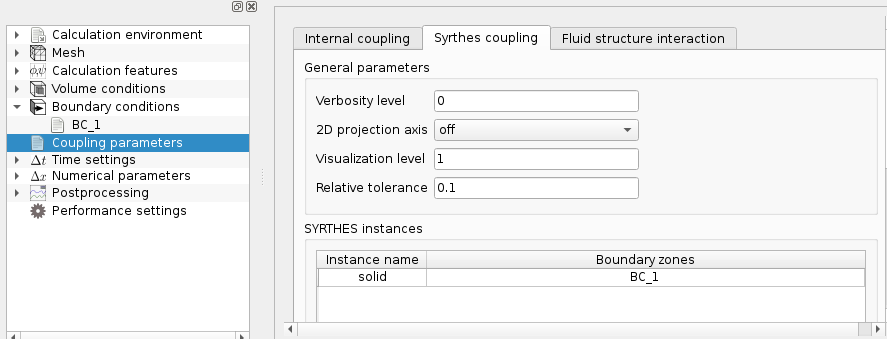
\includegraphics[width=8cm]{gui_syrthes_coupling}
\caption{Thermophysical models - coupling with \syrthes}
\label{fig:syrthes}
\end{center}
\end{figure}

If the subroutine \texttt{ussyrc} is used, the user must specify the arguments 
passed to the subroutine '\texttt{defsyr}'. These arguments are:
\begin{list}{-}{}
 \item \texttt{numsyr} is the matching \syrthes application \texttt{id} number, or $-1$,
 \item \texttt{namsyr} is the matching \syrthes application name,
 \item \texttt{cprjsy}: ' ' if the user wishes to use a 3D standard coupling,
 or specify '$x$', '$y$', or '$z$' as the projection axis if a 2D coupling with \syrthes is used,
 \item \texttt{critsu} is the surface selection criteria,
 \item \texttt{critvl} is the volume selection criteria (only with \syrthes 4),
 \item \texttt{iwarns} is the verbosity level.
\end{list}
Examples are provided in '\texttt{ussyrc}'.


%==================================
\subsection{Lagrangian modeling of multiphase flows with dipersed inclusions}
%==================================

%==================================
\subsubsection{Initialisation  of the Lagrangian
   modeling parameters}\label{sec:Ini-lag}
%==================================

The initialisation of the Lagrangian module parameters can be performed in
 the Graphical User Interface (GUI) or in the user subroutine \texttt{uslag1} 
(called only during the calculation initialisation). In the GUI, the selection
 of the Lagrangian module in the item ``Calculation features'' under the heading
 ``Thermophysical models'' activates the heading ``Particle and droplets 
tracking''. The initialisation is performed in the three items included in 
this heading. In ``Global settings'', the user defines the Eulerian/Lagrangian 
multi-phase treatment, the main parameters, the specific physics associated with
 the particles and numerical adavanced options, see figs. \ref {fig:Ini-Lag1}
 to \ref {fig:Ini-Lag3}. In the item ``Statistics'', names are associated to 
volume and boundary statistical variables for listing and post-processing, 
see fig. \ref {fig:Ini-Lag4}. In the item ``Output'', the user defines the
 output frequency, post-precessing options for particles and selects the variables
 that will appear in the listing, see.fig. \ref {fig:Ini-Lag5}.

\begin{figure}[ht]
\begin{center}
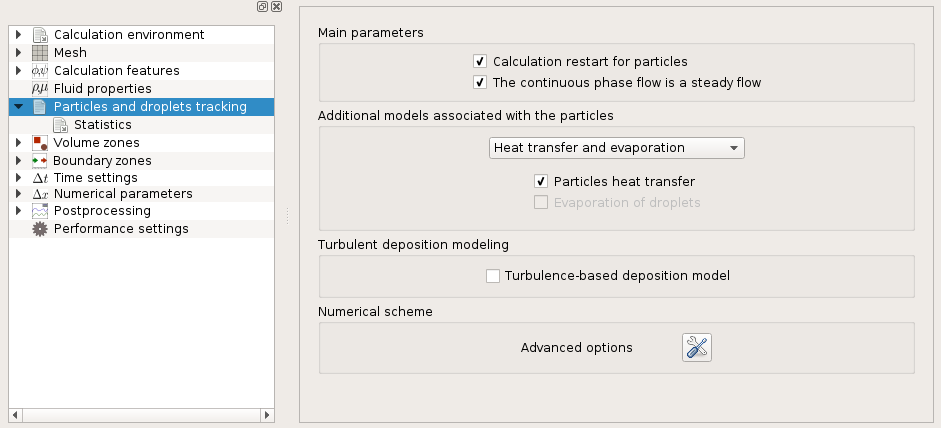
\includegraphics[width=12cm]{gui_lagr_global_settings}
\caption{Lagrangian module - global settings}
\label{fig:Ini-Lag1}
\end{center}
\end{figure}

\begin{figure}[ht]
\begin{center}
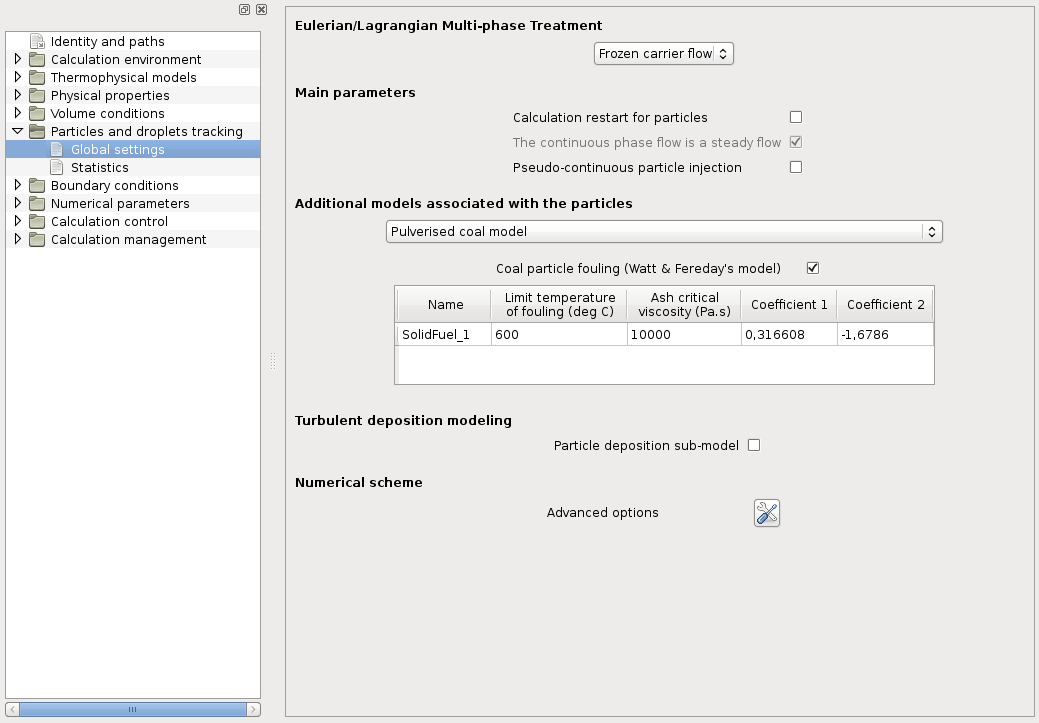
\includegraphics[width=10cm]{gui_lagr_global_settings_coal}
\caption{Lagrangian module - global settings, specific physics}
\label{fig:Ini-Lag2}
\end{center}
\end{figure}

\begin{figure}[ht]
\begin{center}
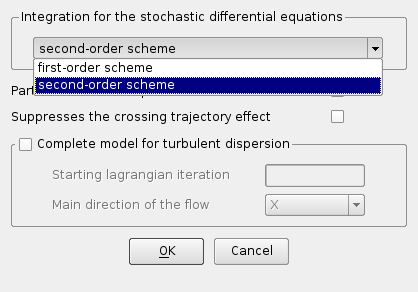
\includegraphics[width=8cm]{gui_lagr_global_advanced}
\caption{Lagrangian module - global settings, advanced numerical options}
\label{fig:Ini-Lag3}
\end{center}
\end{figure}

\begin{figure}[ht]
\begin{center}
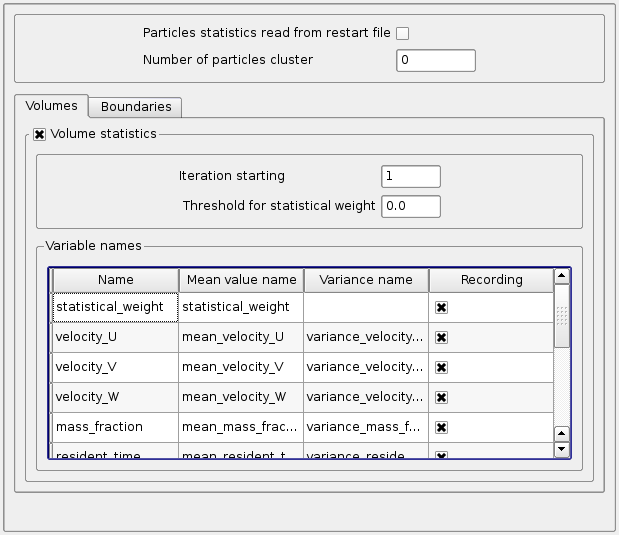
\includegraphics[width=11cm]{gui_lagr_statistics}
\caption{Lagrangian module - statistics}
\label{fig:Ini-Lag4}
\end{center}
\end{figure}

\begin{figure}[ht]
\begin{center}
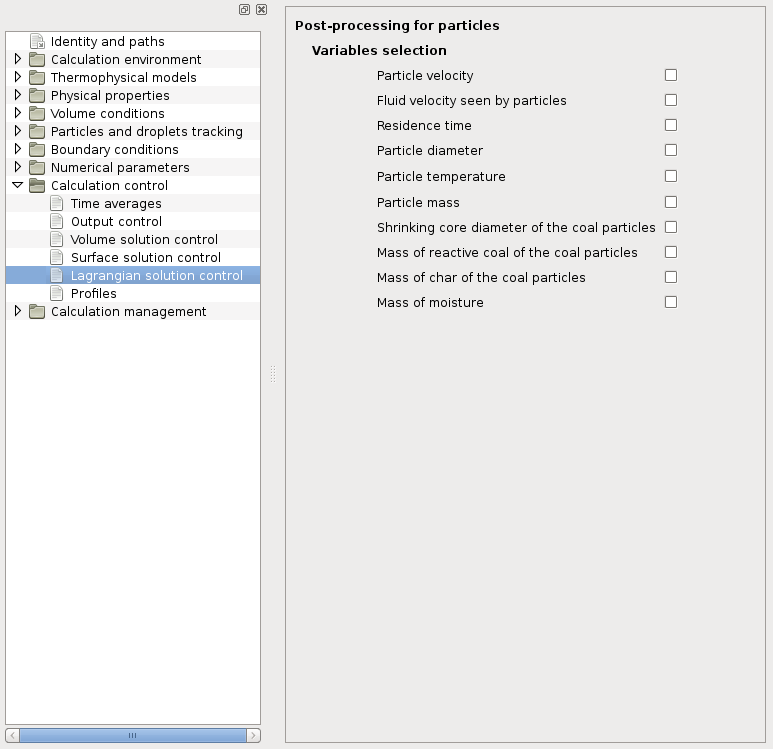
\includegraphics[width=11cm]{gui_lagr_output}
\caption{Lagrangian module - output}
\label{fig:Ini-Lag5}
\end{center}
\end{figure}

\noindent
When the GUI is not used, \texttt{uslag1} is one of the two subroutines which must be completed in
the case of a calculation using a Lagrangian multiphase flow model. This
subroutine gathers in different headings all the key word which are
necessary to configure the Lagrangian module. The different headings
refer to:
\begin{list}{$\bullet$}{}
\item the global configuration parameters
\item the specific physical models describing the particle behaviour
\item the backward coupling (influence of the dispersed phase on the
      continuous phase)
\item the numerical parameters
\item the volumetric statistics
\item the boundary statistics
\item the postprocessing in trajectory mode
\end{list}
%
\noindent
For more details about the different parameters, the user may refer to the
key word list (\S\ref{prg_motscles_lagr}).

\noindent
The results of the lagangian module consist in some information about
the particle cloud. These pieces of information are displayed in the
form of statistics. It is therefore necessary to activate the
calculation of the statistics at a given instant during the
simulation. To do so, there are different strategies which are strongly
related to the flow nature, stationary or not. \\
Except from the cases where the injection conditions depend on the time,
it is generally recommended to realise a first Lagrangian calculation
whose aim is to get a nearly constant particle number in the calculation
domain. In a second step, a calculation restart is done to calculate the
statistics. \\
When the single-phase flow is steady and the inclusion presence rate
is low enough to neglect their influence on the continuous phase
behaviour, it is better to realise a Lagrangian calculation on a fixed
field. It is then possible to calculate stationary volumetric statistics and
to give a statistical weight higher than 1 to the particles, in order to
reduce the number to treat while keeping the right concentrations. \\
Otherwise, when the continuous phase flow is stationary, but the backward
coupling must be taken into consideration, it is still possible to
activate stationary statistics. \\
When the continuous phase flow is non-stationary, it is no longer possible
to use stationary statistics. To have correct statistics at every moment
in the whole calculation domain, it is imperative to have an established
particle seeding and it is recommended (when it is possible) not to
impose statistical weights different from the unity. \\
Finally, when the complete model is used for the turbulent dispersion
modeling, the user must make sure that the volumetric statistics are
directly used for the calculation of the locally undisturbed fluid flow
field. \\
\noindent
When the thermal evolution of the particles is activated, the associated
particulate scalars are always the inclusion temperature and the locally
undisturbed fluid flow
temperature expressed in degrees Celsius, whatever the thermal scalar
associated with the continuous phase is (temperature or enthalpy). If the
thermal scalar associated with the continuous phase is the temperature
in Kelvin, the unit change is done automatically. If the
thermal scalar associated with the continuous phase is the enthalpy, the
enthalpy-temperature conversion subroutine \texttt{usthht} must be
completed for \texttt{mode}=1, and must express temperatures in degrees
Celsius. \\
In all cases, the thermal backward coupling of the dispersed phase on
the continuous phase is adapted to the thermal scalar transported by the
fluid.

\noindent
\emph{WARNING: Up to now, parallelism and periodicity are not compatible with
the Lagrangian module. This compatibility will be soon implemented. It
is however possible, in the framework of a Lagrangian calculation on a
fixed field, to realise in a first step the calculation of the
continuous phase using parallelism, and to conduct in a second step the
Lagrangian calculation by doing a restart on only one processor.}

%==================================
\subsubsection{Management of the boundary conditions related to the
  particles}
%==================================
The boundary conditions related to particles can be defined in the 
Graphical User Interface (GUI) or in the subroutines \texttt{uslag2} and 
\texttt{uslain}. In the GUI, the selection of the Lagrangian module in the 
item ``Calculation features'' under the heading ``Thermophysical models''
 activates the item ``Particle boundary conditions'' under the heading 
``Boundary conditions''. Different options are available depending on the
 type of standard boundary conditions selected (wall, inlet/outlet, etc...),
 see fig. \ref{fig:CL-Lag}.

\begin{figure}[ht]
\begin{center}
\includegraphics[width=16cm]{gui_lagr_bc}
\caption{Lagrangian module - boundary conditions}
\label{fig:CL-Lag}
\end{center}
\end{figure}

\noindent
In the framework of the multiphase lagrangrian modeling, the management
of the boundary conditions concerns the particle behaviour when there
is an interaction between its trajectory and a boundary face. These
boundary conditions may be imposed independently of those concerning the
eulerian fluid phase (they are of course generally coherent). The
boundary condition zones are actually redefined by the Lagrangian
module (cf. \S\ref{fvm_selector}), and a type of particle behaviour
is associated with each one. \\
The management of the Lagrangian boundary conditions is done by means of
several user subroutines: \texttt{uslag2} for the classic conditions and
\texttt{uslain} to specify profiles if necessary. Otherwise, the
subroutine \texttt{uslabo} allows to define the type of particle/wall
interaction. It will be described in a specific paragraph.

\minititre{Subroutine \texttt{uslag2}}

\noindent
\textit{Subroutine called every time step.}

\noindent
It is the second indispensable subroutine for every calculation using the
Lagrangian module. The main numerical variables are described below.

\variab{ifrlag}{ifrlag(nfabor)}{ia}{In the Lagrangian module, the user
defines \texttt{nfrlag\index{nfrlag}} boundary zones from the color of the
boundary faces, or more generally from their properties (colors, groups
...), from the boundary conditions defined in \texttt{usclim}, or even
from their coordinates. To do so, the array \texttt{ifrlag(nfabor)} giving for
each face \texttt{ifac} the number \texttt{ifrlag(ifac)} corresponding to the zone to
which it belongs, is completed. The zone numbers ({\em i.e.} the values
of \texttt{ifrlag(ifac)}) are chosen freely by the user, but must be strictly
positive integers inferior or equal to \texttt{nflagm\index{nflagm}} (parameter
stored in lagpar.h, whose default value is 100). A zone type is
associated with every zone; it will be used to impose global boundary
conditions. \emph{WARNING: it is essential that every boundary face
belongs to a zone.}}

\variab{iusncl}{iusncl(nflagm)}{ia}{For all the \texttt{nfrlag} boundary zones
previously identified, the number of classes \texttt{nbclas}\footnote{a class is a set
of particles sharing the same physical properties and the same
characteristics concerning the injection in the calculation domain} of
entering particles is given: \texttt{iusncl(izone)} = \texttt{nbclas}.
By default, the number of particle classes is zero. The maximum number of
classes is \texttt{nclagm\index{nclagm}} (parameter stored in lagpar.h,
whose default value is 20).}

\variablist{iusclb}{iusclb(nflagm)}{ia}{For all the \texttt{nfrlag} boundary zones
previously identified, a particle boundary condition type is
given. There are two categories of particle boundary condition types:
those predefined in the subroutine \texttt{uslabo} (marked out by the
key words \texttt{ientrl\index{ientrl}}, \texttt{isortl\index{isortl}},
\texttt{irebol\index{irebol}}, \texttt{idepo1\index{idepo1}},
\texttt{idepo2\index{idepo2}}, \texttt{idepo3\index{idepo3}},
\texttt{iencrl\index{iencrl}}) and the user boundary condition types (marked out
by the key words \texttt{jbord1} to \texttt{jbord5)\index{jbord1}}, whose corresponding
particle behaviour must be defined in the subroutine \texttt{uslabo}.

\begin{list}{$\bullet$}{}

 \item if \texttt{iusclb(izone)} = \texttt{ientrl, izone} is a particle injection zone.
       For each particle class associated with this zone, some pieces of
       information must be given (see below). If a particle trajectory
       crosses an injection zone, then we consider that this particle
       leaves the calculation domain.

 \item if \texttt{iusclb(izone)} = \texttt{isortl}, the particles interacting with
       the zone \texttt{izone} leave the calculation domain.

 \item if \texttt{iusclb(izone)} = \texttt{irebol}, the particles undergo an elastic
       rebound on the boundary zone \texttt{izone}.

 \item if \texttt{iusclb(izone)} = \texttt{idepo1}, the particles settle definitevely on
       the boundary zone \texttt{izone}. These particles can not be put in suspension
       again, and we consider that they leave the calculation domain.

 \item if \texttt{iusclb(izone)} = \texttt{idepo2}, the particles settle definitevely on
       the boundary zone \texttt{izone}, but they are kept in the calculation
       domain. This distinction with the type \texttt{idepo1} is useful only when
       post-processings in movement mode (\texttt{ifensi2} = 1) are realised: the
       particles do not disappear after touching the boundary
       zone. However, using \texttt{idepo2} type zones necessitates more memory
       than using \texttt{idepo1} type zones.

 \item if \texttt{iusclb(izone)} = \texttt{idepo3}, the particles settle on the boudary
       zone \texttt{izone}, but can be put in suspension again depending on the
       local description of the continuous phase flow.

 \item if \texttt{iusclb(izone)} = \texttt{iencrl}, the particles which are coal particles
       (if \texttt{iphyla} = 2) can become fouled up on the zone \texttt{izone}. The
       slagging is a \texttt{idepo1} type deposit of the coal particle if a certain
       criterion is respected. Otherwise, the coal particle rebounds
       (\texttt{irebol} type behaviour). This boundary condition type is available
       if \texttt{iencra} = 1. A limit temperature \texttt{tprenc\index{tprenc}}, a
       critical viscosity \texttt{visref\index{visref}} and the coal composition
       in mineral matters must be given in the subroutine
       \texttt{uslag1}. The slagging criterion given by default may be
       modified in the subroutine \texttt{uslabo}.

 \item if \texttt{iusclb(izone)} = \texttt{jbord1} to \texttt{jbord5}, then the particle
       interaction with the boundary zone \texttt{izone} is given by the user. The
       particle behaviour associated with each type \texttt{jbord}* must be defined in
       the subroutine \texttt{uslabo}.

\end{list}
}
\variablist{iuslag}{iuslag(nclagm, nflagm, ndlaim)}{ia}{Some pieces of
information must be given for each particle class associated with an
injection zone. The first part consists in integers contained in the
array \texttt{iuslag}. There are at the most \texttt{ndlaim\index{ndlaim}} integers. These
pieces of information must be provided for each class \texttt{iclas} and each
particle injection zone \texttt{izone}. They are marked out by means of ``pointers'':
\begin{list}{$\rightarrow$}{}

\item \texttt{iuslag(iclas,izone,ijnbp)}: number of particles to inject in the
      calculation domain per class and per zone.

\item \texttt{iuslag(iclas,izone,ijfre)}: injection period (expressed in number
      of time steps). If the period is null, then there is injection only
      at the first absolute Lagrangian time step (including the restart
      calculations).

\item \texttt{iuslag(iclas,izone,ijuvw)}: type of velocity condition:

\begin{list}{-}{}

\item if \texttt{iuslag(iclas,izone,ijuvw)} = 1, the particle velocity vector is
      imposed, and its components must be given in the array \texttt{ruslag} (see
      below).

\item if \texttt{iuslag(iclas,izone,ijuvw)} = 0, the particle velocity is imposed
      perpendicular to the injection boundary face and with the norm
      \texttt{ruslag(iclas,izone,iuno)}.

\item if \texttt{iuslag(iclas,izone,ijuvw)} = -1, the particle injection velocity
      is equal to the fluid velocity at the center of the cell
      neighboring the injection boundary face.

\end{list}

\item \texttt{iuslag(iclas,izone,inuchl)}: when the particles are coal particles
      (\texttt{iphyla} = 2), this part of the array contains the coal index-number,
      between 1 and \texttt{ncharb} (defined by the user in the thermo-chemical
      file dp\_FCP, with  \texttt{ncharb$\leqslant$ncharm =
      3).\index{ncharb}\index{ncharm}}

\end{list}
}
\variablist{ruslag}{ruslag(nclagm, nflagm, ndlagm)}{ra}{Some pieces of
information must be given for each particle class associated with an
injection zone. The second and last part consists in real numbers
contained in the array \texttt{ruslag}. There are at the most
\texttt{ndlagm\index{ndlagm}} such real numbers. These pieces of information must
be provided for each class \texttt{iclas} and each particle injection zone
\texttt{izone}. They are marked out by means of ``pointers'':
\begin{list}{$\rightarrow$}{}

\item \texttt{ruslag(iclas,izone,iuno)}: norm of the injection velocity,
\\useful if \texttt{iuslag(iclas,izone,ijuvw)}~=~0.

\item \texttt{ruslag(iclas,izone,iupt)}, \texttt{ruslag(iclas,izone,ivpt)},\\
\texttt{ruslag(iclas,izone,iwpt)}: components of the particle injection vector,
\\useful if \texttt{iuslag(iclas,izone,ijuvw)}~=~1.

\item \texttt{ruslag(iclas,izone,idebt)}: allows to impose a particle mass
      flow. According to the number of injected particles, the particle
      statistical weight \texttt{tepa(npt,jrpoi)} is recalculated in order to
      respect the required mass flow (the number of injected particles
      does not change). When the mass flow is null, it is not taken into
      account.

\item \texttt{ruslag(iclas,izone,ipoit)}: particle statistical weight per class and
      per zone.

\item \texttt{ruslag(iclas,izone,idpt)}: particle diameter. When the particles
      are coal particles (\texttt{iphyla} = 2), this diameter is provided by the
      thermo-chemical file dp\_FCP {\it via} the array \texttt{diam20(iclg)},
      where \texttt{iclg} is the ``pointer'' on the total class number ({\em
      i.e.} for all the coal types). When the standard deviation of the
      particle diameter is different from zero, this diameter becomes a
      mean diameter.

\item \texttt{ruslag(iclas,izone,ivdpt)}: standard deviation of the injection
      diameter. To impose this standard deviation allows to respect
      granulometric distribution: the diameter of each particle is
      calculated from the mean diameter, the standard deviation and a
      gaussian random number. In this case, it is strongly recommended
      to intervene in the subroutine \texttt{uslain} to
      restrict the diameter variation range, in order to avoid
      aberrant values. If this standard deviation is null, then the
      particle diameter is constant per class and per zone.

\item \texttt{ruslag(iclas,izone,iropt)}: particle density. When the particles
      are coal particles (\texttt{iphyla} = 2), this density is set in the
      thermo-chemical file dp\_FCP {\em via} the array \texttt{rho0ch(icha)},
      where \texttt{icha} is the coal number.

\item \texttt{ruslag(iclas,izone,itpt)}: particle injection temperature in
      \degresC. Useful if \texttt{iphyla} = 1 and if \texttt{itpvar} = 1.

\item \texttt{ruslag(iclas,izone,icpt)}: particle injection specific heat. Useful
      if \texttt{iphyla} = 1 and if \texttt{itpvar} = 1. When the particles are coal
      particles (\texttt{iphyla} = 2), the specific heat is set in the
      thermo-chemical file dp\_FCP {\em via} the array \texttt{cp2ch(icha)}.

\item \texttt{ruslag(iclas,izone,iepsi)}: particle emissivity. Useful if
      \texttt{iphyla} = 1 and if \texttt{itpvar} = 1, and if the radiation
      module is activated for the continuous phase (note: when \texttt{iphyla} = 2,
      the coal particle emissivity is given the value 1).

\item \texttt{ruslag(iclas,izone,ihpt)}: particle injection temperature in
      \degresC\ when these particles are coal
      particles. The array \texttt{ruslag(iclas,izone,itpt)} is then no longer
      active. Useful if \texttt{iphyla} = 2.

\item \texttt{ruslag(iclas,izone,imcht)}: mass of reactive coal. Useful if \texttt{iphyla} = 2.

\item \texttt{ruslag(iclas,izone,imckt)}:  mass of coke. This mass is null
      if the coal did not begin to burn before its injection. Useful if
      \texttt{iphyla} = 2.

\end{list}
}
\variab{iusvis}{iusvis(nflagm)}{ia}{In order to display the variables at
the boundaries defined in the subroutine \texttt{uslag1}, this array
allows to select the boundary zones on which a display is wanted. To do
so, a number is associated with each zone \texttt{izone}. If this number is
strictly positive, the corresponding zone is selected; if it is null,
the corresponding zone is eliminated. If several zones are associated
with the same number, they will be displayed together in the same
selection with \textit{EnSight}. Each selection will be split in
\textit{EnSight} parts according to the geometric types of the present
boundary faces ((\textit{i.e.} 'tria3', 'quad4' and 'nsided').}

\minititre{Subroutine \texttt{uslain}}

\noindent
\textit{Subroutine called every time step.}

\noindent
It is not mandatory to intervene in this subroutine.

\noindent
\texttt{uslain} is used to complete \texttt{uslag2} when the particles
must be injected in the domain according to fine constraints (profile,
position, ...): the arrays \texttt{ettp}, \texttt{tepa} and \texttt{itepa}
can be modified here for the new particles (these arrays were previously
completed automatically by the code from the data provided by the user
in \texttt{uslag2}).

\noindent
In the case of a more advanced utilisation, it is possible to modify
here all the arrays \texttt{ettp}, \texttt{tepa} and \texttt{itepa}.
The particles already present in the calculation domain are marked out
by an index varying between 1 and \texttt{nbpart}. The particles entering
the calculation domain at the current iteration are marked out by an index
varying between \texttt{nbpart}+1 and \texttt{nbpnew}.

\clearpage

%==================================
\subsubsection{Treatment of the particle/boundary interaction}
%==================================

\noindent
The subroutine \texttt{uslabo} is not mandatory but is required in four different
 cases. It is called for each particle/boundary interaction.

\noindent
Firstly, an intervention is required when \texttt{jbord}* type boundary
conditions are used: it is then necessary to code in this subroutine the
corresponding particle/boundary interactions.

\noindent
Secondly, it is possible to select the particle/boundary interaction types
(\texttt{irebol}, \texttt{idepo1}, ...) for which the user wants to save the wall
statistics activated in the subroutine \texttt{uslag1}.

\noindent
Thirdly, if user boundary statistics are activated {\em via}
the key word \texttt{nusbor\index{nusbor}} in the subroutine \texttt{uslag1}, it
is then necessary to program them in the subroutine
\texttt{uslabo}. When the boundary statistics are stationary, these new
boundary statistics are added using the array \texttt{parbor}. When they are
non-stationary (number of Lagrangian iterations lower than \texttt{nstbor}, or
\texttt{isttio} = 0), the array \texttt{parbor} is reset at every iteration.

\noindent
Fourthly, when the user wants to modify the formulation of the wall
slagging by the coal particles, it is then necessary to program the new laws
in the subroutine \texttt{uslabo}.

\noindent
\minititre{Construction rules of a new particle/boundary interaction}
\begin{enumerate}
\item The real numbers \texttt{kx}, \texttt{ky}, \texttt{kz} provide the
      coordinates of the intersection
      point between the current particle trajectory and the interacting
      boundary face.

\item If the user wants to modify the particle position, it can be done
      directly {\em via} the arrays \texttt{ettp} and \texttt{ettpa}:

\begin{list}{-}{}
\item new departure point of the current trajectory segment: \\
\texttt{ettpa(npt,jxp)}, \texttt{ettpa(npt,jyp)}, \texttt{ettpa(npt,jzp)}
\item new arrival point of the current trajectory segment: \\
\texttt{ettp(npt,jxp)}, \texttt{ettp(npt,jyp)}, \texttt{ettp(npt,jzp)}
\end{list}

\item The particle and the fluid velocities may be modified according to
      the desired interaction {\em via} the arrays \texttt{vitpar\index{vitpar}}
      and \texttt{vitflu\index{vitflu}}, they \textbf{must not} be modified {\em
      via} \texttt{ettp} and \texttt{ettpa} in this subroutine.

\item For a given interaction, it is necessary to specify the key word
      \texttt{isuivi\index{isuivi}}:

\begin{list}{-}{}
\item \texttt{isuivi} = 0 if the particle does not need to be followed in
      the mesh after the interaction between its trajectory and the
      boundary face (by default, it is the case for \texttt{ientrl}, \texttt{isortl},
      \texttt{idepo1}, \texttt{idepo2});
\item \texttt{isuivi} = 1 to continue to follow the particle in the mesh
      after its interaction (by default, it is the case for \texttt{irebol} and
      \texttt{idepo3}). The value of \texttt{isuivi} may be a function of the
      particle and
      boundary state (for instance, \texttt{isuivi} = 0 or 1 depending on the
      physical properties for the interaction type \texttt{iencrl}).
\end{list}

\item The array zone \texttt{itepa(npt,jisor)}, containing the index-number of the
      cell where the particle is, must be updated. Generally:

\begin{list}{-}{}
\item \texttt{itepa(npt,jisor)} = \texttt{ifabor(kface)} when the particle stays in the
      calculation domain (\texttt{kface} is the number of the interacting
      boundary face).
\item \texttt{itepa(npt,jisor)} = 0 to eliminate definitively the particle from
      the calculation domain.
\end{list}

\end{enumerate}

\minititre{Note: order of the numerical scheme after a particle/boundary
interaction}

When a particle interacts with a boundary face, the integration order of
the associated stochastic equations is always a first-order, even if a
second-order scheme is used elsewhere.

%==================================
\subsubsection{Option for particle cloning/merging}
%==================================

\noindent
\textit{Subroutine called every Lagrangian iteration.}

\noindent
An intervention in the subroutine \texttt{uslaru} is required when the particle
cloning/merging option is activated {\em via} the key word \texttt{iroule}. The
important function '\texttt{croule}' must then be completed. \\
The aim of this technique is to reduce the number of particles to treat in
the whole flow and to refine the description of the particle cloud only
where the user wants to get more accurate volumetric statistics than in the
rest of the calculation domain. \\
The values given to the importance function are strictly positive real
numbers allowing to classify the zones according to their
importance. The higher the value given to the importance function, the
more important the zone.

\noindent
For instance, when a particle moves from a zone of importance 1 to a
zone of importance 2, it undergoes a cloning: the particle is replaced by two
identical particles, whose statistical weight is the half of the initial
particle. When a particle moves from a zone of importance 2 to a zone of
importance 1, it undergoes a fusion: the particle survives to its passing
through with a probability of 1/2. A random dawing is used to
determine if the particle will survive or disappear.\\
In the same way, when a particle moves from a zone of importance 3 to a
zone of importance 7, it undergoes a cloning. The particle is cloned in
Int(7/3)=2 or Int(7/3)+1=3 particles with a probability of respectively
1-(7/3-Int(7/3))=2/3 and 7/3-Int(7/3)=1/3. If the particle moves from a
zone of importance 7 to a zone of importance 3, it undergoes a fusion:
it survives with a probability of 3/7.

\noindent
\emph{WARNING: The importance function must be a strictly positive real
number in every cell}

%==================================
\subsubsection{Manipulation of particulate variables at the end of an
   iteration and user volumetric statistics}
%==================================

\noindent
\texttt{uslast}\textit{: subroutine called at the end of every
Lagrangian iteration}

\noindent
\texttt{uslaen}\textit{: subroutine called at every chronological output
and every listing printing}

\noindent
The subroutine \texttt{uslast} is called at the end of every Lagrangian
iteration, it allows therefore the modification of variables related to
the particles, or the extraction and preparation of data to display in
the listing or the post-processing.

\noindent
An intervention in both subroutines \texttt{uslast} and \texttt{uslaen}
is required if supplementary user volumetric statistics are wanted.

\minititre{User volumetric statistics:}

\noindent
The volumetric statistics are calculated by means of the array \texttt{statis}. Two
situations may happen:
\begin{list}{-}{}
\item the calculation of the statistics is not stationary: \texttt{statis} is
      reset at every Lagrangian iteration;
\item the calculation of the statistics is stationary: the array
      \texttt{statis} is used to store cumulated values of variables, which will
      be averaged at the end of the calculation in the subroutine
      \texttt{uslaen}.
\end{list}
According to the user parameter settings, it may happen that during the
same calculation, the statistics will be non-stationary in a first part and
stationary in second part.

\begin{list}{$\bullet$}{}
\item\minititre{User volumetric statistics: subroutine \texttt{uslast}}
\noindent

\noindent
In this subroutine, the variable whose volumetric statistic is wanted is
stored in the array \texttt{statis}. In the framework of stationary statistics,
the average itself is calculated in the subroutine \texttt{uslaen}. This
average is obtained through the division of the cumulated value by: \\
\hspace*{1cm}- either the duration of the stationary statistics
     calculation stored in the variable \texttt{tstat\index{tstat}}, \\
\hspace*{1cm}- or the number of particles in statistical weight. \\
This method of averaging is applied to every piece in the listing and
     to the post-processing outputs.

\item\minititre{User volumetric statistics: subroutine \texttt{uslaen}}

\noindent
In this subroutine is calculated the average corresponding to the
cumulated value obtained in the subroutine \texttt{uslast}. This subroutine is
also used for the standard volumetric statistics. Several examples are
therefore described.
\end{list}

%==================================
\subsubsection{User stochastic differential equations}
%==================================

\noindent
An intervention in the subroutine \texttt{uslaed} is required if supplementary user
variables are added to the particle state vector (arrays \texttt{ettp}
and \texttt{ettpa}). This subroutine is called at each Lagrangian sub-step.

\noindent
The integration of the stochastic differential equations associated with
supplementary particulate variables is done in this subroutine. \\
When the integration scheme of the stochastic differential equations is
a first-order (\texttt{nordre} = 1), this subroutine is called once every
Lagrangian iteration, if it is a second-order (\texttt{nordre} = 2), it is called
twice. \\

\noindent
The solved stochastic differential equations must be written in the
form:
\begin{displaymath}
\frac{d \Phi_p}{dt} \,=\, - \frac{\Phi_p - \Pi}{\tau_\phi}
\end{displaymath}
where $\Phi_p$ is the I\textit{th} supplementary user variable (\texttt{nvls} in
total) available in \texttt{ettp(nbpmax, jvls(i))} and in
 \texttt{ettpa(nbpmax,jvls(i))},
$\tau_\phi$ is a quantity homogen to a characteristic time, and $\Pi$ is
a coefficient which may be expressed as a function of the other
particulate variables contained in \texttt{ettp} and \texttt{ettpa}. \\
In order to do the integration of this equation, the following
parameters must be provided:
\begin{list}{-}{}
\item $\tau_\phi$, equation characteristic time, in the array \texttt{auxl1} for
      every particle,
\item $\Pi$ , equation coefficient, in the array \texttt{auxl2}. If the
      integration scheme is a first-order, then $\Pi$ is expressed as a
      function of the particulate variables at the previous iteration,
      stored in the array \texttt{ettpa}. If the chosen scheme is a second-order,
      then $\Pi$ is expressed at the first call of the subroutine
      (prediction step \texttt{nor} = 1) as a function of the variables at the
      previous iteration (stored in \texttt{ettpa}), then at the second call
      (correction step \texttt{nor} = 2) as a function of the predicted variables
      stored in the array \texttt{ettp}.
\end{list}

\noindent
If necessary, the thermal characteristic time $\tau_c$, whose
calculation can be modified by the user in the subroutine
\texttt{uslatc}, is stored for each particle in the part
\texttt{tempct(nbpmax,1)} of the array \texttt{tempct}.


%==================================
\subsubsection{Particle relaxation time}
%==================================

\noindent
An intervention in this subroutine is not mandatory.

\noindent
The particle relaxation time may be modified in the subroutine \texttt{uslatp} 
according to the chosen formulation of the drag coefficient. \\
The particle relaxation time, modified or not by the user, is available
in the array \texttt{taup}.

%==================================
\subsubsection{Particle thermal characteristic time}
%==================================

\noindent
An intervention in this subroutine is not mandatory.

\noindent
The particle thermal characteristic time may be
modified in the subroutine \texttt{uslatc} according to the chosen correlation 
for the calculation of the
Nusselt number. This subroutine is called ar each Lagrangian sub-step. \\
The thermal characteristic time, modified or not by the user, is
available in the zone \texttt{tempct(nbpmax,1)} of the array \texttt{tempct}.

%==================================
\subsection{Compressible module}
%==================================

When the compressible module\footnote{For more details concerning the
compressible version, the user may refer to the document ``Implantation
d'un algorithme compressible dans \CS'', Rapport EDF 2003,
HI-83/03/016/A, P. Mathon, F. Archambeau et J.-M. H\'erard.} is
activated, it is recommended to:
\begin{list}{-}{}
 \item use the option ``time step variable in time and uniform in
       space'' (\texttt{idtvar}=1) with a maximum Courant number of 0.4
       (\texttt{coumax}=0.4): these choices must be written in \texttt{usini1}
 \item keep the convective numerical schemes proposed by default.
\end{list}

%==================================
\subsubsection{ Initialisation of the options of the variables}
%==================================
\label{prg_uscfx12}%
\noindent
\textit{Subroutines called at each time step.}

The subroutines \texttt{uscfx1} and \texttt{uscfx2} complete \texttt{usini1}.

\texttt{uscfx1} allows to set non standard calculation options related to the
compressible module, and in particular to fill in the key word \texttt{icfgrp}
allowing to take into account the hydrostatic equilibrium in the
boundary conditions.

\texttt{uscfx2} allows to specify for the molecular thermal conductivity and
the volumetric viscosity the following pieces of information:
\begin{list}{-}{}
  \item variable or not (\texttt{iviscv})
  \item reference value (\texttt{viscv0})
\end{list}

%==================================
\subsubsection{Management of the boundary conditions}
%==================================

\noindent
\textit{Subroutine called every time step.}

The use of \texttt{uscfcl}
is compulsory when running a calculation that uses the compressible module, just
as it is in both \texttt{usini1} and \texttt{usppmo}. The
way of using it is the same as the way of using
\texttt{usclim} in the framework of standard calculations, that is to
say several loops on the boundary faces lists (cf. \S\ref{fvm_selector})
marked out by their colors, groups, or  geometrical criterion, where
the type of face, the type of boundary condition for each variable and
eventually the value of each variable are defined.

{\em WARNING: in the case of a calculation using the compressible
module, the boundary conditions of all the variables are defined here,
even those of the eventual user scalars: {\em \texttt{usclim}} is not
used at all.}

In the compressible module, the different available boundary conditions
are the followings:

\begin{list}{-}{}
  \item inlet/outlet for which everything is known
  \item supersonic outlet
  \item subsonic inlet
  \item subsonic wall
  \item wall
  \item symmetry
\end{list}

%==================================
\subsubsection{Initialisation of the variables}
%==================================

The subroutine \texttt{uscfxi}, called during the calculation initialisation,
 is used to initialise some variables specific to the
specific physics activated {\em via} \texttt{usppmo}.  As usual,
the user may have access to several geometric variables to discriminate
between different initialisation zones if needed.

{\em WARNING: in the case of a specific physics modeling, all the
variables are initialised here: {\em \texttt{usiniv}} is not used at
all.}

This subroutine works like \texttt{usiniv} for velocity,
turbulence and passive scalars. Concerning pressure, density,
temperature and specific total energy, only 2 variables out of the 4 are
independant. The user may also initialise the variable pair he wants
(apart from temperature-energy) and the two other variables will be
calculated automatically by giving the right value to the variable
\texttt{iccfth} used for the call to \texttt{uscfth}.

%==================================
\subsubsection{Thermodynamics}
%==================================

\noindent
\textit{The subroutine \texttt{uscfth} is called several times at each time step
 (boundary conditions, physical properties, solving of the energy equation, ...).}

This subroutine is used to set the thermodynamics parameters. By
default, the perfect gas laws are implemented. If the user needs to use
other laws (perfect gas with variable Gamma, Van der Waals), he (or she) must
modify this subroutine.

%==================================
\subsubsection{Management of variable physical properties}
%==================================

If necessary, all the variation laws of the fluid physical properties
(viscosity, specific heat, ...) can be described in the subroutine \texttt{uscfpv}
 which is then called at each time step. This subroutine replaces and is similar to \texttt{usphyv}.

The user should make sure that the defined variation laws are valid for
the whole variation range of the variables.

%==================================
\subsection{Management of the electric arc module}
%==================================
%==================================
\subsubsection{Initialisation of the variables}
%==================================

\noindent
\textit{subroutine called only at the initialisation of the calculation}

The subroutine \texttt{useliv} allows the user to initialise some of the specific
 physics variables
 prompted via \texttt{usppmo}. It is called only during the initialisation of
 the calculation. The user has access, as usual, to many geometric variables so
 that the zones can be treated separately if needed.

{\em WARNING: For the specific physics, it is here that all variables are initialised:
 \texttt{usiniv} is not used}

This subroutine works like \texttt{usiniv}. The values of potential and its
constituents are initialised if required.

It should be noted that the enthalpy is relevant.

\begin{list}{-}{}
\item For the electric arc module, the enthalpy value is taken from the temperature
 of reference \texttt{t0} (given in \texttt{usini1}) from the temperature-enthalpy
 tables
 supplied in the data file \texttt{dp\_ELE.} The user must not intervene here.
\item For the Joule effect module, the value of enthalpy must be specified by the user
. An example is given of how to obtain the enthalpy from the temperature of reference
 \texttt{t0}(given in \texttt{usini1}), the temperature-enthalpy law must be
supplied. A code is suggested in the sub routine \texttt{usthht}(which is there for
 the determination of physical properties).
\end{list}

%==================================
\subsubsection{Variable physical properties}
%==================================

All the laws of the variation of physical data of the fluid are written (when neccessary)
in the subroutine \texttt{uselph}... The subroutine replaces \texttt{usphyyv} and works
 in a similar manner. It is called at each time step.

{\em WARNING: For the electric module, it is here that all the physical variables are defined
 (including the relative cells and the eventuel user scalars):}\texttt{usepelph} {\em {is not used.}}

The user should ensure that the defined variation laws are valid for the whole range of
variables. Particular care should be taken with non-linear laws (for example, a
 $3^{rd}$ degree polynomial law giving negative values of density)

{\em WARNING: in the electric module, all the physical propertie are considered as variables
 and are therefore stored in the \texttt{propce} array. \texttt{cp0}, \texttt{viscls0}, \texttt{viscl0}
 are not used}

For the Joule effect, the user is required to supply the physical properties in the sub-
routine. Examples are given which are to be adapted by the user. If the temperature is
to be determined to calculate the physical properties, the solved variable, enthalpy must
 be deduced. The prefered temperature-enthalpy law can be selected in the subruotine
 \texttt{usthht} (an example of the interpolation is given from the law table. This
subroutine can be re-used for the initialisation of the variables(\texttt{useliv}))
 For the electric arc module, the physical properties are interpolated from the data file
 \texttt{dp\_ELE} supplied by the user. Modifications are generally not necessary.

%==================================
\subsubsection{Boundary Conditions}
%==================================

\minititre{Subroutine \texttt{uselcl}}
\noindent
\textit {subroutine called at each time step.}

As much as \texttt{usini1} and \texttt{usppmo}, the use of \texttt{usecl}
is required to run an electric calculation. The main use is the same as
occurs in \texttt{usclim} for the standard \CS calculations, for which 
different loops on the boundary faces is defined. Each faces list is
built with the use of selection criteria (cf. \S\ref{fvm_selector}),
and is referenced by their group(s), their color(s) or geometrical
criterions. The face type, the boundary conditions for each variable,
and finally the value of each variable or imposed flow are fixed.

{\em WARNING:for the electric module, the boundary conditions of all
 the variables are defined here,
even for those of the eventual user scalars: {\em \texttt{usclim}} is not
used at all.}

For the electric module, each boundary face is associated with a number
 \texttt{izone} \footnote{\texttt{izone} must be less than the maximum
 value allowed by the code, \texttt{nozzppm}. This is fixed at 2000 in \texttt
{ppvar.h} and cannot be modified.}(the color \texttt{icoul} for example) in
 order to group together all the boundary faces of the same type. In the report
 \texttt{usclim}, the main change from the users point of view concerns the
 specification of the boundary conditions of the potential, which isn't
 implied by default. The Dirichlet and Neumann conditions must be imposed
 explicitly using \texttt{icodcl} and \texttt{rcodcl} (as would be done for
 the classical scalar).

Whats more, if one wishes to slow down the power dissipation(Joule
effect module) or the current (electric arc module) from the imposed values
\texttt{(puismp\index{puismp}} and \texttt{couimp\index{couimp}} respectively),
 they can be changed by the potential scalar as shown below:

\begin{list}{-}{}
\item For the electric arc, the imposed potential difference can be a fixed variable:
 for example, the cathode can be fixed at 0 and the potential at the anode
 contains the variable \texttt{dpot}. This variable is initialised in \texttt{useli1}
 by an estimated potential difference. If \texttt{ielcor}=1 (see
 \texttt{useli1}), \texttt{dpot} is updated automatically during the
 calculation to obtain the required current.
\item For the Joule module effect, \texttt{dpot} is again used with the same
 signification as in the electric arc module. If \texttt{dpot} is not wanted
 in the setting of the boundary conditions, the variable \texttt{coejou} can be
 used. \texttt{coejou} is the coefficient by which the potential difference is
 multiplied to obtain the desired power dissipation. By default this begins at
 1 and is updated automatically. If \texttt{ielcor}=1 (see \texttt
{useli1}), multiply the imposed potentials in \texttt{uselcl} by \texttt{coejou}
 at each time step to achieve the desired power dissipation.
 \end{list}

 {\em WARNING: In alternative current, attention should be paid to the values of potential
 imposed at the limits: the variable named "real potential" represents an affective
 value if the current is in single phase, and a "real part" if not.}
\begin{list}{-}{}
\item For the Joule studies, a complex potential is sometimes needed
 (\texttt{ippmod(ieljou)}=2): this is the  case in particular where the current
 has 3 phases. To have access to the phase of the potential, and not just to its
 amplitude, the 2 variables must be deleted: in \CS, there are 2 arrays
 specified for this role, the real part and the imaginary
 part of the potential. For use in the code, these variables are named
 ``real potential'' and ``imaginary potential''. For an alternative
 sinusoidal potential $Pp$, the maximum value is noted as $Pp_\text{max}$,
 the phase is noted as $\phi$, the real potential
 and the imaginary potential are respecively $Pp_\text{max}\,cos\phi$ and
$Pp_\text{max}\,sin\phi$.
\item For the Joule studies in which one does not have access to the phases, the real
 potential (imaginary part =0) will suffice (\texttt{ippmod(ieljou)=1}): this is
 obviously the case with
 continous current, but also with single phase alternative current. In \CS
there is only 1 varialbe for the potential,  called "real potential". Pay attention to
 the fact that in alternate current, the "real potential" represents a effective value
 of potential , $\frac{1}{\sqrt{2}}\,Pp_\text{max}$ (in continous current there is no
 such ambiguity).
\end{list}

\minititre{Subroutine \texttt{usetcl}}
\noindent
\textit{Subroutine called every time step.}

This subroutine is compulsory when the electrical module is used. It
 manages the boundary conditions for variables unknown by \texttt{usclim}.
 It calculates:
\begin{list}{$\bullet$}{}
\item  the intensity at each electrode
\item  the voltage on each termin of transformers. To achieve it, the intensity,
 the rvoltage at each termin, the Rvoltage, and the total intensity of the 
transformer are calculated. 
\end{list}

Finally, a test is performed to check if the offset is zero or if a boundary
 face is in contact with the ground.

%====================================
\subsubsection {Initialisation of the variable options}
%==================================
\label{prg_useli1}%

The subroutine \texttt{useli1} is completed in \texttt{usini1} for the specific
 physics. It is called at each time step. It allows:
\begin{list}{$\bullet$}{}
\item to activate the variables in the specific physics module, the chronological
outputs (\texttt{ichrvr(ipp)} indicators), the listings (\texttt{ilisvr(ipp)}
indicators) and the
historical exits at the probes defined in \texttt{usini1} (\texttt{ihisvr(ipp)}
indicators).
The functions are the same as in \texttt{usini1} and the script frequency of the
exits are fixed using \texttt{usini1.} The indicators \texttt{ipp} are for the
 value \texttt{ipp=ipppro} (\texttt{ipproc(ivar)}, with \texttt{ivar}, the number
 of specific physics variables. With the main variables
 which concern the user (velocity, pressure, etc), the user must always use
 \texttt{usini1} if the history, the listings, or the chronological files are required.
 The variables which the user can activate are marked out. The number of variables in
the calculation is given in \texttt{ivar} (defined by
\texttt{propce(iel,ipproc(iprop)} for cell \texttt{iel}):

\begin{list}{$\rightarrow$}{}
  \item Electric Arc Module:
  \begin{list}{-}{}
     \item Calculation variables \texttt{rtp(iel,ivar)}
     \begin{list}{\texttt{ivar} = }{}
       \item \texttt{isca(ihm\index{ihm})} enthalpy
       \item \texttt{isca(ipotr\index{ipotr})} real potentiel
       \item \texttt{isca(ipotva(i)\index{ipotva})} solved components of the potential vector.
       \item \texttt{isca(iycoel(iesp)\index{iycoel})} the mass fraction of \texttt{ngazg}
 composites if there are more than 1
     \end{list}
     \item Properties \texttt{propce(iel,ipproc(iprop))}
     \begin{list}{\texttt{iprop} = }{}
       \item \texttt{itemp\index{itemp}}  temperature
       \item \texttt{iefjou\index{iefjou}} power dissipation by the Joule effect.
       \item \texttt{ilapla(i)\index{ilapla(i)}} components of the laplace forces.
     \end{list}
   \end{list}
   \item Joule Module effect~:
   \begin{list}{-}{}
     \item Calculation variables \texttt{rtp(iel,ivar)}
     \begin{list}{\texttt{ivar} = }{}
       \item \texttt{isca(ihm\index{ihm})} enthalpy
       \item \texttt{isca(ipotr\index{ipotr})} real potential
       \item \texttt{isca(ipoti\index{ipoti})} imaginary potential if its to be taken into account
       \item \texttt{isca(iycoel(iesp)\index{iycoel}}) the mass fraction of \texttt{ngazg}
 composites if there are more than 1
     \end{list}
     \item Properties \texttt{propce(iel,ipproc(iprop))}
     \begin{list}{\texttt{iprop} = }{}
       \item \texttt{itemp\index{itemp}} temperature
       \item \texttt{iefjou\index{iefjou}} volumic power dissipation by Joule effect.
     \end{list}
   \end{list}
\end{list}

       \item to give the coefficient of relaxation of the density \texttt{srrom}:\\
$\rho^{n+1}=\texttt{srrom}*\rho^{n}+(1-\texttt{srrom})\rho^{n}$\\
(for the electric arc, the sub-relaxation is taken into account during the 2nd time
 step; for the Joule effect the sub relaxation is not accounted for unless the user
 specifies in \texttt{uselph}

       \item indicates if the data will be fixed in the power dissipation or
 in the current, done in \texttt{ielcor}.
       \item target current fixed as \texttt{couimp} (electric arc module)
 or the power dissipation \texttt{puism} (Joule module effect).
       \item Fix the initial value of potential difference \texttt{dpot},
 the for the calculations with a single fixed parameter as \texttt{couimp}
 or \texttt{puism}.

\end{list}

%==================================
\subsubsection[{\em EnSight} output]
{Post-processing output}
%==================================

The subroutine \texttt{uselen} allows the addition on $n$ variables in the
 preprocessing output and
 works like the subroutine \texttt{usvpst} (with the electric module, it is however also
 possible to use \texttt{usvpst}. It is called at each chronological output

The algebraic variables related to the electric module are provided by default provided
 that they are not explicitely contained in the \texttt{propce} array:
\begin{list}{-}{}
\item gradient of real potential in $V m^{-1}$ ($\grad Pot_R = -\vect{E}$)
\item density of real current in $A m^{-2}$  ($\vect{j}=\sigma \vect{E}$)
\end{list}
specifically for the Joule module effect with \texttt{ippmod(ieljou)}=2~:
\begin{list}{-}{}
\item gradient of imaginary potential in $V m^{-1}$
\item density of real current in $A m^{-2}$
\end{list}
specifically for the electric arc module with \texttt{ippmod(ielarc)}=2~:
\begin{list}{-}{}
\item magnetic field in $T$ (\vect{B} = \vect{rot}\,\vect{A})
\end{list}

If it is convenient for the user, there is no need to add this subroutine into the
 SRC directory: the post-processing will be done automatically (at the same frequency
 (\texttt{NTCHR}) as the other calculation variables)


%==================================
\subsection{\CS-\CS coupling}
%==================================

\noindent
\textit{Subroutine called once during the calculation initialisation.}

This user subroutine \texttt{ussatc} is used to couple \CS with itself.
 It is used for turbomachine applications for instance, the first \CS managing
 the fluid around the rotor and the other the fluid around the stator.
In the case of a coupling between two \CS instances, the \texttt{numsat}
 and \texttt{namsat} arguments of the subroutine '\texttt{defsat}' are ignored.
 In case of multiple couplings, a coupling will be matched with available \CS
 instances prioritarily based on the \texttt{namsat} (\CS instance name) argument,
 then on the \texttt{numsat} (\CS instance application number) argument.\\
If \texttt{namsat} is empty, matching will be based on \texttt{numsat} only.\\
The arguments of '\texttt{defsat}' are:
\begin{list}{-}{}
\item \texttt{numsat}: the matching \CS application \texttt{id}, or $-1$,
\item \texttt{namsat}: the matching \CS application name,
\item \texttt{crtcsu}: the cell selection criteria for support,
\item \texttt{crtfsu}: the boundary face selection criteria for support (not functional),
\item \texttt{crtccp}: the cell selection criteria for coupled cells,
\item \texttt{crtfcp}: the boundary face selection criteria for coupled faces,
\item \texttt{iwarns}: the verbosity level.
\end{list}


%==================================
\subsection{Fluid-Structure external coupling}
%==================================

\noindent
\textit{???Subroutine called only once or at each iteration???.}

The subroutine \texttt{usaste} belongs to the module dedicated to external
 Fluid-Structure coupling with \textit{Code\_Aster}. Here one defines the boundary
 faces coupled with \textit{Code\_Aster} and the fluid forces components which are
 given to structural calculation. When using external coupling with \textit{Code\_Aster},
 structure number necessarily needs to be negative; the references of coupled faces being
 i.e. -1, -2, etc...
The subroutine performs the following operations:
\begin{list}{-}{}
 \item '\texttt{getfbr}' is called to get a list of elements matching a 
geometrical criterion or reference number then a colour (negative value) is associated
 to these elements.
 \item the value passed to \texttt{asddlf}, for user-chosen component, for every negative
 colour, defines the movement imposed to the external structure.
 \item the user specify with the value of \texttt{isyncp} if \CS and \textit{Code\_Aster}
 use synchronised chronological output or not.
\end{list}

%==================================
\subsection{ALE module}
%==================================
%==================================
\subsubsection{Initialisation of the options}
%==================================
\label{prg_usalin}%
This initialisation can be performed in the Graphical User Interface (GUI)
 or in the subroutines \texttt{usalin} and \texttt{usstr1}. First of all,
 in the GUI when the ``Mobile mesh'' is selected in the ``Thermophysical models''
 heading, additional options are displayed. The user must choose a type of mesh
 viscosity and how to describe its spatial distribution, see fig. \ref{fig:Ini-ale}.

\begin{figure}[ht]
\begin{center}
\includegraphics[width=12cm]{gui_ale_mei}
\caption{Thermophysical models - mobile mesh (ALE method)}
\label{fig:Ini-ale}
\end{center}
\end{figure}

The following paragraphs are relevant if the GUI is not used.

\minititre{Subroutine \texttt{usalin}}
\noindent
\textit{Subroutine called at the start.}
This subroutine completes \texttt{usini1}.

\texttt{usalin} allows to set option for the ale module, and in
particular to active the ale module

\minititre{Subroutine \texttt{usstr1}}

\texttt{usstr1} allows to specify for the structure module the
following pieces of information:
\begin{list}{-}{}
  \item number of structure (\texttt{nbstru}).
  \item initial value of deplacement, velocity and acceleration
    (\texttt{xstr0}, \texttt{xstreq} and \texttt{vstr0}).
\end{list}

Below is a list of the different variables that might be modified:

\begin{list}{$\bullet$}{}

\item{\texttt{nbstru}} \\
{the number of structures}

\item{\texttt{idfstr(i)}} \\
{index of the structure, where I is the index of the face}

\item{\texttt{xstr0(i,k)}} \\
{initial position of a structure, where \texttt{i} is the dimension of space
and \texttt{k} the index of the structure}

\item{\texttt{xstreq(i,k)}} \\
{position of balance of a structure, where \texttt{i} is the dimension of space
and \texttt{k} the index of the structure}

\item{\texttt{vstr0(i,k)}} \\
{initial velicity of a structure, where \texttt{i} is the dimension of space
and \texttt{k} the index of the structure }
\end{list}

%==================================
\subsubsection{Boundary conditions of velocity mesh}
%==================================
The boundary conditions can be managed with the Graphical User Interface (GUI)
 or with the subroutine \texttt{usalcl} (called at each time step). In the GUI,
 when the item ``Mobile mesh'' is activated  the item ``Fluid structure interaction''
 appears under the heading ``Boundary conditions''. Two types of Fluid-structure
 coupling are offered. The first one is internal, using a simplified structure
 model and the second is external with \textit{Code\_Aster}, see figs.
 \ref{fig:CL-ale1} and  \ref{fig:CL-ale2}.
%
\begin{figure}[ht]
\begin{center}
\includegraphics[width=12cm]{gui_ale_internal}
\caption{Boundary conditions - internal coupling}
\label{fig:CL-ale1}
\end{center}
\end{figure}
%
\begin{figure}[ht]
\begin{center}
\includegraphics[width=12cm]{gui_ale_external}
\caption{Boundary conditions - external coupling}
\label{fig:CL-ale2}
\end{center}
\end{figure}

\minititre{Subroutine \texttt{usalcl}}
When the GUI is not used, the use of \texttt{usalcl} is mandatory to run
 a calculation using
the ale module just as it is in \texttt{usini1}. The way of using it
is the same as the way of using \texttt{usclim} in the framework of
standard calculations, that is to say a loop on the boundary faces
marked out by their colour (or more generally by a property of their
family), where the type of boundary condition of velocity mesh for
each variable are defined.

The main numerical variables are described below.

\variab{ialtyb}{ialtyb(nfabor)}{ia}{In the ale module, the user
defines the velocity mesh from the colour of the boundary faces, or
more generally from their properties (colours, groups, ...), from the
boundary conditions defined in \texttt{usclim}, or even from their
coordinates. To do so, the array \texttt{ialtyb(nfabor)} gives for each face
\texttt{ifac} the velocity mesh boundary condition types marked out by the key
words \texttt{ivimpo\index{ivimpo}}, \texttt{igliss\index{igliss}},
\texttt{ibfixe\index{ibfixe}}

\begin{list}{$\bullet$}{}

\item If \texttt{ialtyb=ivimpo}: imposed velocity.

\begin{list}{$\rightarrow$}{}
\item In the case where all the nodes of a face have a imposed displacement,
 it is not necessary to fill the tables with boundary conditions
 velocity mesh for this face, they will be erased. In the other case,
 the value of the Dirichlet must be given in \texttt{rcodcl(ifac,ivar,1)} for
 every value of \texttt{ivar} (\texttt{iuma}, \texttt{ivma} and \texttt{iwma})
 The other boxes of \texttt{rcodcl} and \texttt{icodcl} are completed automatically.

 The tangential velocity mesh is taken like a tape speed under the
 boundary conditions of wall for the fluid, except if wall velocity
 was specified by the user in the interface or usclim (in which case
 it is this speed which is considered).
\end{list}

 \item if \texttt{ialtyb(nfac) = ibfixe}: fixed wall
\begin{list}{$\rightarrow$}{}
 \item the velocity is null.
\end{list}

 \item if \texttt{ialtyb(nfac) = igliss}:  sliding wall
\begin{list}{$\rightarrow$}{}
\item the tangential velocity is not used.
\end{list}

\end{list}
}

%==================================
\subsubsection{Modification of the viscosity}
%==================================

The user subroutine \texttt{usvima} is used along the ALE (Arbitrary Lagrangian Eulerian
 Method) module, it fills mesh viscosity arrays. It is called at each time step.
The user can modify mesh viscosity values to prevent cells and nodes from huge
 displacements in awkward areas, such as boundary layer for example.
If \texttt{iortvm} = 0, the mesh viscosity modelling is considered as isotropic and
 therefore only the \texttt{viscmx} array needs to be filled.
If \texttt{iortvm} = 1, mesh viscosity modeling is orthotropic therefore all arrays
 \texttt{viscmy}, \texttt{viscmx}, and \texttt{viscmz} need to be filled.
Note that \texttt{viscmx}, \texttt{viscmy} and \texttt{viscmz} arrays are initialized
 at the first time step with the value 1.

%==================================
\subsubsection{Fluid - Structure internal coupling}\label{sec:ALE}
%==================================

In the subroutine \texttt{usstru} the user provides the parameters of two other subroutines.
\texttt{usstr1} is called at the beginning of the calculation. It is used to define
 and initialise the internal structures where Fluid-Structure coupling occurs.
For each boundary face \texttt{ifac}, \texttt{idfstr(ifac)} is the number of the structure
 the face belongs to (if \texttt{idfstr(ifac)} = 0, the face \texttt{ifac} doesn't belong
 to any structure). When using internal coupling, structure number necessarily needs to be
 positive. The number of "internal" structures is automatically defined with the maximum
 value of the \texttt{idfstr} table, meaning that internal structure numbers must be defined
 sequentially with positive values, beginning with integer value '1'.

For each internal structure one can define here:
\begin{list}{-}{}
 \item an initial velocity \texttt{vstr0}
 \item an initial displacement \texttt{xstr0} (i.e. \texttt{xstr0} is the value of the
 displacement \texttt{xstr} compared to the initial mesh at time t = 0)
 \item a displacement compared to equilibrium  \texttt{xstreq} (i.e. \texttt{xstreq}
 is the initial displacement of the internal structure compared to its position at
 equilibrium; at each time step t and for a displacement \text{xstr}(t), the associated
 internal structure will undergo a force $-k*(\text{}(t)+XSTREQ)$ due to the spring).
\end{list}
\text{xstr0} and \text{vstr0} are initialised with the value 0.
When starting a calculation using ALE, or re-starting a calculation with ALE, based
 on a first calculation without ALE, an initial iteration 0 is automatically performed
 in order to take initial arrays \text{xstr0}, \text{vstr0} and \text{xstreq} into
 account. In any other case, add the following expression '\text{italin=1}' in subroutine
 \text{usalin}, so that the code can deal with the arrays \text{xstr0}, \text{vstr0} and \text{xstreq}.

When \texttt{ihistr} is set to 1, the code writes in the output the history of the
 displacement, of the structural velocity, of the structural acceleration anf of the
 fluid force. The value of structural history output step is the same as the one for
 standard variables \text{nthist}.

The second subroutine, \text{usstr2}, is called at each iteration. One defines in this
 subroutine structural parameters (considered as potentially time dependent): i.e.,
 mass m \text{xmstru}, friction coefficients c \text{xcstru}, and stiffness k \text{xkstru}.
 \text{forstr} array gives fluid stresses acting on each internal structure. Moreover it's
 possible to take external forces (gravity for example ) into account, too.
\begin{list}{.}{}
 \item \text{xstr} array indicates the displacement of the structure compared to it
s position in initial mesh,
 \item \text{xstr0} array gives the displacement of the structures in initial mesh
 compared to structural equilibrium,
 \item \text{vstr} array stands for structural velocity.
\end{list}
\text{xstr}, \text{xstr0} and \text{vstr} are \text{DATA} tables that can be used to
 define arrays Mass, Friction and Stiffness. Those are not to be modidfied.

The 3D structural equation that is solved is the following one :
\begin{equation}\label{eq:FluidStruct}
\displaystyle
\tens{m}.\partial_{tt}\vect{x}+\tens{c}.\partial_{t}\vect{x}+\tens{k}.\left(\vect{x}+\vect{x_0}\right)=\vect{f},
\end{equation}
where $x$ stands for the structural displacement compared to initial mesh postition
 \text{xstr}, $x_0$ represents
 the displacement of the structure in initial mesh compared to equilibrium.
Note that $\tens{m}$,$\tens{c}$, and $\tens{k}$ are 3\text{x}3 matrices.
Equation \eqref{eq:FluidStruct} is solved using a Newmark HHT algorithm.
Note that the time step used to solve this equation, \text{dtstr}, can be
 different from the one of fluid calculations. The user is free to define \text{dtstr}
 array. At the beginning of the calculation \text{dtstr} is initialised to the value of
 \text{dtcel} (fluid time step).

%==================================
\subsection{Management of the structure property}
%==================================

The use of \texttt{usstr2} is mandatory to run a calculation using the ale
 module with a structure module. It is called at each time step.

For each structure, the system that will be solved is:

\begin{equation}
M.x^{''}+C.x^{''}+K.(x-x_{0} = 0
\end{equation}

where

\begin{list}{-}{}
 \item $M$ is the mass stucture (\texttt{xmstru}).
 \item $C$ is the dumping coefficient of the stucture (\texttt{xcstru}).
 \item $K$ is the spring constant or force constant of the stucture (\texttt{xkstru}).
 \item $x_{0}$ is the initial position
\end{list}

Below is a list of the different variables that might be modified:

\begin{list}{$\bullet$}{}

\item{\texttt{xmstru(i,j,k})} \\
{the mass stucture of the structure, where \texttt{i},\texttt{j} is
the array of mass structure and \texttt{k} the index of the structure.}

\item{\texttt{xcstru(i,j,k})}\\
{dumping coefficient of the stucture, where \texttt{i},\texttt{j} is the array of
dumping coefficient and \texttt{k} the index of the structure.}

\item{\texttt{xkstru(i,j,k)}}\\
{spring constant of the stucture, where \texttt{i},\texttt{j} is the array of spring
constant and \texttt{k} the index of the structure.}

\item{\texttt{forstr(i,k)}}\\
{force vector of the stucture, where \texttt{i} is the force vector and
\texttt{k} the index of the structure.}
\end{list}

%==================================
\subsection{Management of the Atmospheric module}
%==================================
%==================================
\subsubsection{Initialisation of the variables}
%==================================

The initialisation can be done in the Graphical User Interface (GUI)
 or in the subroutine \texttt{usativ} (called only during the calculation
 initialisation). Under the heading ``Thermophysical models'', when in the
 item ``Calculation features'' one of the atmospheric flow model is selected,
 it activates an item under the same heading:``Atmospheric flows'' where the
 path leading to a file containing meteorological data must be specified, see
 fig. \ref {fig:Ini-atmo}. In addition is the atmospheric flow model chosen is
 the ``dry atmosphere'', an option appear the item ``Time step'' under the
 heading ``Numerical parameters'' plus an additional variable ``PotTemp'' 
in the table of the ``Equation parameters'' item.

\begin{figure}[ht]
\begin{center}
\includegraphics[width=12cm]{gui_atmo_read}
\caption{Thermophysical models - atmospheric flows}
\label{fig:Ini-atmo}
\end{center}
\end{figure}

When the GUI is not used, \texttt{usativ} allows to initialise or modify
 (in case of a restarted calculation) the calculation variables and the 
values of the time step. It plays a similar role as \texttt{usiniv} for 
the additional variables introduced with the air-cooling module. The 
quantities that can be initialised here in user-selected zones are:
\begin{list}{-}{}
 \item the air velocity with the array \texttt{rtp(iel,iu)} (with
 \texttt{iv} and \texttt{iw} for the other components),
 \item the air temperature with the array \texttt{rtp(iel,isca(ihumid))},
 \item turbulent quantities depending on the turbulent model selected.
\end{list}
The example provided in the user file performs the initialisation of the 
variables from meteorological profiles using the interpolation routine \texttt{intprf}.

%==================================
\subsubsection{Non standard options}
%==================================
The subroutine \texttt{usati1} initialises non-standard parameters for 
atmospherical calculations. These parameters are for instance:
\begin{list}{-}{}
 \item \texttt{imeteo},
 \item \texttt{irovar} for each phase,
 \item \texttt{ivivar} for each phase.
\end{list}

%==================================
\subsubsection{Management of the boundary conditions}
%==================================

The user subroutine \texttt{usatcl} allows to define the boundary conditions of the variables
 unknown by \texttt{usclim}. It is called at each time step. Boundary conditions are 
applied to mesh faces selected using the subroutine '\texttt{getfbr}' for instance. For 
each type of boundary condition, these faces are grouped as physical zones characterised
 by an arbitrary number \texttt{izone} chosen by the user. If a boundary condition is 
retrieved from a meteorological profile, the variable \texttt{iprofm(izone)} of the zone
 must be set to 1.\\
Examples are provided in \texttt{usatcl}.

%==================================
\subsection{Cooling tower modelling}
%==================================

%==================================
\subsubsection{Parameters}
%==================================

\noindent
\textit{Subroutine called only during calculation initialisation? OR AT EACH ITERATION?.}

The subroutine \texttt{uscti1} contains calculation parameters such as:
\begin{list}{-}{}
 \item  temperature parameters,
 \item  the number of exchange zones at various locations,
 \item  the air properties.
\end{list}

%==================================
\subsubsection{Initialisation of the variables}
%==================================

The subroutine \texttt{usctiv} allows to initialise or modify 
(in case of a restarted calculation) the calculation variables and the
 values of the time step. It is called only during the calculation 
initialisation. It plays a similar role as \texttt{usiniv} for the 
additional variables introduced with the air-cooling module. The 
quantities that can be initialised here in user-selected zones are:
\begin{list}{-}{}
 \item the air temperature by filling the array \texttt{rtp(iel,isca(ihumid))},
 \item the air humidity by filling the array \texttt{rtp(iel,isca(itemp4))},
 \item the air velocity by filling the array \texttt{rtp(iel,iu)} (with
 \texttt{iv} and \texttt{iw} for the other components),
\end{list}
where \texttt{iel} can be an element found in a list returned by the routine
 '\texttt{getcel}'.

%==================================
\subsubsection{Definition of the exchange zones}
%==================================

The subroutine \texttt{usctdz} is used to define the exchange zones of a cooling
 tower. The user provides the following parameters:
\begin{list}{-}{}
 \item \texttt{imzech}: its value is related to the model used:
      \begin{list}{$\rightarrow$}{}
       \item 0: no model is used,
       \item 1: Merkel model is used,
       \item 2: Poppe model is used,
      \end{list}
 \item 10 exchange zone parameters.
\end{list}
These arguments are passed to the subroutine '\texttt{defct}' along with a 
geometrical selection criterion.

%==================================
\subsubsection{Management of the boundary conditions}
%==================================

The subroutine \texttt{usctcl}, called at each time step, allows to define 
the boundary conditions of the variables unknown by \texttt{usclim}. Boundary
 conditions are applied to mesh faces selected using the subroutine \texttt{getfbr}
 for instance. For each type of boundary condition, these faces are grouped as 
physical zones characterised by an arbitrary number \texttt{izone} chosen by the
 user. The list of boundary conditions offered in this module is given below:
\begin{list}{-}{}
 \item Dirichlet,
 \item flux density (velocities, pressure, scalar),
 \item sliding wall (velocity),
 \item friction (velocity),
 \item roughness (velocity),
 \item free inlet/outlet (velocity),
 \item symmetry.
\end{list}
